\begin{landscape}
    
\chapter*{\centering LAMPIRAN}
\addcontentsline{toc}{chapter}{LAMPIRAN}
\newcommand\Plabel[1]{\makebox[1in][l]{#1}}

\nextappendix
\section*{Lampiran \theappendixletter: Referensi \label{sec:referensi}}
\addcontentsline{toc}{section}{Lampiran \theappendixletter: Referensi}
\begin{longtable}{ |p{0.5cm}|p{3cm}|p{7cm}|p{12cm}|  }
	\caption{Tabel Referensi}\label{tab:referensi} \\
	\hline
	\multicolumn{1}{|c|}{\textbf{No}} & \multicolumn{1}{|c|}{\textbf{Sumber}} & \multicolumn{1}{|c|}{\textbf{Hasil Aplikasi}} & \multicolumn{1}{|c|}{\textbf{Perbedaan}} \\ \hline
	1 
 & Pengembangan Sistem Informasi Presensi Menggunakan Metode Waterfall.
 \newline Tri Wahyudi, Supriyanta Supriyanta, Husni Faqih.
 \newline Indonesian Journal On Software Engineering (IJSE)
 \newline ISSN : 2714-9935 
 & Sistem Informasi Presensi yang dikembangkan dengan metode pengembangan software Waterfall menghasilkan aplikasi yang berfungsi untuk menyediakan solusi terhadap masalah presensi karyawan dan siswa selama pandemi Covid-19. Aplikasi ini terdapat 2 pengguna yaitu karyawan dan admin. Karyawan dapat melakukan presensi serta melihat \textit{history} presensi, sedangkan admin dapat mengelola data karyawan, jam kerja karyawan, mengelola data presensi, dan mencetak rekap presensi. 
 & Pada jurnal sistem informasi presensi yang dikembangkan dengan metode pengembangan software waterfall, terdapat 2 \textit{role user} yaitu karyawan dan admin. Karyawan dapat melakukan presensi secara \textit{online} tapi data lokasi dan foto tidak dicatat, serta tidak terdapat sistem untuk melakukan perhitungan jam lembur.
 \newline 
  \newline
  Sedangkan pada aplikasi presensi \textit{online} berbasis \textit{web} pada PT Password Solusi Sistem menggunakan metode \textit{scrum}. Aplikasi ini terdapat 3 \textit{role user} yaitu \textit{manager} HRD, \textit{manager Infrastructure}, dan \textit{staff}. \textit{Staff} dapat melakukan presensi secara \textit{online} dan data lokasi serta foto akan dicatat oleh sistem. Selain itu, sistem akan melakukan perhitungan lembur jika \textit{staff} melakukan presensi diluar jam kerja atau pada hari libur.
 \\ \hline
 
 2 & APLIKASI PRESENSI ONLINE MENGGUNAKAN VALIDASI JARAK LOKASI PENGGUNA BERBASIS ANDROID (STUDY KASUS: TOKO YONIX)
 \newline Bayu Adytia Permana, Kisworo, Akhmad Jayadi.
 \newline Jurnal Informatika dan Rekayasa Perangkat Lunak (JATIKA)
 \newline ISSN : 2797-2011 
 & Aplikasi presensi \textit{online} menggunakan validasi jarak lokasi pengguna berbasis Android (study kasus: toko Yonix) berhasil dibangun berdasarkan model pada jurnal ini dan validasi jarak berhasil diterapkan menggunakan perhitungan antar lokasi yaitu pengguna dan toko, kemudian karyawan berhasil melakukan absensi secara tepat dan sesuai harapan. Terdapat 2 \textit{role} pada aplikasi ini. \textit{Role} karyawan dapat \textit{login}, melihat lokasi antara pengguna dan toko, absen kehadiran, dan informasi presensi karyawan. Sedangkan \textit{role} admin dapat login, melihat absen harian, dan melihat absen berdasarkan tanggal.
 & Pada jurnal aplikasi presensi \textit{online} menggunakan validasi jarak lokasi pengguna berbasis Android (study kasus: toko Yonix) dikembangkan berbasis android dan terdapat 2 \textit{role} yaitu karyawan dan admin. Karyawan hanya bisa \textit{login} dan melakukan presensi \textit{online} dan saat presensi juga menggunakan fitur GPS tapi hanya untuk melihat jarak antara pengguna dan toko saja dan tidak ada pengambilan foto. Selanjutnya pada \textit{role} admin dapat login, menambah data karyawan, dan mencari data absensi karyawan.
 \newline 
  \newline
  Sedangkan pada aplikasi presensi \textit{online} berbasis \textit{web} pada PT Password Solusi Sistem dikembangakan berbasis \textit{web} dan terdapat 3 \textit{role}. \textit{Role staff} dapat \textit{register/login}, melihat jadwal kerja, melakukan absensi dengan fitur GPS untuk mencatat lokasi pengguna dan mengambil foto pengguna serta sistem akan mencatat dan menghitung jam kerja lembur jika presensi dilakukan diluar jam kerja. Selanjutnya \textit{role manager} Infra yaitu dapat \textit{register/login}, dapat melakukan \textit{reject} pada data lembur yang tidak valid serta melihat data lembur \textit{staff}. Setelah itu, \textit{role manager} HRD dapat melakukan pengaktifan akun jika pengguna sudah \textit{register}, melihat data presensi dan lembur, serta mengelola data hari libur nasional dan jam kerja karyawan yang digunakan untuk mendeteksi jam lembur saat presensi.
 \\ \hline

  3 & Sistem Informasi Presensi Karyawan Berbasis Android (Studi Kasus: Asuransi Panin Dai-Ichi Life)
 \newline Tasya Rizki Ramadhini, Fenty Ariany, Akhmad Jayadi
 \newline Jurnal Teknologi dan Sistem Informasi (JTSI)
 \newline ISSN : 2746-3699
 & Sistem Informasi Presensi Karyawan Berbasis Android (Studi Kasus: Asuransi Panin Dai-Ichi Life) menggunakan implementasi GPS dengan metode geofence untuk mencari posisi devide saat karyawan melakukan presensi dan menggunakan metode Haversine Formula yang digunakan untuk mengetahui jarak radius lokasi agar dapat melakukan presensi. Pada aplikasi ini dirancang untuk pegawai saja yang dapat melakukan presensi dalam radius kantor dan pengambilan foto, terdapat menu form yang dapat digunakan oleh pegawai untuk izin atau sakit, terdapat menu untuk melihat history presensi, dan menu untuk melihat jadwal kerja.
 & Pada jurnal Sistem Informasi Presensi Karyawan Berbasis Android (Studi Kasus: Asuransi Panin Dai-Ichi Life) dikembangkan berbasis Android dan menggunakan metode \textit{waterfall}. Pada aplikasi ini menggunakan GPS hanya untuk membatasi radius saat melakukan presensi. Aplikasi ini hanya dirancang untuk \textit{role} pegawai saja yang dapat melakukan presensi, pengajuan izin atau sakit, melihat jadwal kerja, dan riwayat presensi.
 \newline 
  \newline
  Sedangkan pada aplikasi presensi \textit{online} berbasis \textit{web} pada PT Password Solusi Sistem dikembangkan berbasis \textit{web} dan menggunakan metode \textit{scrum}. Aplikasi ini menggunakan GPS untuk pencatatan lokasi saat presensi dan dikembangkan untuk 3 \textit{role} yaitu \textit{staff Infrastructure}, \textit{manager Infrastructure}, dan \textit{manager} HRD. Aplikasi ini juga dilengkapi sistem untuk melakukan pencatatan dan perhitungan lembur jika \textit{staff} melakukan presensi diluar jam kerja dan terdapat \textit{form} pengajuan lembur jika \textit{staff} lupa presensi saat lembur, akan tetapi aplikasi ini tidak ada \textit{form} untuk pengajuan izin atau sakit.
 \\ \hline

  4 & RANCANG BANGUN APLIKASI SISTEM INFORMASI ABSENSI KARYAWAN ONLINE
 \newline Rully Roosdianto, Ani Oktarini Sari, Arief Satriansyah
 \newline Jurnal Inti Nusa Mandiri
 \newline ISSN : 2685-807X
 & Rancang bangun aplikasi sistem informasi absensi karyawan online menghasilkan aplikasi yang dapat mempermudah karyawan dalam proses absensi, melakukan pencarian data absensi, menghitung seluruh rekap absensi karyawan, serta mengurangi resiko kehilangan dan kesalahan dalam pencatatan absensi pada CV Cahaya Toner. Aplikasi ini berbasis \textit{web} yang terdiri dari 2 \textit{role} yaitu \textit{admin} dan karyawan. \textit{Admin} dapat mengelola data karyawan, melihat rekap absensi, mengelola divisi, dan mengelola jam kerja karyawan. Sedangkan pada \textit{role} karyawan hanya dapat melakukan absensi dan melihat riwayat absensi.
 & Pada jurnal Rancang Bangun Aplikasi Sistem Informasi Absensi Karyawan Online dirancang berbasis \textit{web} menggunakan \textit{framework Codeigniter} dan menggunakan metode \textit{waterfall}. aplikasi ini hanya terdiri dari 2 \textit{role} yaitu \textit{admin} dan karyawan. Karyawan dapat melakukan absensi secara \textit{online} tapi saat proses tersebut tidak dilakukan pencatatan lokasi dan pengambilan foto.
 \newline 
  \newline
  Sedangkan pada aplikasi presensi \textit{online} berbasis \textit{web} pada PT Password Solusi Sistem dikembangkan berbasis \textit{web} dengan \textit{framwork Laravel} dan menggunakan metode \textit{scrum}. Aplikasi ini terdiri dari 3 \textit{role} yaitu \textit{staff Infrastructure}, \textit{manager Infrastructure}, dan \textit{manager} HRD. \textit{Staff Infrastructure} dapat melakukan presensi secara \textit{online} dengan tambahan teknik \textit{geolocation} yang dapat digunakan untuk mendapat titik koordinat \textit{staff} dan mencatat lokasi tersebut, aplikasi ini juga melakukan pengambilan foto saat presensi serta dilengkapi sistem untuk mendeteksi dan menghitung jam lembur jika \textit{staff} melakukan presensi diluar jam kerja. Data lembur yang masuk memiliki fitur \textit{reject} dari \textit{manager Infrastructure} atau penolakkan jika data lembur tidak \textit{valid}.
 \\ \hline

 
   5 & PENGEMBANGAN SISTEM ABSENSI ONLINE BERBASIS WEB MENGGUNAKAN MAPS JAVASRIPTS API
 \newline Gerlan Apriandy Manu, Yonly Adrianus Benufinit
 \newline Jurnal Pendidikan Teknologi Informasi (JUKANTI)
 \newline ISSN : 2621-1467
 & Pengembangan sistem absensi \textit{online} berbasis \textit{web} menggunakan \textit{maps javascripts API} menghasilkan aplikasi absensi \textit{online} yang dapat menyimpan \textit{latitude} dan \textit{longitude} pada \textit{user} yang melakukan absensi \textit{online} sehingga aplikasi ini dapat membantu manajemen absensi karyawan saat WFH (\textit{Work From Home}), yaitu melakukan absensi dimana pun dan kapanpun tanpa harus datang ke kantor menggunakan absensi \textit{fingerprint}. Aplikasi ini terdiri dari 2 \textit{role} yaitu pegawai dan petugas absensi. Pegawai dapat melakukan absensi secara \textit{online}, aplikasi ini menggunakan \textit{javascripts API} untuk mendapatkan lokasi dan mencatatnya, aplikasi juga mengambil foto selfie pegawai saat absensi, serta melihat riwayat absensi. Selanjutnya \textit{role} petugas absensi dapat melihat rekap absensi karyawan setiap bulan pada tanggal 20.
 & Pada jurnal Pengembangan sistem absensi \textit{online} berbasis \textit{web} menggunakan \textit{maps javascripts API} dikembangkan dengan \textit{PHPMaker} dan metode RAD (\textit{Rapid Application Development}). Aplikasi ini terdiri dari 2 \textit{role} yaitu pegawai dan petugas absensi. Aplikasi ini menggunakan API untuk mengambil dan mencatat lokasi karyawan dan foto pegawai saat presensi, namun tidak terdapat fitur jadwal kerja karyawan dan tidak bisa mendeteksi dan menghitung jumlah jam lembur pegawai jika presensi dilakukan pada hari libur atau diluar jam kerja.
 \newline 
  \newline
  Sedangkan pada aplikasi presensi \textit{online} berbasis \textit{web} pada PT Password Solusi Sistem dikembangkan berbasis \textit{web} dengan \textit{framwork Laravel} dan menggunakan metode \textit{scrum}. Aplikasi ini terdiri dari 3 \textit{role} yaitu \textit{staff Infrastructure}, \textit{manager Infrastructure}, dan \textit{manager} HRD. Aplikasi ini juga menggunakan bantuan API untuk mendapat lokasi \textit{staff} saat presensi namun dengan tambahan sistem untuk menghitung dan mencatat jam lembur \textit{staff} jika presensi dilakukan diluar \textit{shift} yang ditentukan. Data lembur yang masuk dapaat di-\textit{reject} oleh \textit{Manager Infrastructure} jika data lembur tersebut tidak \textit{valid}.
 \\ \hline

  6 & Perancangan Aplikasi Absensi Online Dengan Menggunakan Bahasa Pemrograman Kotlin
 \newline Arafat Febriandirza
 \newline Jurnal Pseudocode
 \newline ISSN : 2655-1845
 & Perancangan aplikasi absensi online dengan menggunakan bahasa pemrograman kotlin menghasilkan sistem yang membuat karyawan menjadi lebih disiplin, mengurangi kemungkinan adanya kecurangan saat melakukan absensi, meningkatkan efisiensi dan akurasi pencatatan data dan mengetahui lokasi karyawan saat absensi. Aplikasi ini memiliki 2 \textit{role} yaitu karyawan dan HRD karyawan. Karyawan dapat melakukan absensi \textit{online}, melihat data absensi, melakukan penugasan dan melihat data penugasan. Aplikasi ini dilengkapi GPS untuk mendapatkan alamat lokasi saat absensi.
 & Pada jurnal Perancangan aplikasi absensi online dengan menggunakan bahasa pemrograman kotlin dirancang berbasis Android dengan bahasa pemrograman \textit{kotlin} dan menggunakan metode \textit{agile}. Aplikasi ini dibagi menjadi 2 \textit{role} yaitu karyawan dan HRD Karyawan. Aplikasi ini sama-sama menggunakan GPS untuk mendapatkan lokasi \textit{user} namun aplikasi ini tidak terdapat pengambilan foto saat absensi dan tidak ada jadwal \textit{shift} karyawan dan sistem untuk mencatat dan menghitung jam lembur jika karyawan melakukan absensi diluar jam kerja atau pada hari libur.
 \newline 
  \newline
  Sedangkan pada aplikasi presensi \textit{online} berbasis \textit{web} pada PT Password Solusi Sistem dikembangkan berbasis \textit{web} dengan \textit{framwork Laravel} dan menggunakan metode \textit{scrum}. Aplikasi ini terdiri dari 3 \textit{role} yaitu \textit{staff Infrastructure}, \textit{manager Infrastructure}, dan \textit{manager} HRD. Aplikasi ini dilengkapi pengambilan foto \textit{user} saat melakukan presensi dan fitur tambahan untuk mendeteksi jam lembur berdasarkan \textit{shift} kerja \textit{staff}, jika \textit{staff} melakukan presensi diluar jam kerja maka akan masuk ke dalam data lembur. Data lembur dapat di-\textit{reject} oleh \textit{Manager Infrastructure} jika data lembur tersebut tidak \textit{valid}.
 \\ \hline

   7 & PERANCANGAN SISTEM INFORMASI ABSENSI ONLINE DETEKSI LOKASI BERBASIS WEB
 \newline Bryan Daniel Pesik, Penidas Fiodinggo Tanaem
 \newline Jurnal Mahasiswa Teknik Informatika (JATI)
 \newline ISSN : 2598-828X
 & Perancangan sistem informasi absensi \textit{online} deteksi lokasi berbasis \textit{web} menghasilkan aplikasi yang mempermudah kantor BPKAD untuk melakukan absensi dan merekap data laporan absensi karena data yang tersimpan didalam database. Aplikasi ini memiliki 2 \textit{role} yaitu pegawai dan \textit{admin}. Pegawai dapat melakukan absen pulang dan absen datang. Kemudian pada \textit{role admin} dapat merekap data absensi, mengatur jam kerja, melihat lokasi absen dan melihat data pegawai.
 & Pada jurnal Perancangan sistem informasi absensi \textit{online} deteksi lokasi berbasis \textit{web} dikembangkan dengan PHP dan \textit{framework Bootstrap}. Aplikasi ini memiliki 2 \textit{role} yaitu pegawai dan \textit{admin}. Pegawai dapat melakukan absensi tanpa fitur tambahan perhitungan lembur jika absensi dilakukan diluar jam kerja atau hari libur. Pada \textit{role admin} dapat mengatur jam kerja tapi untuk seluruh pegawai jadi kurang fleksibel.
 \newline 
 \newline
 Sedangkan pada aplikasi presensi \textit{online} berbasis \textit{web} pada PT Password Solusi Sistem dikembangkan berbasis \textit{web} dengan \textit{framwork Laravel} dan menggunakan metode \textit{scrum}. Aplikasi ini terdiri dari 3 \textit{role} yaitu \textit{staff Infrastructure}, \textit{manager Infrastructure}, dan \textit{manager} HRD. \textit{Staff} yang melakukan presensi diluar jam kerja atau hari libur akan masuk datanya ke data lembur. jika data lembur tidak \textit{valid} maka dapat di-\textit{reject} oleh \textit{Manager Infrastructure}. Kemudian pada \textit{role admin}, jadwal kerja dapat diatur untuk setiap \textit{staff} sehingga jam kerja setiap \textit{staff} dapat berbeda-beda atau fleksibel pengaturannya.
 \\ \hline

  8 & Perancangan Aplikasi Presensi Berbasis Web untuk
Karyawan Magang di PT. Sembilan Pilar Semesta
 \newline Marcel Alexandro Rumbang, Tony
 \newline Jurnal Ilmu Komputer dan Sistem Informasi (JIKSI)
 \newline ISSN : 2303-2529
 & Perancangan Aplikasi Presensi Berbasis Web untuk
Karyawan Magang di PT. Sembilan Pilar Semesta memudahkan proses presensi yang lebih praktis bagi karyawan magang dan memudahkan manajemen PT Sembilan Pilar Semesta dalam mengelola serta memantau kehadiran karyawan, berkat fitur pelacakan lokasi yang mengurangi risiko kecurangan. Aplikasi ini menggunakan \textit{framework Laravel}. Aplikasi ini memiliki 2 \textit{role} yaitu karyawan magang dan \textit{admin}. Karyawan magang dapat melakukan presensi datang maupun pulang dan melihat data presensi. Kemudian \textit{role admin} dapat melihat data presensi dan mengelola data karyawan.
 & Pada jurnal Perancangan Aplikasi Presensi Berbasis Web untuk
Karyawan Magang di PT. Sembilan Pilar Semesta dikembangkan dengan metode \textit{waterfall}. Aplikasi ini terdiri dari 2 \textit{role} karyawan magang dan admin. Aplikasi ini hanya mengambil lokasi saja tanpa melakukan pengambilan foto saat melakukan presensi dan tidak dapat melakukan presensi pulang ketika jam kerja belum sampai 8 jam. Aplikasi ini tidak dilengkapi fitur untuk menghitung lembur jika presensi dilakukan diluar jam kerja atau hari libur.
 \newline 
 \newline
 Sedangkan pada aplikasi presensi \textit{online} berbasis \textit{web} pada PT Password Solusi Sistem dikembangkan menggunakan metode \textit{scrum}. Aplikasi ini terdiri dari 3 \textit{role}. Aplikasi ini akan mengambil lokasi dan foto \textit{staff} saat presensi dan presensi pulang dapat dilakukan tanpa minimal total jam kerja. Aplikasi juga dilengkapi fitur untuk menghitung jam lembur jika presensi dilakukan diluar jam kerja. Data lembur yang masuk dapat di-\textit{reject} oleh \textit{Manager Infrastructure} jika data lembur tersebut tidak \textit{valid}. Pada \textit{role manager} HRD dapat mengatur jam kerja setiap \textit{staff} sehingga fleksibel yaitu dapat sama ataupun berbeda dengan \textit{staff} lainnya. \textit{manager} HRD juga dapat mengelola data hari libur kerja yang digunakan untuk mengecek lembur saat presensi bersamaan dengan jadwal kerja karyawan.
 \\ \hline
\end{longtable}



\pagebreak
\end{landscape}

\nextappendix
\section*{Lampiran \theappendixletter: Wawancara \textit{manager Human Resources}}
\label{sec:wawancara}
\addcontentsline{toc}{section}{Lampiran \theappendixletter: Wawancara \textit{manager Human Resources}}
\noindent Q : \textbf{1. Perusahaan ini bergerak dibidang apa ?}
\\ A : Perusahaan ini bergerak di bidang IT sebagai sistem integrator yang menjual barang-barang dari principal dan menyesuaikannya dengan nilai-nilai perusahaan.

\noindent Q : \textbf{2. Apakah perusahaan ini memiliki divisi yang melakukan kerja lembur ?}
\\ A : Ya, terdapat beberapa divisi seperti \textit{Infrastructure} dan \textit{Business Support} yang melakukan kerja lembur.

\noindent Q : \textbf{3. Apakah terdapat pencatatan kerja lembur staff ?}
\\ A : Ada, namun masih dilakukan secara manual menggunakan \textit{Microsoft Excel}. Meskipun ada sistem HRIS, sistem tersebut belum memadai untuk pencatatan lembur.

\noindent Q : \textbf{4. Bagaimana cara kerja lembur saat ini dicatat ?}
\\ A : Prosesnya dimulai dengan \textit{request} surat perintah lembur yang harus disetujui oleh atasan di akhir bulan. Proses ini memakan waktu lama, kurang efektif, dan memerlukan pengecekan \textit{manual} yang memakan banyak waktu.

\noindent Q : \textbf{5. Apa saja keluhan saat mencatat jam kerja lembur ?}
\\ A : Pencatatan \textit{manual} menyebabkan banyak kesalahan manusia (\textit{human error}). Kami ingin mempermudah langkah dan perhitungan lembur agar bisa langsung dari absensi, sehingga saat engineer \textit{clock in} dan \textit{clock out}, lemburnya langsung dihitung.

\noindent Q : \textbf{6. Dimana pelaksanaan lembur kerja biasanya dilakukan?}
\\ A : Kerja lembur bisa dilakukan secara \textit{remote}, sehingga penting memiliki sistem absensi yang memungkinkan \textit{clock in} dan \textit{clock out} dari mana saja.

\noindent Q : \textbf{7. Siapa saja yang bertanggung jawab untuk menyetujui dan memverifikasi data jam kerja lembur?}
\\ A : Proses persetujuan dilakukan secara bertahap mulai dari \textit{supervisor}, kemudian disetujui oleh \textit{manager}, dan terakhir masuk ke HR.

\noindent Q : \textbf{8. Jika terdapat aplikasi untuk mencatat jam lembur, fitur apa saja yang dibutuhkan ?}
\\ A : Aplikasi tersebut harus memiliki fitur absensi untuk \textit{clock in} dan \textit{clock out}, menghitung lembur berdasarkan jam, meminimalkan sistem administrasi, dan dapat menghitung lembur secara otomatis.

\noindent Q : \textbf{9. Apakah saat ini sudah ada sistem aplikasi presensi \textit{online}?}
\\ A : Ya, kami memiliki aplikasi bernama "Andal", tetapi aplikasi ini belum mampu mencakup semua kebutuhan.

\noindent Q : \textbf{10. Apakah aplikasi ini milik \textit{internal} perusahaan atau menggunakan pihak \textit{external} ? }
\\ A : Aplikasi ini dari pihak \textit{external} dengan sistem pembayaran sekali (\textit{one-time payment}).
\pagebreak

\begin{landscape}
\nextappendix
\section*{Lampiran \theappendixletter: \textit{Use Case Diagram} Aplikasi Presensi \textit{Online}}
\label{sec:use-case-diagram-aplikasi-presensi-online}
\addcontentsline{toc}{section}{Lampiran \theappendixletter: \textit{Use Case Diagram} Aplikasi Presensi \textit{Online}}
% \setcounter{figure}{5}
% \renewcommand{\thefigure}{2.\arabic{figure}}
\begin{figure}[H]
	\centering
	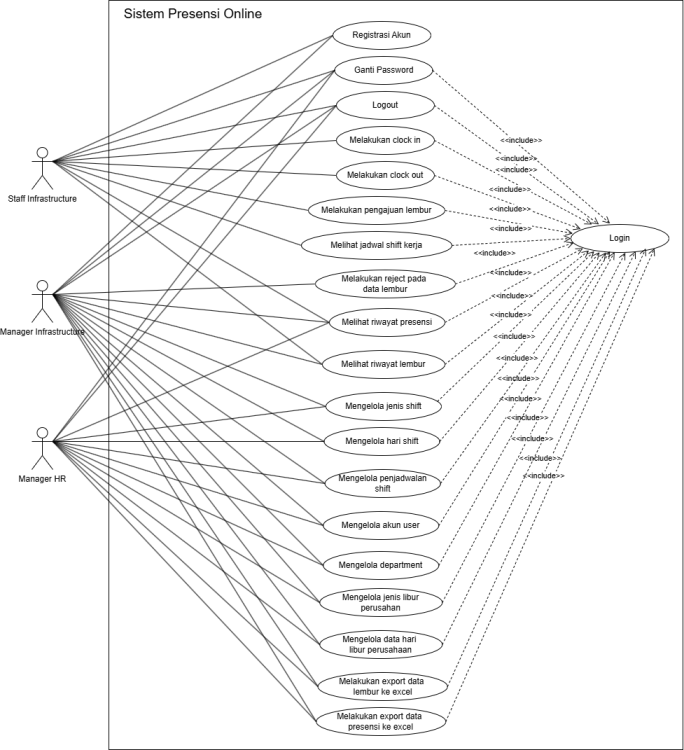
\includegraphics[width=13cm]{Gambar/bab2/use-case-presensi-online.png}
	\caption{\textit{Use Case Diagram} Aplikasi Presensi \textit{Online}}
	\label{fig:use-case-diagram-aplikasi-presensi-online}
\end{figure}
% Kembali ke penomoran bab 3 setelah gambar ini
% \renewcommand{\thefigure}{\thechapter.\arabic{figure}}
% \setcounter{figure}{0} % Optional, jika ingin mengatur ulang
\end{landscape}

\nextappendix
\section*{Lampiran \theappendixletter: \textit{Use Case Scenario} Aplikasi Presensi \textit{Online} 
\label{sec:use-case-scenario-aplikasi-presensi-online}}
\addcontentsline{toc}{section}{Lampiran \theappendixletter: \textit{Use Case Scenario} Aplikasi Presensi \textit{Online}}
\begin{longtable}{ |p{6cm}|p{8cm}|}
\caption{\textit{Use Case Scenario} Registrasi Akun}\label{tab:use-case-scenario-registrasi-akun} 
\\
\hline
\textbf{\textit{Use Case Name}}
&Registrasi Akun 
\\ \hline

\textbf{\textit{Actor}}
&\textit{Staff Infrastructure}, \textit{Manager Infrastructure} 
\\ \hline

\textbf{\textit{Brief Description}}
&\textit{Actor} yang tidak memiliki akun untuk \textit{login} dapat melakukan registrasi akun
\\ \hline

\textbf{\textit{Entry Conditions}}
&\textit{Actor} telah mengakses menu registrasi akun
\\ \hline

\textbf{\textit{Flow of event}}
&1. \textit{Actor} membuka menu registasi akun
\newline
2. \textit{Actor} mengisi seluruh \textit{form input} regitrasi akun dan menekan tombol \textit{submit}
\newline
3. Sistem menampilkan \textit{modal} verifikasi \textit{email} dan mengirimkan kode OTP ke \textit{email} \textit{actor}
\newline
4. \textit{Actor} mengisi kode OTP yang didapatkan melalui \textit{email}
\newline
5. \textit{Actor} menunggu akun diaktifkan oleh \textit{Manager}
\\ \hline

\textbf{\textit{Alternative scenario}}
&\textit{Actor} mengisi \textit{input email} pada \textit{form registrasi} dengan \textit{email} selain domain perusahaan dan sudah terdaftar maka : Sistem menampilkan pesan error
\\ \hline

\textbf{\textit{Exit Conditions}}
&Sistem menampilkan menu \textit{login}
\\ \hline
\end{longtable}

%%%%%%%%%%%%%%%%%%%%%%%%%%%%%%%%%%%%%%%%%%%%%%%%
\begin{longtable}{ |p{6cm}|p{8cm}|}
\caption{\textit{Use Case Scenario} Ganti Password}\label{tab:use-case-scenario-ganti-password} 
\\
\hline
\textbf{\textit{Use Case Name}}
&Ganti Password
\\ \hline

\textbf{\textit{Actor}}
&\textit{Staff Infrastructure}, \textit{Manager Infrastructure}, \textit{Manager Human Resources}
\\ \hline

\textbf{\textit{Brief Description}}
&\textit{Actor} yang ingin mengganti password akun
\\ \hline

\textbf{\textit{Entry Conditions}}
&\textit{Actor} telah melakukan \textit{login}
\\ \hline

\textbf{\textit{Flow of event}}
&1. \textit{Actor} membuka menu profil dan menekan tombol \textit{change password}
\newline
2. \textit{Actor} mengisi seluruh \textit{form input} pergantian password dan menekan tombol \textit{submit}
\newline
\\ \hline

\textbf{\textit{Alternative scenario}}
&\textit{Actor} yang salah mengisi password lama maka sistem akan mengembalikan pesan kesalahan
\\ \hline

\textbf{\textit{Exit Conditions}}
&Sistem selesai memproses pergantian passowrd dan menampilkan pesan berhasil ganti password
\\ \hline
\end{longtable}

%%%%%%%%%%%%%%%%%%%%%%%%%%%%%%%%%%%%%%%%%%%%%%%%%%%%%%%%%%%%%%%%%
\FloatBarrier
\begin{longtable}{ |p{6cm}|p{8cm}|}
\caption{\textit{Use Case Scenario Login}}\label{tab:use-case-scenario-login} 
\\
\hline
\textbf{\textit{Use Case Name}}
&\textit{Login}
\\ \hline

\textbf{\textit{Actor}}
&\textit{Staff Infrastructure}, \textit{Manager Infrastructure}, \textit{Manager Human Resources} 
\\ \hline

\textbf{\textit{Brief Description}}
&\textit{Actor} yang ingin masuk ke dalam menu utama dan menggunakan seluruh fitur didalam aplikasi
\\ \hline

\textbf{\textit{Entry Conditions}}
&\textit{Actor} yang telah melakukan regitrasi akun dan akun sudah berstatus aktif
\\ \hline

\textbf{\textit{Flow of event}}
&1. \textit{Actor} membuka halaman \textit{login}
\newline
2. \textit{Actor} mengisi seluruh \textit{form input} login dan menekan tombol \textit{login}
\newline
3. Sistem melakukan pengecekkan terhadap \textit{credential} dari \textit{user}
\newline
4. Sistem regenerasi \textit{session} pada \textit{user}
\\ \hline

\textbf{\textit{Alternative scenario}}
&1. \textit{Actor} yang salah mengisi \textit{form input email} atau \textit{password} maka: Sistem menampilkan pesan error
\newline
2. \textit{Actor} yang sudah \textit{login} sebelumnya dan sistem akan mengecek \textit{session} dari \textit{user}, kemudian mengarahkan \textit{user} ke halaman utama
\\ \hline

\textbf{\textit{Exit Conditions}}
&Sistem menampilkan menu utama dengan fitur yang sesuai masing-masing \textit{position} dan \textit{department}
\\ \hline
\end{longtable}

%%%%%%%%%%%%%%%%%%%%%%%%%%%%%%%%%%%%%%%%%%%%%%%%%%%%%%%%%%%%%%%%%
\FloatBarrier
\begin{longtable}{ |p{6cm}|p{8cm}|}
\caption{\textit{Use Case Scenario Logout}}\label{tab:use-case-scenario-logout} 
\\
\hline
\textbf{\textit{Use Case Name}}
&\textit{Logout}
\\ \hline

\textbf{\textit{Actor}}
&\textit{Staff Infrastructure}, \textit{Manager Infrastructure}, \textit{Manager Human Resources} 
\\ \hline

\textbf{\textit{Brief Description}}
&\textit{Actor} yang telah melakukan \textit{login} dan ingin keluar dari sesi \textit{login}
\\ \hline

\textbf{\textit{Entry Conditions}}
&\textit{Actor} yang sudah melakukan \textit{login}
\\ \hline

\textbf{\textit{Flow of event}}
&1. \textit{Actor} menekan tombol yang bergambar \textit{profile user} pada \textit{navbar}
\newline
2. Sistem akan menampilkan beberapa pilihan, \textit{actor} menekan pilihan \textit{logout}
\newline
3. Sistem akan melakukan \textit{logout} dan menghapus \textit{session} dari \textit{user}
\\ \hline

\textbf{\textit{Alternative scenario}}
&-
\\ \hline

\textbf{\textit{Exit Conditions}}
&Sistem menampilkan menu \textit{login}
\\ \hline
\end{longtable}

%%%%%%%%%%%%%%%%%%%%%%%%%%%%%%%%%%%%%%%%%%%%%%%%%%%%%%%%%%%%%%%%%
\FloatBarrier
\begin{longtable}{ |p{6cm}|p{8cm}|}
\caption{\textit{Use Case Scenario Melakukan Clock In}}\label{tab:use-case-scenario-clock-in} 
\\
\hline
\textbf{\textit{Use Case Name}}
&\textit{Melakukan clock In}
\\ \hline

\textbf{\textit{Actor}}
&\textit{Staff Infrastructure}
\\ \hline

\textbf{\textit{Brief Description}}
&\textit{Actor} yang melakukan presensi masuk
\\ \hline

\textbf{\textit{Entry Conditions}}
&\textit{Actor} yang sudah melakukan \textit{login} dan belum melakukan \textit{clock in} sebelumnya
\\ \hline

\textbf{\textit{Flow of event}}
&1. \textit{Actor} menekan tombol \textit{presence} pada navbar
\newline
2. Sistem akan tampilan halaman \textit{presence}
\newline
3. \textit{Actor} menekan tombol \textit{clock in}
\newline
4. Sistem akan menampikan \textit{pop up modal} yang berisi tombol untuk pengambilan lokasi dan foto
\newline
5. \textit{Actor} menekan tombol \textit{get my location} untuk meng-\textit{input} lokasi \textit{user} secara otomatis melalui GPS dan \textit{Actor} menekan tombol \textit{take photo} untuk membuka kamera dan melakukan pengambilan foto
\newline
6. Mengisi \textit{form input} informasi presensi , kemudian menekan tombol \textit{clock in now}
\newline
7. Sistem akan menyimpan data presensi \textit{actor}
\\ \hline

\textbf{\textit{Alternative scenario}}
&\textit{Actor} yang sudah melakukan \textit{clock in} saat terakhir kali maka : tombol \textit{clock in} akan ter-\textit{disabled}
\\ \hline

\textbf{\textit{Exit Conditions}}
&Sistem selesai memproses data presensi masuk dan menampilkan \textit{pop up message} berhasil \textit{clock in}
\\ \hline
\end{longtable}


%%%%%%%%%%%%%%%%%%%%%%%%%%%%%%%%%%%%%%%%%%%%%%%%%%%%%%%%%%%%%%%%%
\FloatBarrier
\begin{longtable}{ |p{6cm}|p{8cm}|}
\caption{\textit{Use Case Scenario} Melakukan \textit{Clock Out}}\label{tab:use-case-scenario-clock-out} 
\\
\hline
\textbf{\textit{Use Case Name}}
&Melakukan \textit{clock Out}
\\ \hline

\textbf{\textit{Actor}}
&\textit{Staff Infrastructure}
\\ \hline

\textbf{\textit{Brief Description}}
&\textit{Actor} yang melakukan presensi keluar
\\ \hline

\textbf{\textit{Entry Conditions}}
&\textit{Actor} yang sudah melakukan \textit{login} dan sudah melakukan \textit{clock in} sebelumnya
\\ \hline

\textbf{\textit{Flow of event}}
&1. \textit{Actor} menekan tombol \textit{presence} pada navbar
\newline
2. Sistem akan tampilan halaman \textit{presence}
\newline
3. \textit{Actor} menekan tombol \textit{clock out}
\newline
4. Sistem akan menampikan \textit{pop up modal} yang berisi tombol untuk pengambilan lokasi dan foto
\newline
5. \textit{Actor} menekan tombol \textit{get my location} untuk meng-\textit{input} lokasi \textit{user} secara otomatis melalui GPS dan \textit{Actor} menekan tombol \textit{take photo} untuk membuka kamera dan melakukan pengambilan foto
\newline
6. Mengisi \textit{input form} informasi presensi, kemudian menekan tombol \textit{clock out now}
\newline
7. Sistem akan menyimpan data presensi \textit{actor}, dan sistem akan mengecek pada data presensi saat \textit{clock in} dan \textit{clock out} dan menyimpan data lembur jika presensi dilakukan diluar jam \textit{shift} kerja atau hari libur
\newline
8. Jika terdapat data lembur, sistem menyimpan data lembur
\\ \hline

\textbf{\textit{Alternative scenario}}
&\textit{Actor} yang belum melakukan \textit{clock in} saat terakhir kali maka : tombol \textit{clock out} akan ter-\textit{disabled}
\\ \hline

\textbf{\textit{Exit Conditions}}
&Sistem selesai memproses data presensi keluar dan data lembur, kemudian menampilkan \textit{pop up message} berhasil \textit{clock out}
\\ \hline
\end{longtable}


%%%%%%%%%%%%%%%%%%%%%%%%%%%%%%%%%%%%%%%%%%%%%%%%%%%%%%%%%%%%%%%%%
\FloatBarrier
\begin{longtable}{ |p{6cm}|p{8cm}|}
\caption{\textit{Use Case Scenario} Melakukan Pengajuan Lembur}\label{tab:use-case-scenario-melakukan-pengajuan-lembur} 
\\
\hline
\textbf{\textit{Use Case Name}}
&Melakukan pengajuan lembur
\\ \hline

\textbf{\textit{Actor}}
&\textit{Staff Infrastructure}
\\ \hline

\textbf{\textit{Brief Description}}
&\textit{Actor} yang melakukan pengajuan lembur
\\ \hline

\textbf{\textit{Entry Conditions}}
&\textit{Actor} yang sudah melakukan \textit{login} dan ingin mengajukan lembur karena lupa presensi saat jam lembur
\\ \hline

\textbf{\textit{Flow of event}}
&1. \textit{Actor} menekan tombol \textit{request} pada navbar
\newline
2. Sistem akan menampilkan halaman \textit{overtime correction request}
\newline
3. \textit{Actor} mengisi seluruh \textit{form input} pada halaman \textit{overtime correction request} dan menekan tombol submit
\newline
4. Sistem akan menyimpan data lembur yang telah diisi oleh \textit{actor}
\\ \hline

\textbf{\textit{Alternative scenario}}
&\textit{Actor} yang tidak mengisi seluruh \textit{input form} maka : Sistem akan memberikan pesan error
\\ \hline

\textbf{\textit{Exit Conditions}}
&Sistem selesai memproses data lembur dan menampilkan \textit{pop up message} berhasil dan mengembalikan tampilan ke halaman \textit{overtime correction request}
\\ \hline
\end{longtable}

%%%%%%%%%%%%%%%%%%%%%%%%%%%%%%%%%%%%%%%%%%%%%%%%%%%%%%%%%%%%%%%%%
\FloatBarrier
\begin{longtable}{ |p{6cm}|p{8cm}|}
\caption{\textit{Use Case Scenario} Melihat Jadwal \textit{Shift} Kerja}\label{tab:use-case-scenario-melihat-jadwal-shift-kerja} 
\\
\hline
\textbf{\textit{Use Case Name}}
&Melihat jadwal \textit{shift} kerja
\\ \hline

\textbf{\textit{Actor}}
&\textit{Staff Infrastructure}
\\ \hline

\textbf{\textit{Brief Description}}
&\textit{Actor} yang melihat jadwal \textit{shift} kerja
\\ \hline

\textbf{\textit{Entry Conditions}}
&\textit{Actor} yang sudah melakukan \textit{login} dan ingin melihat jadwal \textit{shift} kerja
\\ \hline

\textbf{\textit{Flow of event}}
&1. \textit{Actor} menekan tombol \textit{presence} pada \textit{navbar}
\newline
2. Sistem akan menampilkan halaman \textit{presence}
\newline
3. \textit{Actor} menekan tombol \textit{shift schedule}
\newline
4. Sistem akan menampilkan jadwal kerja \textit{actor}
\\ \hline

\textbf{\textit{Alternative scenario}}
&\textit{Actor} yang tidak memiliki jadwal kerja maka tidak akan ada data yang ditampilkan
\\ \hline

\textbf{\textit{Exit Conditions}}
&\textit{Actor} menutup \textit{modal} data \textit{shift} dan sistem menampilkan kembali halaman \textit{attendance}
\\ \hline
\end{longtable}

%%%%%%%%%%%%%%%%%%%%%%%%%%%%%%%%%%%%%%%%%%%%%%%%%%%%%%%%%%%%%%%%%
\FloatBarrier
\begin{longtable}{ |p{6cm}|p{8cm}|}
\caption{\textit{Use Case Scenario} Melakukan \textit{Reject} Pada Data Lembur}\label{tab:use-case-scenario-melakukan-approval} 
\\
\hline
\textbf{\textit{Use Case Name}}
&Melakukan \textit{reject} pada data lembur
\\ \hline

\textbf{\textit{Actor}}
&\textit{Manager Infrastructure}
\\ \hline

\textbf{\textit{Brief Description}}
&\textit{Actor} yang melakukan \textit{reject} pada data lembur
\\ \hline

\textbf{\textit{Entry Conditions}}
&\textit{Actor} yang sudah melakukan \textit{login} dan ingin melakukan penolakkan atau \textit{reject} pada data lembur yang masuk
\\ \hline

\textbf{\textit{Flow of event}}
&1. \textit{Actor} menekan tombol \textit{reject} pada \textit{navbar}
\newline
2. Sistem akan menampilkan \textit{list} data \textit{lembur} yang tidak pernah di-\textit{reject}
\newline
3. \textit{Actor} melakukan \textit{reject} pada data yang dipilih atau mencetang \textit{checkbox} pada data lembur dan menekan tombol \textit{reject selected}
\newline
5. \textit{Actor} melakukan konfirmasi perubahan
\newline
6. Sistem menyimpan perubahan data
\\ \hline

\textbf{\textit{Alternative scenario}}
&-
\\ \hline

\textbf{\textit{Exit Conditions}}
&Sistem selesai memproses seluruh perubahan data lembur dan kembali menampilkan halaman \textit{reject}
\\ \hline
\end{longtable}

%%%%%%%%%%%%%%%%%%%%%%%%%%%%%%%%%%%%%%%%%%%%%%%%%%%%%%%%%%%%%%%%%
\FloatBarrier
\begin{longtable}{ |p{6cm}|p{8cm}|}
\caption{\textit{Use Case Scenario} Melakukan \textit{Export} Data Lembur ke \textit{Excel}}\label{tab:use-case-scenario-melakukan-export-data-lembur} 
\\
\hline
\textbf{\textit{Use Case Name}}
&Melakukan \textit{Export} Data Lembur ke \textit{Excel}
\\ \hline

\textbf{\textit{Actor}}
&\textit{Manager Human Resources, Manager Infrastructure}
\\ \hline

\textbf{\textit{Brief Description}}
&\textit{Actor} yang melakukan \textit{export} data lembur menjadi format \textit{Excel}
\\ \hline

\textbf{\textit{Entry Conditions}}
&\textit{Actor} yang sudah melakukan \textit{login} dan ingin melakukan \textit{export} data lembur menjadi format \textit{Excel}
\\ \hline

\textbf{\textit{Flow of event}}
&1. \textit{Actor} menekan tombol \textit{overtime history} pada \textit{navbar}
\newline
2. Sistem akan menampilkan \textit{list} data riwayat lembur
\newline
3. \textit{Actor} melakukan \textit{filter} nama \textit{staff}, tanggal atau status
\newline
4. Sistem menampilkan data lembur yang telah di-\textit{filter}
\newline
5. \textit{Actor} menekan tombol \textit{Export}
\newline
6. Sistem akan memproses data lembur dan memberikan konfirmasi untuk men-\textit{download} \textit{file} dalam bentu \textit{Excel}
\newline
7. \textit{Actor} mengunduh \textit{file Excel}
\newline
\\ \hline

\textbf{\textit{Alternative scenario}}
&Jika tidak ada data lembur atau data yang di-\textit{filter} tidak ditemukan, maka sistem tidak akan memproses permintaan \textit{export}
\\ \hline

\textbf{\textit{Exit Conditions}}
&\textit{Actor} menekan konfirmasi saat pengunduhan \textit{file} dan sistem akan mengembalikan tampilan ke \textit{overtime history}
\\ \hline
\end{longtable}

%%%%%%%%%%%%%%%%%%%%%%%%%%%%%%%%%%%%%%%%%%%%%%%%%%%%%%%%%%%%%%%%%
\FloatBarrier
\begin{longtable}{ |p{6cm}|p{8cm}|}
\caption{\textit{Use Case Scenario} Melakukan \textit{Export} Data Presensi ke \textit{Excel}}\label{tab:use-case-scenario-melakukan-export-data-presensi} 
\\
\hline
\textbf{\textit{Use Case Name}}
&Melakukan \textit{Export} Data Presensi ke \textit{Excel}
\\ \hline

\textbf{\textit{Actor}}
&\textit{Manager Human Resources, Manager Infrastructure}
\\ \hline

\textbf{\textit{Brief Description}}
&\textit{Actor} yang melakukan \textit{export} data presensi menjadi format \textit{Excel}
\\ \hline

\textbf{\textit{Entry Conditions}}
&\textit{Actor} yang sudah melakukan \textit{login} dan ingin melakukan \textit{export} data presensi menjadi format \textit{Excel}
\\ \hline

\textbf{\textit{Flow of event}}
&1. \textit{Actor} menekan tombol \textit{attendance history} pada \textit{navbar}
\newline
2. Sistem akan menampilkan \textit{list} data riwayat presensi
\newline
3. \textit{Actor} melakukan \textit{filter} nama \textit{staff}, tanggal atau status
\newline
4. Sistem menampilkan data presensi yang telah di-\textit{filter}
\newline
5. \textit{Actor} menekan tombol \textit{Export}
\newline
6. Sistem akan memproses data presensi dan memberikan konfirmasi untuk men-\textit{download} \textit{file} dalam bentu \textit{Excel}
\newline
7. \textit{Actor} mengunduh \textit{file Excel}
\newline
\\ \hline

\textbf{\textit{Alternative scenario}}
&Jika tidak ada data presensi atau data yang di-\textit{filter} tidak ditemukan, maka sistem tidak akan memproses permintaan \textit{export}
\\ \hline

\textbf{\textit{Exit Conditions}}
&\textit{Actor} menekan konfirmasi saat pengunduhan \textit{file} dan sistem akan mengembalikan tampilan ke \textit{attendance history}
\\ \hline
\end{longtable}

%%%%%%%%%%%%%%%%%%%%%%%%%%%%%%%%%%%%%%%%%%%%%%%%%%%%%%%%%%%%%%%%%
\FloatBarrier
\begin{longtable}{ |p{6cm}|p{8cm}|}
\caption{\textit{Use Case Scenario} Melihat Riwayat Lembur}\label{tab:use-case-scenario-melihat-riwayat-lembur} 
\\
\hline
\textbf{\textit{Use Case Name}}
&Melihat riwayat lembur
\\ \hline

\textbf{\textit{Actor}}
&\textit{Staff Infrastructure}, \textit{Manager Infrastructure}, \textit{Manager Human Resources}
\\ \hline

\textbf{\textit{Brief Description}}
&\textit{Actor} yang melihat riwayat lembur
\\ \hline

\textbf{\textit{Entry Conditions}}
&\textit{Actor} yang sudah melakukan \textit{login} dan ingin melihat riwayat lembur
\\ \hline

\textbf{\textit{Flow of event}}
&1. \textit{Actor} menekan tombol \textit{overtime history} pada \textit{navbar}
\newline
2. Sistem akan menampilkan \textit{list} data riwayat lembur
\newline
3. \textit{Actor} melakukan \textit{filter} tanggal dan status pada data lembur untuk mencari spesifik data lembur
\newline
4. \textit{Actor} menekan tombol \textit{details} pada salah satu data lembur
\newline
5. Sistem menampilkan halaman \textit{details} dan informasi lengkap terkait data lembur yang dipilih
\newline
\\ \hline

\textbf{\textit{Alternative scenario}}
&Jika tidak ada data lembur atau data yang di-\textit{filter} tidak ditemukan, maka sistem tidak akan menampilkan data
\\ \hline

\textbf{\textit{Exit Conditions}}
&\textit{Actor} menekan tombol kembali dan sistem akan menampilkan kembali halaman \textit{overtime history}
\\ \hline
\end{longtable}

%%%%%%%%%%%%%%%%%%%%%%%%%%%%%%%%%%%%%%%%%%%%%%%%%%%%%%%%%%%%%%%%%
\FloatBarrier
\begin{longtable}{ |p{6cm}|p{8cm}|}
\caption{\textit{Use Case Scenario} Melihat Riwayat Presensi}\label{tab:use-case-scenario-melihat-riwayat-presensi} 
\\
\hline
\textbf{\textit{Use Case Name}}
&Melihat riwayat presensi
\\ \hline

\textbf{\textit{Actor}}
&\textit{Staff Infrastructure}, \textit{Manager Infrastructure}, \textit{Manager Human Resources}
\\ \hline

\textbf{\textit{Brief Description}}
&\textit{Actor} yang melihat riwayat presensi
\\ \hline

\textbf{\textit{Entry Conditions}}
&\textit{Actor} yang sudah melakukan \textit{login} dan ingin melihat riwayat presensi
\\ \hline

\textbf{\textit{Flow of event}}
&1. \textit{Actor} menekan tombol \textit{attendance history} pada \textit{navbar}
\newline
2. Sistem akan menampilkan \textit{list} data riwayat presensi
\newline
3. \textit{Actor} melakukan \textit{filter} tanggal pada data presensi untuk mencari spesifik data presensi
\newline
4. \textit{Actor} menekan tombol \textit{details} pada salah satu data presensi
\newline
5. Sistem menampilkan halaman \textit{details} dan informasi lengkap terkait data presensi yang dipilih
\newline
\\ \hline

\textbf{\textit{Alternative scenario}}
&Jika tidak ada data presensi atau data yang di-\textit{filter} tidak ditemukan, maka sistem tidak akan menampilkan data
\\ \hline

\textbf{\textit{Exit Conditions}}
&\textit{Actor} menekan tombol kembali dan sistem akan menampilkan kembali halaman \textit{attendance history}
\\ \hline
\end{longtable}

%%%%%%%%%%%%%%%%%%%%%%%%%%%%%%%%%%%%%%%%%%%%%%%%%%%%%%%%%%%%%%%%%
\FloatBarrier
\begin{longtable}{ |p{6cm}|p{8cm}|}
\caption{\textit{Use Case Scenario} Mengelola Jenis \textit{Shift}}\label{tab:use-case-scenario-mengelola-jenis-shift} 
\\
\hline
\textbf{\textit{Use Case Name}}
&Mengelola jenis \textit{shift}
\\ \hline

\textbf{\textit{Actor}}
&\textit{Manager Human Resources}, \textit{Manager Infrastructure}
\\ \hline

\textbf{\textit{Brief Description}}
&\textit{Actor} yang mengelola jenis \textit{shift}
\\ \hline

\textbf{\textit{Entry Conditions}}
&\textit{Actor} yang sudah melakukan \textit{login} dan ingin mengelola jenis \textit{shift}
\\ \hline

\textbf{\textit{Flow of event}}
&1. \textit{Actor} menekan tombol \textit{shift} pada \textit{navbar}
\newline
2. Sistem akan menampilkan halaman \textit{shift} beserta data jenis \textit{shift} kerja
\newline
3. \textit{Actor} mengelola (\textit{create, update, delete}) data jenis \textit{shift}
    \newline
4. Sistem menampilkan konfirmasi perubahan data
\newline
5. \textit{Actor} melakukan konfirmasi perubahan
\newline
6. Sistem menyimpan perubahan data
\newline
\\ \hline

\textbf{\textit{Alternative scenario}}
&\textit{Actor} yang tidak melakukan konfirmasi perubahan data maka sistem tidak akan menyimpan perubahan data
\\ \hline

\textbf{\textit{Exit Conditions}}
&Sistem selesai memproses seluruh perubahan data jenis \textit{shift} dan kembali menampilkan halaman \textit{shift}
\\ \hline
\end{longtable}

%%%%%%%%%%%%%%%%%%%%%%%%%%%%%%%%%%%%%%%%%%%%%%%%%%%%%%%%%%%%%%%%%
\FloatBarrier
\begin{longtable}{ |p{6cm}|p{8cm}|}
\caption{\textit{Use Case Scenario} Mengelola Hari \textit{Shift}}\label{tab:use-case-scenario-mengelola-hari-shift} 
\\
\hline
\textbf{\textit{Use Case Name}}
&Mengelola hari \textit{shift}
\\ \hline

\textbf{\textit{Actor}}
&\textit{Manager Human Resources}, \textit{Manager Infrastructure}
\\ \hline

\textbf{\textit{Brief Description}}
&\textit{Actor} yang mengelola hari \textit{shift}
\\ \hline

\textbf{\textit{Entry Conditions}}
&\textit{Actor} yang sudah melakukan \textit{login} dan ingin mengelola hari \textit{shift}
\\ \hline

\textbf{\textit{Flow of event}}
&1. \textit{Actor} menekan \textit{edit} pada salah satu jenis \textit{shift} melalui halaman \textit{shift}
\newline
2. Sistem akan menampilkan \textit{modal} hari \textit{shift} beserta data hari \textit{shift} kerja
\newline
3. \textit{Actor} mengelola (\textit{create, update, delete}) data hari \textit{shift}
    \newline
4. Sistem menampilkan konfirmasi perubahan data
\newline
5. \textit{Actor} melakukan konfirmasi perubahan
\newline
6. Sistem menyimpan perubahan data
\newline
\\ \hline

\textbf{\textit{Alternative scenario}}
&\textit{Actor} yang tidak melakukan konfirmasi perubahan data maka sistem tidak akan menyimpan perubahan data
\\ \hline

\textbf{\textit{Exit Conditions}}
&Sistem selesai memproses seluruh perubahan data hari \textit{shift} dan kembali menampilkan halaman \textit{shift}
\\ \hline
\end{longtable}

%%%%%%%%%%%%%%%%%%%%%%%%%%%%%%%%%%%%%%%%%%%%%%%%%%%%%%%%%%%%%%%%%
\FloatBarrier
\begin{longtable}{ |p{6cm}|p{8cm}|}
\caption{\textit{Use Case Scenario} Mengelola Penjadwalan \textit{Shift}}\label{tab:use-case-scenario-mengelola-penjadwalan-shift}
\\
\hline
\textbf{\textit{Use Case Name}}
&Mengelola penjadwalan \textit{shift}
\\ \hline

\textbf{\textit{Actor}}
&\textit{Manager Human Resources}, \textit{Manager Infrastructure}
\\ \hline

\textbf{\textit{Brief Description}}
&\textit{Actor} yang mengelola penjadwalan \textit{shift}
\\ \hline

\textbf{\textit{Entry Conditions}}
&\textit{Actor} yang sudah melakukan \textit{login} dan ingin mengelola penjadwalan \textit{shift}
\\ \hline

\textbf{\textit{Flow of event}}
&1. \textit{Actor} menekan tombol \textit{shift scheduling} pada \textit{navbar}
\newline
2. Sistem akan menampilkan halaman penjadwalan \textit{shift} beserta data penjadwalan \textit{shift} kerja
\newline
3. \textit{Actor} mengelola (\textit{create, update, delete, import}) data penjadwalan \textit{shift}
    \newline
4. Sistem menampilkan konfirmasi perubahan data
\newline
5. \textit{Actor} melakukan konfirmasi perubahan
\newline
6. Sistem menyimpan perubahan data
\newline
\\ \hline

\textbf{\textit{Alternative scenario}}
&\textit{Actor} yang tidak melakukan konfirmasi perubahan data maka sistem tidak akan menyimpan perubahan data
\\ \hline

\textbf{\textit{Exit Conditions}}
&Sistem selesai memproses seluruh perubahan data penjadwalan \textit{shift} dan kembali menampilkan halaman penjadwalan \textit{shift}
\\ \hline
\end{longtable}


%%%%%%%%%%%%%%%%%%%%%%%%%%%%%%%%%%%%%%%%%%%%%%%%%%%%%%%%%%%%%%%%%
\FloatBarrier
\begin{longtable}{ |p{6cm}|p{8cm}|}
\caption{\textit{Use Case Scenario} Mengelola Akun \textit{User}}\label{tab:use-case-scenario-mengelola-akun-user} 
\\
\hline
\textbf{\textit{Use Case Name}}
&Mengelola akun \textit{user}
\\ \hline

\textbf{\textit{Actor}}
&\textit{Manager Human Resources}, \textit{Manager Infrastructure}
\\ \hline

\textbf{\textit{Brief Description}}
&\textit{Actor} yang mengelola akun \textit{user}
\\ \hline

\textbf{\textit{Entry Conditions}}
&\textit{Actor} yang sudah melakukan \textit{login} dan ingin mengelola akun \textit{user}
\\ \hline

\textbf{\textit{Flow of event}}
&1. \textit{Actor} menekan tombol \textit{user} pada \textit{navbar}
\newline
2. Sistem akan menampilkan halaman \textit{user} beserta data semua \textit{user}
\newline
3. \textit{Actor} mengelola \textit{update, delete} data akun \textit{user}
\newline
4. Sistem menampilkan konfirmasi perubahan data
\newline
5. \textit{Actor} melakukan konfirmasi perubahan
\newline
6. Sistem menyimpan perubahan data
\\ \hline

\textbf{\textit{Alternative scenario}}
&\textit{Actor} yang tidak melakukan konfirmasi perubahan data maka sistem tidak akan menyimpan perubahan data
\\ \hline

\textbf{\textit{Exit Conditions}}
&Sistem selesai memproses seluruh perubahan data \textit{user} dan kembali menampilkan halaman \textit{user}
\\ \hline
\end{longtable}

%%%%%%%%%%%%%%%%%%%%%%%%%%%%%%%%%%%%%%%%%%%%%%%%%%%%%%%%%%%%%%%%%
\FloatBarrier
\begin{longtable}{ |p{6cm}|p{8cm}|}
\caption{\textit{Use Case Scenario} Mengelola \textit{Department}}\label{tab:use-case-scenario-mengelola-department} 
\\
\hline
\textbf{\textit{Use Case Name}}
&Mengelola \textit{department}
\\ \hline

\textbf{\textit{Actor}}
&\textit{Manager Human Resources}, \textit{Manager Infrastructure}
\\ \hline

\textbf{\textit{Brief Description}}
&\textit{Actor} yang mengelola \textit{department}
\\ \hline

\textbf{\textit{Entry Conditions}}
&\textit{Actor} yang sudah melakukan \textit{login} dan ingin mengelola \textit{department}
\\ \hline

\textbf{\textit{Flow of event}}
&1. \textit{Actor} menekan tombol \textit{department} pada \textit{navbar}
\newline
2. Sistem akan menampilkan halaman \textit{department} beserta data semua \textit{department}
\newline
3. \textit{Actor} mengelola \textit{update, delete} data akun \textit{department}
\newline
4. Sistem menampilkan konfirmasi perubahan data
\newline
5. \textit{Actor} melakukan konfirmasi perubahan
\newline
6. Sistem menyimpan perubahan data
\\ \hline

\textbf{\textit{Alternative scenario}}
&\textit{Actor} yang tidak melakukan konfirmasi perubahan data maka sistem tidak akan menyimpan perubahan data
\\ \hline

\textbf{\textit{Exit Conditions}}
&Sistem selesai memproses seluruh perubahan data \textit{department} dan kembali menampilkan halaman \textit{department}
\\ \hline
\end{longtable}

%%%%%%%%%%%%%%%%%%%%%%%%%%%%%%%%%%%%%%%%%%%%%%%%%%%%%%%%%%%%%%%%%
\FloatBarrier
\begin{longtable}{ |p{6cm}|p{8cm}|}
\caption{\textit{Use Case Scenario} Mengelola Jenis Libur Perusahaan}\label{tab:use-case-scenario-mengelola-jenis-libur-perusahaan} 
\\
\hline
\textbf{\textit{Use Case Name}}
&Mengelola jenis libur perusahaan
\\ \hline

\textbf{\textit{Actor}}
&\textit{Manager Human Resources}, \textit{Manager Infrastructure}
\\ \hline

\textbf{\textit{Brief Description}}
&\textit{Actor} yang mengelola jenis libur perusahaan
\\ \hline

\textbf{\textit{Entry Conditions}}
&\textit{Actor} yang sudah melakukan \textit{login} dan ingin mengelola jenis libur perusahaan
\\ \hline

\textbf{\textit{Flow of event}}
&1. \textit{Actor} menekan tombol libur pada \textit{navbar}
\newline
2. Sistem akan menampilkan halaman libur beserta seluruh data jenis libur perusahaan
\newline
3. \textit{Actor} mengelola (\textit{create, update, delete}) data jenis libur perusahaan
\newline
4. Sistem menampilkan konfirmasi perubahan data
\newline
5. \textit{Actor} melakukan konfirmasi perubahan
\newline
6. Sistem menyimpan perubahan data
\\ \hline

\textbf{\textit{Alternative scenario}}
&1. \textit{Actor} yang tidak melakukan konfirmasi perubahan data maka sistem tidak akan menyimpan perubahan data
\newline
2. Jika tidak ada data hari libur yang ditemukan, maka sistem tidak akan menampilkan hasil
\\ \hline

\textbf{\textit{Exit Conditions}}
&Sistem selesai memproses seluruh perubahan data jenis libur perusahaan dan kembali menampilkan halaman jenis libur
\\ \hline
\end{longtable}

%%%%%%%%%%%%%%%%%%%%%%%%%%%%%%%%%%%%%%%%%%%%%%%%%%%%%%%%%%%%%%%%%
\FloatBarrier
\begin{longtable}{ |p{6cm}|p{8cm}|}
\caption{\textit{Use Case Scenario} Mengelola Data Hari Libur Perusahaan}\label{tab:use-case-scenario-mengelola-data-hari-libur-perusahaan} 
\\
\hline
\textbf{\textit{Use Case Name}}
&Mengelola data hari libur perusahaan
\\ \hline

\textbf{\textit{Actor}}
&\textit{Manager Human Resources}, \textit{Manager Infrastructure}
\\ \hline

\textbf{\textit{Brief Description}}
&\textit{Actor} yang mengelola data hari libur perusahaan
\\ \hline

\textbf{\textit{Entry Conditions}}
&\textit{Actor} yang sudah melakukan \textit{login} dan ingin mengelola data hari libur perusahaan
\\ \hline

\textbf{\textit{Flow of event}}
&1. \textit{Actor} menekan tombol edit pada jenis libur perusahaan
\newline
2. Sistem akan menampilkan halaman hari libur beserta seluruh data hari libur perusahaan
\newline
3. \textit{Actor} mengelola (\textit{create, update, delete}) data hari libur perusahaan atau \textit{import} data hari libur nasional melalui tombol yang terhubung dengan API
\newline
4. Sistem menampilkan konfirmasi perubahan data
\newline
5. \textit{Actor} melakukan konfirmasi perubahan
\newline
6. Sistem menyimpan perubahan data
\\ \hline

\textbf{\textit{Alternative scenario}}
&1. \textit{Actor} yang tidak melakukan konfirmasi perubahan data maka sistem tidak akan menyimpan perubahan data
\newline
2. Jika tidak ada data hari libur yang ditemukan, maka sistem tidak akan menampilkan hasil
\\ \hline

\textbf{\textit{Exit Conditions}}
&Sistem selesai memproses seluruh perubahan data hari libur perusahaan dan kembali menampilkan halaman hari libur
\\ \hline
\end{longtable}


\pagebreak

\nextappendix
\section*{Lampiran \theappendixletter: \textit{Activity Diagram} Aplikasi Presensi \textit{Online} 
\label{sec:activity-diagram-aplikasi-presensi-online}}
\addcontentsline{toc}{section}{Lampiran \theappendixletter: \textit{Activity Diagram} Aplikasi Presensi \textit{Online}}
\begin{figure}[H]
	\centering
	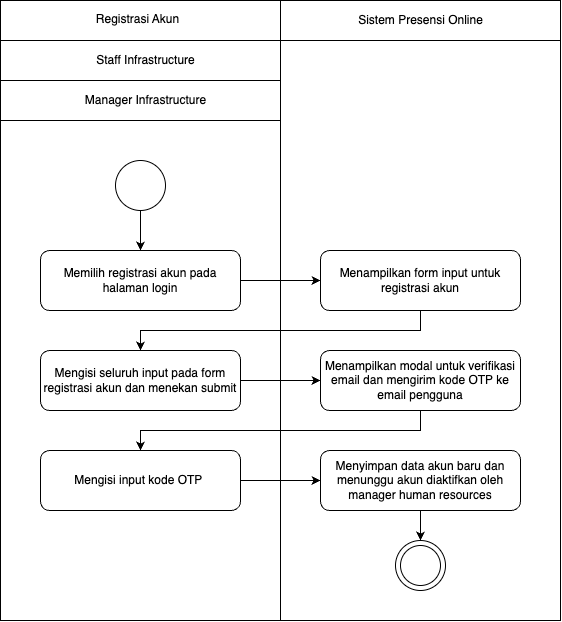
\includegraphics[width=15cm]{Gambar/bab2/activity-diagram-registrasi.png}
	\caption{\textit{Activity Diagram} Registrasi Akun}
	\label{fig:activity-diagram-registrasi}
\end{figure}
\FloatBarrier

\begin{figure}[H]
	\centering
	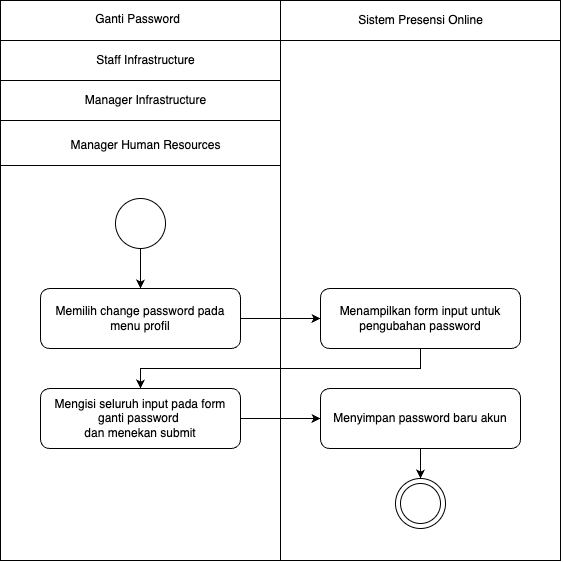
\includegraphics[width=15cm]{Gambar/bab2/activity-diagram-ganti-password.png}
	\caption{\textit{Activity Diagram} Ganti Password}
	\label{fig:activity-diagram-ganti-password}
\end{figure}
\FloatBarrier

\begin{figure}[H]
	\centering
	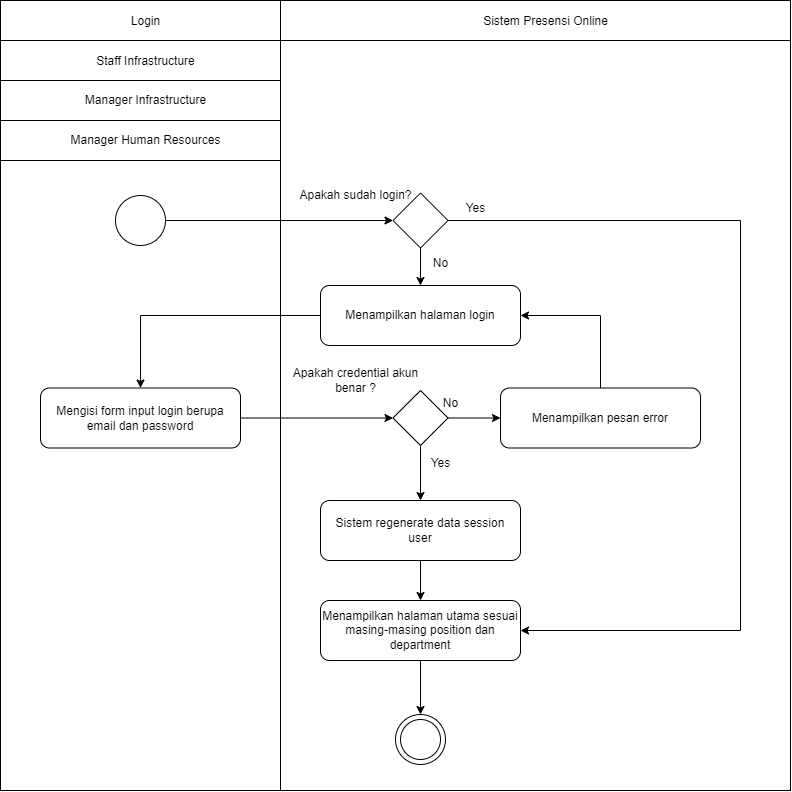
\includegraphics[width=15cm]{Gambar/bab2/activity-diagram-login.png}
	\caption{\textit{Activity Diagram Login}}
	\label{fig:activity-diagram-login}
\end{figure}
\FloatBarrier

\begin{figure}[H]
	\centering
	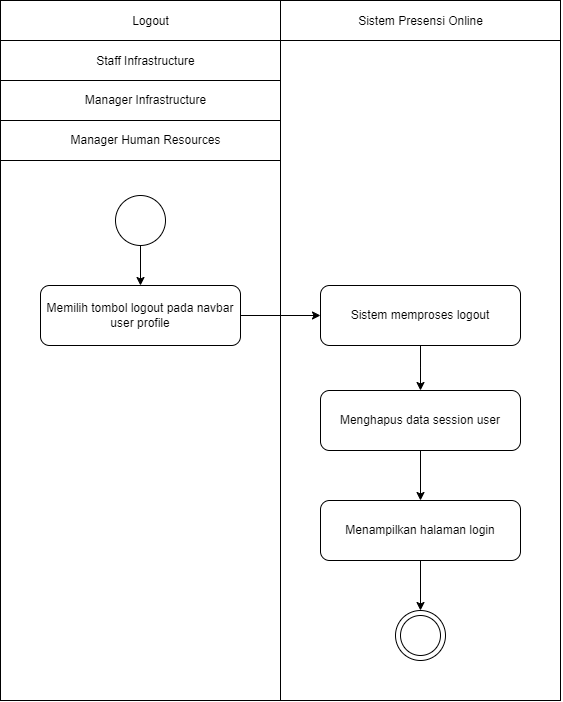
\includegraphics[width=15cm]{Gambar/bab2/activity-diagram-logout.png}
	\caption{\textit{Activity Diagram Logout}}
	\label{fig:activity-diagram-logout}
\end{figure}
\FloatBarrier

\begin{figure}[H]
	\centering
	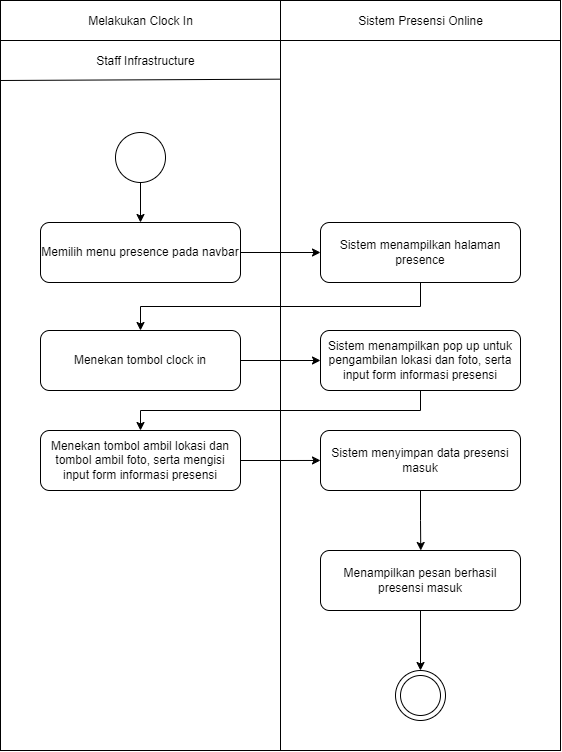
\includegraphics[width=17cm]{Gambar/bab2/activity-diagram-clock-in.png}
	\caption{\textit{Activity Diagram Clock In}}
	\label{fig:activity-diagram-clock-in}
\end{figure}
\FloatBarrier

\begin{figure}[H]
	\centering
	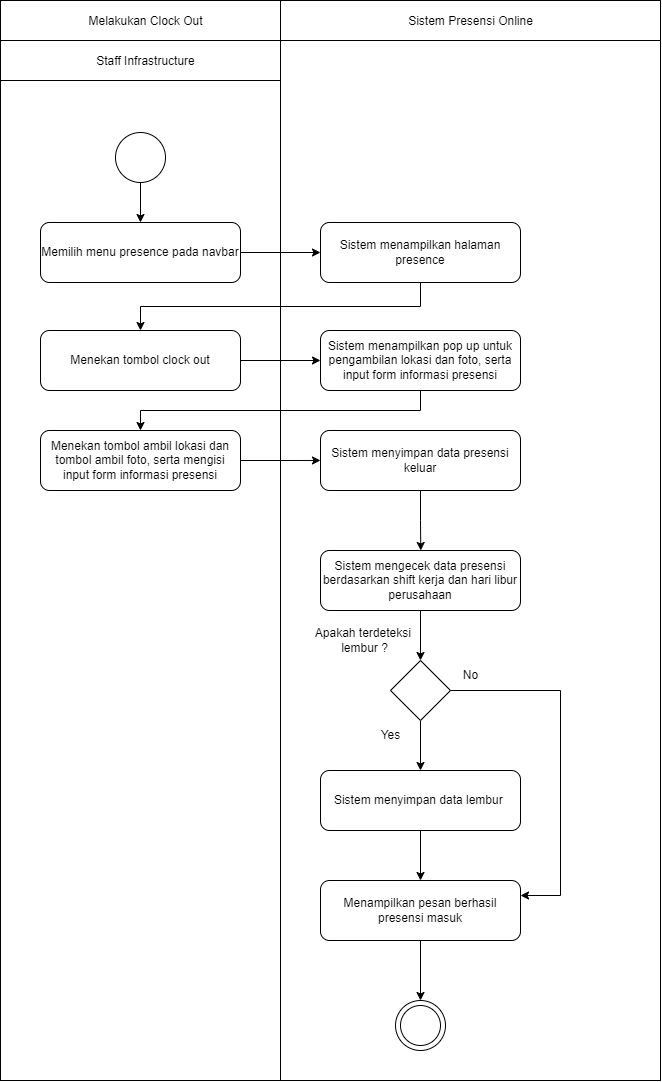
\includegraphics[width=13cm]{Gambar/bab2/activity-diagram-clock-out.png}
	\caption{\textit{Activity Diagram Clock Out}}
	\label{fig:activity-diagram-clock-out}
\end{figure}
\FloatBarrier

\begin{figure}[H]
	\centering
	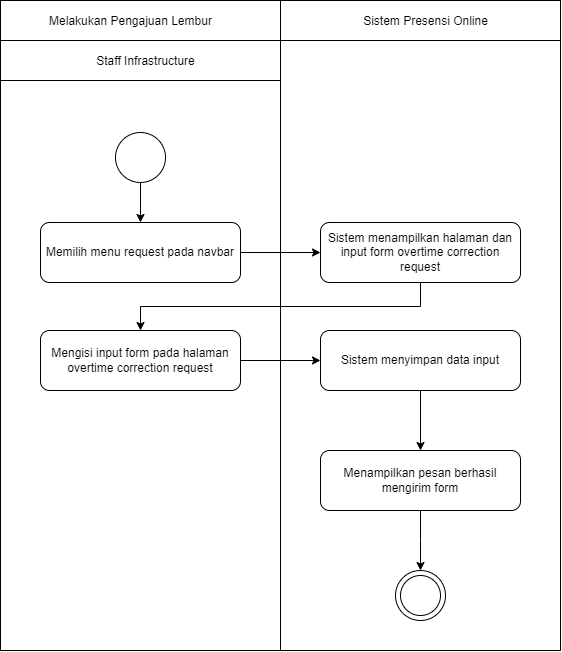
\includegraphics[width=15cm]{Gambar/bab2/activity-diagram-melakukan-pengajuan-lembur.png}
	\caption{\textit{Activity Diagram} Melakukan Pengajuan Lembur}
	\label{fig:activity-diagram-melakukan-pengajuan-lembur}
\end{figure}
\FloatBarrier

\begin{figure}[H]
	\centering
	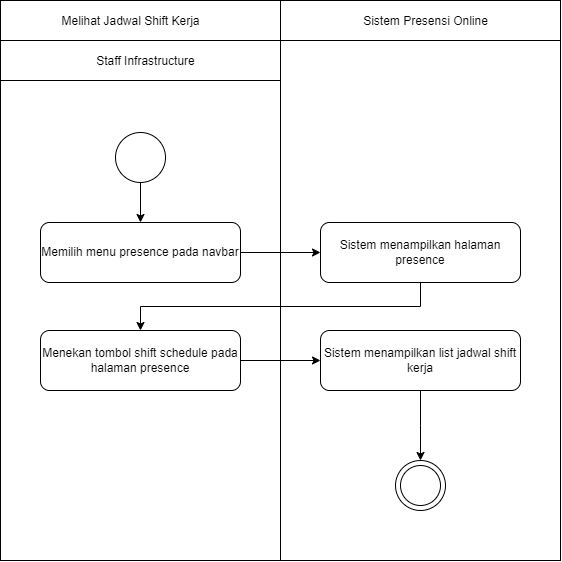
\includegraphics[width=15cm]{Gambar/bab2/activity-diagram-melihat-jadwal-shift-kerja.png}
	\caption{\textit{Activity Diagram} Melihat Jadwal \textit{Shift} Kerja}
	\label{fig:activity-diagram-melihat-jadwal-shift-kerja}
\end{figure}
\FloatBarrier

\begin{figure}[H]
	\centering
	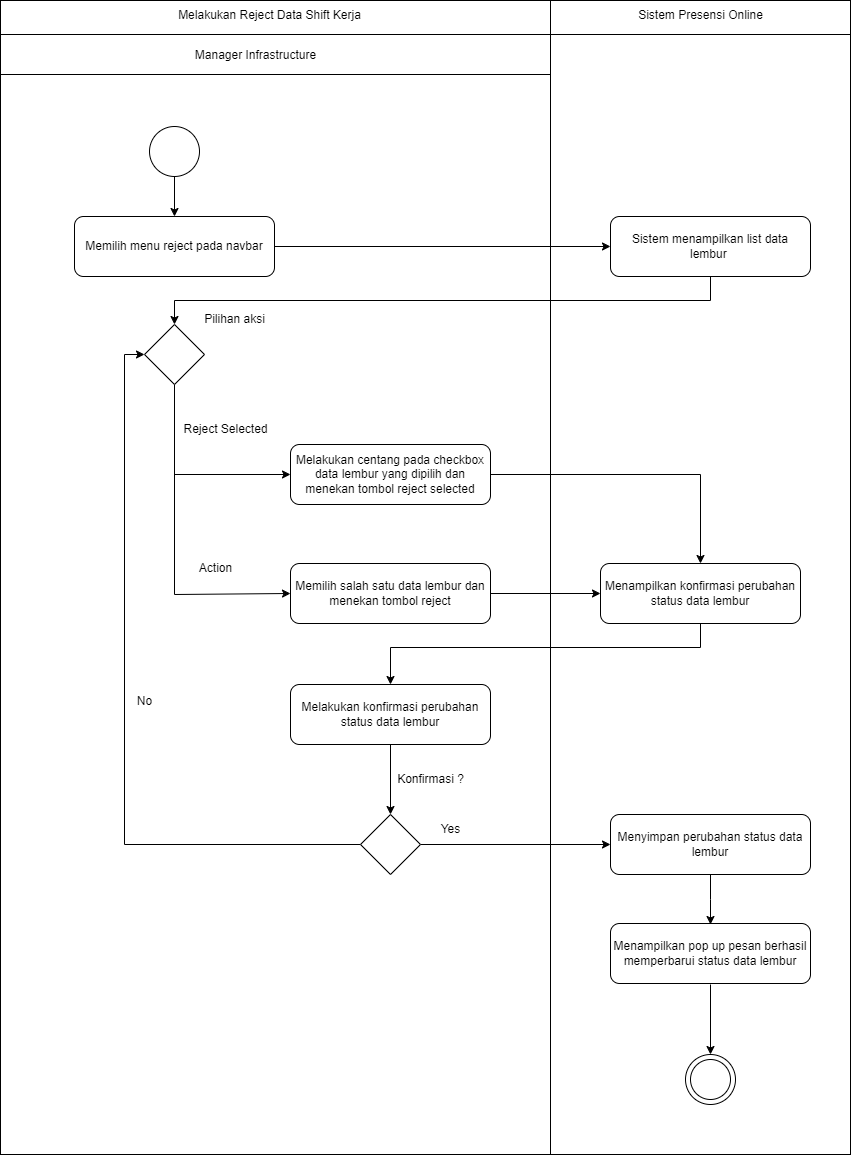
\includegraphics[width=14cm]{Gambar/bab2/activity-diagram-melakukan-reject.png}
	\caption{\textit{Activity Diagram} Melakukan \textit{Reject} pada Data Lembur}
	\label{fig:activity-diagram-melakukan-reject}
\end{figure}
\FloatBarrier

\begin{figure}[H]
	\centering
	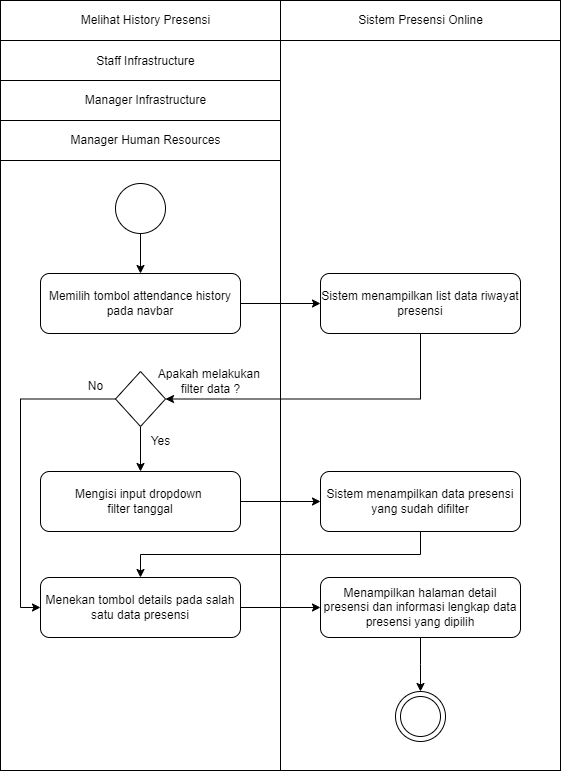
\includegraphics[width=15cm]{Gambar/bab2/activity-diagram-melihat-history-presensi.png}
	\caption{\textit{Activity Diagram} Melihat Riwayat Presensi}
	\label{fig:activity-diagram-melihat-riwayat-presensi}
\end{figure}
\FloatBarrier

\begin{figure}[H]
	\centering
	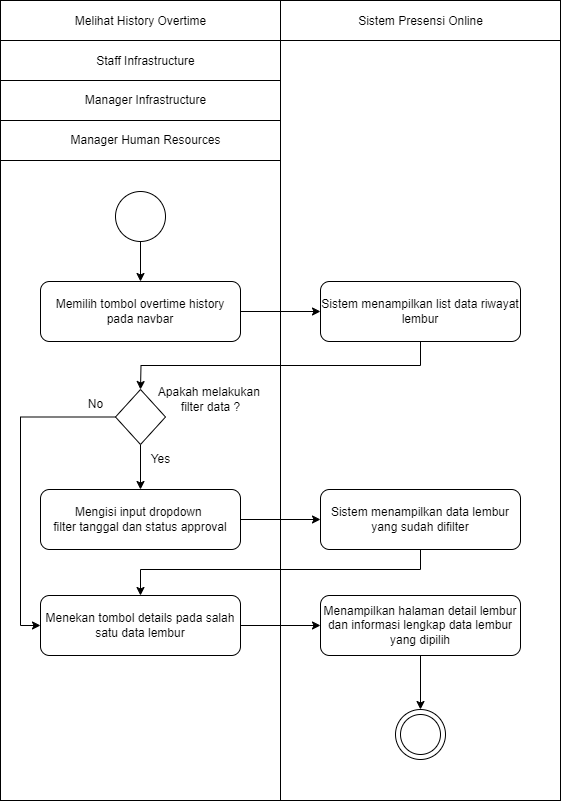
\includegraphics[width=15cm]{Gambar/bab2/activity-diagram-melihat-history-lembur.png}
	\caption{\textit{Activity Diagram} Melihat Riwayat Lembur}
	\label{fig:activity-diagram-melihat-riwayat-lembur}
\end{figure}
\FloatBarrier

\begin{figure}[H]
	\centering
	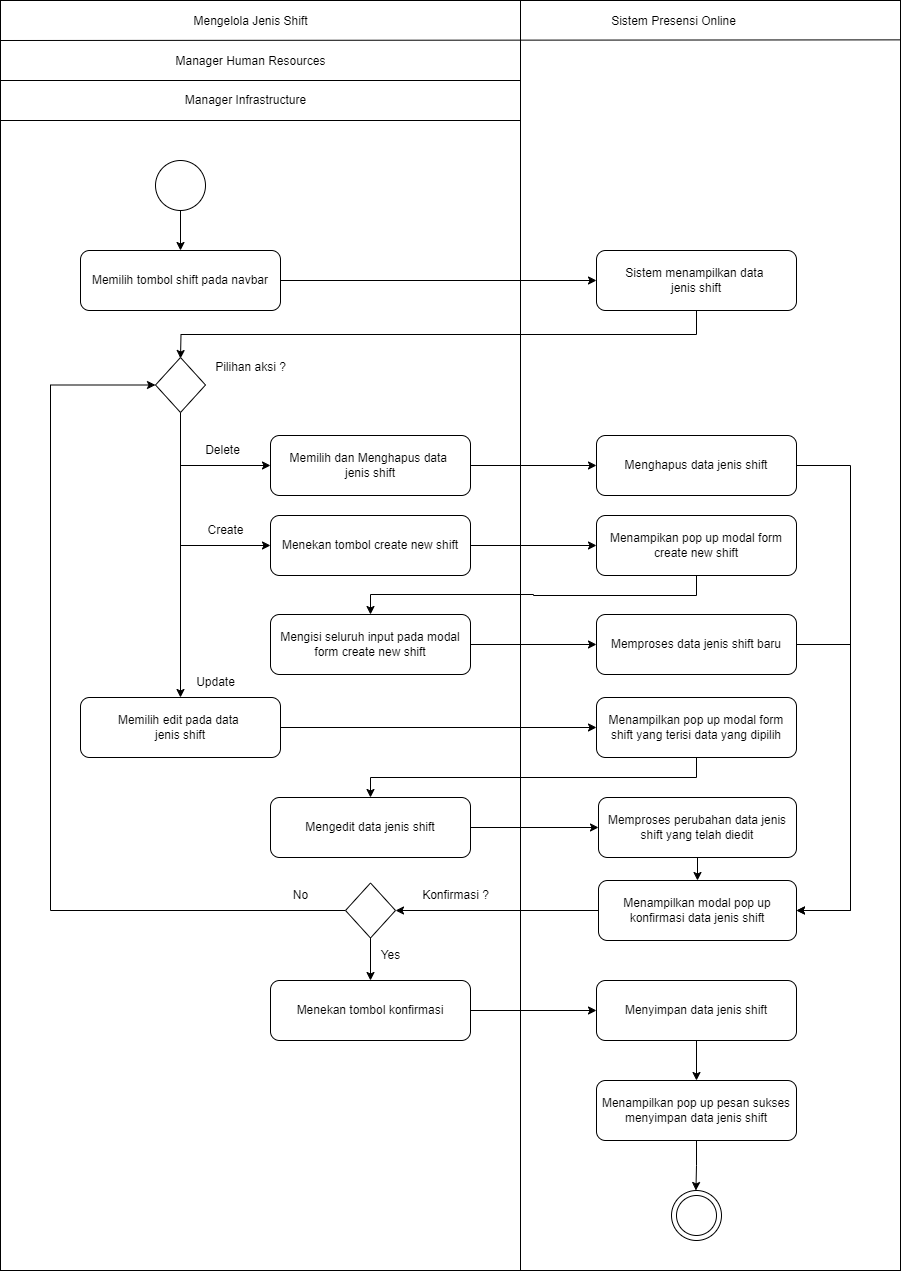
\includegraphics[width=15cm]{Gambar/bab2/activity-diagram-mengelola-data-jenis-shift.png}
	\caption{\textit{Activity Diagram} Mengelola Jenis \textit{Shift}}
	\label{fig:activity-diagram-mengelola-jenis-shift}
\end{figure}
\FloatBarrier

\begin{figure}[H]
	\centering
	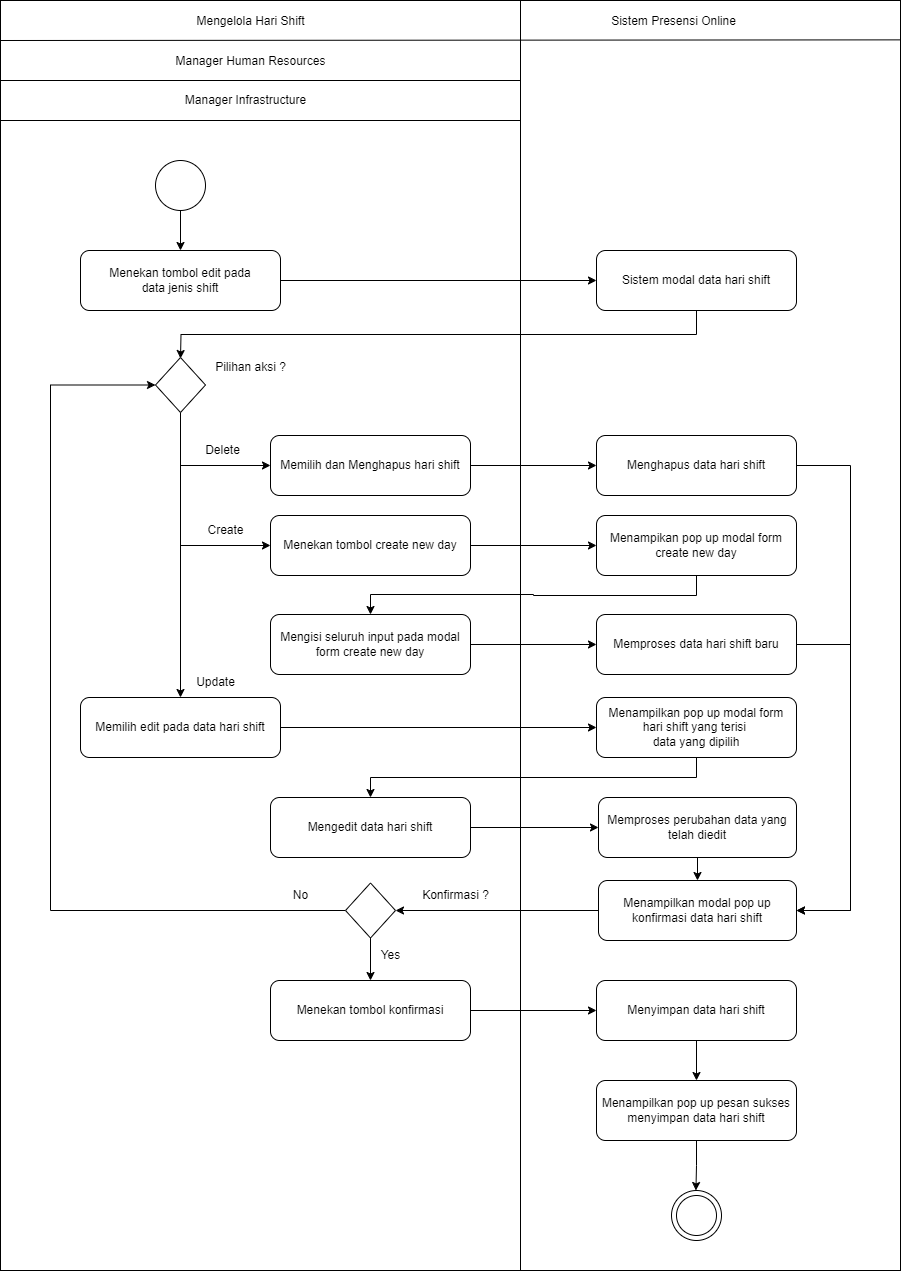
\includegraphics[width=15cm]{Gambar/bab2/activity-diagram-mengelola-data-hari-shift.png}
	\caption{\textit{Activity Diagram} Mengelola Hari \textit{Shift}}
	\label{fig:activity-diagram-mengelola-hari-shift}
\end{figure}
\FloatBarrier

\begin{figure}[H]
	\centering
	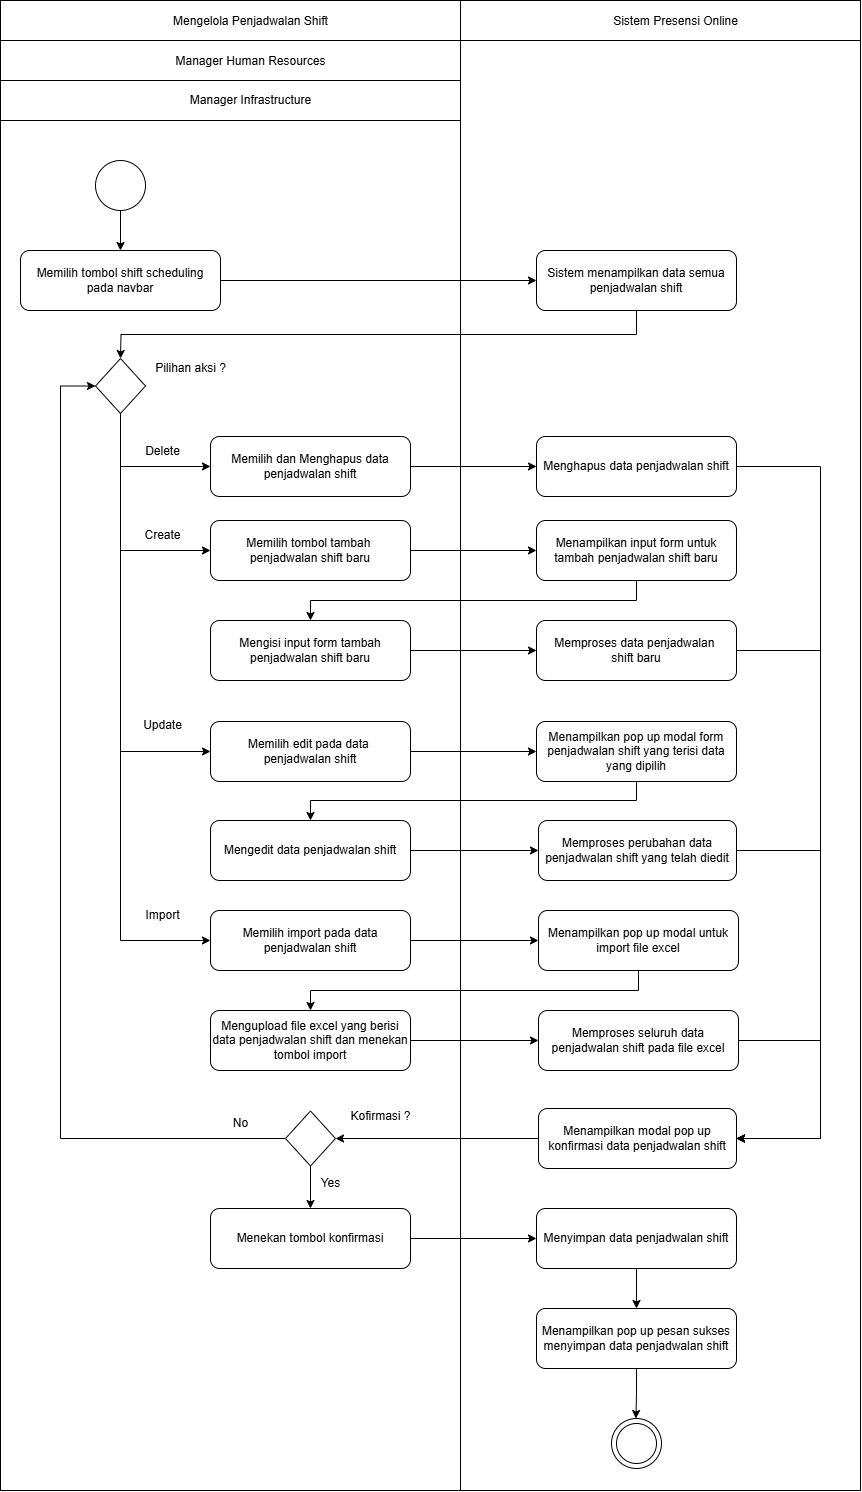
\includegraphics[width=13cm]{Gambar/bab2/activity-diagram-mengelola-penjadwalan-shift.png}
	\caption{\textit{Activity Diagram} Mengelola Penjadwalan \textit{Shift}}
	\label{fig:activity-diagram-mengelola-penjadwalan-shift}
\end{figure}
\FloatBarrier

\begin{figure}[H]
	\centering
	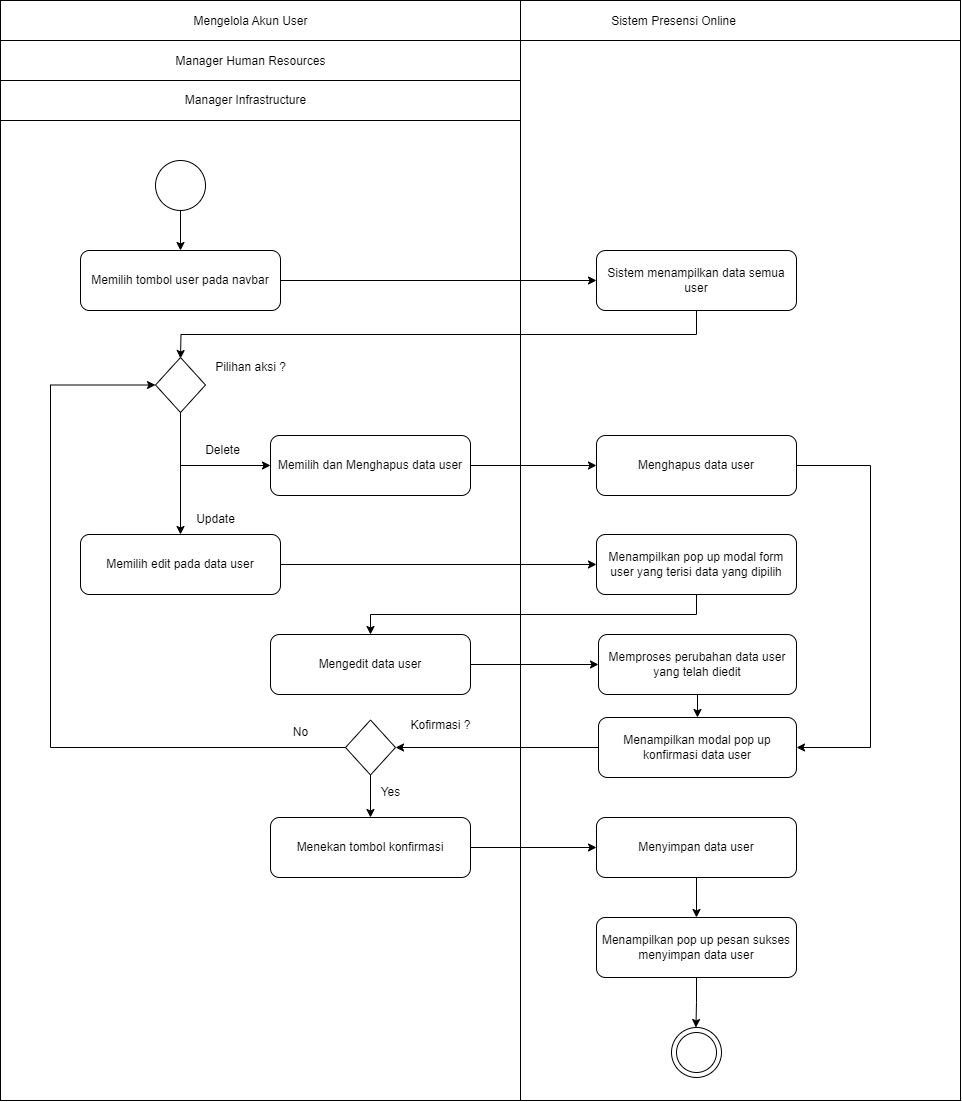
\includegraphics[width=15cm]{Gambar/bab2/activity-diagram-mengelola-data-user.png}
	\caption{\textit{Activity Diagram} Mengelola Akun \textit{User}}
	\label{fig:activity-diagram-mengelola-akun-user}
\end{figure}
\FloatBarrier

\begin{figure}[H]
	\centering
	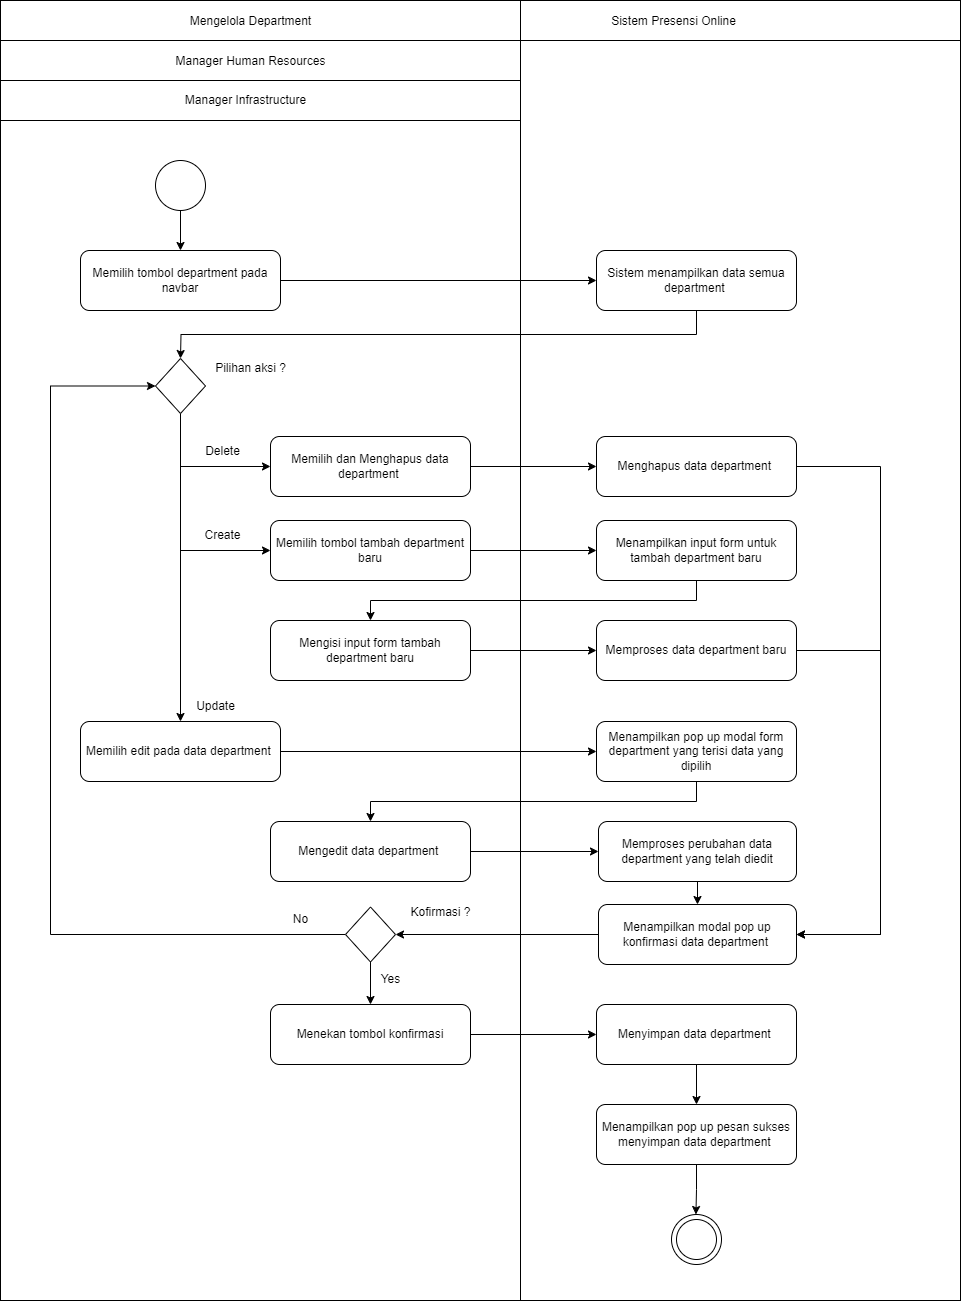
\includegraphics[width=15cm]{Gambar/bab2/activity-diagram-mengelola-data-department.png}
	\caption{\textit{Activity Diagram} Mengelola \textit{Department}}
	\label{fig:activity-diagram-mengelola-department}
\end{figure}
\FloatBarrier

\begin{figure}[H]
	\centering
	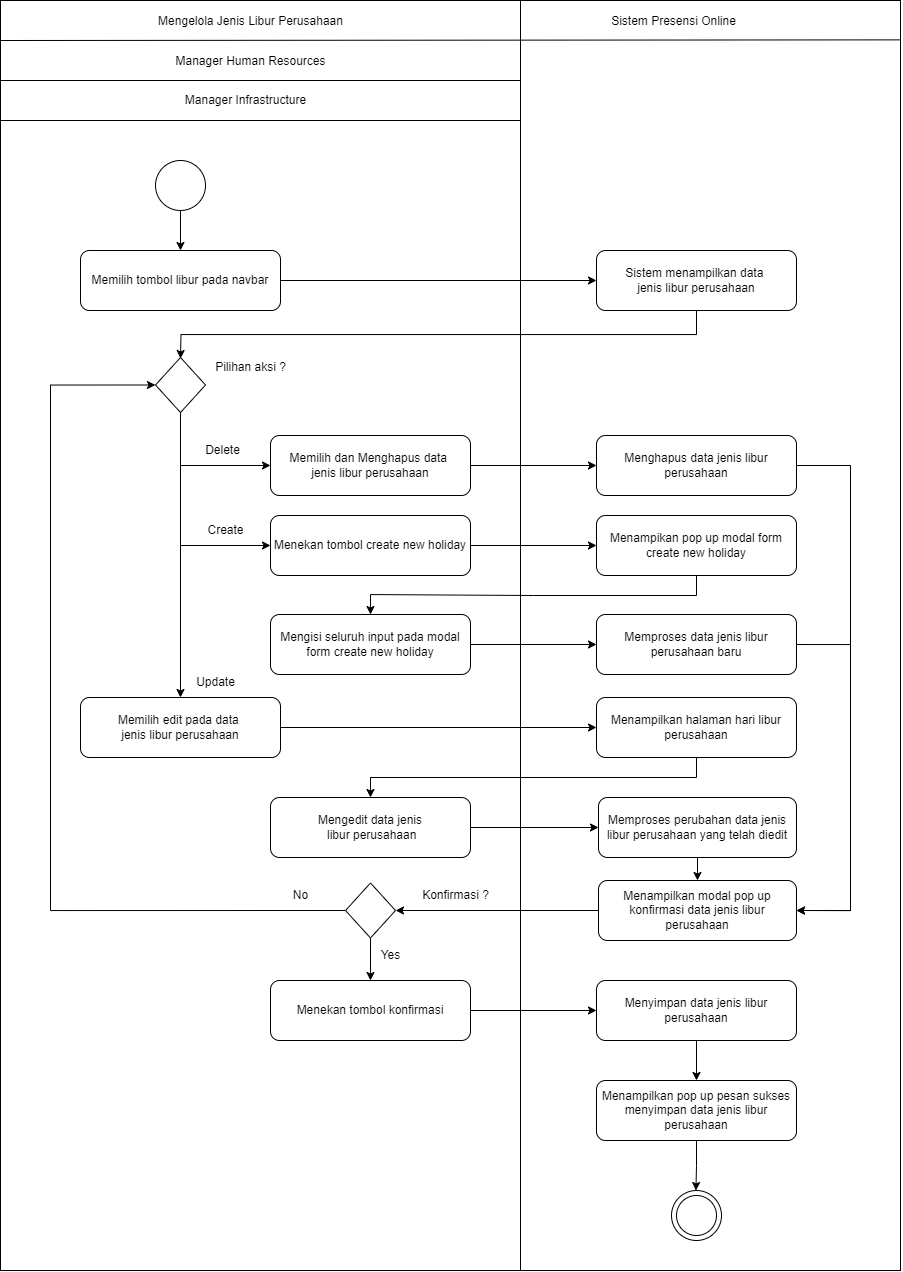
\includegraphics[width=13cm]{Gambar/bab2/activity-diagram-mengelola-data-jenis-libur-perusahaan.png}
	\caption{\textit{Activity Diagram} Mengelola Data Jenis Libur Perusahaan}
	\label{fig:activity-diagram-mengelola-data-jenis-libur-perusahaan}
\end{figure}
\FloatBarrier

\begin{figure}[H]
	\centering
	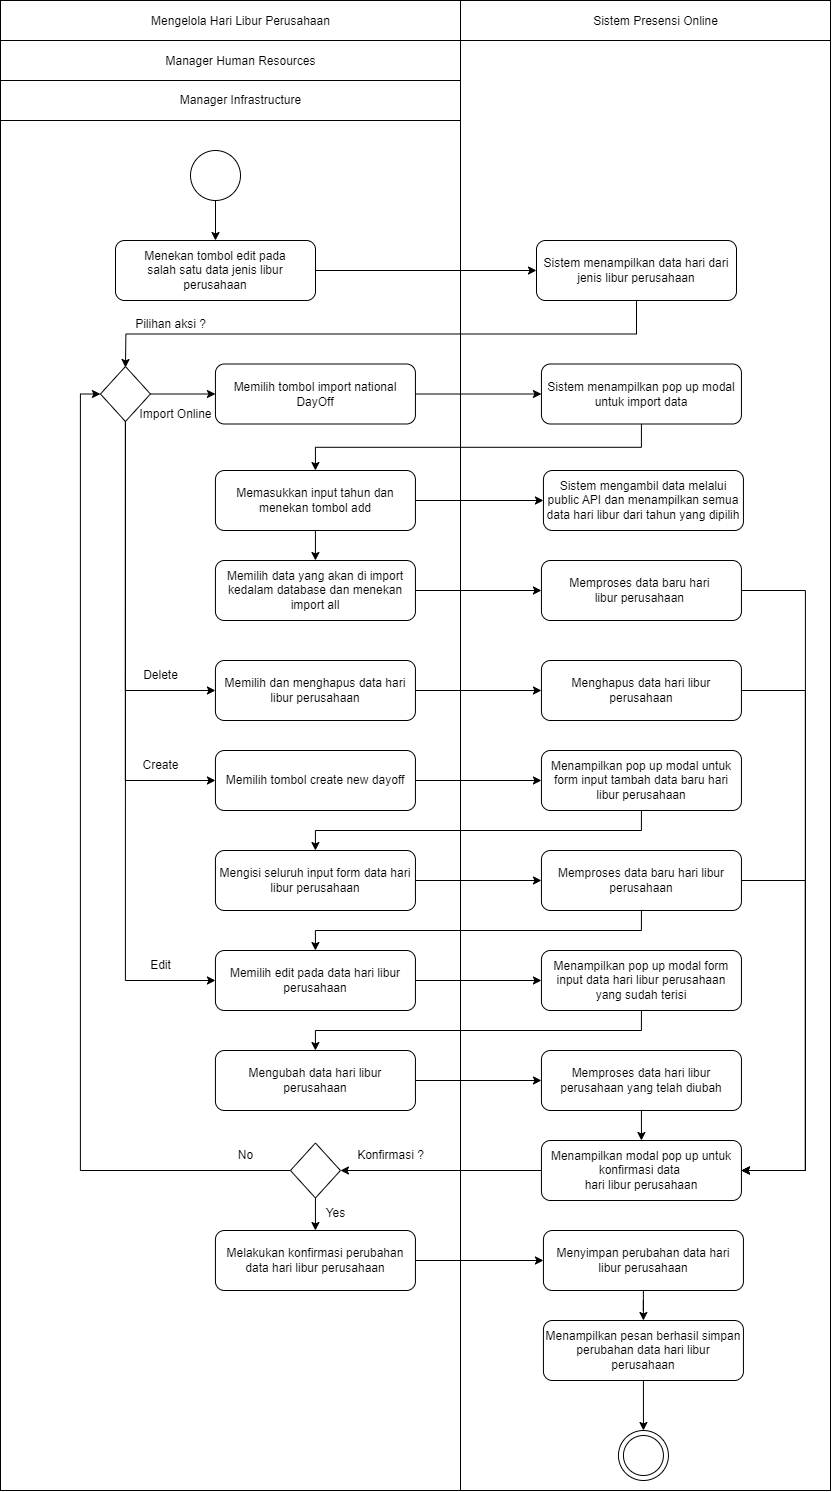
\includegraphics[width=13cm]{Gambar/bab2/activity-diagram-mengelola-data-hari-libur-perusahaan.png}
	\caption{\textit{Activity Diagram} Mengelola Data Hari Libur Perusahaan}
	\label{fig:activity-diagram-mengelola-data-hari-libur-perusahaan}
\end{figure}
\FloatBarrier

\begin{figure}[H]
	\centering
	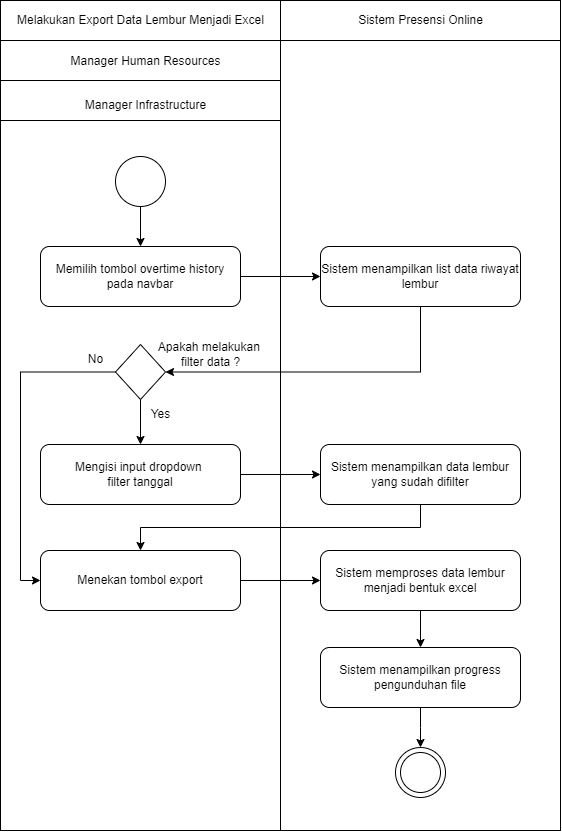
\includegraphics[width=15cm]{Gambar/bab2/activity-diagram-melakukan-export-data-lembur.png}
	\caption{\textit{Activity Diagram} Melakukan \textit{Export} Data Lembur ke \textit{Excel}}
	\label{fig:activity-diagram-melakukan-export-data-lembur-ke-excel}
\end{figure}
\FloatBarrier

\begin{figure}[H]
	\centering
	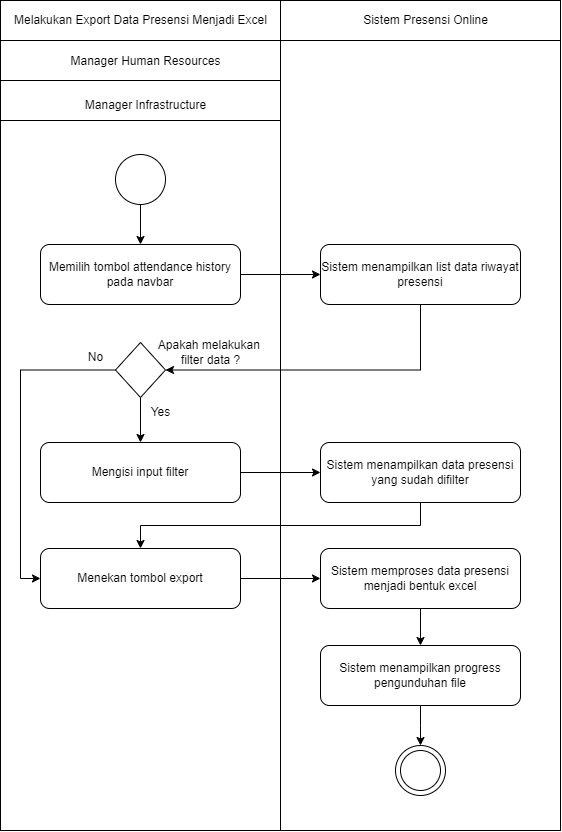
\includegraphics[width=15cm]{Gambar/bab2/activity-diagram-melakukan-export-data-presensi.png}
	\caption{\textit{Activity Diagram} Melakukan \textit{Export} Data Presensi ke \textit{Excel}}
	\label{fig:activity-diagram-melakukan-export-data-presensi-ke-excel}
\end{figure}
\FloatBarrier

\pagebreak

\nextappendix
\section*{Lampiran \theappendixletter: \textit{Sequence Diagram} Aplikasi Presensi \textit{Online} 
\label{sec:sequence-diagram-aplikasi-presensi-online}}
\addcontentsline{toc}{section}{Lampiran \theappendixletter: \textit{Sequence Diagram} Aplikasi Presensi \textit{Online}}
\begin{figure}[H]
	\centering
	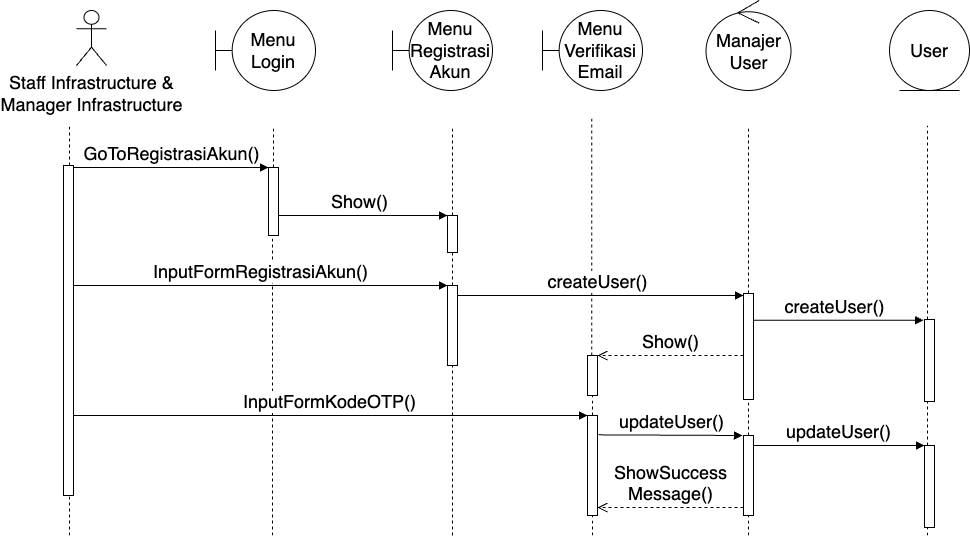
\includegraphics[width=15cm]{Gambar/bab2/sequence-diagram-registrasi-akun.png}
	\caption{\textit{Sequence Diagram} Registrasi Akun}
	\label{fig:sequence-diagram-registrasi-akun}
\end{figure}
\FloatBarrier

\begin{figure}[H]
	\centering
	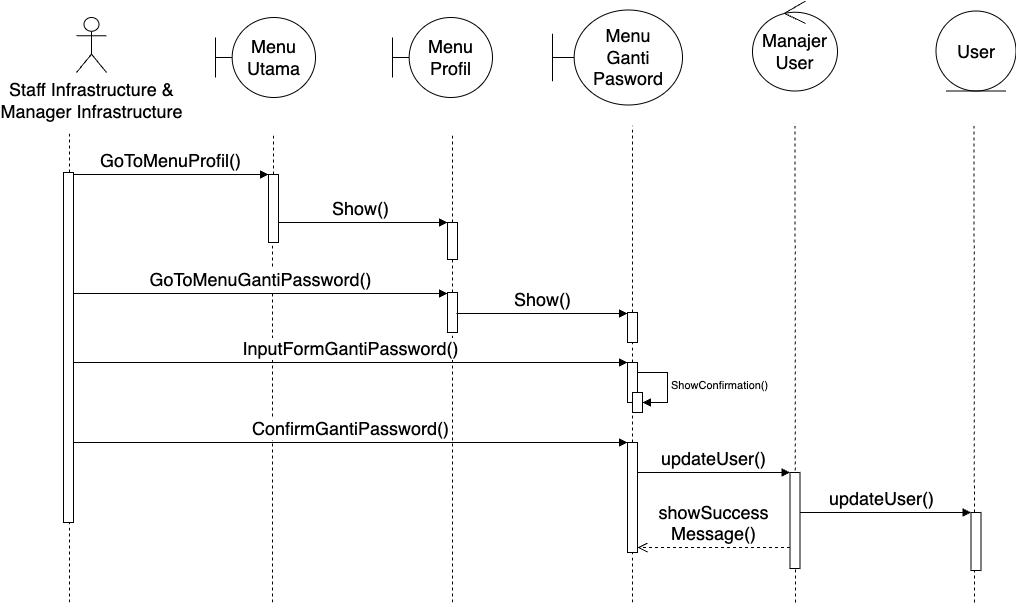
\includegraphics[width=15cm]{Gambar/bab2/sequence-diagram-ganti-password.png}
	\caption{\textit{Sequence Diagram} Ganti Password}
	\label{fig:sequence-diagram-ganti-password}
\end{figure}
\FloatBarrier

\begin{figure}[H]
	\centering
	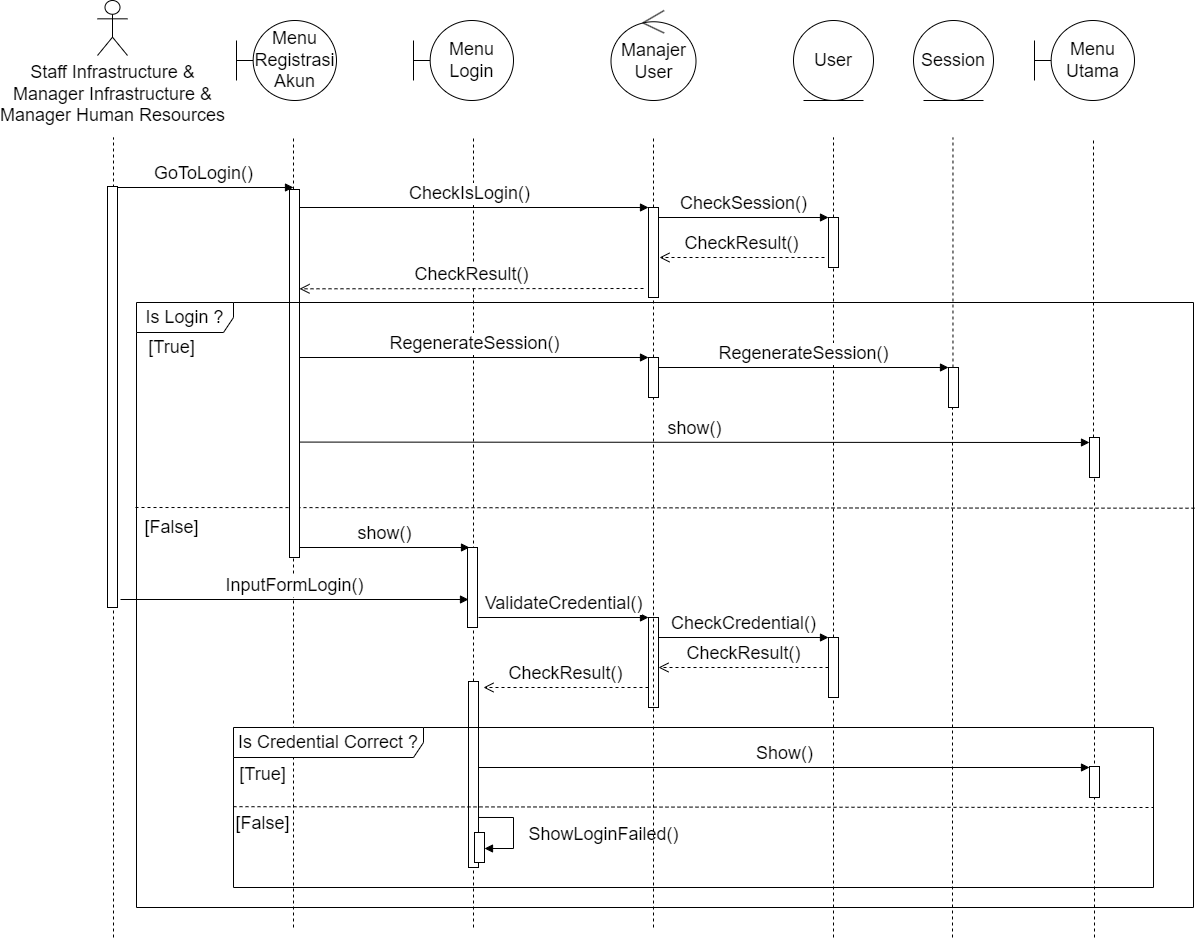
\includegraphics[width=17cm]{Gambar/bab2/sequence-diagram-login.png}
	\caption{\textit{Sequence Diagram Login}}
	\label{fig:sequence-diagram-login}
\end{figure}
\FloatBarrier

\begin{figure}[H]
	\centering
	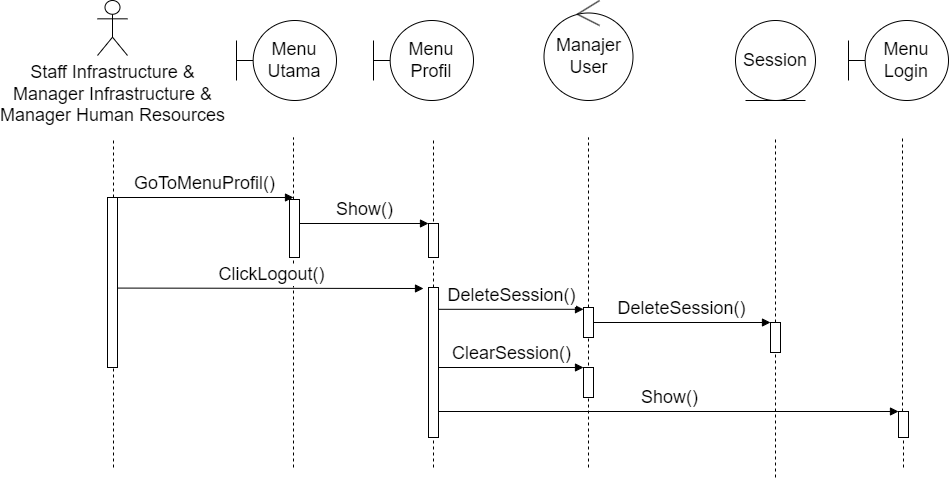
\includegraphics[width=17cm]{Gambar/bab2/sequence-diagram-logout.png}
	\caption{\textit{Sequence Diagram Logout}}
	\label{fig:sequence-diagram-logout}
\end{figure}
\FloatBarrier

\begin{figure}[H]
	\centering
	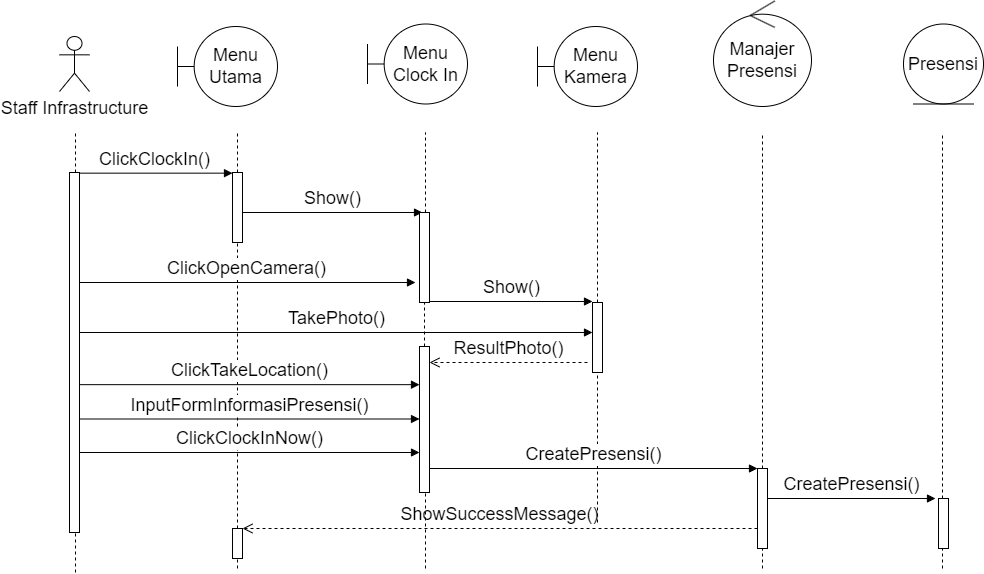
\includegraphics[width=17cm]{Gambar/bab2/sequence-diagram-clock-in.png}
	\caption{\textit{Sequence Diagram Clock In}}
	\label{fig:sequence-diagram-clock-in}
\end{figure}
\FloatBarrier

\begin{figure}[H]
	\centering
	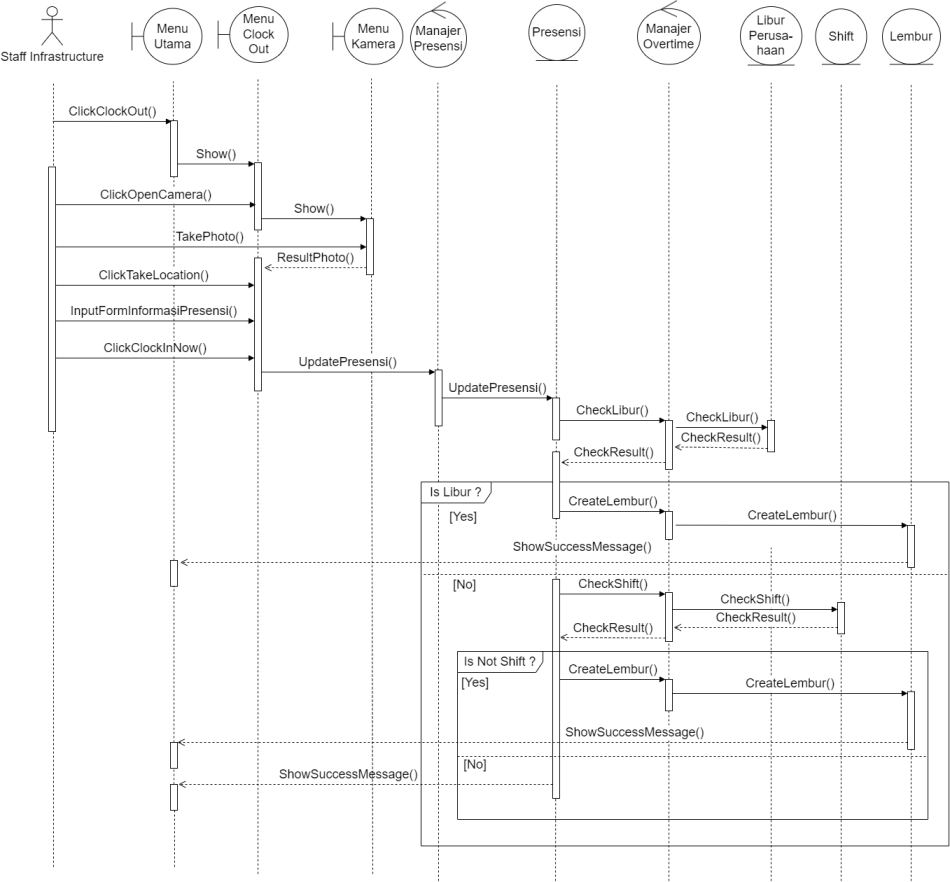
\includegraphics[width=18cm]{Gambar/bab2/sequence-diagram-clock-out.png}
	\caption{\textit{Sequence Diagram Clock Out}}
	\label{fig:sequence-diagram-clock-out}
\end{figure}
\FloatBarrier

\begin{figure}[H]
	\centering
	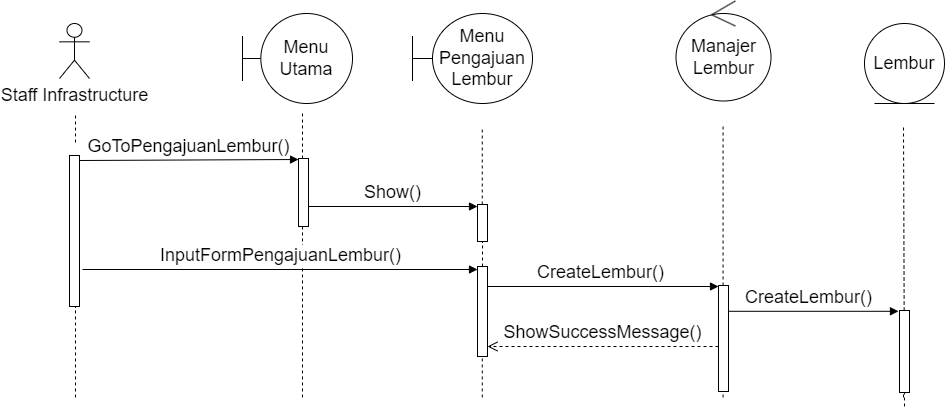
\includegraphics[width=17cm]{Gambar/bab2/sequence-diagram-melakukan-pengajuan-lembur.png}
	\caption{\textit{Sequence Diagram} Melakukan Pengajuan Lembur}
	\label{fig:sequence-diagram-melakukan-pengajuan-lembur}
\end{figure}
\FloatBarrier

\begin{figure}[H]
	\centering
	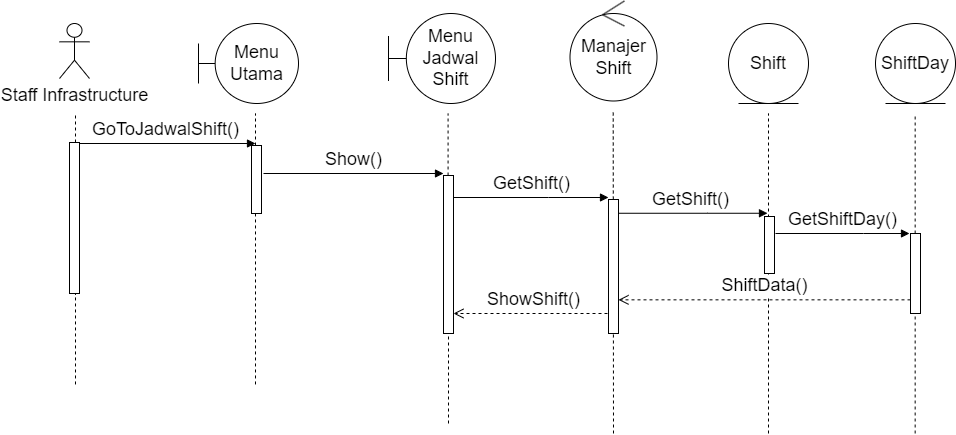
\includegraphics[width=17cm]{Gambar/bab2/sequence-diagram-melihat-jadwal-shift.png}
	\caption{\textit{Sequence Diagram} Melihat Jadwal \textit{Shift} Kerja}
	\label{fig:sequence-diagram-melihat-jadwal-shift-kerja}
\end{figure}
\FloatBarrier

\begin{figure}[H]
	\centering
	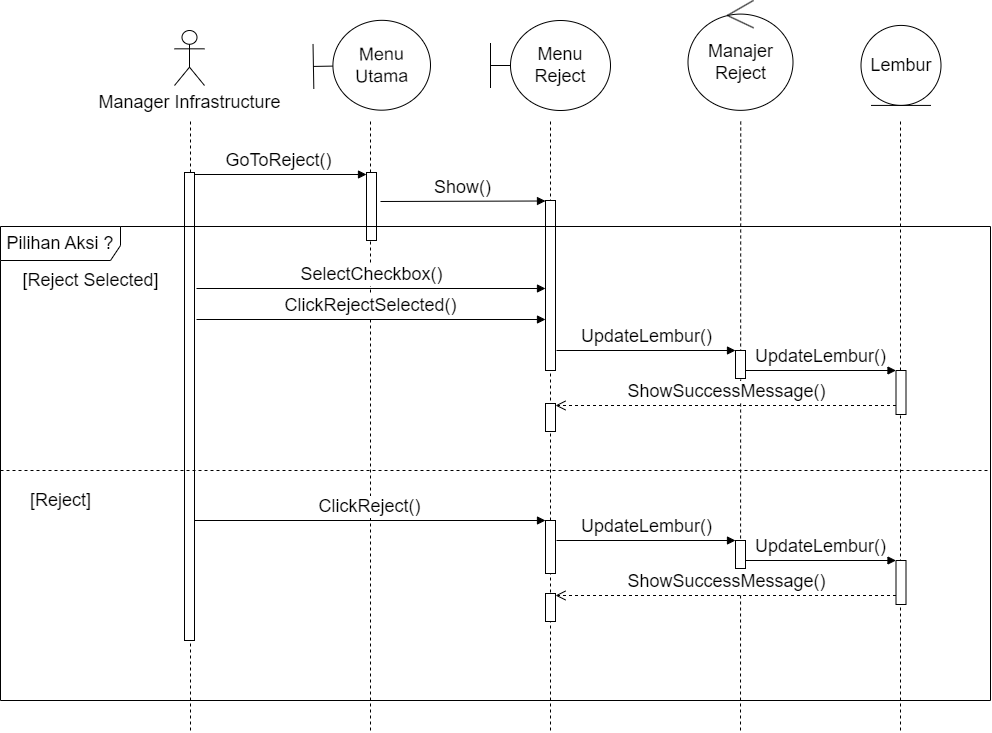
\includegraphics[width=17cm]{Gambar/bab2/sequence-diagram-melakukan-reject.png}
	\caption{\textit{Sequence Diagram} Melakukan \textit{Reject} pada Data Lembur}
	\label{fig:sequence-diagram-melakukan-reject-pada-data-lembur}
\end{figure}
\FloatBarrier

\begin{figure}[H]
	\centering
	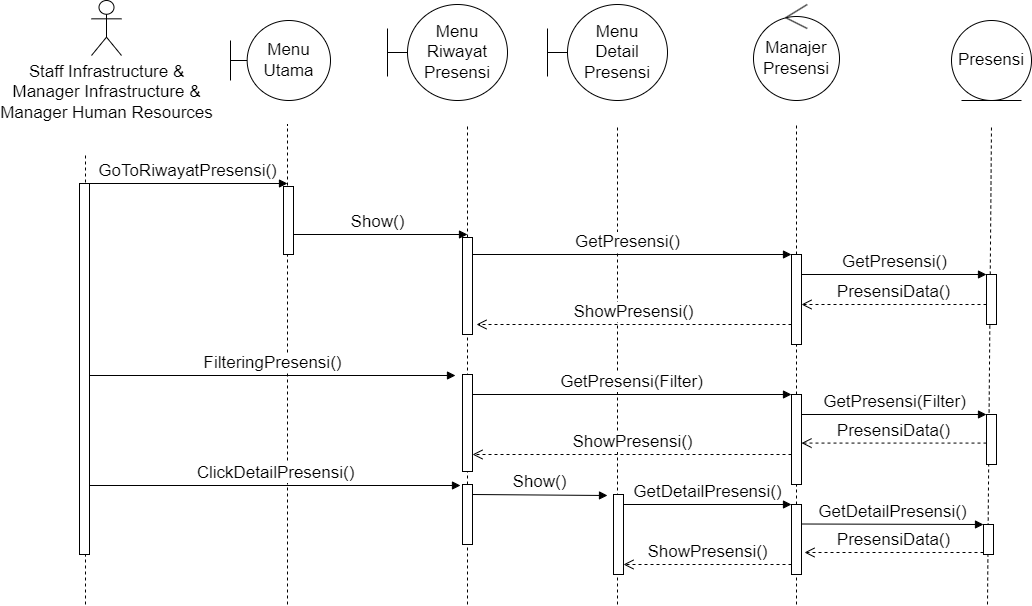
\includegraphics[width=17cm]{Gambar/bab2/sequence-diagram-melihat-riwayat-presensi.png}
	\caption{\textit{Sequence Diagram} Melihat Riwayat Presensi}
	\label{fig:sequence-diagram-melihat-riwayat-presensi}
\end{figure}
\FloatBarrier

\begin{figure}[H]
	\centering
	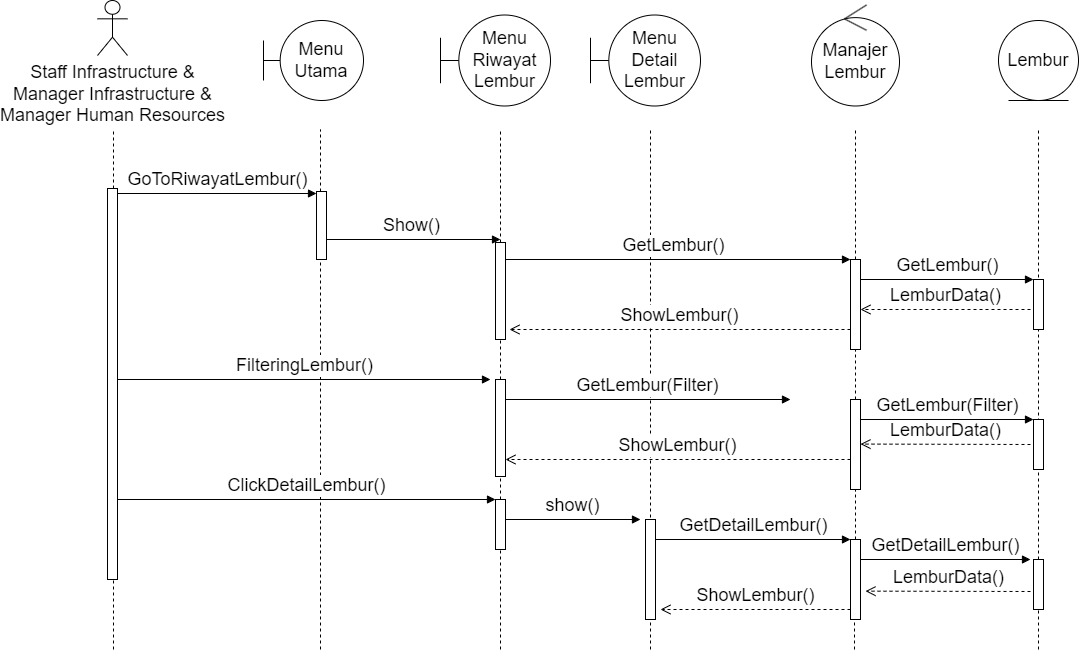
\includegraphics[width=17cm]{Gambar/bab2/sequence-diagram-melihat-riwayat-lembur.png}
	\caption{\textit{Sequence Diagram} Melihat Riwayat Lembur}
	\label{fig:sequence-diagram-melihat-riwayat-lembur}
\end{figure}
\FloatBarrier

\begin{figure}[H]
	\centering
	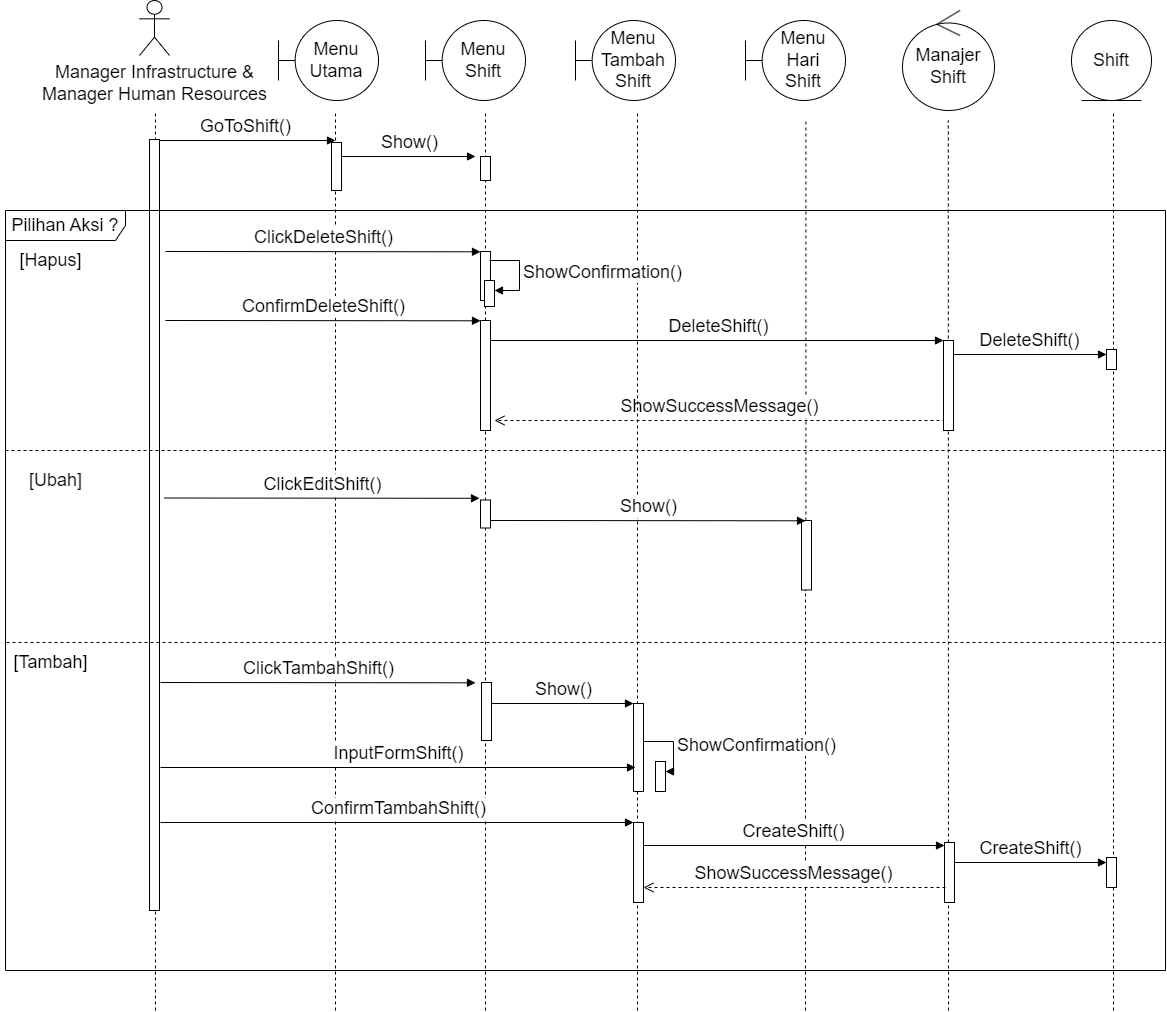
\includegraphics[width=18cm]{Gambar/bab2/sequence-diagram-mengelola-data-jenis-shift.png}
	\caption{\textit{Sequence Diagram} Mengelola Jenis \textit{Shift}}
	\label{fig:sequence-diagram-mengelola-jenis-shift}
\end{figure}
\FloatBarrier

\begin{figure}[H]
	\centering
	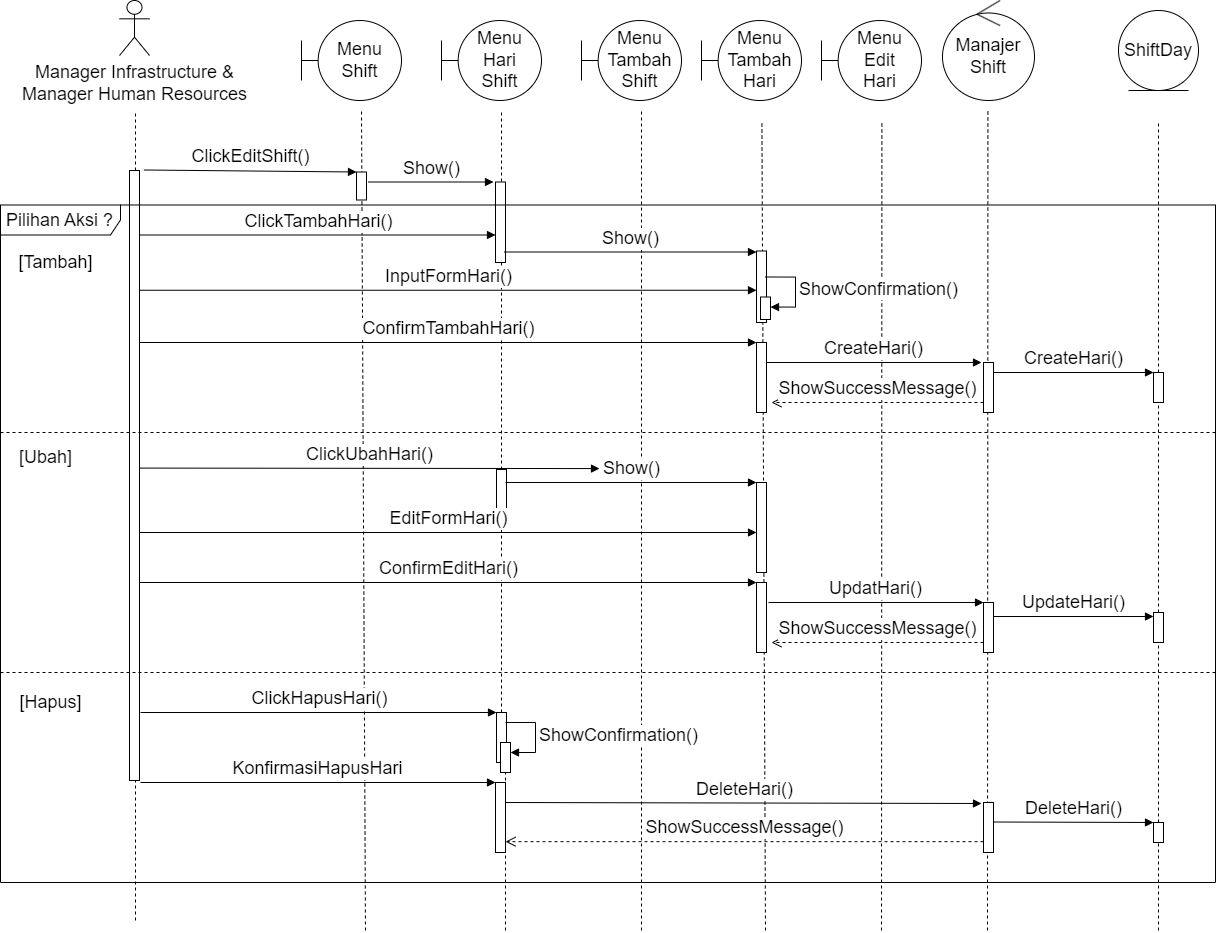
\includegraphics[width=18cm]{Gambar/bab2/sequence-diagram-mengelola-data-hari-shift.png}
	\caption{\textit{Sequence Diagram} Mengelola Hari \textit{Shift}}
	\label{fig:sequence-diagram-mengelola-hari-shift}
\end{figure}
\FloatBarrier

\begin{figure}[H]
	\centering
	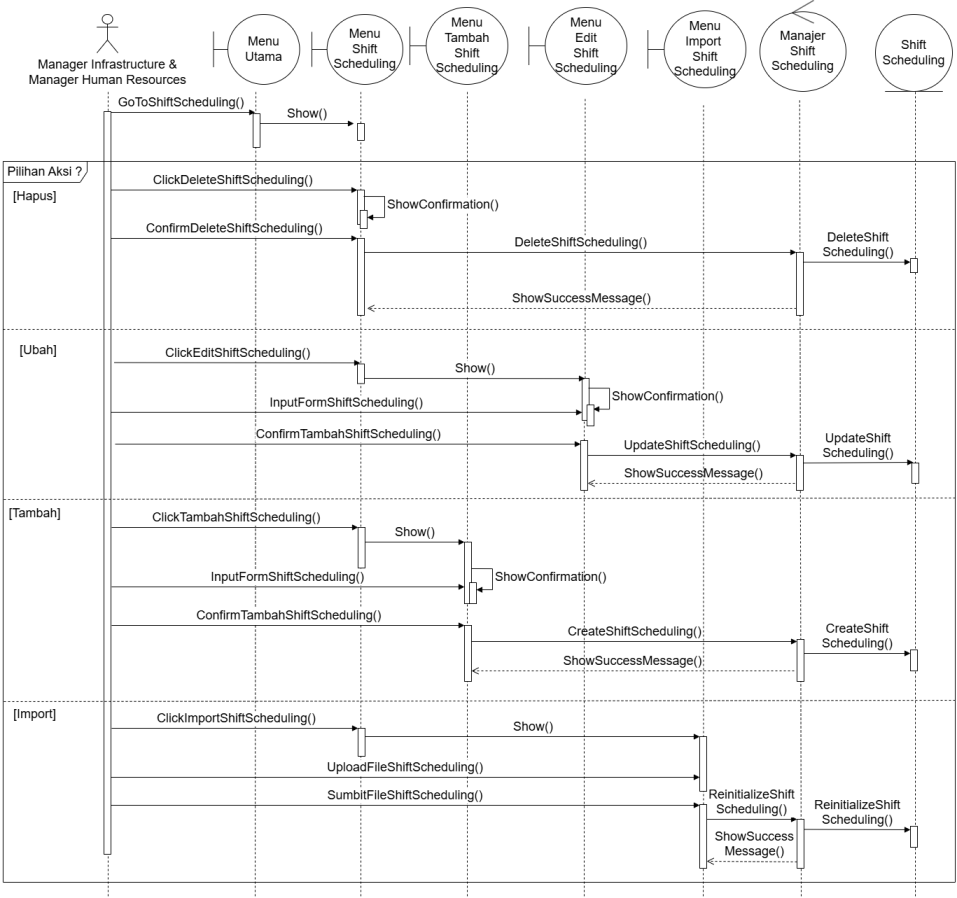
\includegraphics[width=18cm]{Gambar/bab2/sequence-diagram-mengelola-data-penjadwalan-shift.png}
	\caption{\textit{Sequence Diagram} Mengelola Penjadwalan \textit{Shift}}
	\label{fig:sequence-diagram-mengelola-penjadwalan-shift}
\end{figure}
\FloatBarrier

\begin{figure}[H]
	\centering
	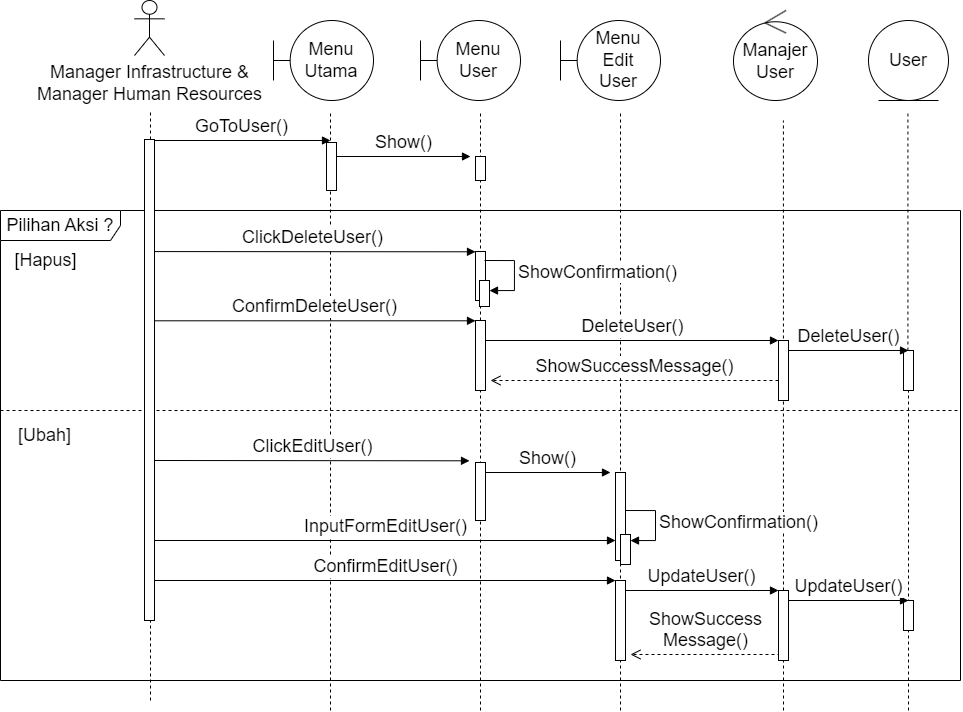
\includegraphics[width=15cm]{Gambar/bab2/sequence-diagram-mengelola-akun-user.png}
	\caption{\textit{Sequence Diagram} Mengelola Akun \textit{User}}
	\label{fig:sequence-diagram-mengelola-akun-user}
\end{figure}
\FloatBarrier

\begin{figure}[H]
	\centering
	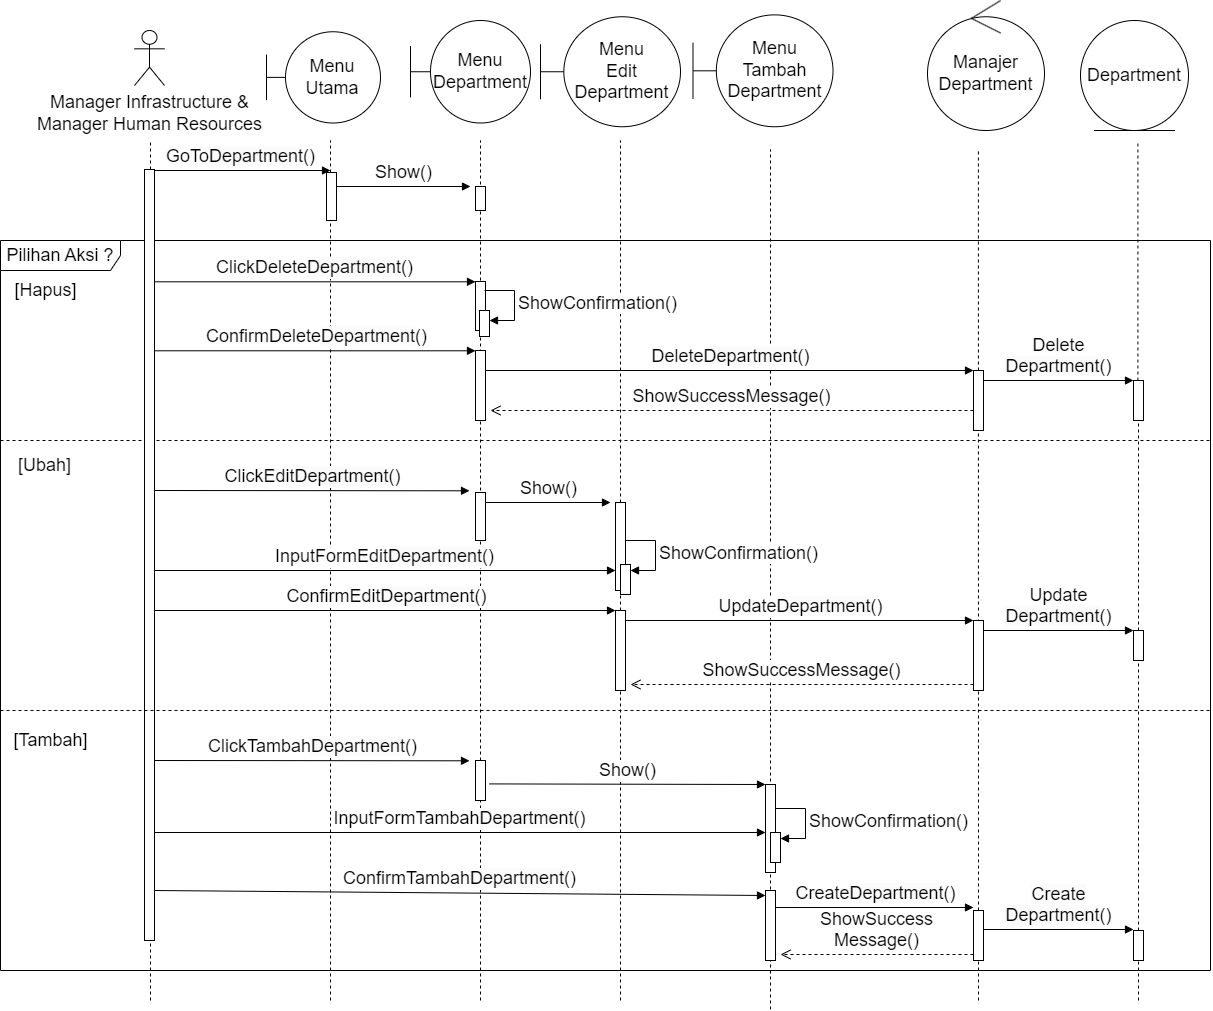
\includegraphics[width=15cm]{Gambar/bab2/sequence-diagram-mengelola-department.png}
	\caption{\textit{Sequence Diagram} Mengelola \textit{Department}}
	\label{fig:sequence-diagram-mengelola-department}
\end{figure}
\FloatBarrier

\begin{figure}[H]
	\centering
	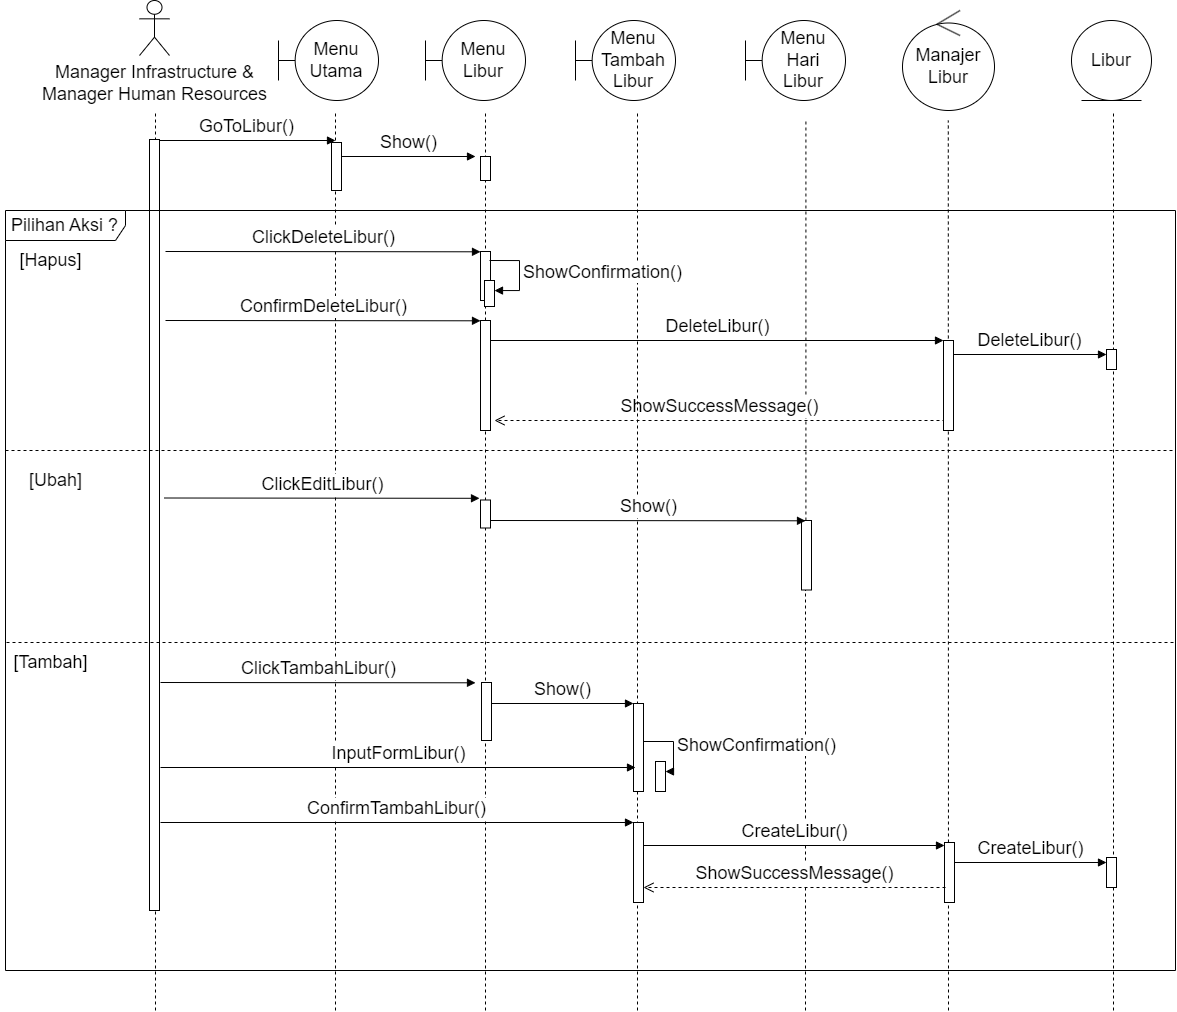
\includegraphics[width=15cm]{Gambar/bab2/sequence-diagram-mengelola-data-jenis-libur.png}
	\caption{\textit{Sequence Diagram} Mengelola Data Jenis Libur Perusahaan}
	\label{fig:sequence-diagram-mengelola-data-jenis-libur-perusahaan}
\end{figure}
\FloatBarrier

\begin{figure}[H]
	\centering
	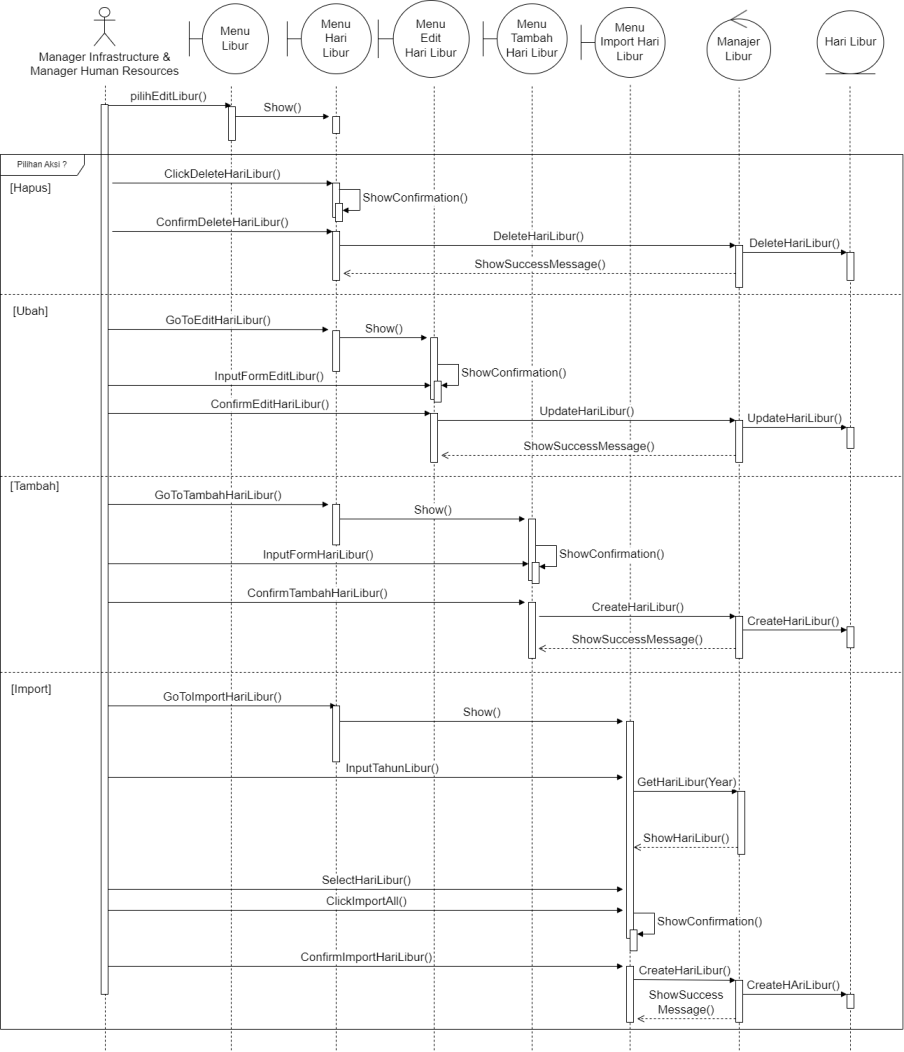
\includegraphics[width=15cm]{Gambar/bab2/sequence-diagram-mengelola-data-hari-libur.png}
	\caption{\textit{Sequence Diagram} Mengelola Data Hari Libur Perusahaan}
	\label{fig:sequence-diagram-mengelola-data-hari-libur-perusahaan}
\end{figure}
\FloatBarrier

\begin{figure}[H]
	\centering
	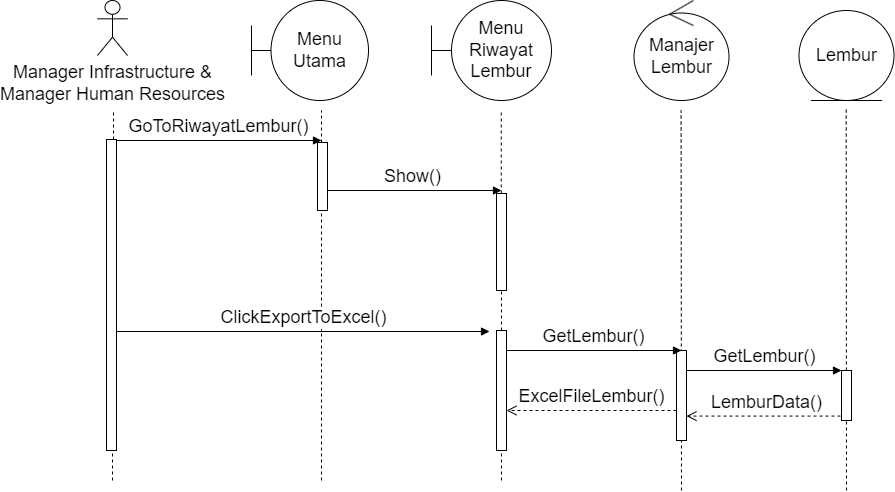
\includegraphics[width=15cm]{Gambar/bab2/sequence-diagram-melakukan-export-data-lembur-ke-excel.png}
	\caption{\textit{Sequence Diagram} melakukan \textit{Export} Data Lembur ke \textit{Excel}}
	\label{fig:sequence-diagram-melakukan-export-data-lembur-ke-excel}
\end{figure}
\FloatBarrier

\begin{figure}[H]
	\centering
	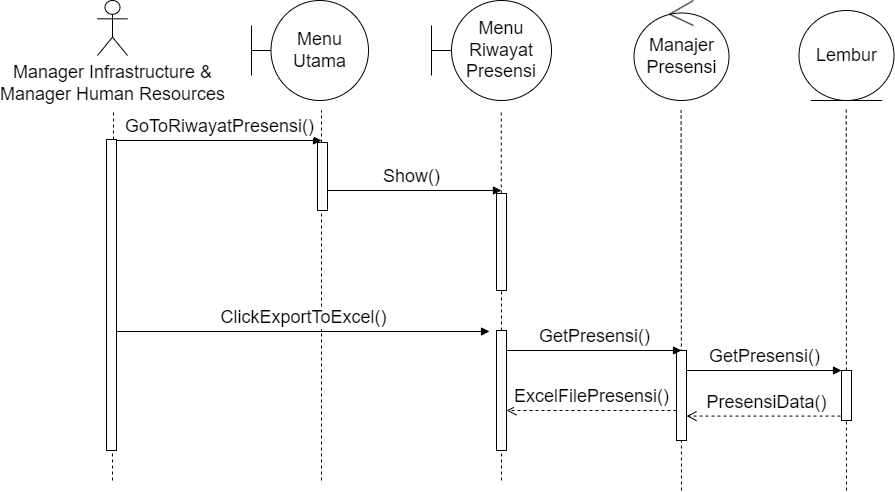
\includegraphics[width=15cm]{Gambar/bab2/sequence-diagram-melakukan-export-data-presensi-ke-excel.png}
	\caption{\textit{Sequence Diagram} melakukan \textit{Export} Data Presensi ke \textit{Excel}}
	\label{fig:sequence-diagram-melakukan-export-data-presensi-ke-excel}
\end{figure}
\FloatBarrier
\pagebreak


\begin{landscape}
\nextappendix
\section*{Lampiran \theappendixletter: \textit{Class Diagram} Aplikasi Presensi \textit{Online}}
\label{sec:class-diagram-aplikasi-presensi-online}
\addcontentsline{toc}{section}{Lampiran \theappendixletter: \textit{Class Diagram} Aplikasi Presensi \textit{Online}}
\begin{figure}[H]
	\centering
	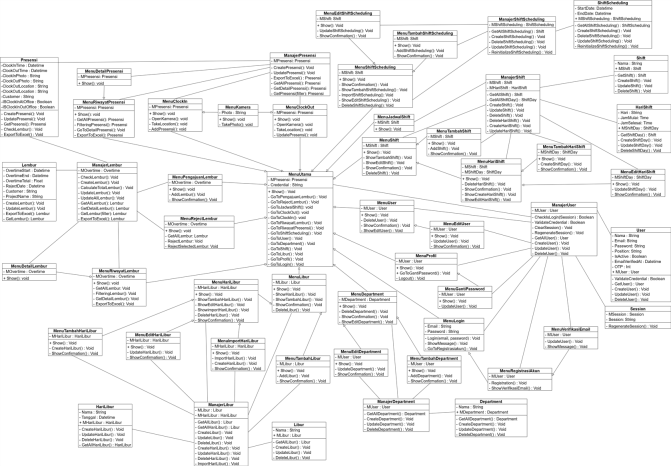
\includegraphics[width=21cm]{Gambar/bab2/class-diagram.png}
	\caption{\textit{Class Diagram} Aplikasi Presensi \textit{Online}}
	\label{fig:class-diagram-aplikasi-presensi-online}
\end{figure}
\end{landscape}

\nextappendix
\section*{Lampiran \theappendixletter: \textit{Conceptual Data Modeling}}
\label{sec:conceptual-database-design}
\addcontentsline{toc}{section}{Lampiran \theappendixletter: \textit{Conceptual Data Modeling}}
\begin{figure}[H]
	\centering
	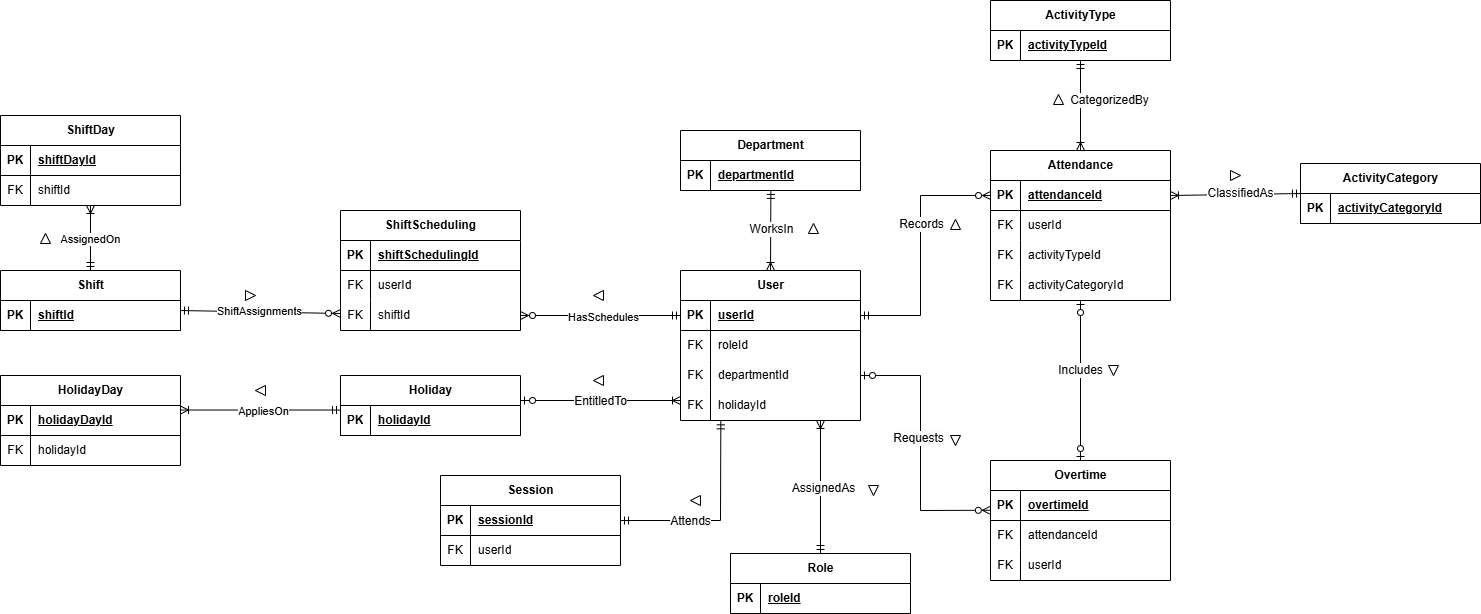
\includegraphics[width=17cm]{Gambar/bab2/conceptual-database-design.png}
	\caption{\textit{Conceptual Data Modeling}}
	\label{fig:conceptual-database-design}
\end{figure}

\nextappendix
\section*{Lampiran \theappendixletter: \textit{Logical Data Modeling}}
\label{sec:logical-database-design}
\addcontentsline{toc}{section}{Lampiran \theappendixletter: \textit{Logical Data Modeling}}
\begin{figure}[H]
	\centering
	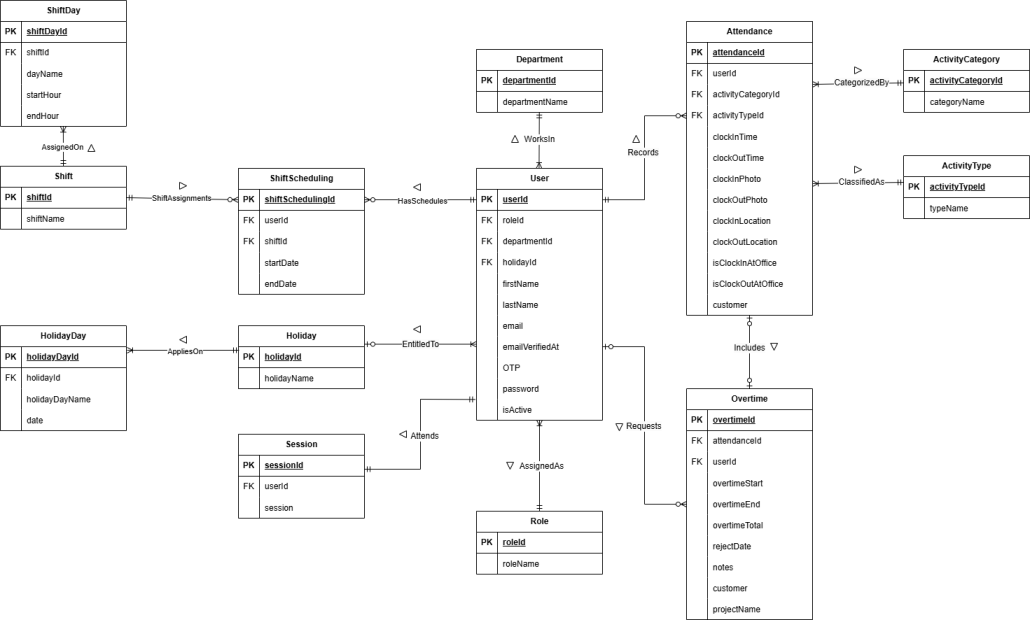
\includegraphics[width=17cm]{Gambar/bab2/logical-database-design.png}
	\caption{\textit{Logical Data Modeling}}
	\label{fig:logical-database-design}
\end{figure}


\begin{landscape}
\nextappendix
\section*{Lampiran \theappendixletter: \textit{Table Specification}
\label{sec:table-specification}}
\addcontentsline{toc}{section}{Lampiran \theappendixletter: \textit{Table Specification}}
\begin{longtable}{ |p{3cm}|p{3cm}|p{4cm}|p{3cm}|p{2cm}|p{2cm}|p{2cm}|}
\caption{\textit{Table Specification}}\label{tab:table-specification} 
\\
\hline
\textbf{\textit{Entity}}
&\textbf{\textit{Attributes}}
&\textbf{\textit{Description}}
&\textbf{\textit{Data Types}}
&\textbf{\textit{Nullvalue}}
&\textbf{\textit{Multivalue}}
&\textbf{\textit{Composite}}
\\ 
\hline

\multirow{9}{*}{\textit{User}}
&userId
&Primary key
&INT
&No
&No
&No
\\
\cline{2-7}
&roleId
&Foreign key \textit{entity} Role
&INT
&No
&No
&No
\\ 
\cline{2-7}
&departmentId
&Foreign key \textit{entity} Department
&INT
&No
&No
&No
\\ 
\cline{2-7}
&holidayId
&Foreign key \textit{entity} Holiday
&INT
&Yes
&No
&No
\\ 
\cline{2-7}
&emailVerifiedAt
&Waktu verifikasi \textit{email}
&Datetime
&yes
&No
&No
\\ 
\cline{2-7}
&firstName
&Nama depan user
&VARCHAR(50)
&No
&No
&No
\\ 
\cline{2-7}
&lastName
&Nama belakang user
&VARCHAR(50)
&No
&No
&No
\\ 
\cline{2-7}
&email
&Email user yang unik
&VARCHAR(50)
&No
&No
&No
\\ 
\cline{2-7}
&password
&Password user dalam bentuk hash.
&VARCHAR(50)
&No
&No
&No
\\ 
\hline

\multirow{2}{*}{}
&isActive
&Status apakah user aktif atau tidak.
&BOOLEAN
&No
&No
&No
\\ 
\cline{2-7}
&OTP
&6 digit kode OTP untuk verifikasi \textit{email}
&INT
&Yes
&No
&No
\\ 
\hline

\multirow{3}{*}{\textit{Session}}
&sessionId
&Primary key
&INT
&No
&No
&No
\\
\cline{2-7}
&userId
&Foreign key \textit{entity} User
&INT
&No
&No
&No
\\ 
\cline{2-7}
&session
&Pengenal unik yang mendefinisikan sesi pengguna saat login
&String
&No
&No
&No
\\ 
\hline

\multirow{4}{*}{\textit{Attendance}}
&attendanceId
&Primary key
&INT
&No
&No
&No
\\
\cline{2-7}
&userId
&Foreign key \textit{entity} User
&INT
&No
&No
&No
\\ 
\cline{2-7}
&activityTypeId
&Foreign key \textit{entity} ActivityType
&INT
&No
&No
&No
\\ 
\cline{2-7}
&activityCategoryId
&Foreign key \textit{entity} ActivityCategory
&INT
&No
&No
&No
\\ 
\hline

\multirow{8}{*}{}
&clockInTime
&Waktu user melakukan \textit{clock in}
&DATETIME
&No
&No
&No
\\ 
\cline{2-7}
&clockOutTime
&Waktu user melakukan \textit{clock out}
&DATETIME
&Yes
&No
&No
\\ 
\cline{2-7}
&clockInPhoto 
&\textit{Path} ke foto saat \textit{clock in}
&VARCHAR(255)
&No
&No
&No
\\ 
\cline{2-7}
&clockOutPhoto
&\textit{Path} ke foto saat \textit{clock out}
&VARCHAR(255)
&Yes
&No
&No
\\ 
\cline{2-7}
&clockInLocation
&Lokasi saat \textit{clock in}
&VARCHAR(255)
&No
&No
&No
\\ 
\cline{2-7}
&clockOutLocation
&Lokasi saat \textit{clock out}
&VARCHAR(255)
&Yes
&No
&No
\\ 
\cline{2-7}
&customer
&Nama customer saat presensi
&String
&Yes
&No
&No
\\ 
\cline{2-7}
&isClockInAtOffice
&Informasi terkait presensi masuk dilakukan diluar atau didalam radius kantor
&Boolean
&No
&No
&No
\\ 
\hline

\multirow{1}{*}{}
&isClockOutAtOffice
&Informasi terkait presensi keluar dilakukan diluar atau didalam radius kantor
&Boolean
&No
&No
&No
\\ 
\hline

\multirow{2}{*}{\textit{Department}}
&departmentId
&Primary key
&INT
&No
&No
&No
\\
\cline{2-7}
&departmentName
&Nama departemen atau divisi dari user
&VARCHAR(50)
&No
&No
&No
\\ 
\hline

\multirow{2}{*}{\textit{Role}}
&roleId
&Primary key
&INT
&No
&No
&No
\\
\cline{2-7}
&roleName
&Nama role atau jabatan dari user
&VARCHAR(50)
&No
&No
&No
\\ 
\hline

\multirow{2}{*}{\textit{Shift}}
&shiftId
&Primary key
&INT
&No
&No
&No
\\
\cline{2-7}
&shiftName
&Nama shift kerja
&VARCHAR(50)
&No
&No
&No
\\ 
\hline

\multirow{3}{*}{\textit{ShiftDay}}
&shiftDayId
&Primary key
&INT
&No
&No
&No
\\
\cline{2-7}
&shiftId
&Foreign key \textit{entity} Shift
&INT
&No
&No
&No
\\
\cline{2-7}
&dayName
&Nama hari dari setiap \textit{shift} kerja
&VARCHAR(20)
&No
&No
&No
\\
\hline

\multirow{2}{*}{}
&startHour
&Waktu mulai \textit{shift} kerja
&TIME
&No
&No
&No
\\
\cline{2-7}
&endHour
&Waktu selesai \textit{shift} kerja
&TIME
&No
&No
&No
\\ 
\hline

\multirow{2}{*}{\textit{Holiday}}
&Holiday
&Primary key
&INT
&No
&No
&No
\\
\cline{2-7}
&holidayName
&Nama jenis libur
&VARCHAR(50)
&No
&No
&No
\\ 
\hline

\multirow{4}{*}{\textit{HolidayDay}}
&holidayDayId
&Primary key
&INT
&No
&No
&No
\\
\cline{2-7}
&holidayId
&Foreign key \textit{entity} Holiday
&INT
&No
&No
&No
\\
\cline{2-7}
&date
&Tanggal hari libur perusahaan
&DATE
&No
&No
&No
\\
\cline{2-7}
&holidayName
&Nama hari libur perusahaan
&VARCHAR(50)
&No
&No
&No
\\ 
\hline

\multirow{3}{*}{\textit{Overtime}}
&overtimeId
&Primary key
&INT
&No
&No
&No
\\
\cline{2-7}
&attendanceId
&Foreign key \textit{entity} Attendance
&INT
&Yes
&No
&No
\\ 
\cline{2-7}
&userId
&Foreign key \textit{entity} User
&INT
&Yes
&No
&No
\\ 
\hline

\multirow{7}{*}{}
&overtimeStart 
&Waktu mulai lembur
&DATETIME
&No
&No
&No
\\ 
\cline{2-7}
&overtimeEnd 
&Waktu berakhir lembur
&DATETIME
&No
&No
&No
\\ 
\cline{2-7}
&overtimeTotal
&Jumlah lembur dalam menit
&FLOAT
&No
&No
&No
\\ 
\cline{2-7}
&notes
&Catatan tambahan mengenai lembur
&VARCHAR(255)
&Yes
&No
&No
\\ 
\cline{2-7}
&rejectDate 
&Tanggal penolakan lembur
&DATETIME
&Yes
&No
&No
\\ 

\cline{2-7}
&customer 
&Nama pelanggan terkait lembur
&VARCHAR(100)
&Yes
&No
&No
\\ 
\cline{2-7}
&projectName 
&Nama \textit{project} yang dikerjakan saat lembur
&VARCHAR(100)
&Yes
&No
&No
\\ 
\hline

\multirow{2}{*}{\textit{ActivityType}}
&activityTypeId
&Primary key
&INT
&No
&No
&No
\\
\cline{2-7}
&activityTypeName
&Nama tipe aktivitas saat presensi 
&VARCHAR(50)
&No
&No
&No
\\ 
\hline

\multirow{2}{*}{\textit{ActivityCategory}}
&activityCategoryId
&Primary key
&INT
&No
&No
&No
\\
\cline{2-7}
&activityCategoryName
&Nama kategori aktivitas saat presensi
&VARCHAR(50)
&No
&No
&No
\\ 
\hline

\multirow{5}{*}{\textit{ShiftScheduling}}
&shiftSchedulingId
&Primary key
&INT
&No
&No
&No
\\
\cline{2-7}
&userId
&Foreign key \textit{entity} User
&INT
&No
&No
&No
\\
\cline{2-7}
&shiftId
&Foreign key \textit{entity} Shift
&INT
&No
&No
&No
\\
\cline{2-7}
&startDate
&Tanggal mulai jadwal shift
&DATETIME
&No
&No
&No
\\
\cline{2-7}
&endDate
&Tanggal selesai jadwal shift
&DATETIME
&No
&No
&No
\\ 
\hline



\end{longtable}
\pagebreak
\end{landscape}

\nextappendix
\section*{Lampiran \theappendixletter: \textit{Mockup} Aplikasi Presensi \textit{Online}
\label{sec:mockup-aplikasi-presensi-online}}
\addcontentsline{toc}{section}{Lampiran \theappendixletter: \textit{Mockup} Aplikasi Presensi \textit{Online}}
\begin{figure}[H]
    \centering
    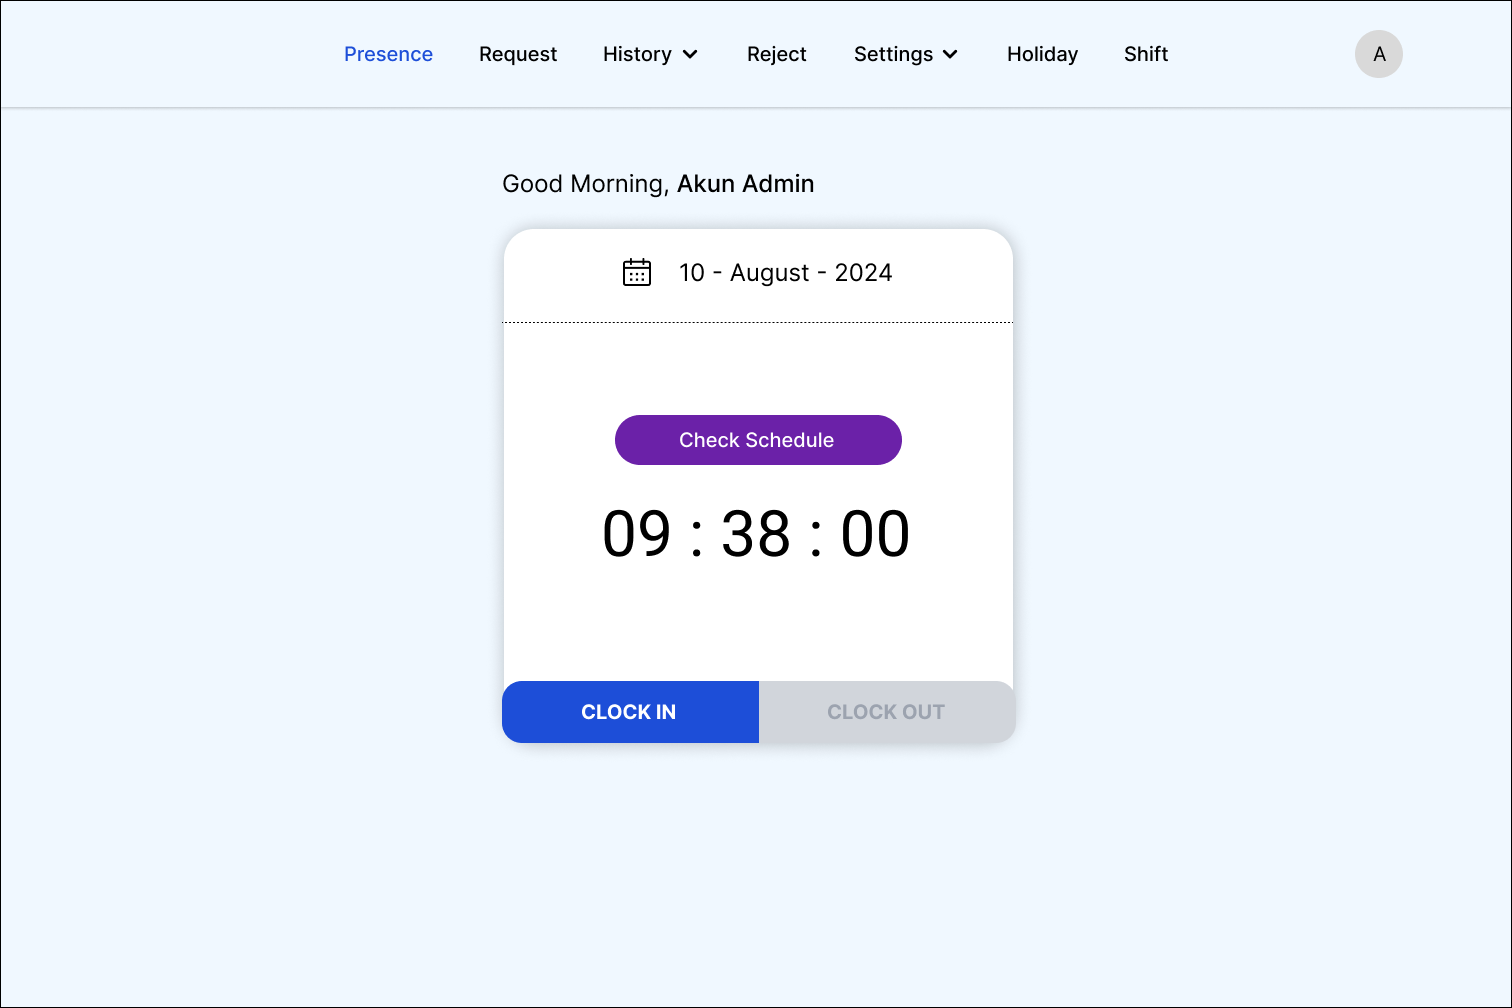
\includegraphics[width=13cm]{Gambar/bab2/mockups/menu-utama.png}
    \caption{\textit{Mockup} Menu Utama}
    \label{fig:mockup-menu-utama}
\end{figure}
\FloatBarrier


\begin{figure}[H]
	\centering
	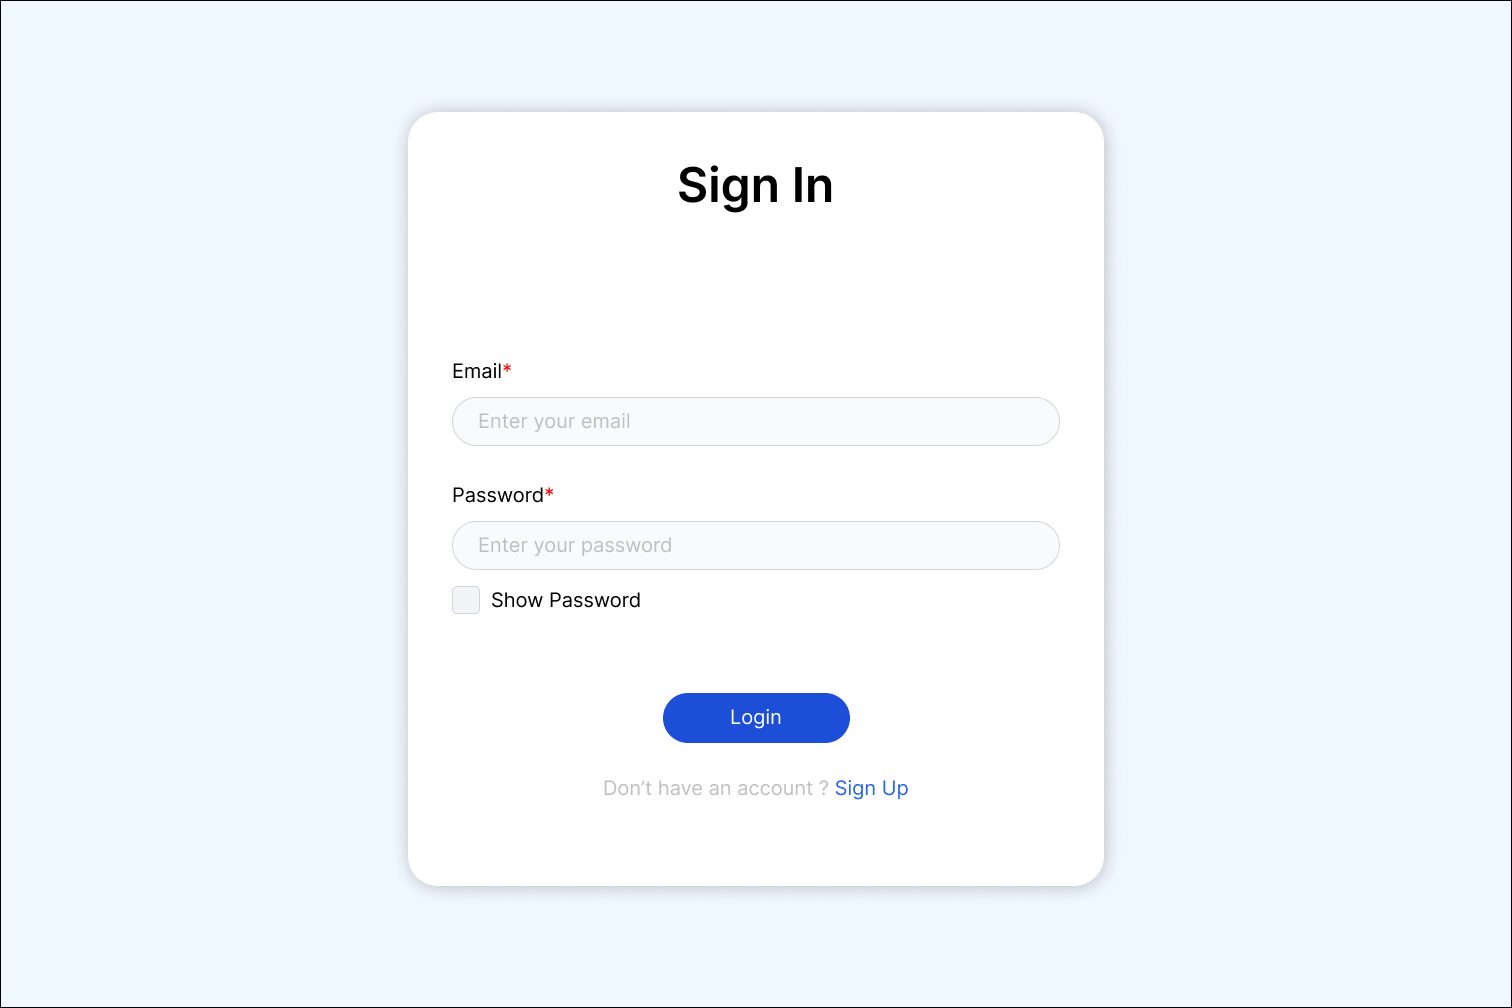
\includegraphics[width=13cm]{Gambar/bab2/mockups/menu-login.png}
	\caption{\textit{Mockup} Menu \textit{Login}}
	\label{fig:mockup-menu-login}
\end{figure}
\FloatBarrier

\begin{figure}[H]
	\centering
	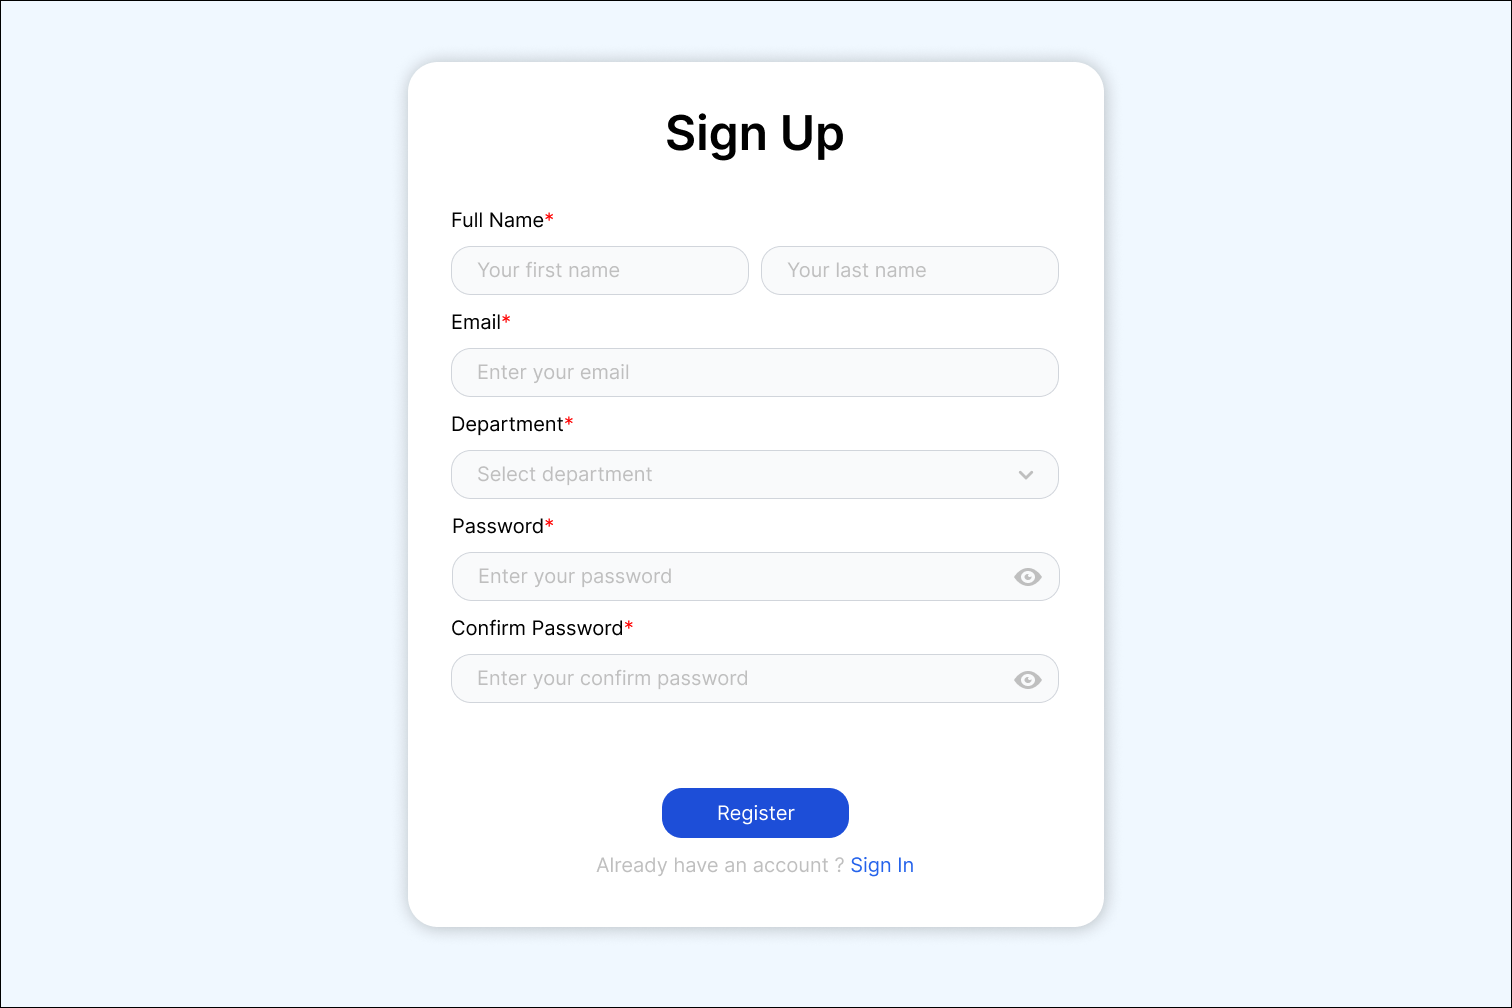
\includegraphics[width=13cm]{Gambar/bab2/mockups/menu-registrasi-akun.png}
	\caption{\textit{Mockup} Menu Registrasi Akun}
	\label{fig:mockup-menu-registrasi-akun}
\end{figure}
\FloatBarrier

\begin{figure}[H]
	\centering
	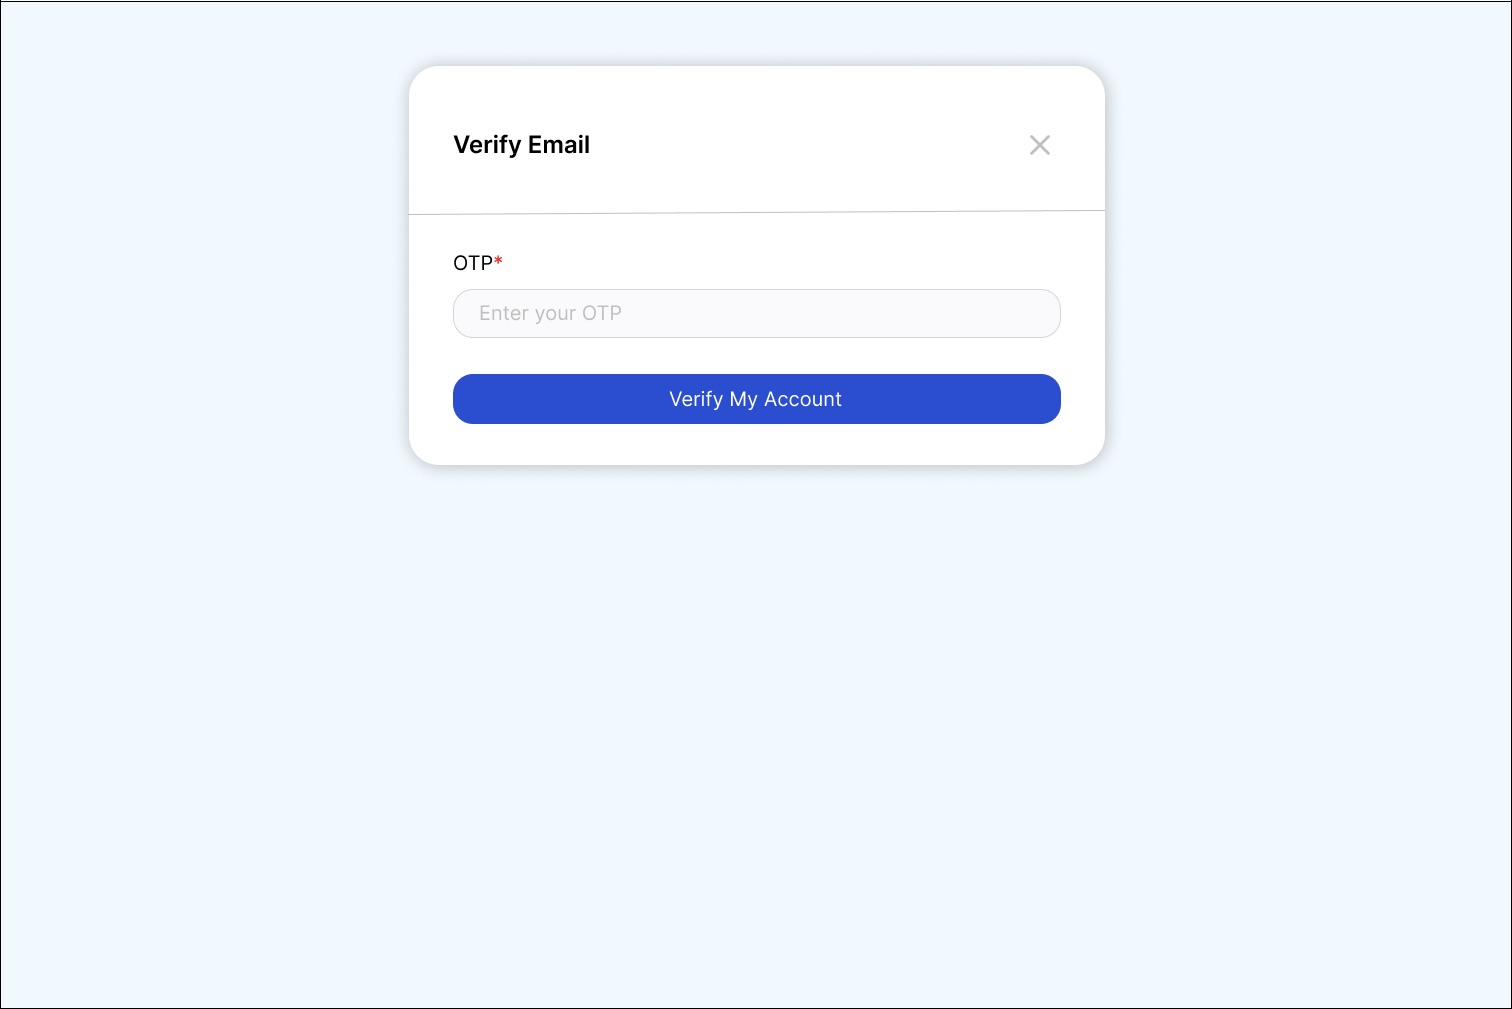
\includegraphics[width=13cm]{Gambar/bab2/mockups/menu-verifikasi-email.png}
	\caption{\textit{Mockup} Menu Verifikasi \textit{Email}}
	\label{fig:mockup-menu-verifikasi-email}
\end{figure}
\FloatBarrier

\begin{figure}[H]
	\centering
	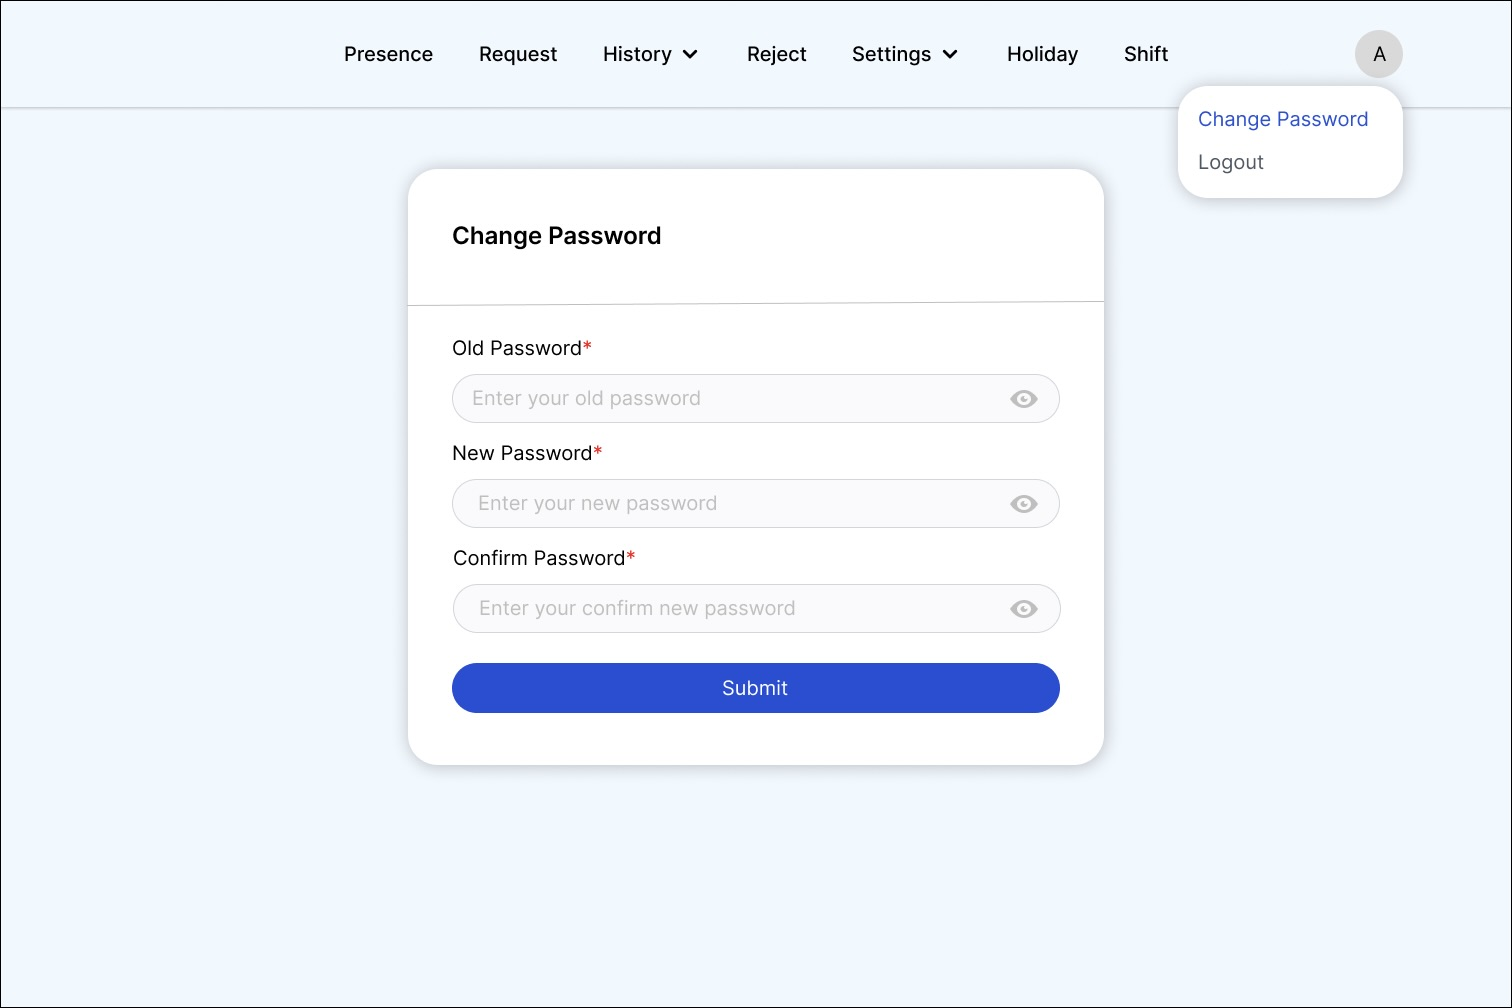
\includegraphics[width=13cm]{Gambar/bab2/mockups/menu-ganti-password.png}
	\caption{\textit{Mockup} Menu Ganti Password}
	\label{fig:mockup-menu-ganti-password}
\end{figure}
\FloatBarrier

\begin{figure}[H]
	\centering
	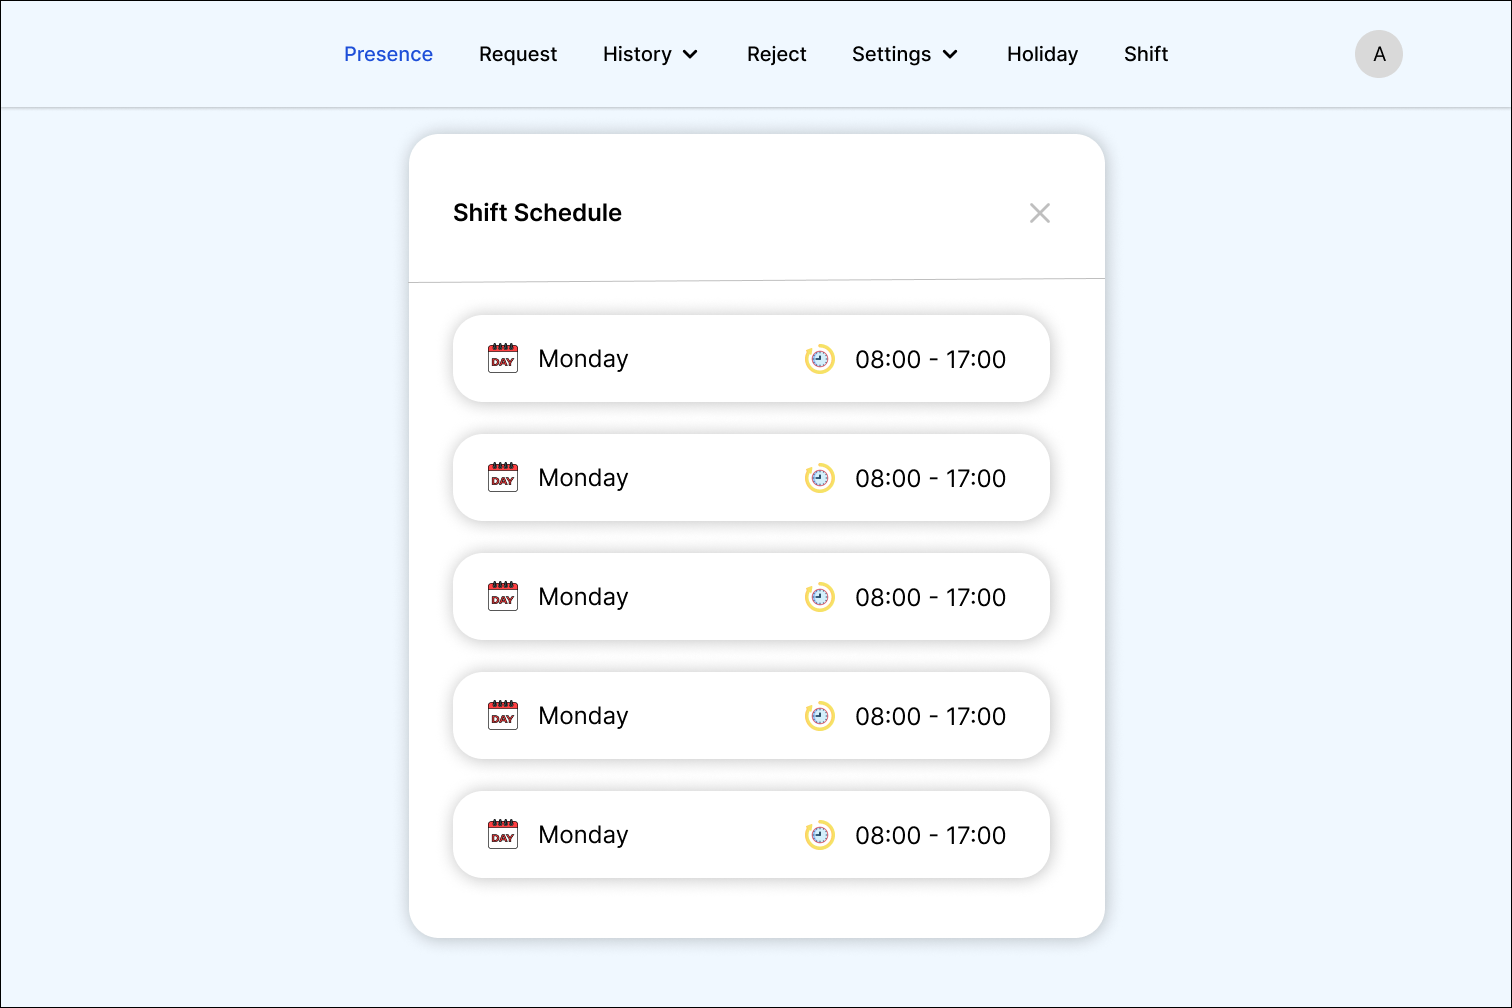
\includegraphics[width=13cm]{Gambar/bab2/mockups/menu-jadwal-shift.png}
	\caption{\textit{Mockup} Menu Jadwal \textit{Shift}}
	\label{fig:mockup-menu-jadwal-shift}
\end{figure}
\FloatBarrier

\begin{figure}[H]
	\centering
	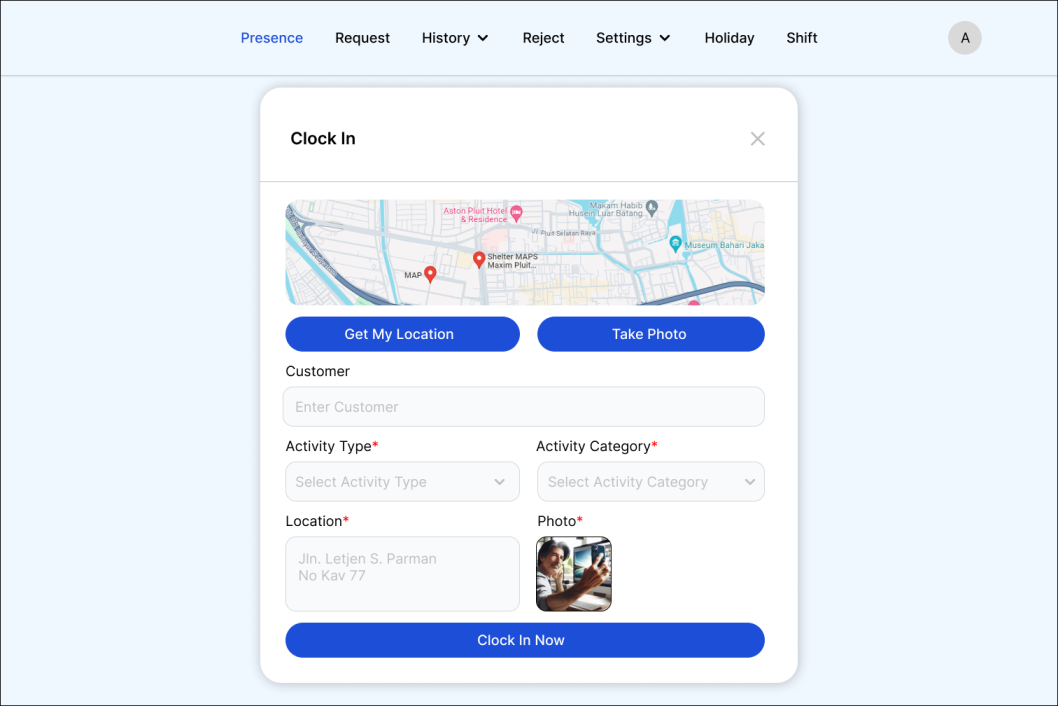
\includegraphics[width=13cm]{Gambar/bab2/mockups/menu-clock-in.png}
	\caption{\textit{Mockup} Menu \textit{Clock In}}
	\label{fig:mockup-menu-clock-in}
\end{figure}
\FloatBarrier

\begin{figure}[H]
	\centering
	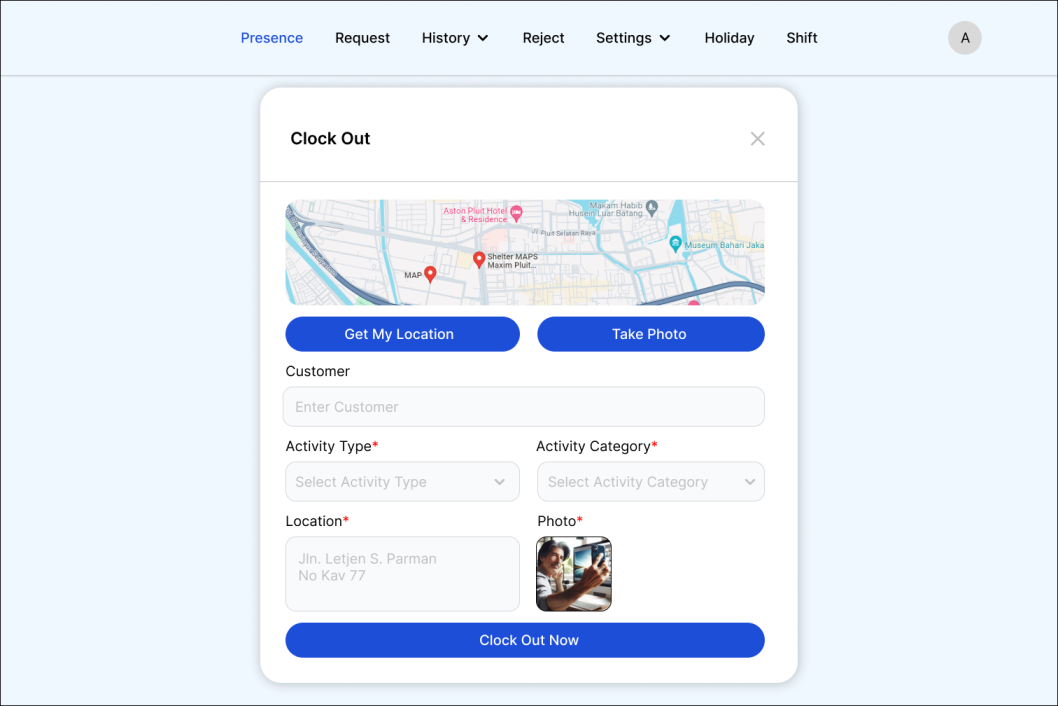
\includegraphics[width=13cm]{Gambar/bab2/mockups/menu-clock-out.png}
	\caption{\textit{Mockup} Menu \textit{Clock Out}}
	\label{fig:mockup-menu-clock-out}
\end{figure}
\FloatBarrier

\begin{figure}[H]
	\centering
	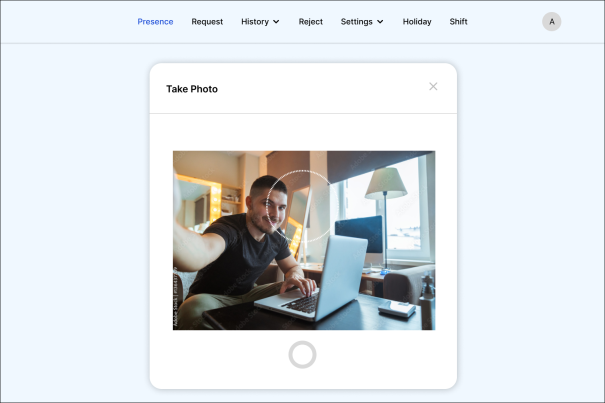
\includegraphics[width=13cm]{Gambar/bab2/mockups/menu-kamera.png}
	\caption{\textit{Mockup} Menu Kamera}
	\label{fig:mockup-menu-kamera}
\end{figure}
\FloatBarrier

\begin{figure}[H]
	\centering
	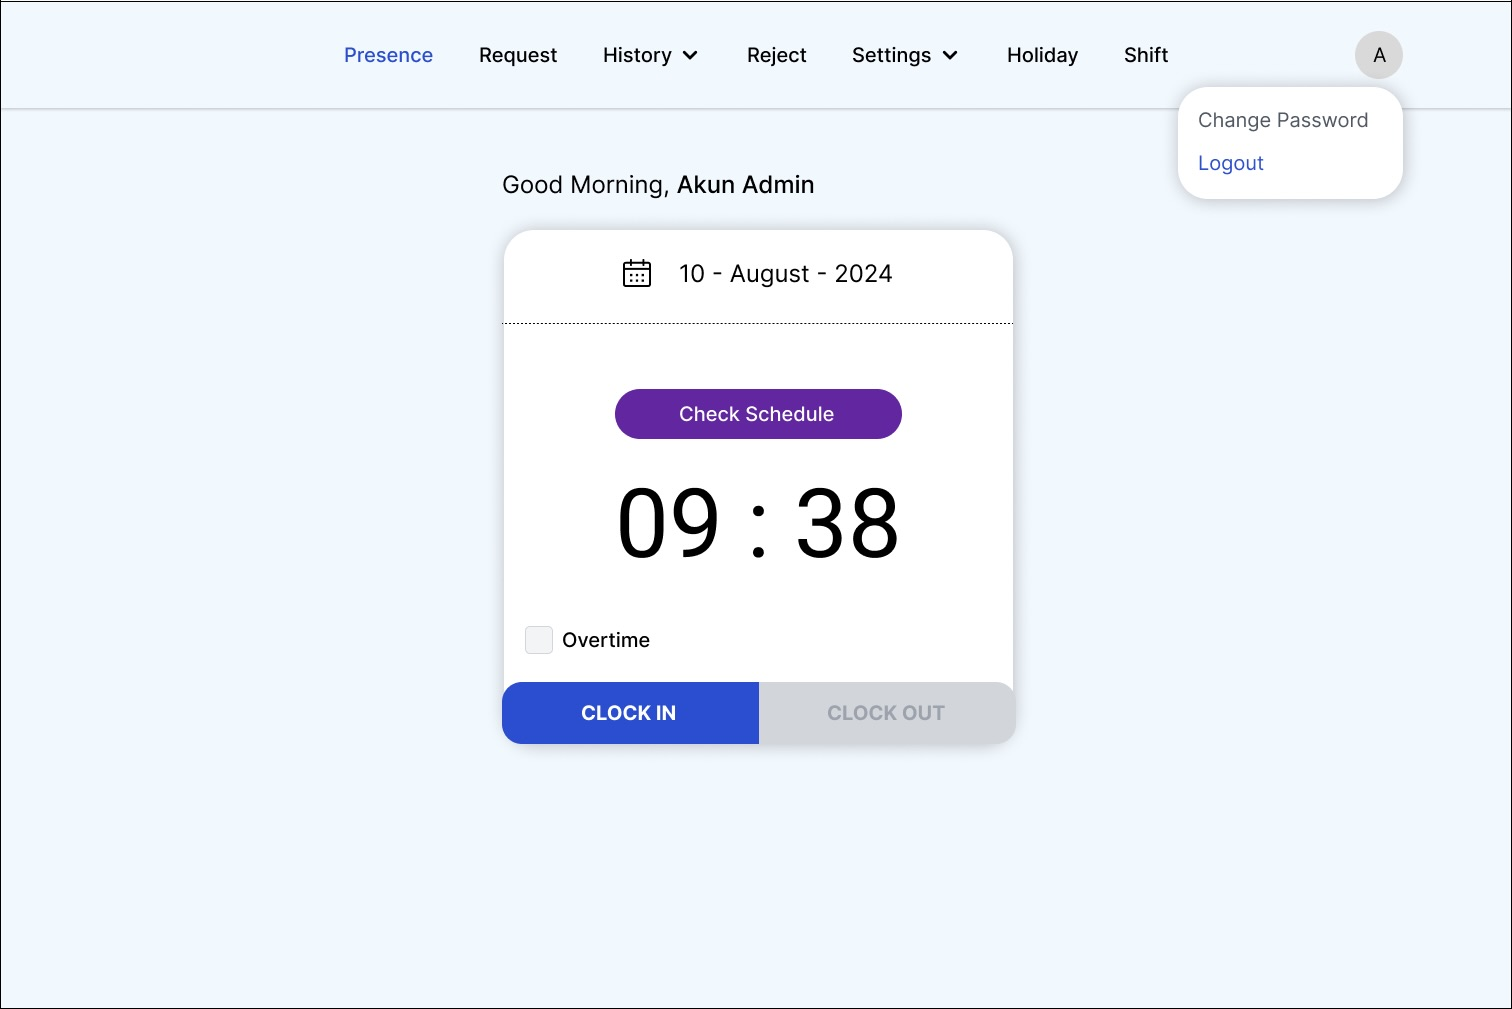
\includegraphics[width=13cm]{Gambar/bab2/mockups/menu-profil.png}
	\caption{\textit{Mockup} Menu Profil}
	\label{fig:mockup-menu-profil}
\end{figure}
\FloatBarrier

\begin{figure}[H]
	\centering
	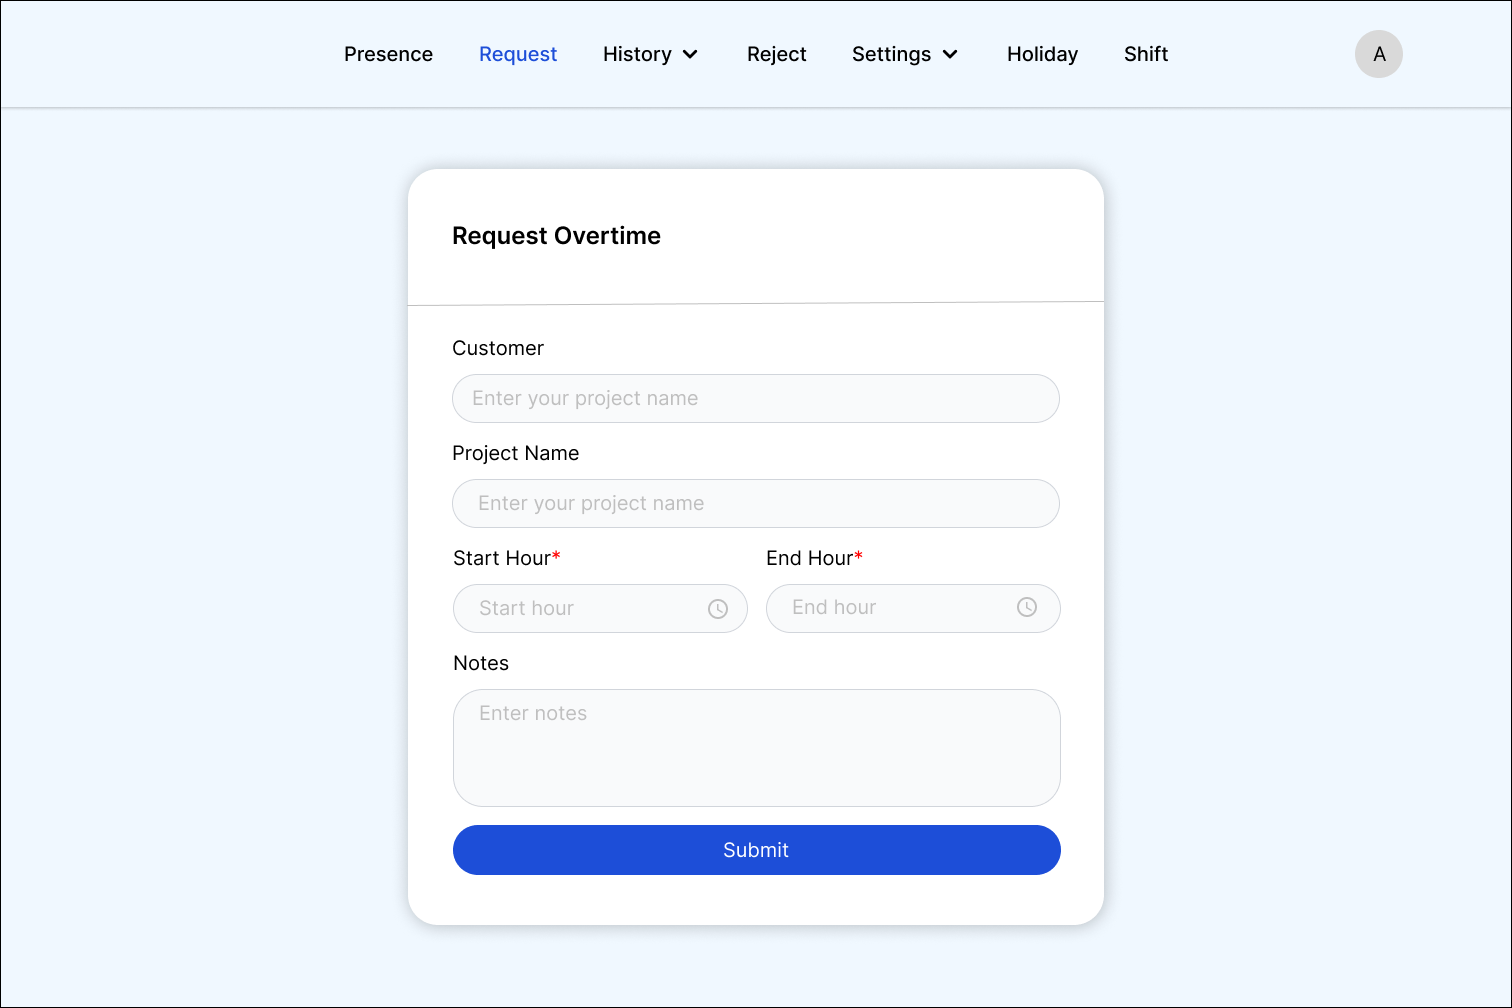
\includegraphics[width=13cm]{Gambar/bab2/mockups/menu-pengajuan-lembur.png}
	\caption{\textit{Mockup} Menu Pengajuan Lembur}
	\label{fig:mockup-menu-pengajuan-lembur}
\end{figure}
\FloatBarrier

\begin{figure}[H]
	\centering
	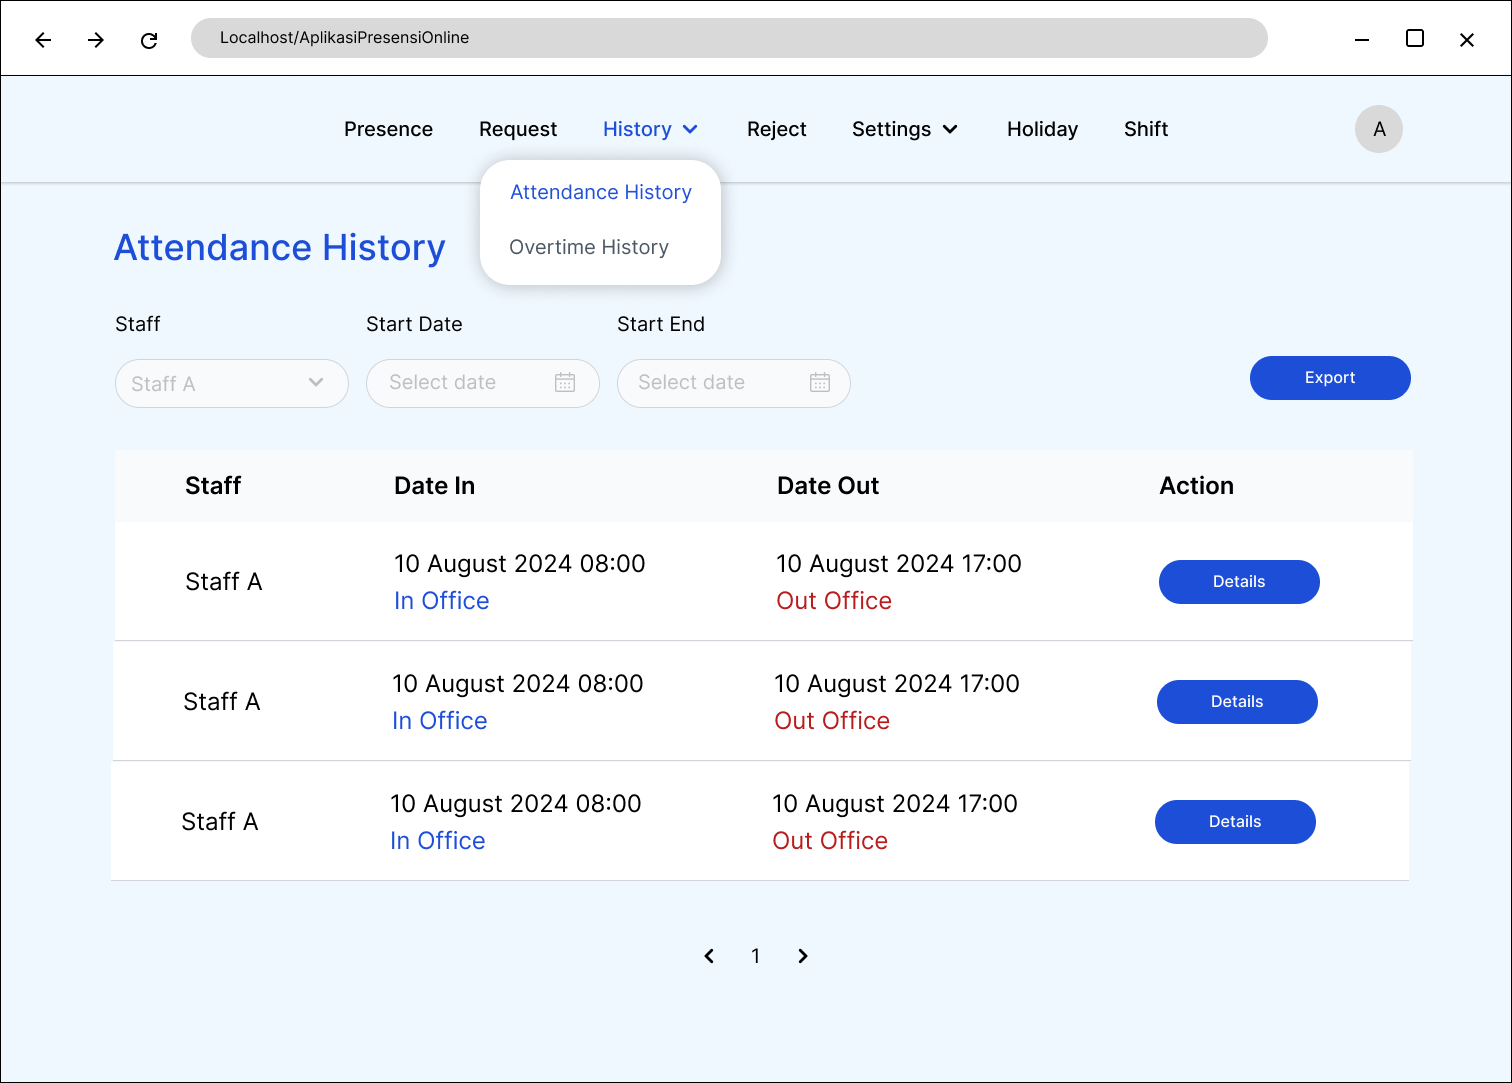
\includegraphics[width=13cm]{Gambar/bab2/mockups/menu-riwayat-presensi.png}
	\caption{\textit{Mockup} Menu Riwayat Presensi}
	\label{fig:mockup-menu-riwayat-presensi}
\end{figure}
\FloatBarrier

\begin{figure}[H]
	\centering
	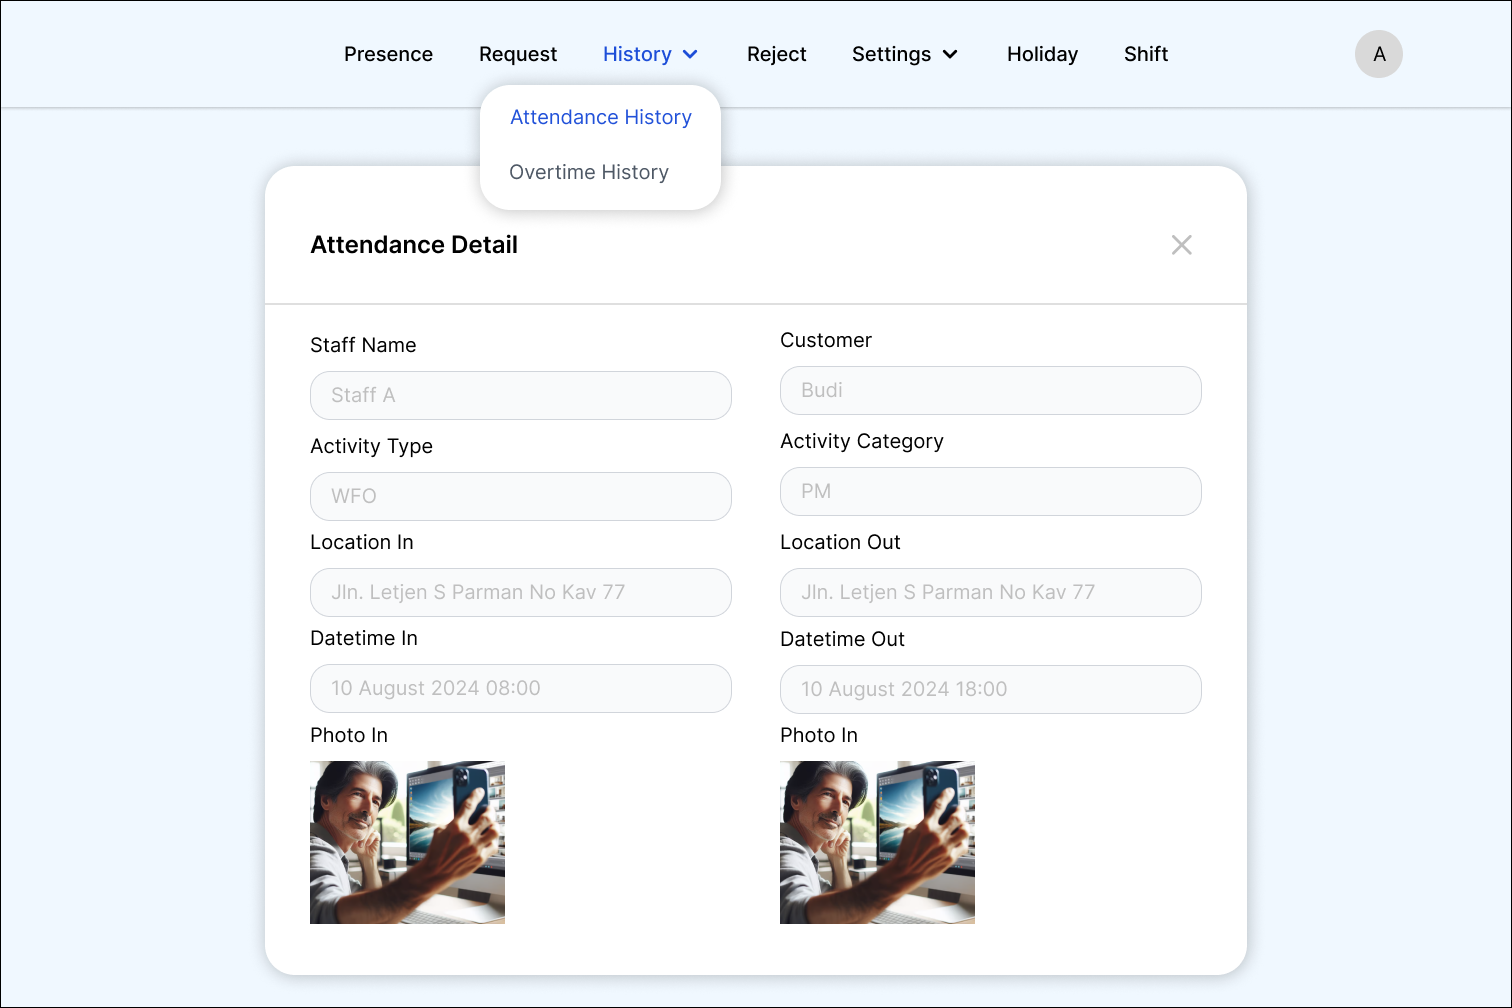
\includegraphics[width=13cm]{Gambar/bab2/mockups/menu-detail-presensi.png}
	\caption{\textit{Mockup} Menu Detail Presensi}
	\label{fig:mockup-menu-detail-presensi}
\end{figure}
\FloatBarrier

\begin{figure}[H]
	\centering
	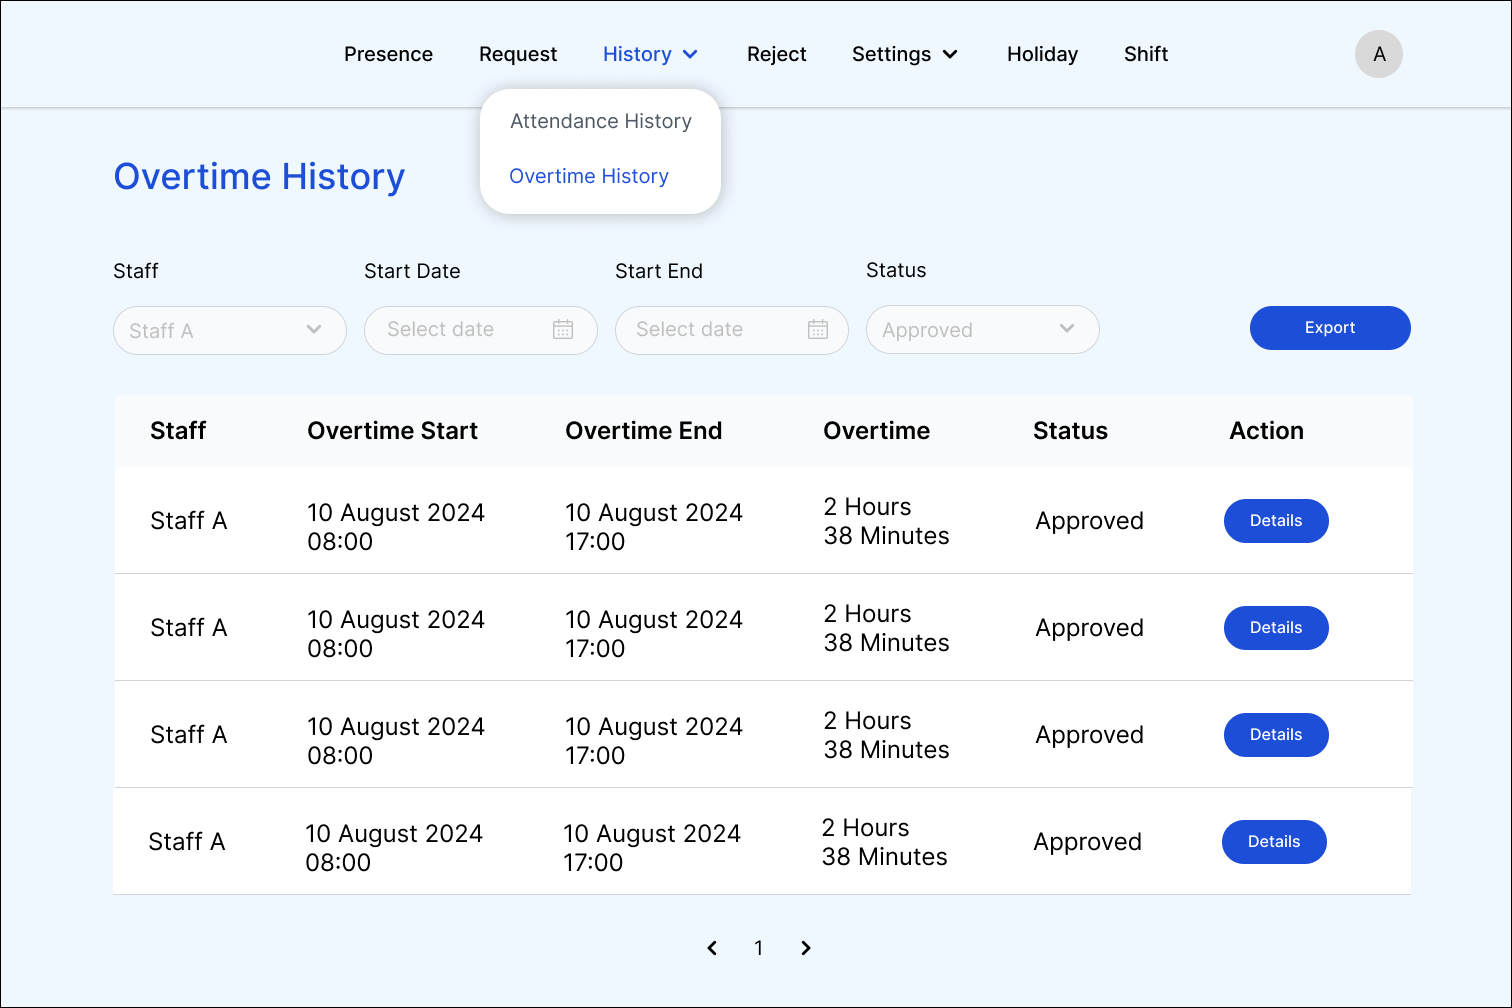
\includegraphics[width=13cm]{Gambar/bab2/mockups/menu-riwayat-lembur.png}
	\caption{\textit{Mockup} Menu Riwayat Lembur}
	\label{fig:mockup-menu-riwayat-lembur}
\end{figure}
\FloatBarrier

\begin{figure}[H]
	\centering
	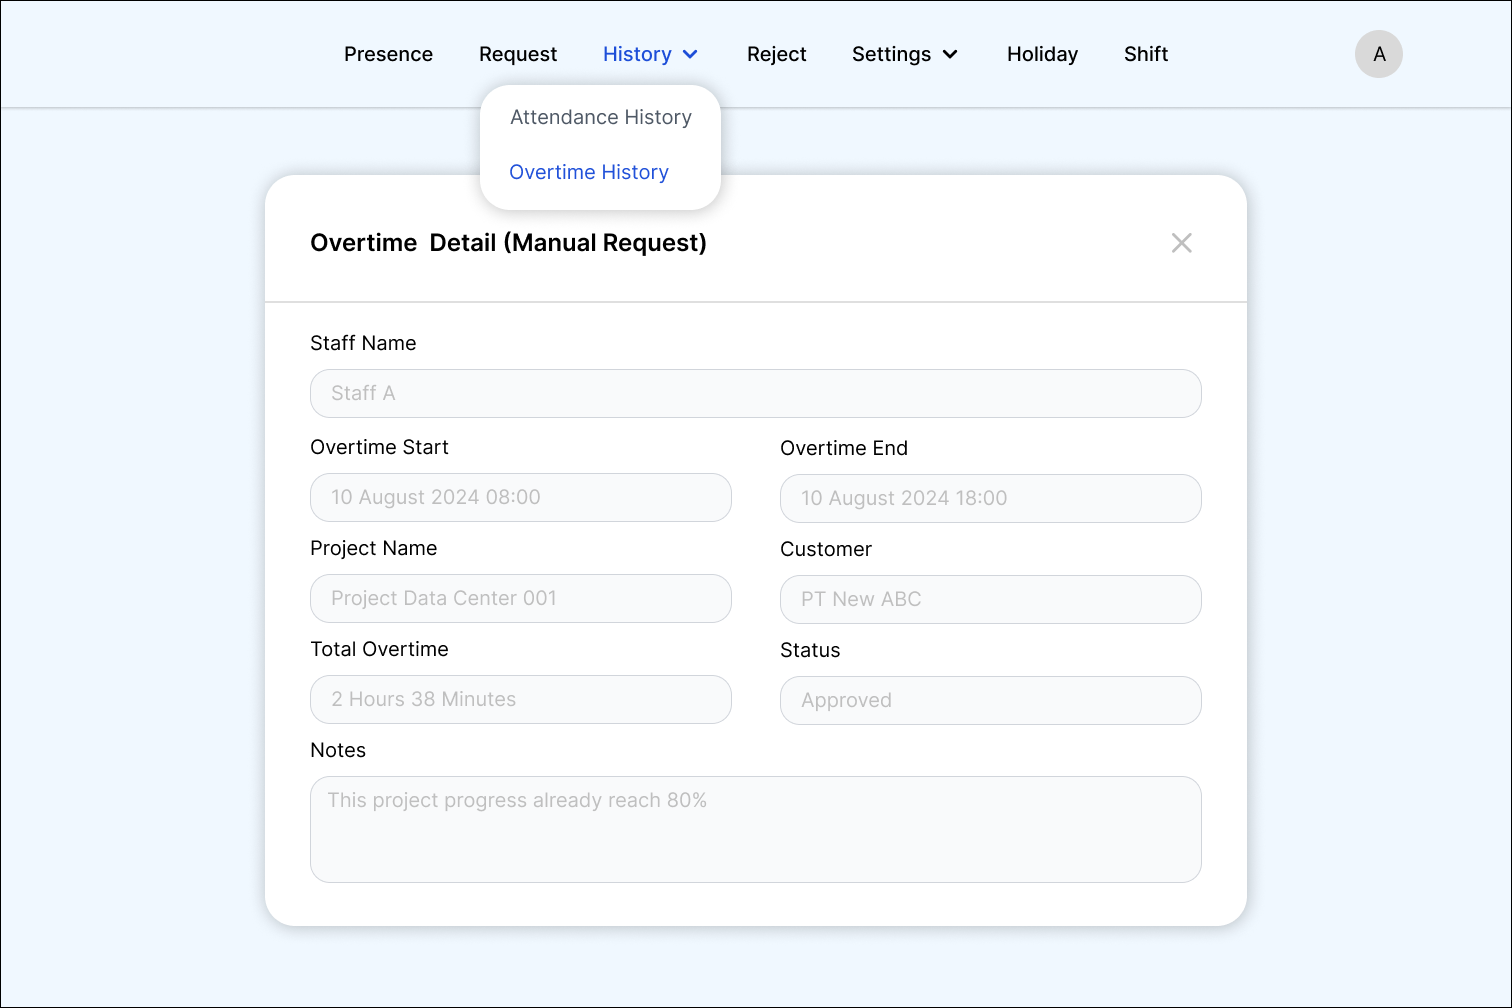
\includegraphics[width=13cm]{Gambar/bab2/mockups/menu-detail-lembur.png}
	\caption{\textit{Mockup} Menu Detail Lembur}
	\label{fig:mockup-menu-detail-lembur}
\end{figure}
\FloatBarrier

\begin{figure}[H]
	\centering
	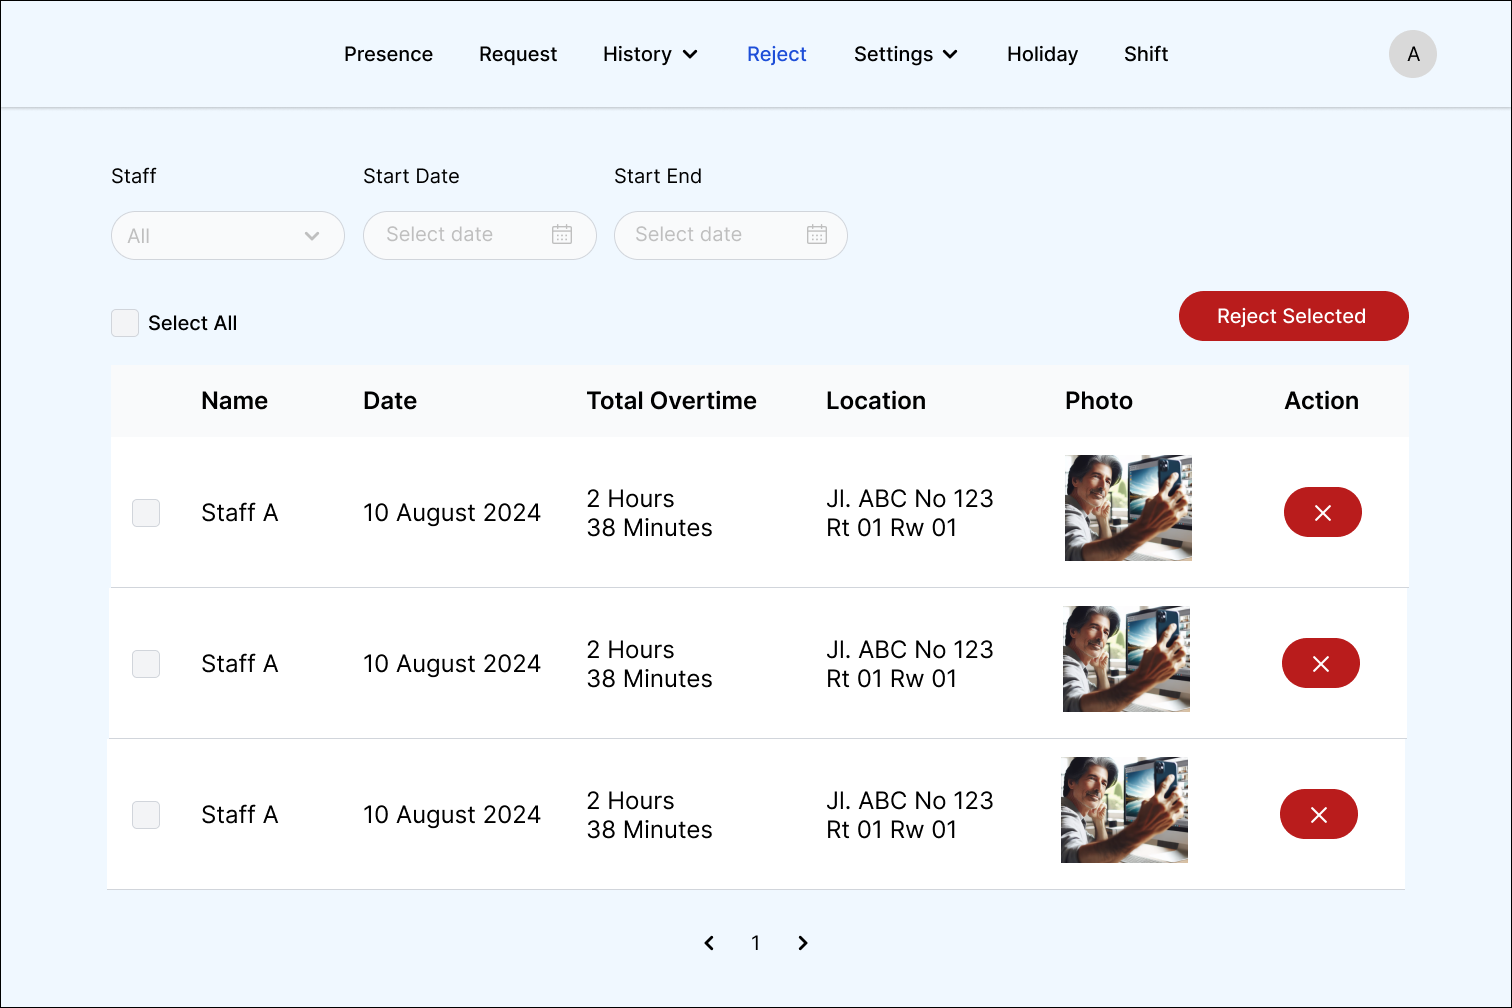
\includegraphics[width=13cm]{Gambar/bab2/mockups/menu-reject-lembur.png}
	\caption{\textit{Mockup} Menu \textit{Reject} Lembur}
	\label{fig:mockup-menu-reject-lembur}
\end{figure}
\FloatBarrier

\begin{figure}[H]
	\centering
	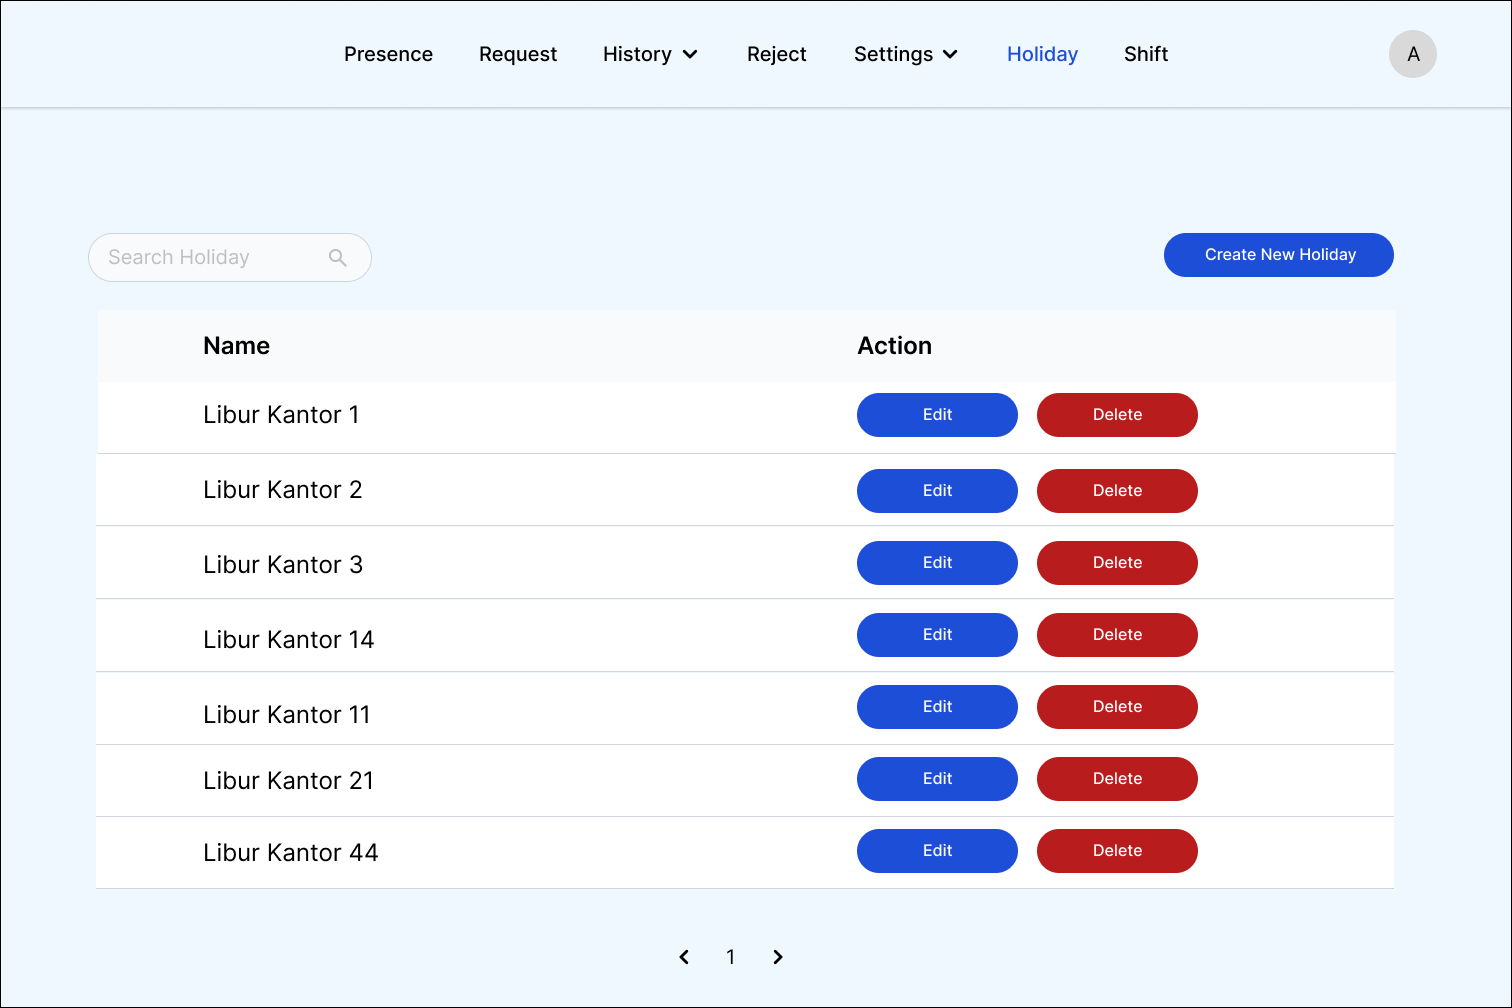
\includegraphics[width=13cm]{Gambar/bab2/mockups/menu-libur.png}
	\caption{\textit{Mockup} Menu Libur}
	\label{fig:mockup-menu-libur}
\end{figure}
\FloatBarrier

\begin{figure}[H]
	\centering
	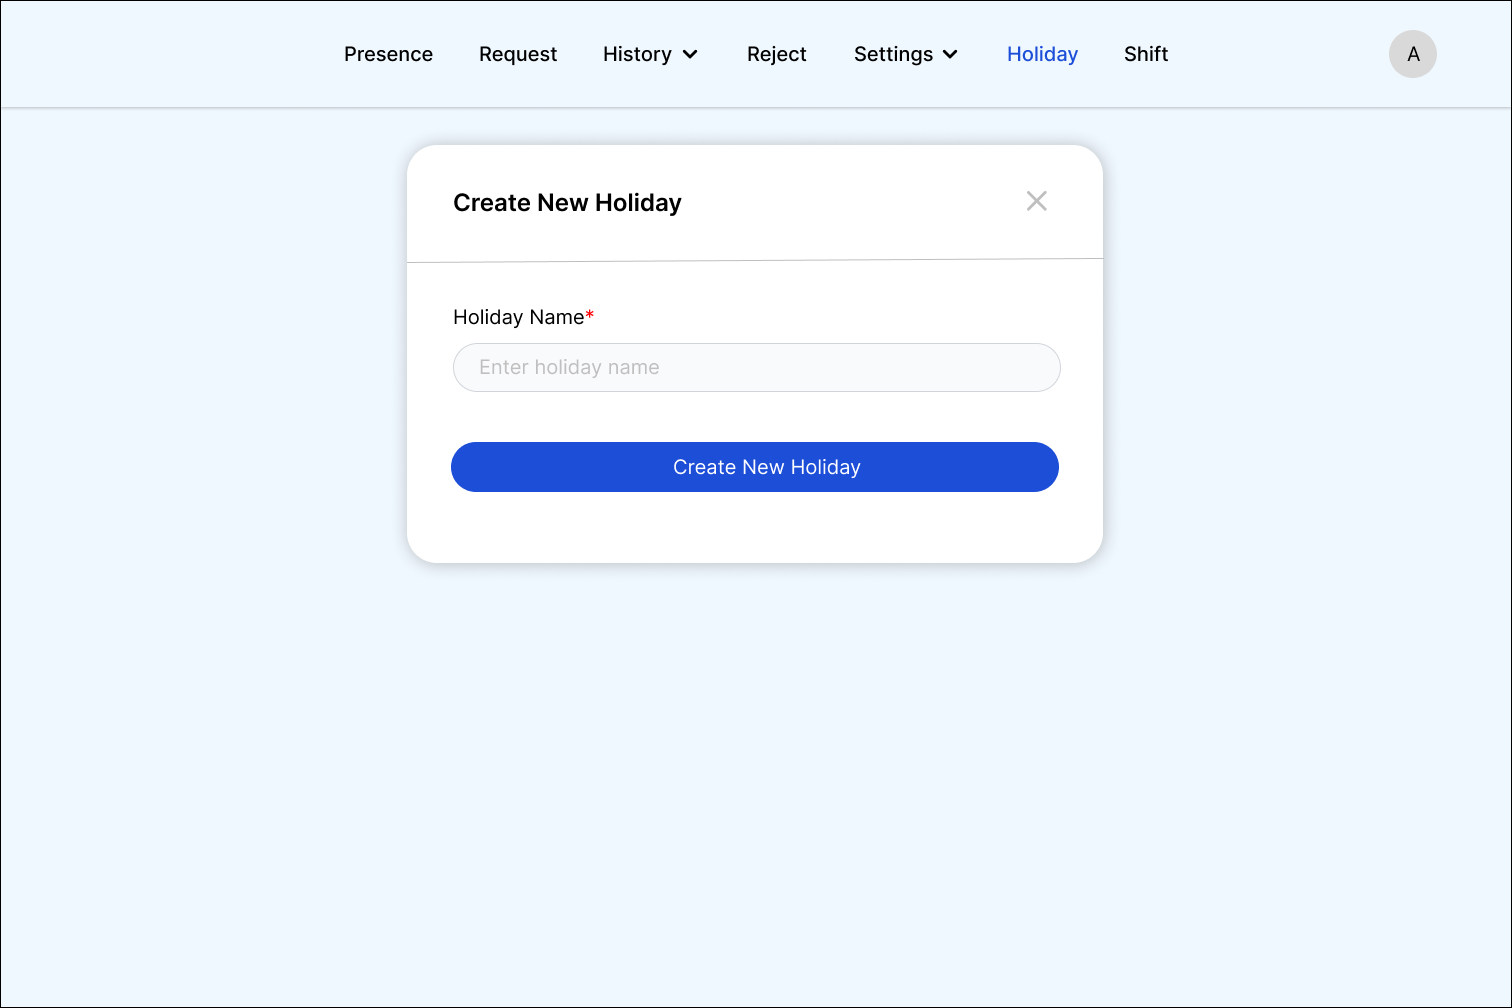
\includegraphics[width=13cm]{Gambar/bab2/mockups/menu-tambah-libur.png}
	\caption{\textit{Mockup} Menu Tambah Libur}
	\label{fig:mockup-menu-tambah-libur}
\end{figure}
\FloatBarrier

\begin{figure}[H]
	\centering
	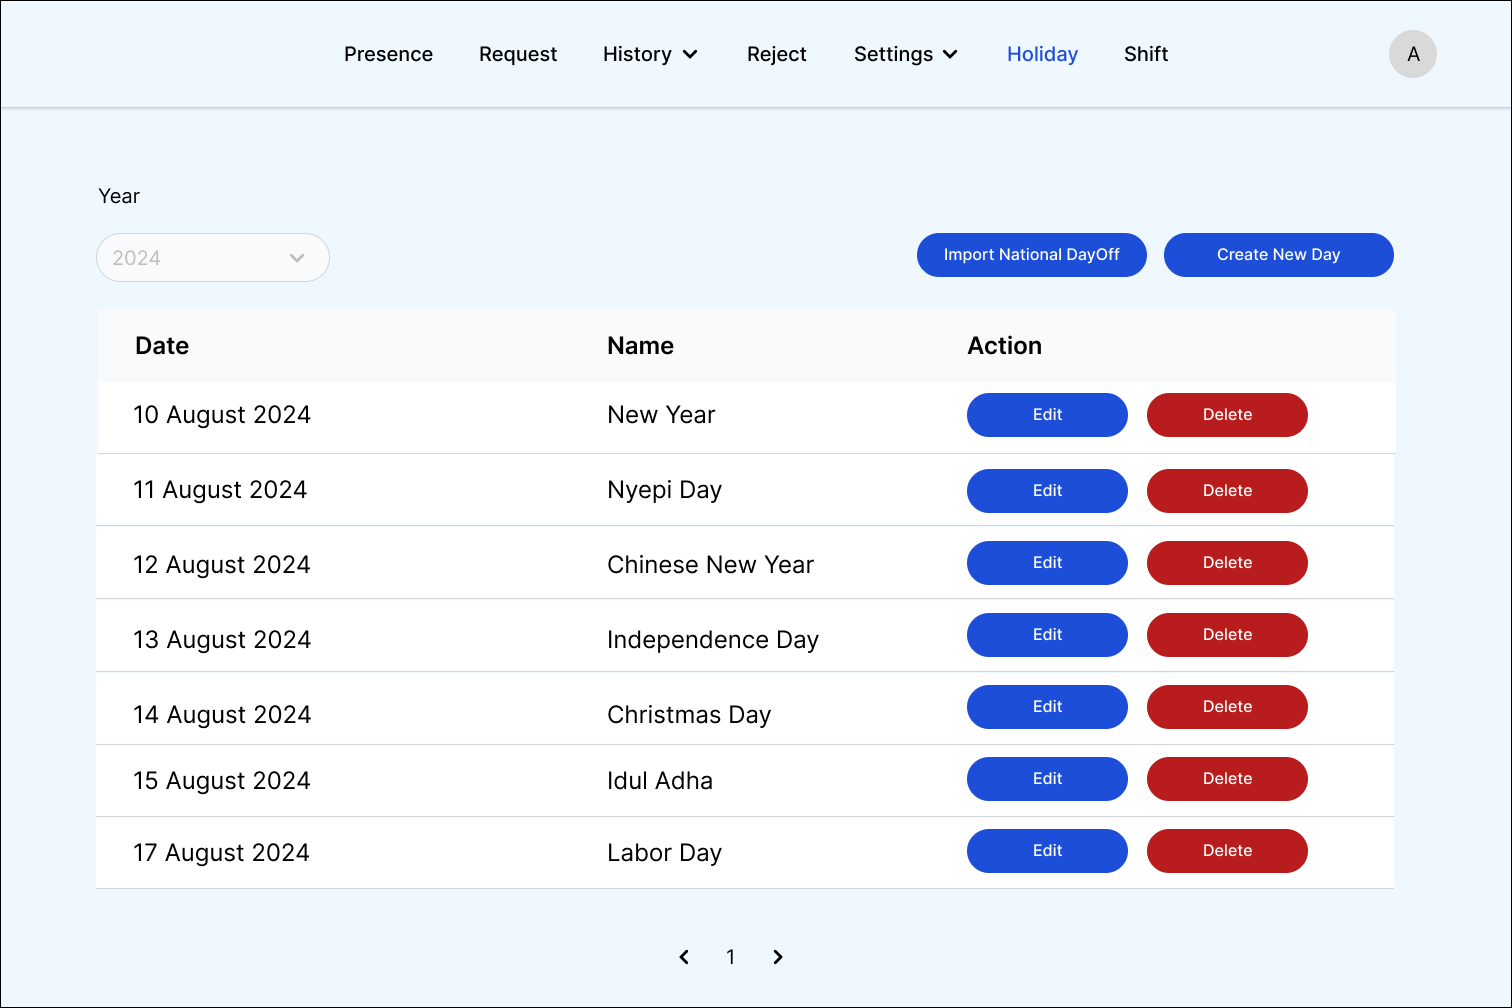
\includegraphics[width=13cm]{Gambar/bab2/mockups/menu-hari-libur.png}
	\caption{\textit{Mockup} Menu Hari Libur}
	\label{fig:mockup-menu-hari-libur}
\end{figure}
\FloatBarrier

\begin{figure}[H]
	\centering
	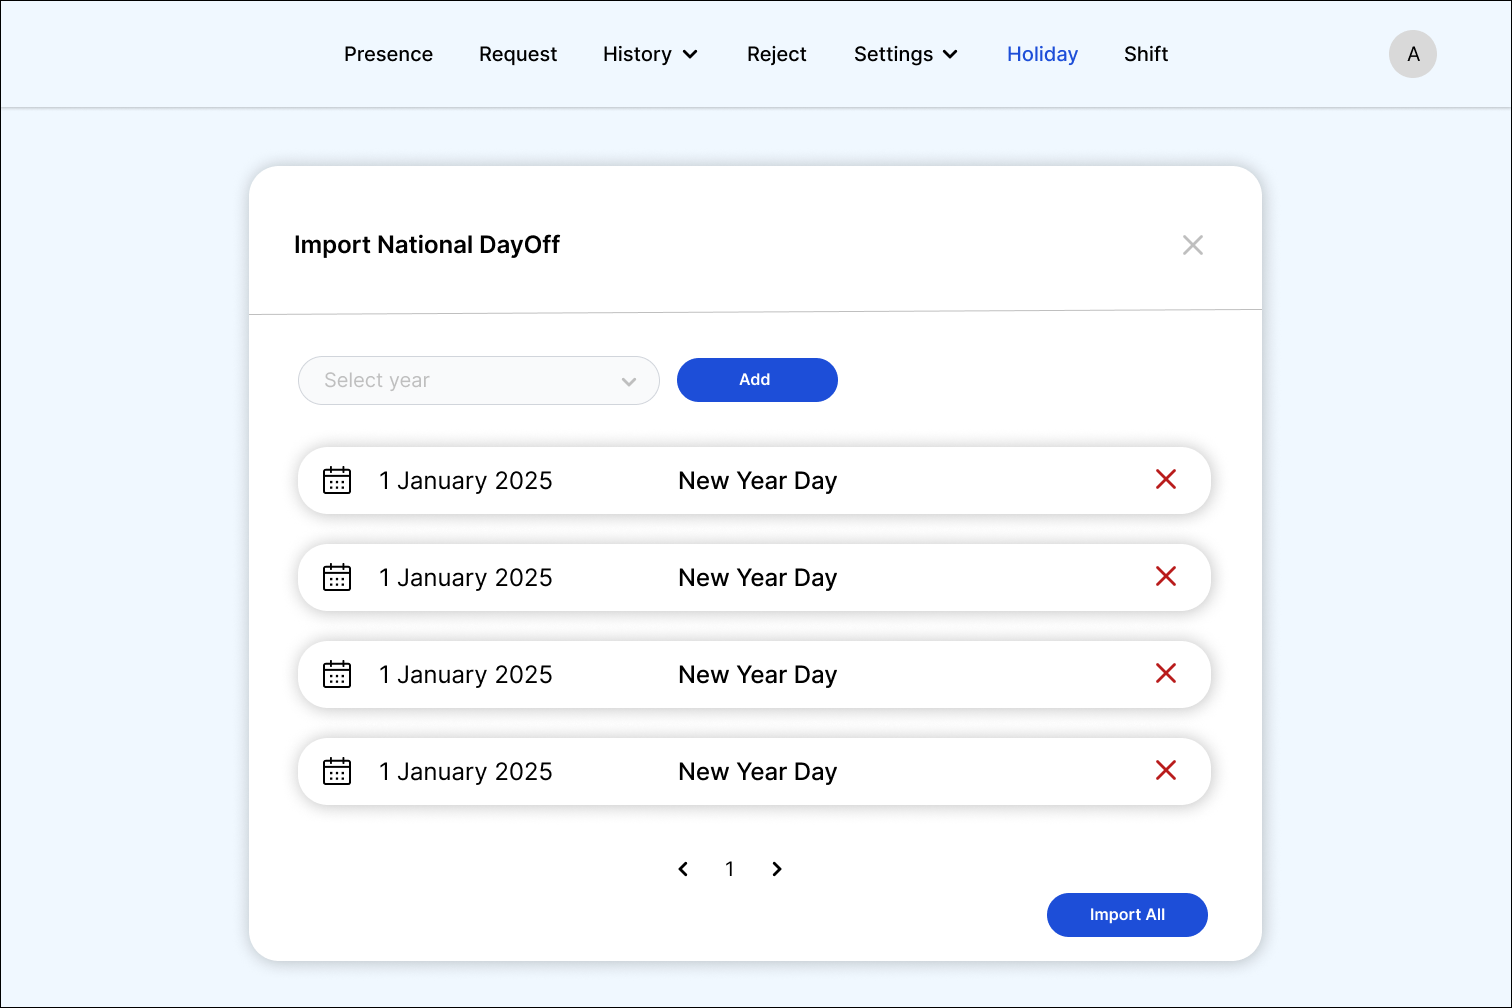
\includegraphics[width=13cm]{Gambar/bab2/mockups/menu-import-libur.png}
	\caption{\textit{Mockup} Menu \textit{Import} Libur}
	\label{fig:mockup-menu-import-libur}
\end{figure}
\FloatBarrier

\begin{figure}[H]
	\centering
	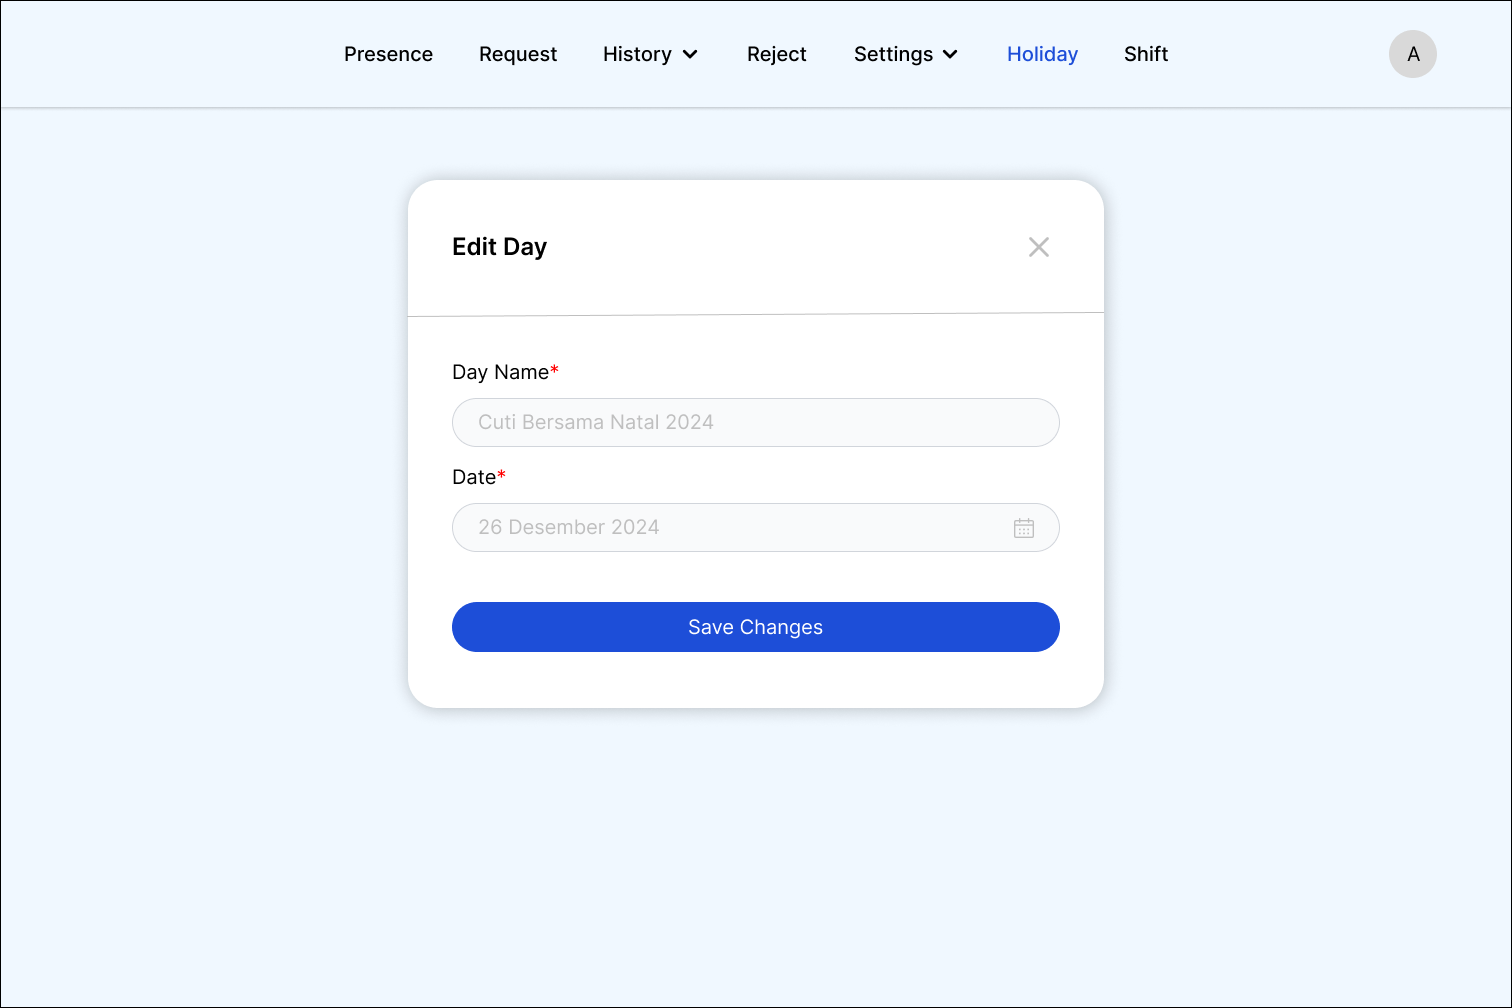
\includegraphics[width=13cm]{Gambar/bab2/mockups/menu-edit-hari-libur.png}
	\caption{\textit{Mockup} Menu \textit{Edit} Hari Libur}
	\label{fig:mockup-menu-edit-hari-libur}
\end{figure}
\FloatBarrier

\begin{figure}[H]
	\centering
	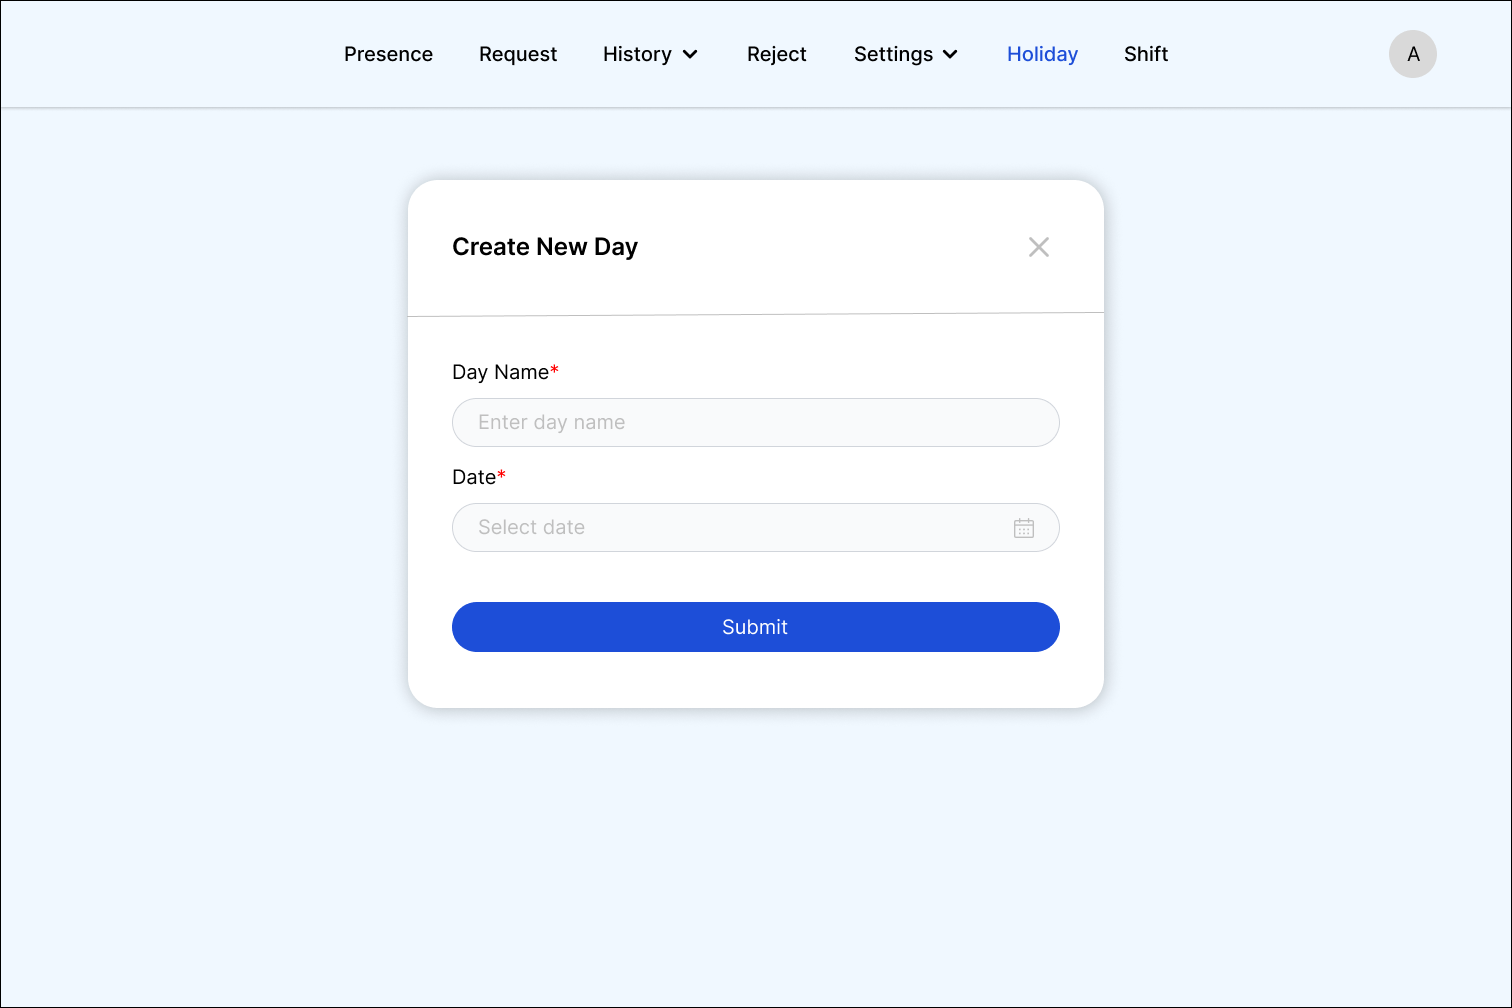
\includegraphics[width=13cm]{Gambar/bab2/mockups/menu-tambah-hari-libur.png}
	\caption{\textit{Mockup} Menu Tambah Hari Libur}
	\label{fig:mockup-menu-tambah-hari-libur}
\end{figure}
\FloatBarrier

\begin{figure}[H]
	\centering
	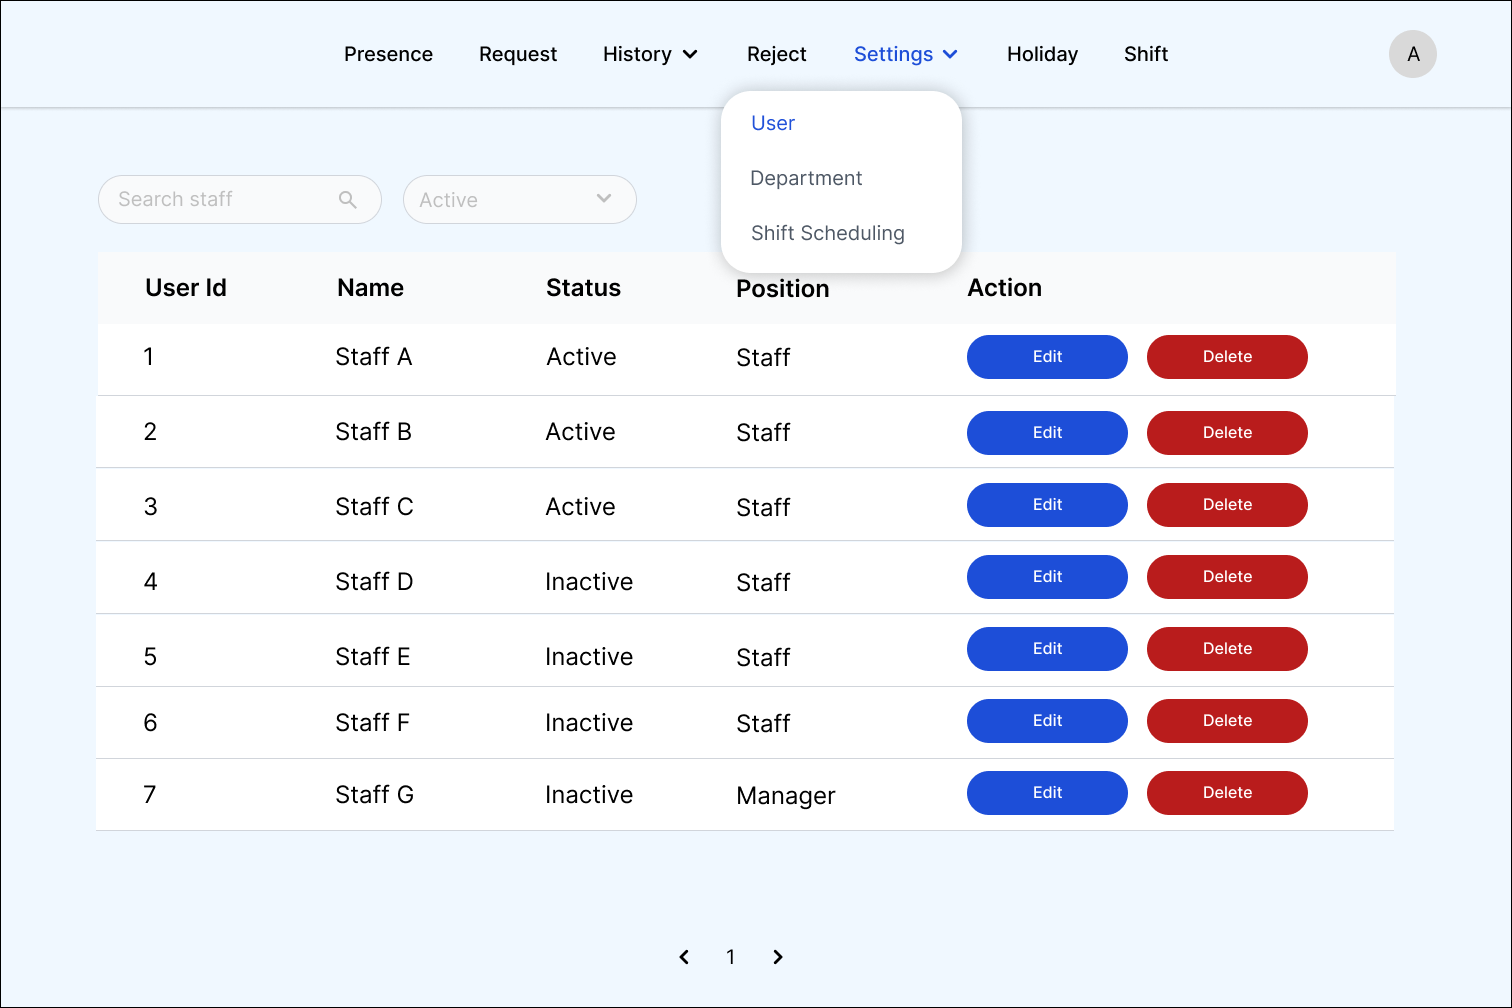
\includegraphics[width=13cm]{Gambar/bab2/mockups/menu-user.png}
	\caption{\textit{Mockup} Menu \textit{User}}
	\label{fig:mockup-menu-user}
\end{figure}
\FloatBarrier

\begin{figure}[H]
	\centering
	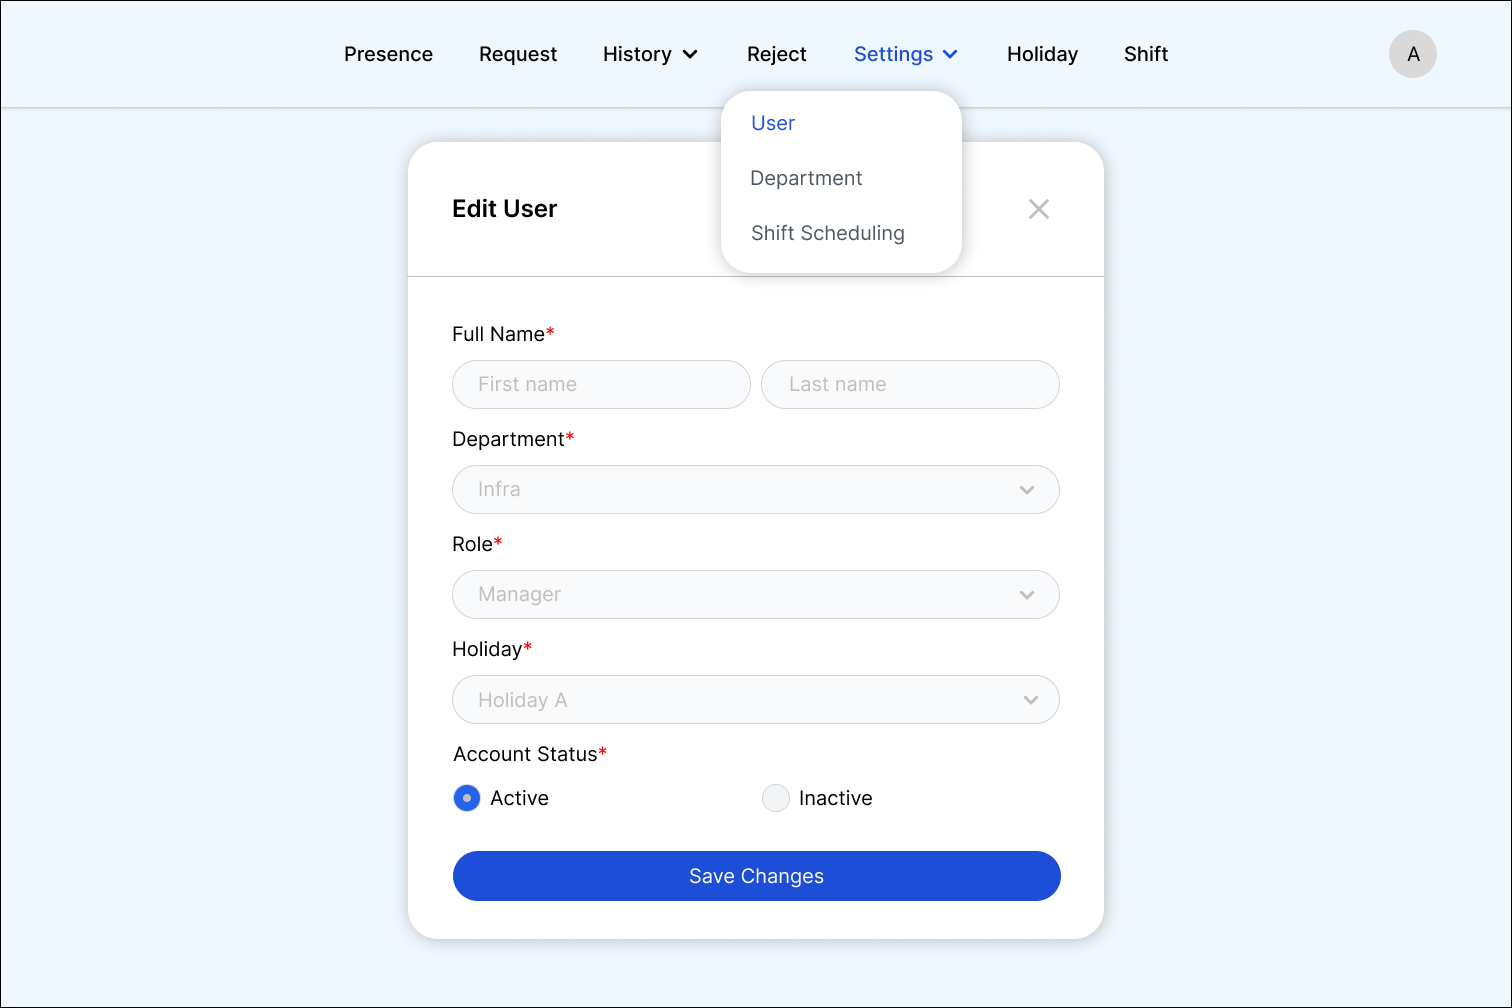
\includegraphics[width=13cm]{Gambar/bab2/mockups/menu-edit-user.png}
	\caption{\textit{Mockup} Menu \textit{Edit User}}
	\label{fig:mockup-menu-edit-user}
\end{figure}
\FloatBarrier

\begin{figure}[H]
	\centering
	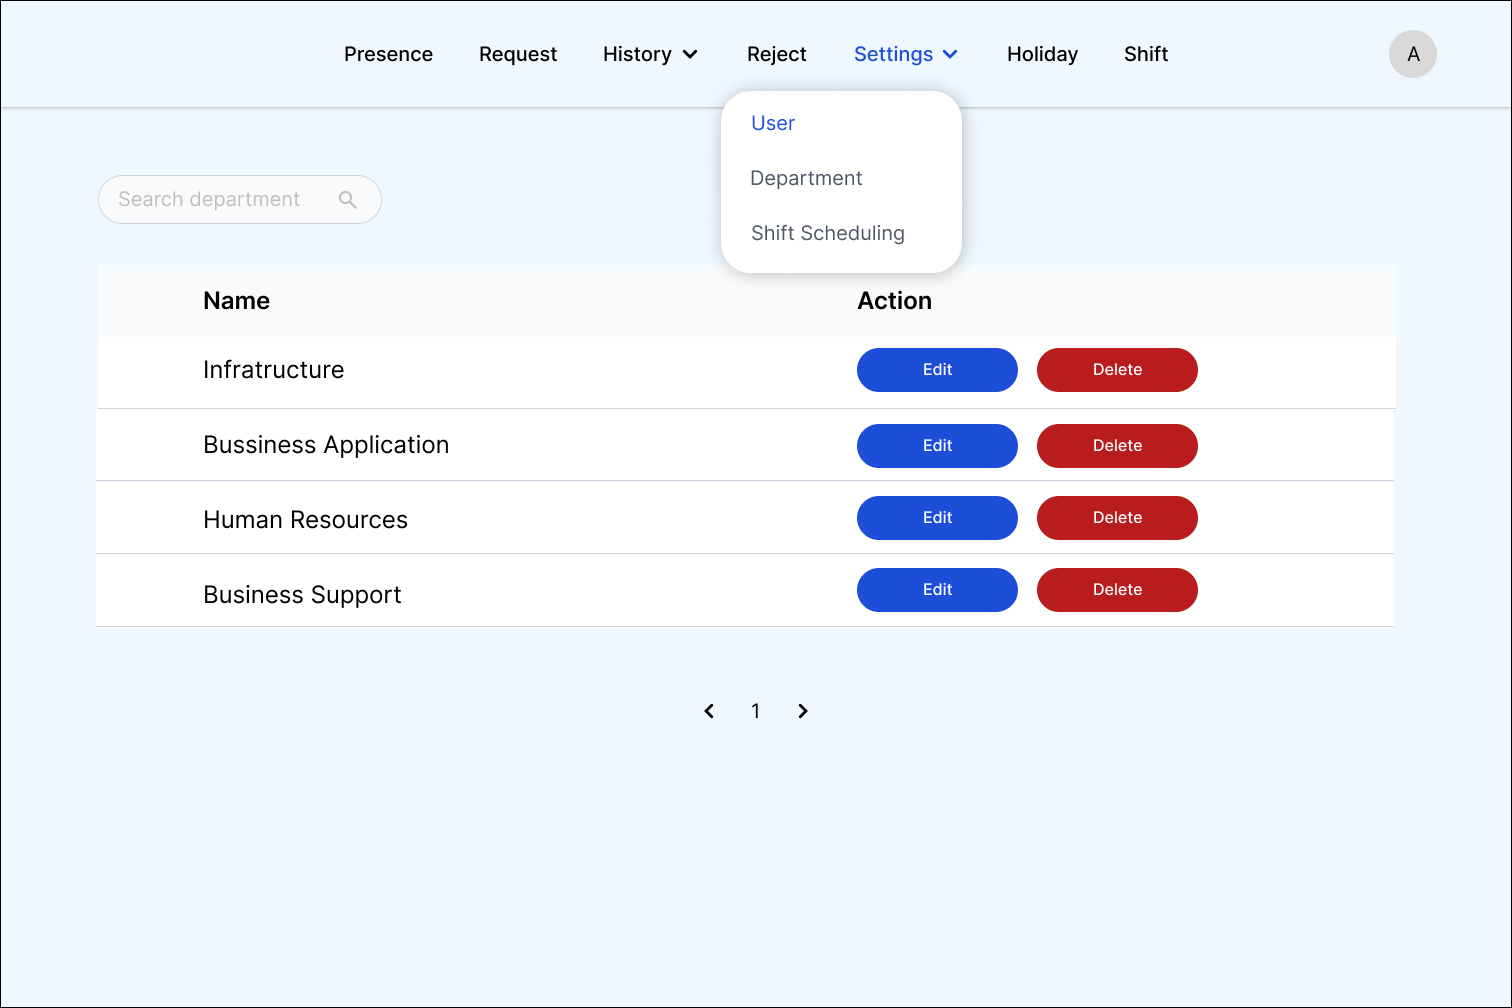
\includegraphics[width=13cm]{Gambar/bab2/mockups/menu-department.png}
	\caption{\textit{Mockup} Menu \textit{Department}}
	\label{fig:mockup-menu-department}
\end{figure}
\FloatBarrier

\begin{figure}[H]
	\centering
	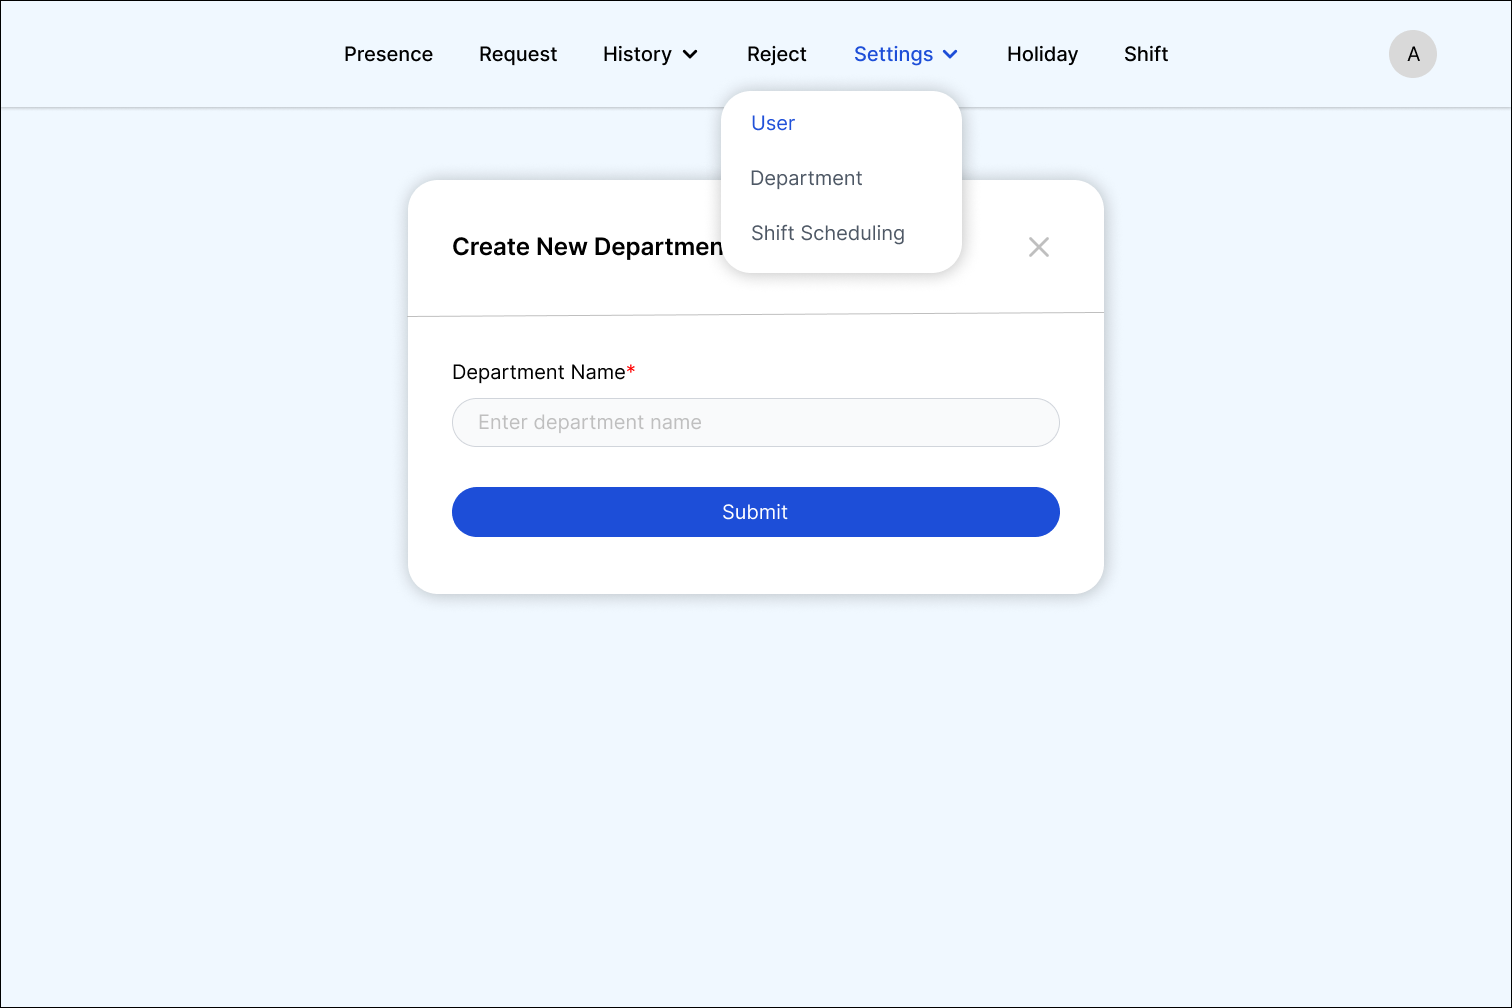
\includegraphics[width=13cm]{Gambar/bab2/mockups/menu-tambah-department.png}
	\caption{\textit{Mockup} Menu Tambah \textit{Department}}
	\label{fig:mockup-menu-tambah-department}
\end{figure}
\FloatBarrier

\begin{figure}[H]
	\centering
	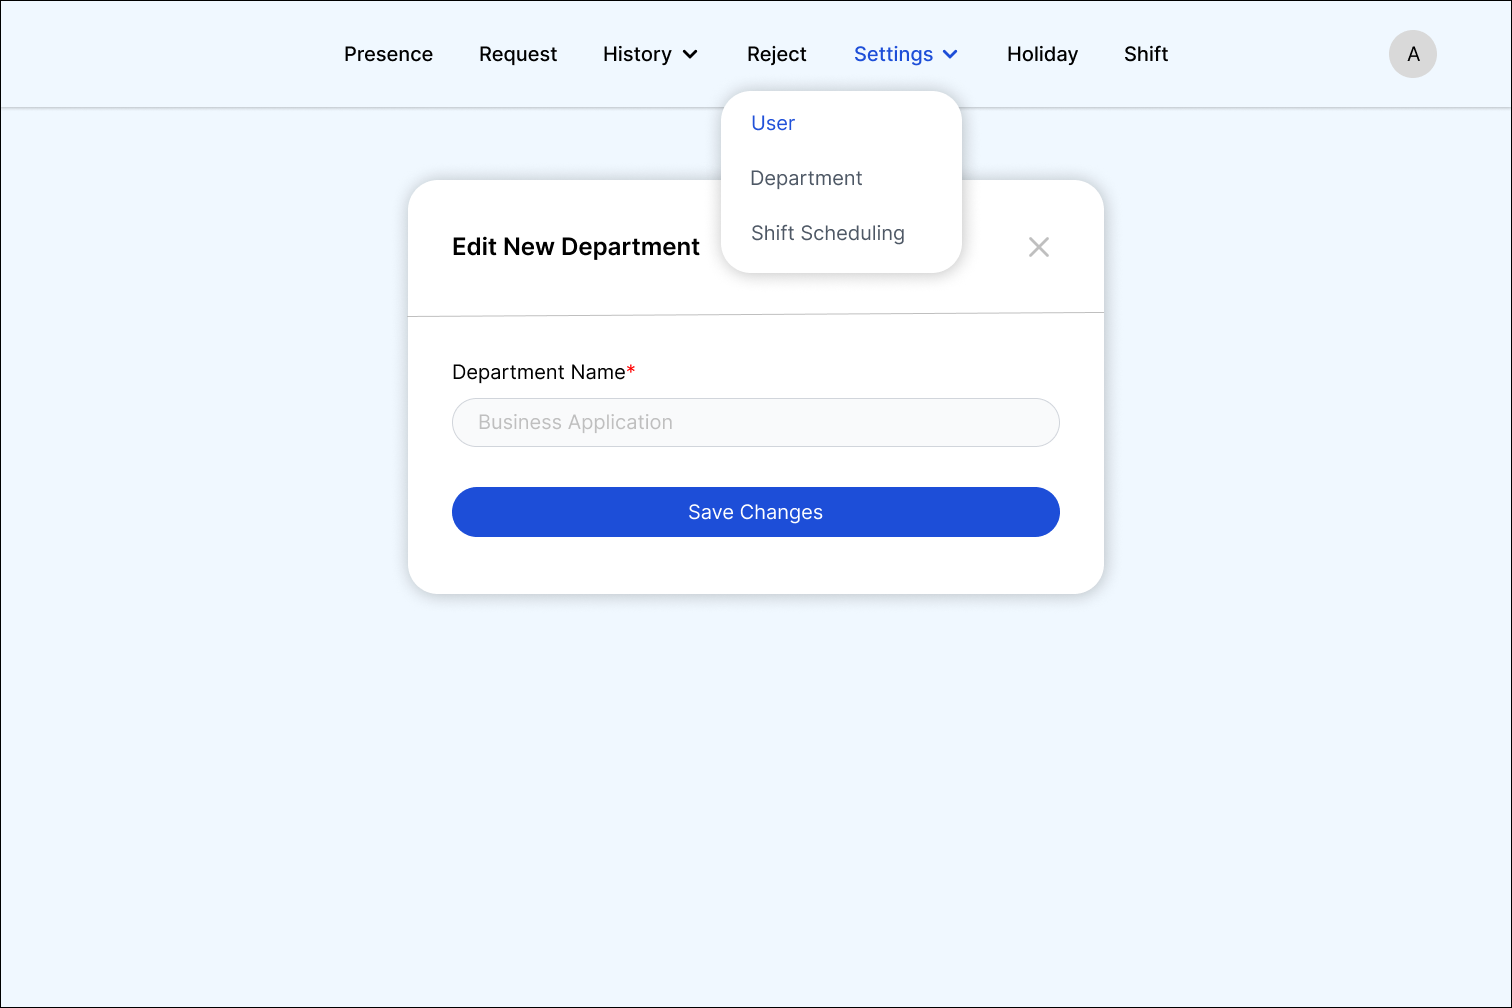
\includegraphics[width=13cm]{Gambar/bab2/mockups/menu-edit-department.png}
	\caption{\textit{Mockup} Menu \textit{Edit} \textit{Department}}
	\label{fig:mockup-menu-edit-department}
\end{figure}
\FloatBarrier

\begin{figure}[H]
	\centering
	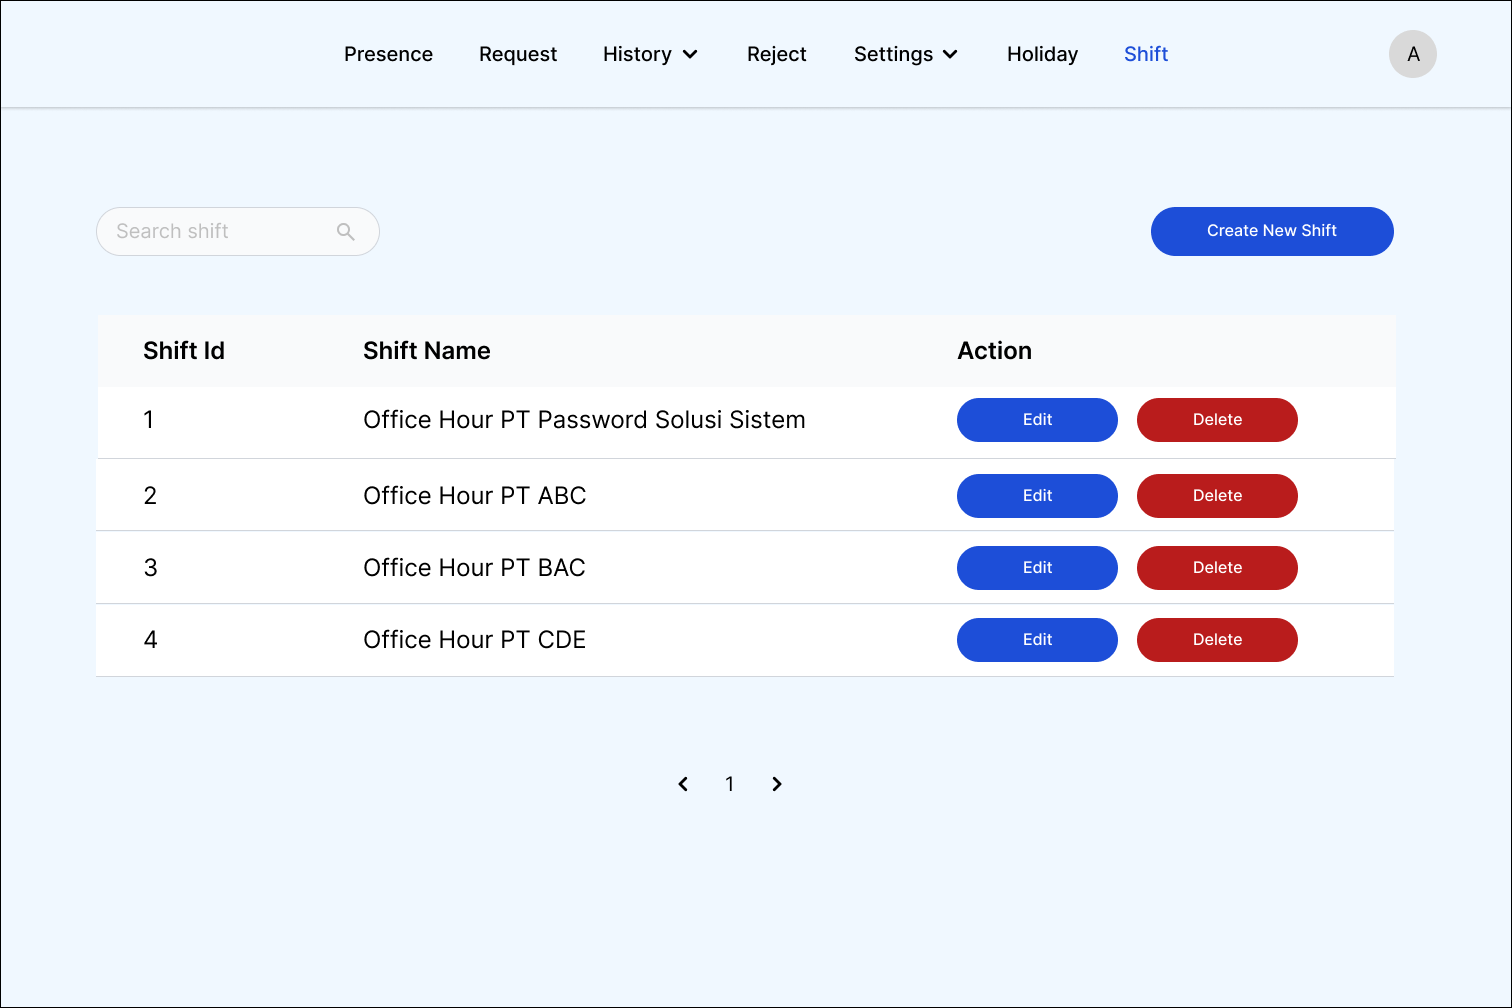
\includegraphics[width=13cm]{Gambar/bab2/mockups/menu-shift.png}
	\caption{\textit{Mockup} Menu \textit{Shift}}
	\label{fig:mockup-menu-shift}
\end{figure}
\FloatBarrier

\begin{figure}[H]
	\centering
	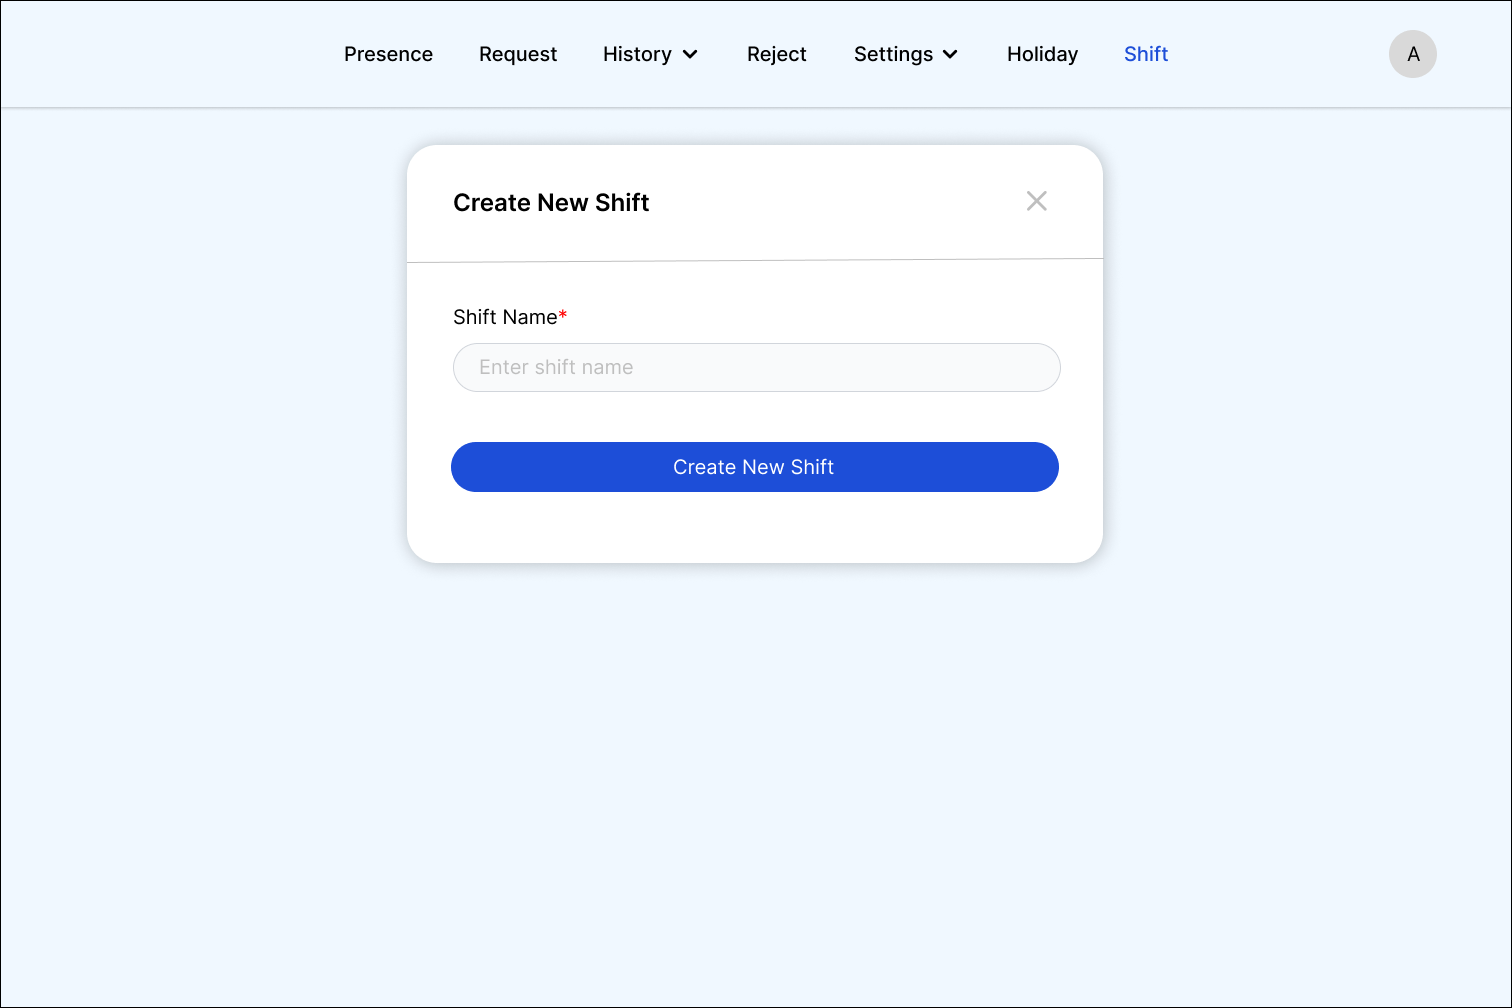
\includegraphics[width=13cm]{Gambar/bab2/mockups/menu-tambah-shift.png}
	\caption{\textit{Mockup} Menu Tambah \textit{Shift}}
	\label{fig:mockup-menu-tambah-shift}
\end{figure}
\FloatBarrier

\begin{figure}[H]
	\centering
	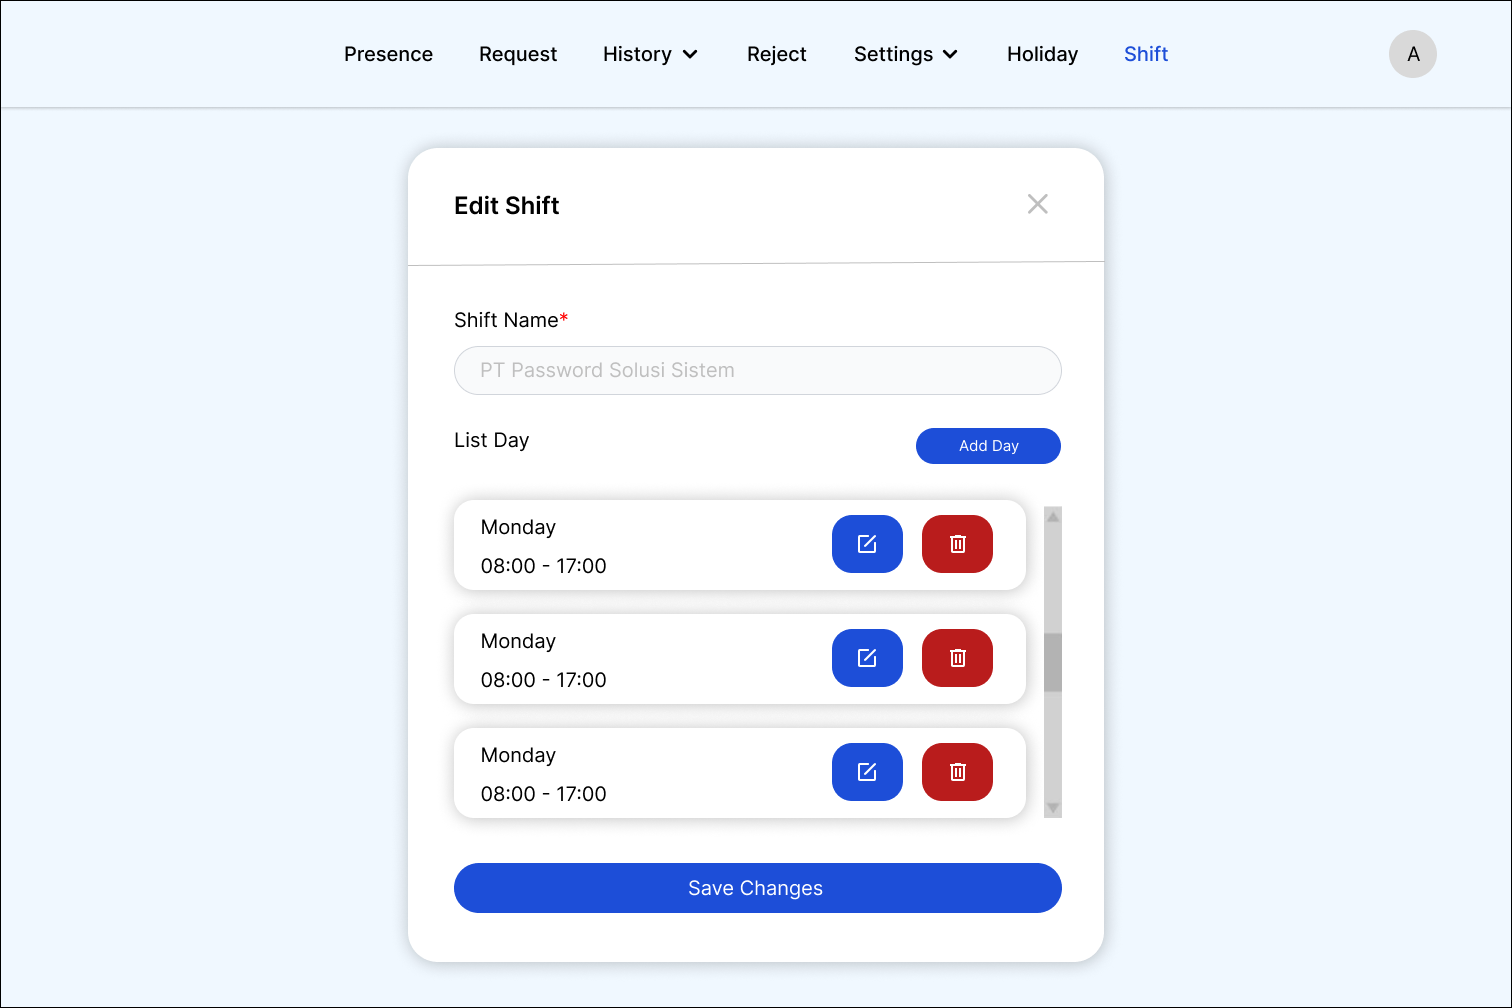
\includegraphics[width=13cm]{Gambar/bab2/mockups/menu-edit-shift.png}
	\caption{\textit{Mockup} Menu Hari \textit{Shift}}
	\label{fig:mockup-menu-edit-shift}
\end{figure}
\FloatBarrier

\begin{figure}[H]
	\centering
	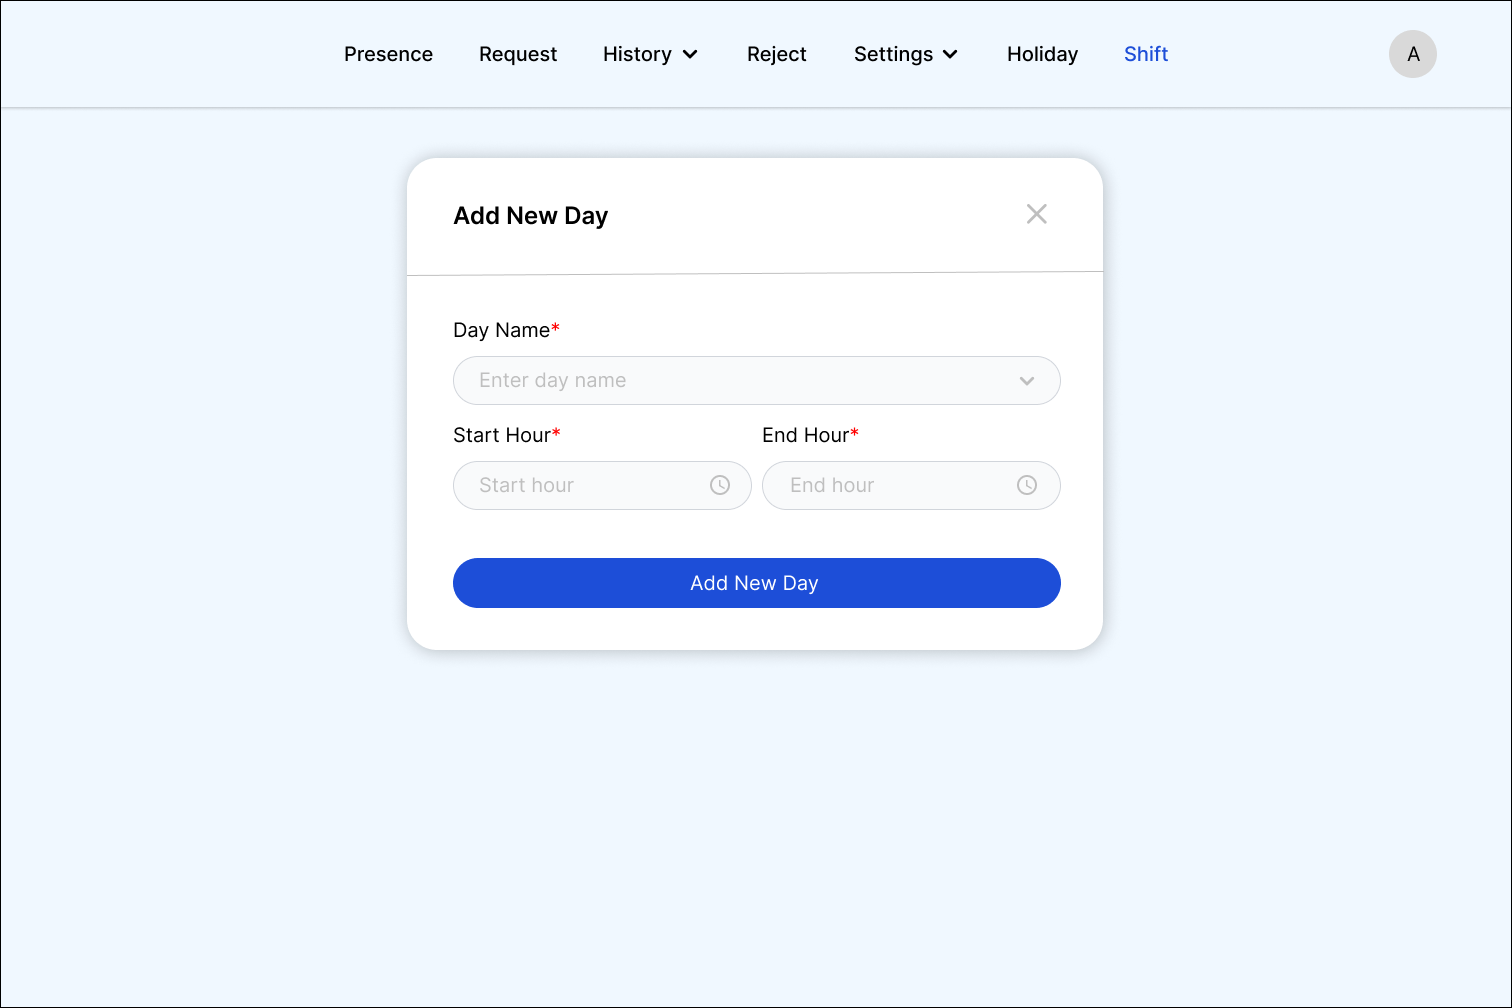
\includegraphics[width=13cm]{Gambar/bab2/mockups/menu-tambah-hari.png}
	\caption{\textit{Mockup} Menu Tambah Hari \textit{Shift}}
	\label{fig:mockup-menu-tambah-hari}
\end{figure}
\FloatBarrier

\begin{figure}[H]
	\centering
	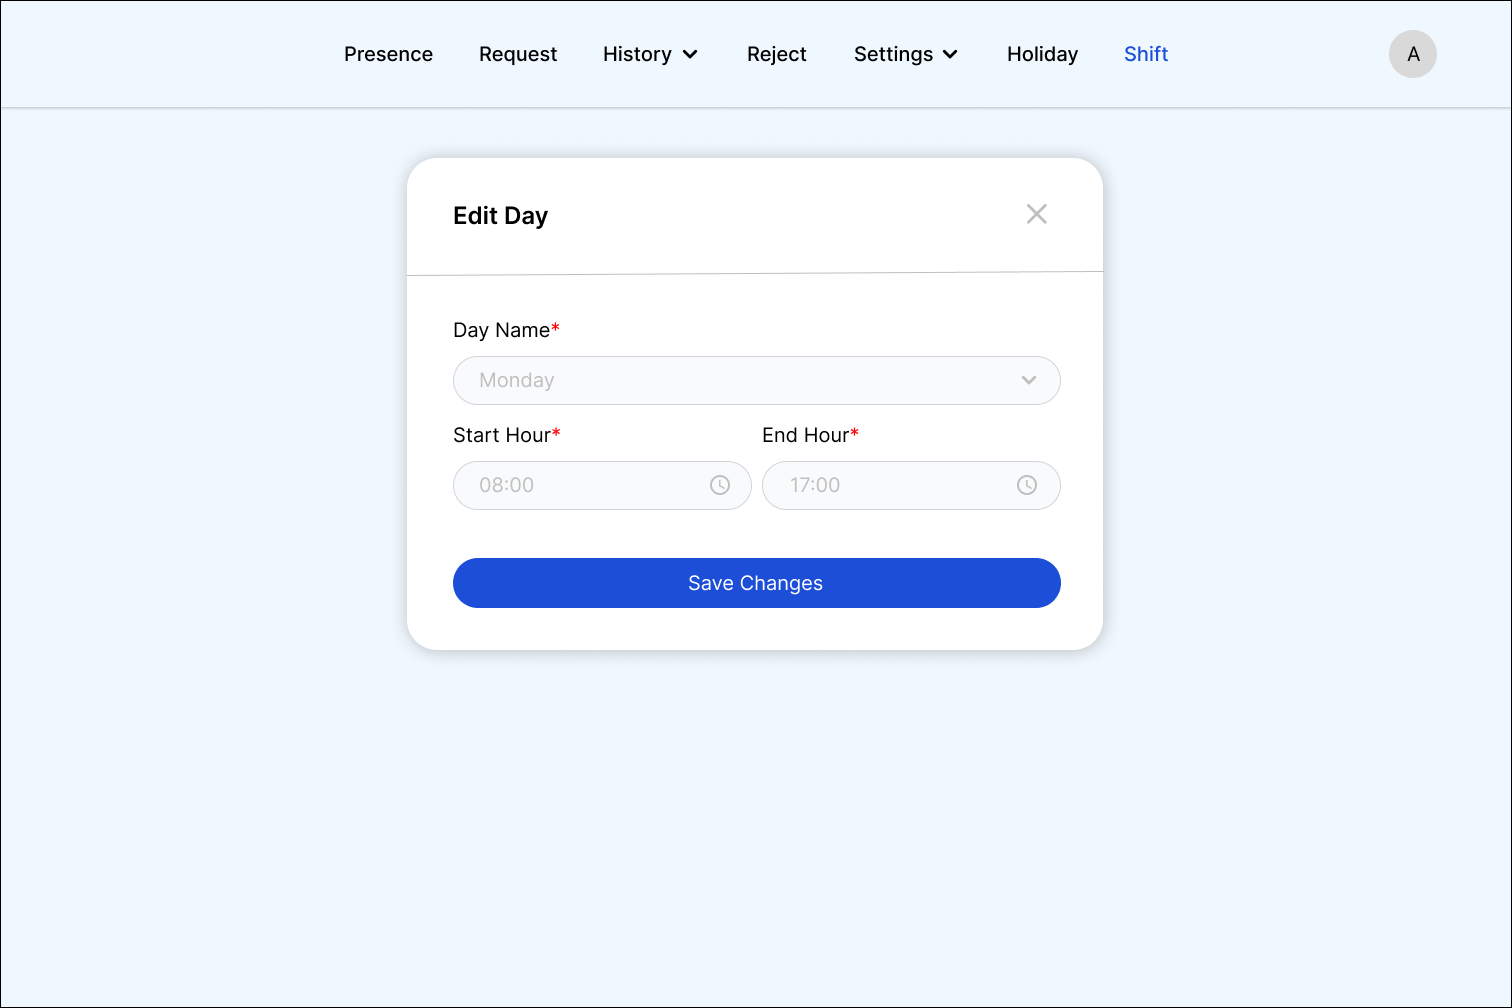
\includegraphics[width=13cm]{Gambar/bab2/mockups/menu-edit-hari.png}
	\caption{\textit{Mockup} Menu \textit{Edit} Hari \textit{Shift}}
	\label{fig:mockup-menu-edit-hari}
\end{figure}
\FloatBarrier

\begin{figure}[H]
	\centering
	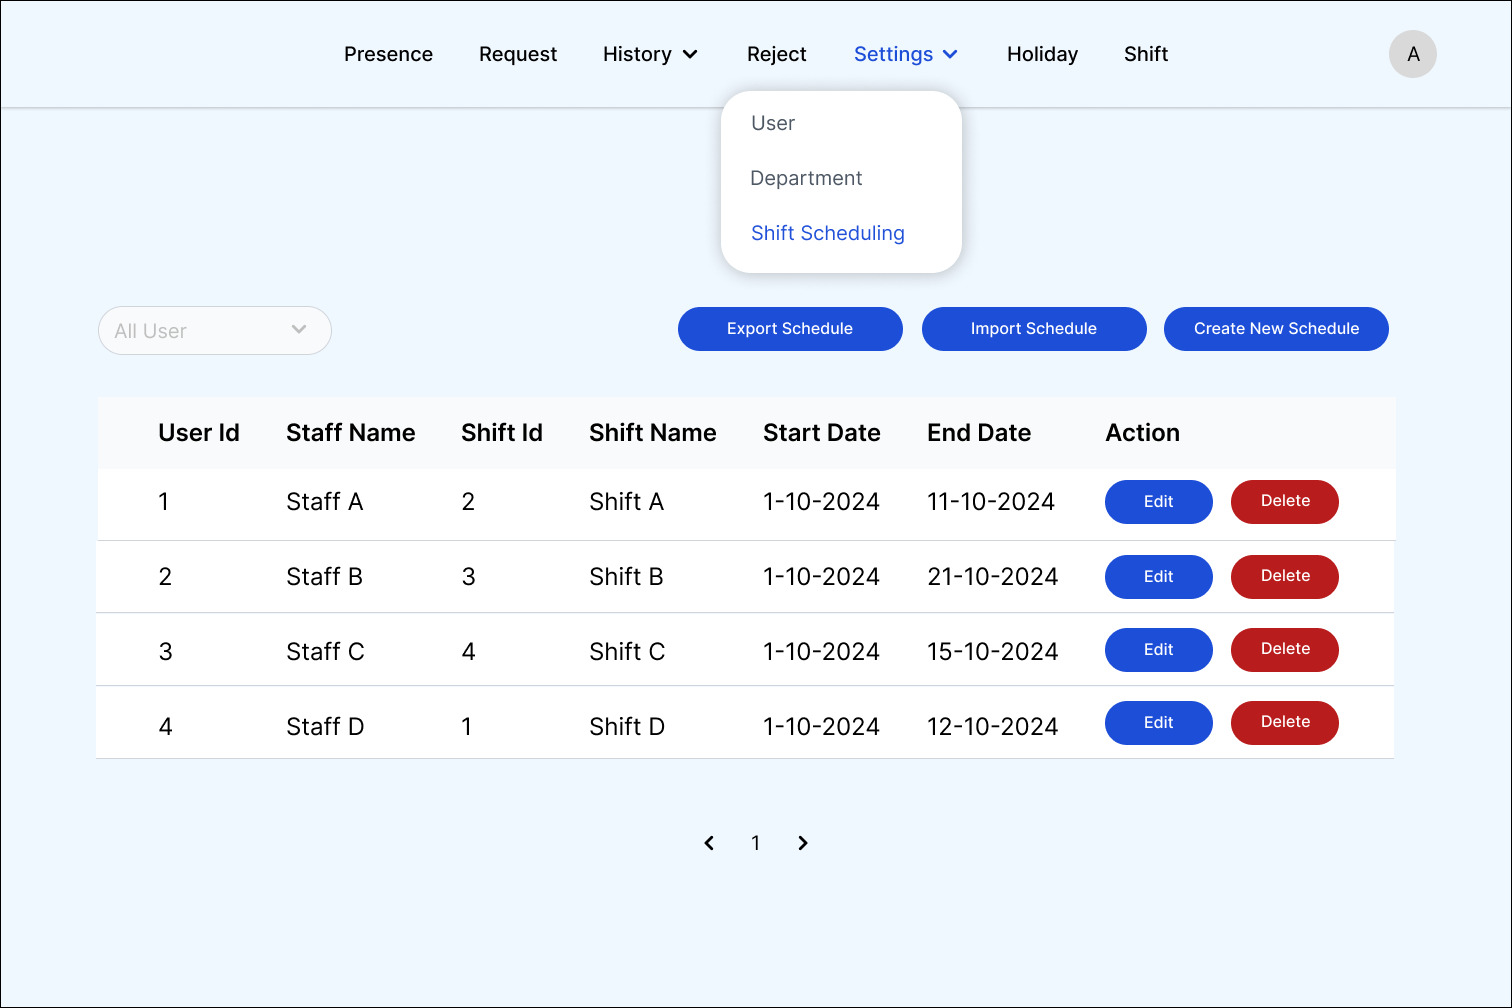
\includegraphics[width=13cm]{Gambar/bab2/mockups/menu-shift-scheduling.png}
	\caption{\textit{Mockup} Menu \textit{Shift Scheduling}}
	\label{fig:mockup-menu-scheduling-shift}
\end{figure}
\FloatBarrier

\begin{figure}[H]
	\centering
	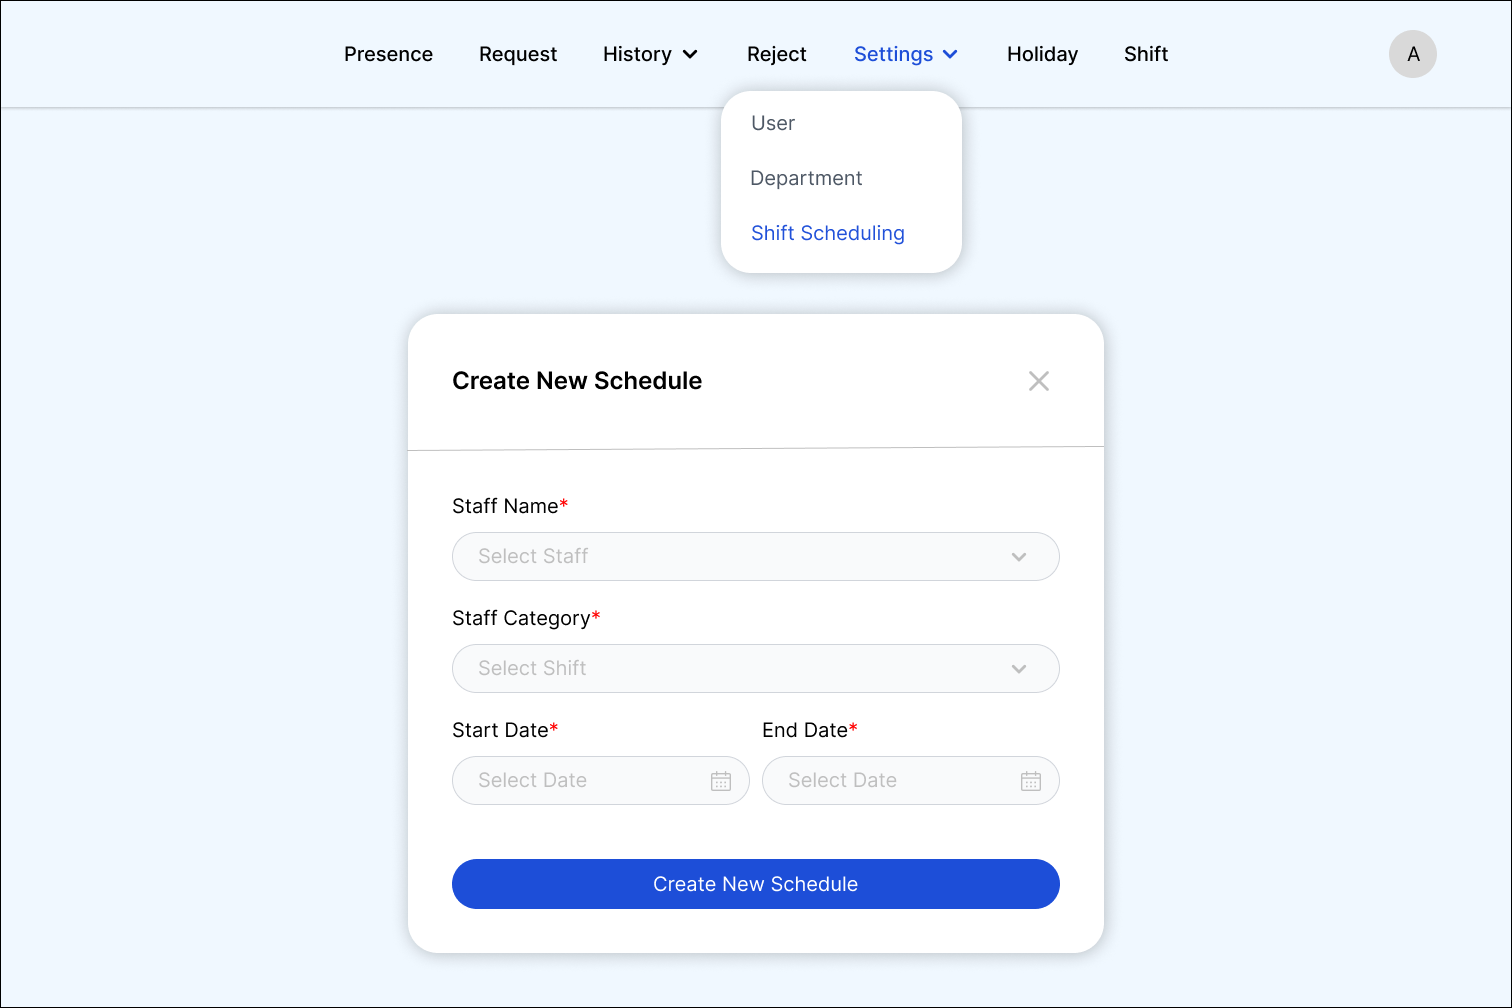
\includegraphics[width=13cm]{Gambar/bab2/mockups/menu-tambah-shift-scheduling.png}
	\caption{\textit{Mockup} Menu Tambah \textit{Shift Scheduling}}
	\label{fig:mockup-menu-tambah-scheduling-shift}
\end{figure}
\FloatBarrier

\begin{figure}[H]
	\centering
	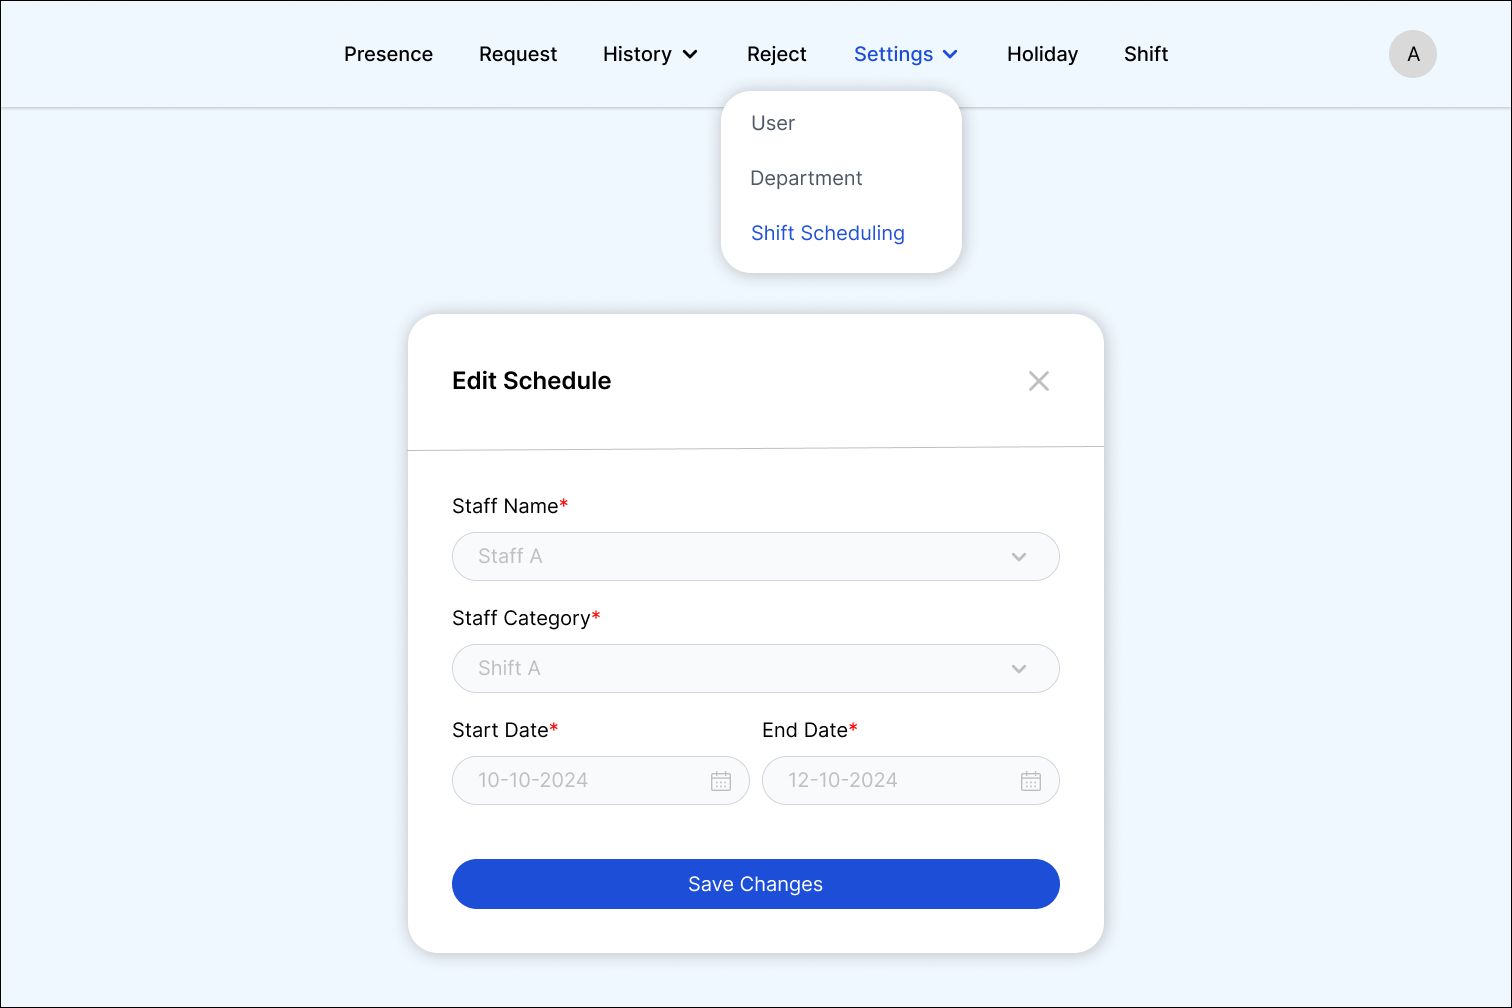
\includegraphics[width=13cm]{Gambar/bab2/mockups/menu-edit-shift-scheduling.png}
	\caption{\textit{Mockup} Menu \textit{Edit} \textit{Shift Scheduling}}
	\label{fig:mockup-menu-edit-scheduling-shift}
\end{figure}
\FloatBarrier

\begin{figure}[H]
	\centering
	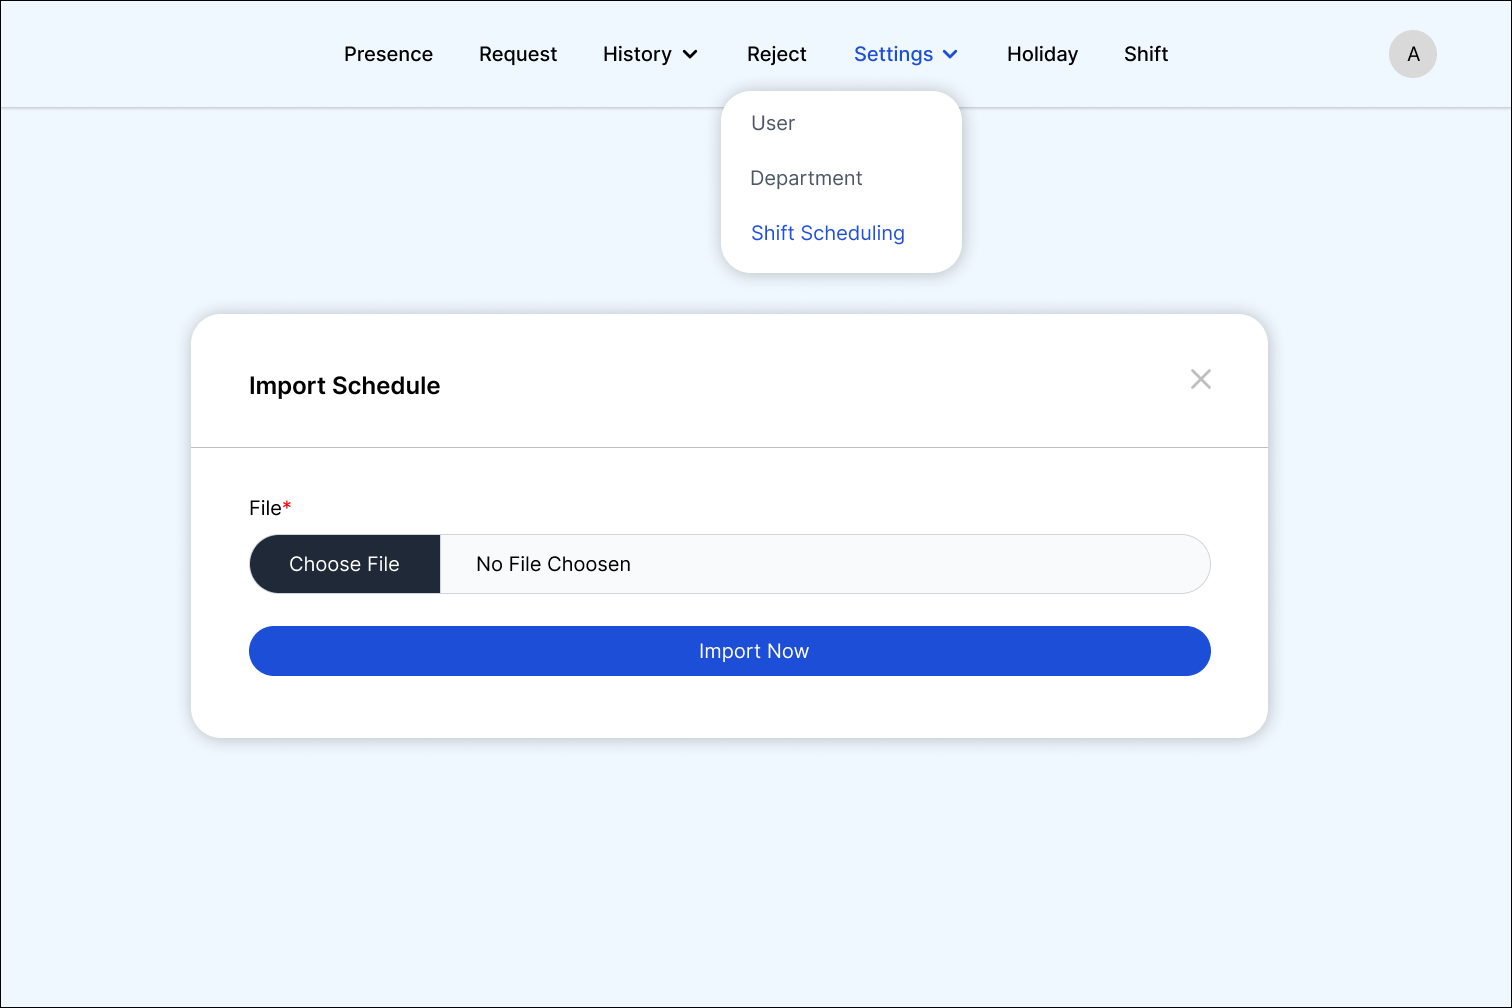
\includegraphics[width=13cm]{Gambar/bab2/mockups/menu-import-shift-scheduling.png}
	\caption{\textit{Mockup} Menu \textit{Import} \textit{Shift Scheduling}}
	\label{fig:mockup-menu-import-scheduling-shift}
\end{figure}
\FloatBarrier
\pagebreak

\nextappendix
\section*{Lampiran \theappendixletter: \textit{User Manual} Aplikasi Presensi \textit{Online}
\label{sec:user-manual-aplikasi-presensi-online}}
\addcontentsline{toc}{section}{Lampiran \theappendixletter: \textit{User Manual} Aplikasi Presensi \textit{Online}} 
%%%%%%%%%%%%%%%
% \setcounter{figure}{0}
% \setcounter{page}{1}
% \pagenumbering{gobble}
%%%%%%%%%%%%%%%

\begin{enumerate}
    \item Mengakses Aplikasi\label{item:mengakses-aplikasi}
    \begin{enumerate}
        \item Membuka aplikasi \textit{browser}, kemudian memasukkan tautan URL aplikasi presensi \textit{online}. \textbf{\ref{fig:memasukkan-tautan-url-melalui-browser}} menunjukkan cara memasukkan tautan URL melalui \textit{browser}.
        \begin{figure}[!htbp]
    	\centering
    	
\includegraphics[width=10cm]{Gambar/bab3/user-manual/user-manual-enter-link.png}
    	\caption{Memasukkan Tautan URL Melalui \textit{Browser}}
    	\label{fig:memasukkan-tautan-url-melalui-browser}
        \end{figure}
        \FloatBarrier

        \item Setelah memasukkan tautan URL, maka halaman akan otomatis teralihkan ke halaman \textit{login} pada aplikasi presensi \textit{online}. \textbf{\ref{fig:user-manual-halaman-login}} menunjukkan tampilan \textit{login} pada aplikasi presensi \textit{online}.
        \begin{figure}[!htbp]
    	\centering
    	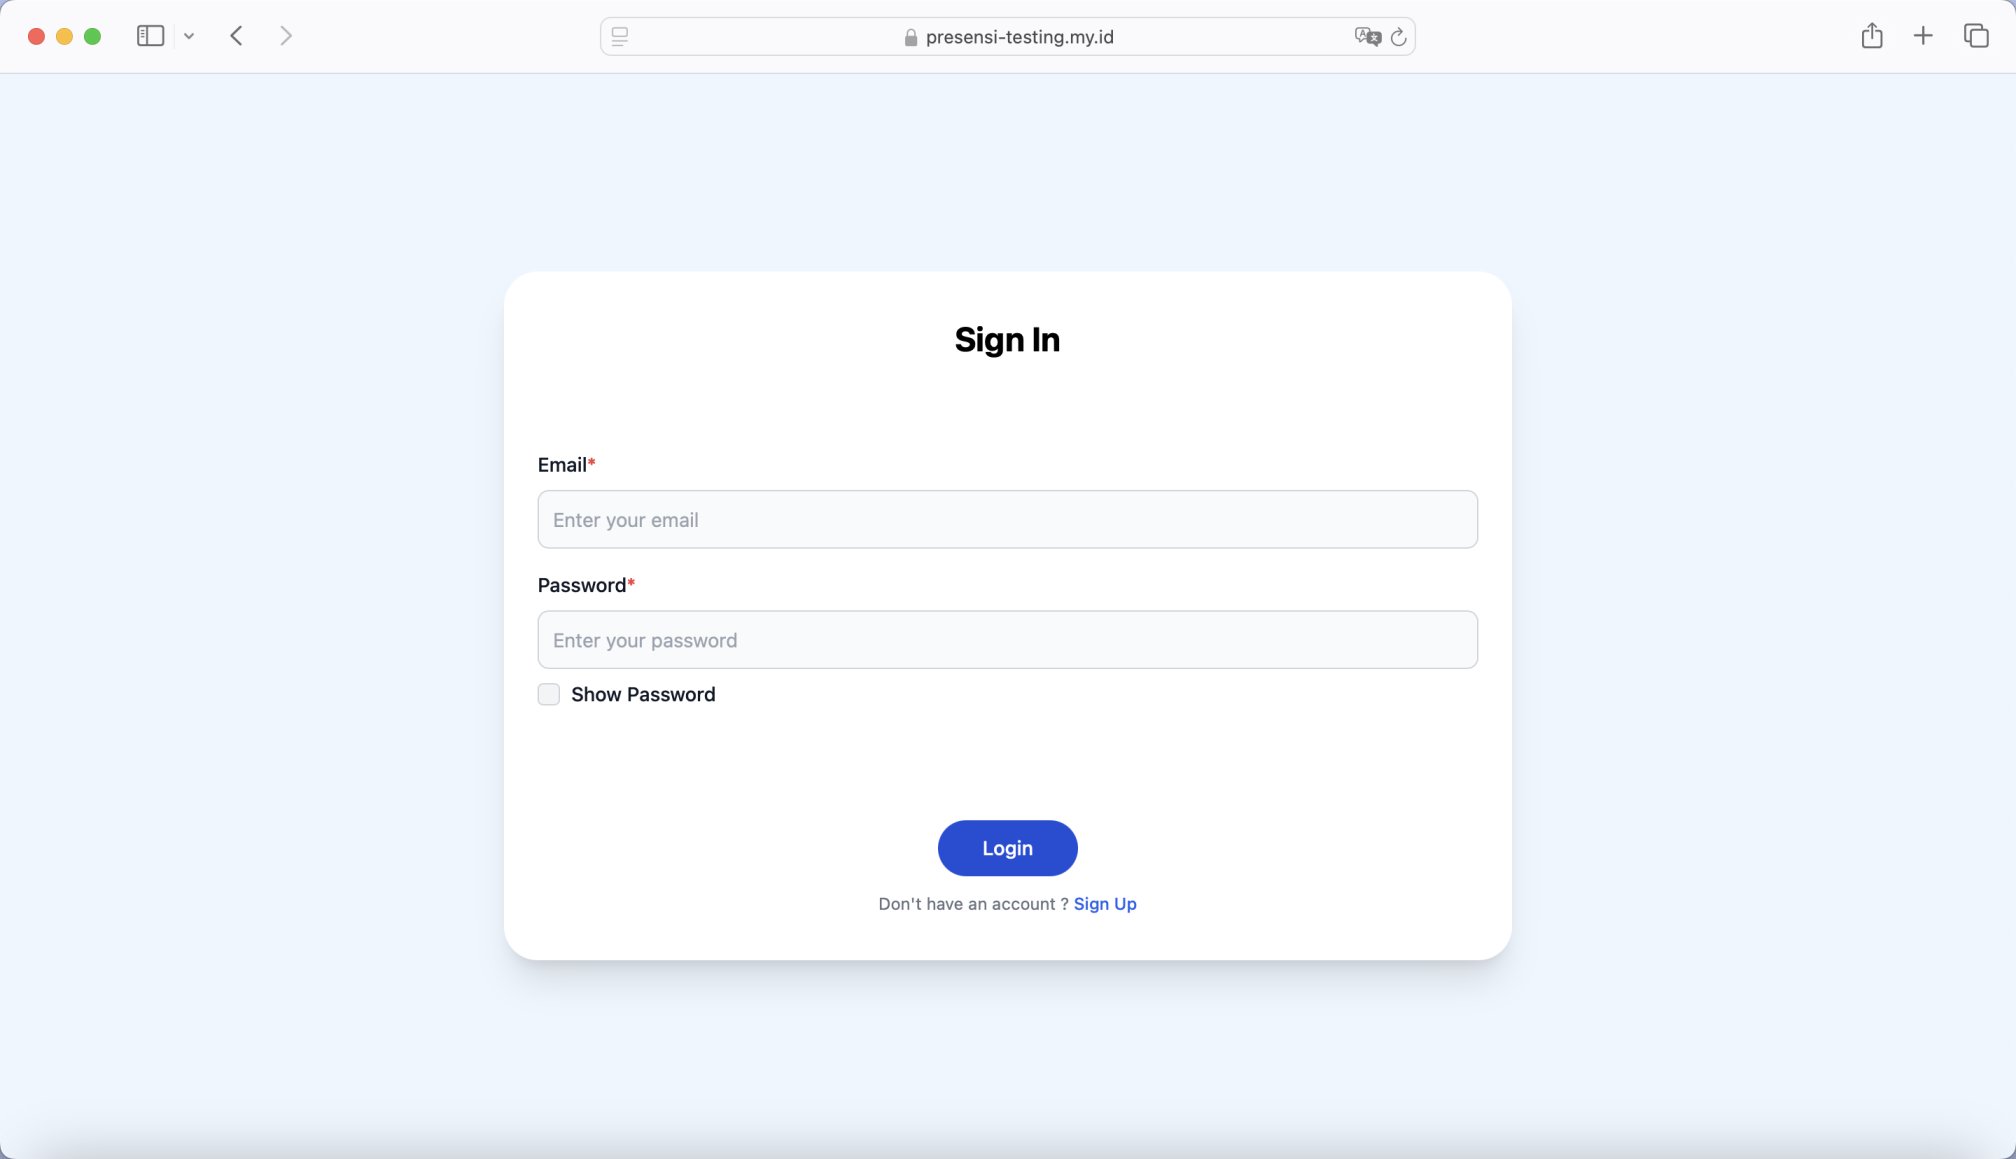
\includegraphics[width=10cm]{Gambar/bab3/user-manual/user-manual-halaman-login.png}
    	\caption{Tampilan Halaman \textit{Login}}
    	\label{fig:user-manual-halaman-login}
        \end{figure}
        \FloatBarrier
    \end{enumerate}

    \item Melakukan \textit{Login}\label{item:melakukan-login}
    \begin{enumerate}
        \item Mengakses aplikasi presensi \textit{online} yang terdapat pada \textbf{Manual \ref{item:mengakses-aplikasi}}.

        \item Mengisi seluruh \textit{input form} pada halaman \textit{login}, kemudian menekan tombol \textit{"Login"}. \textbf{\ref{fig:user-manual-halaman-login}} menunjukkan tampilan halaman \textit{login}.

        \item Halaman akan dialihkan ke halaman utama jika berhasil \textit{login}. \textbf{\ref{fig:user-manual-halaman-utama}} menunjukkan tampilan halaman utama aplikasi presensi \textit{online} ketika berhasil \textit{login}.

        \begin{figure}[!htbp]
    	\centering
    	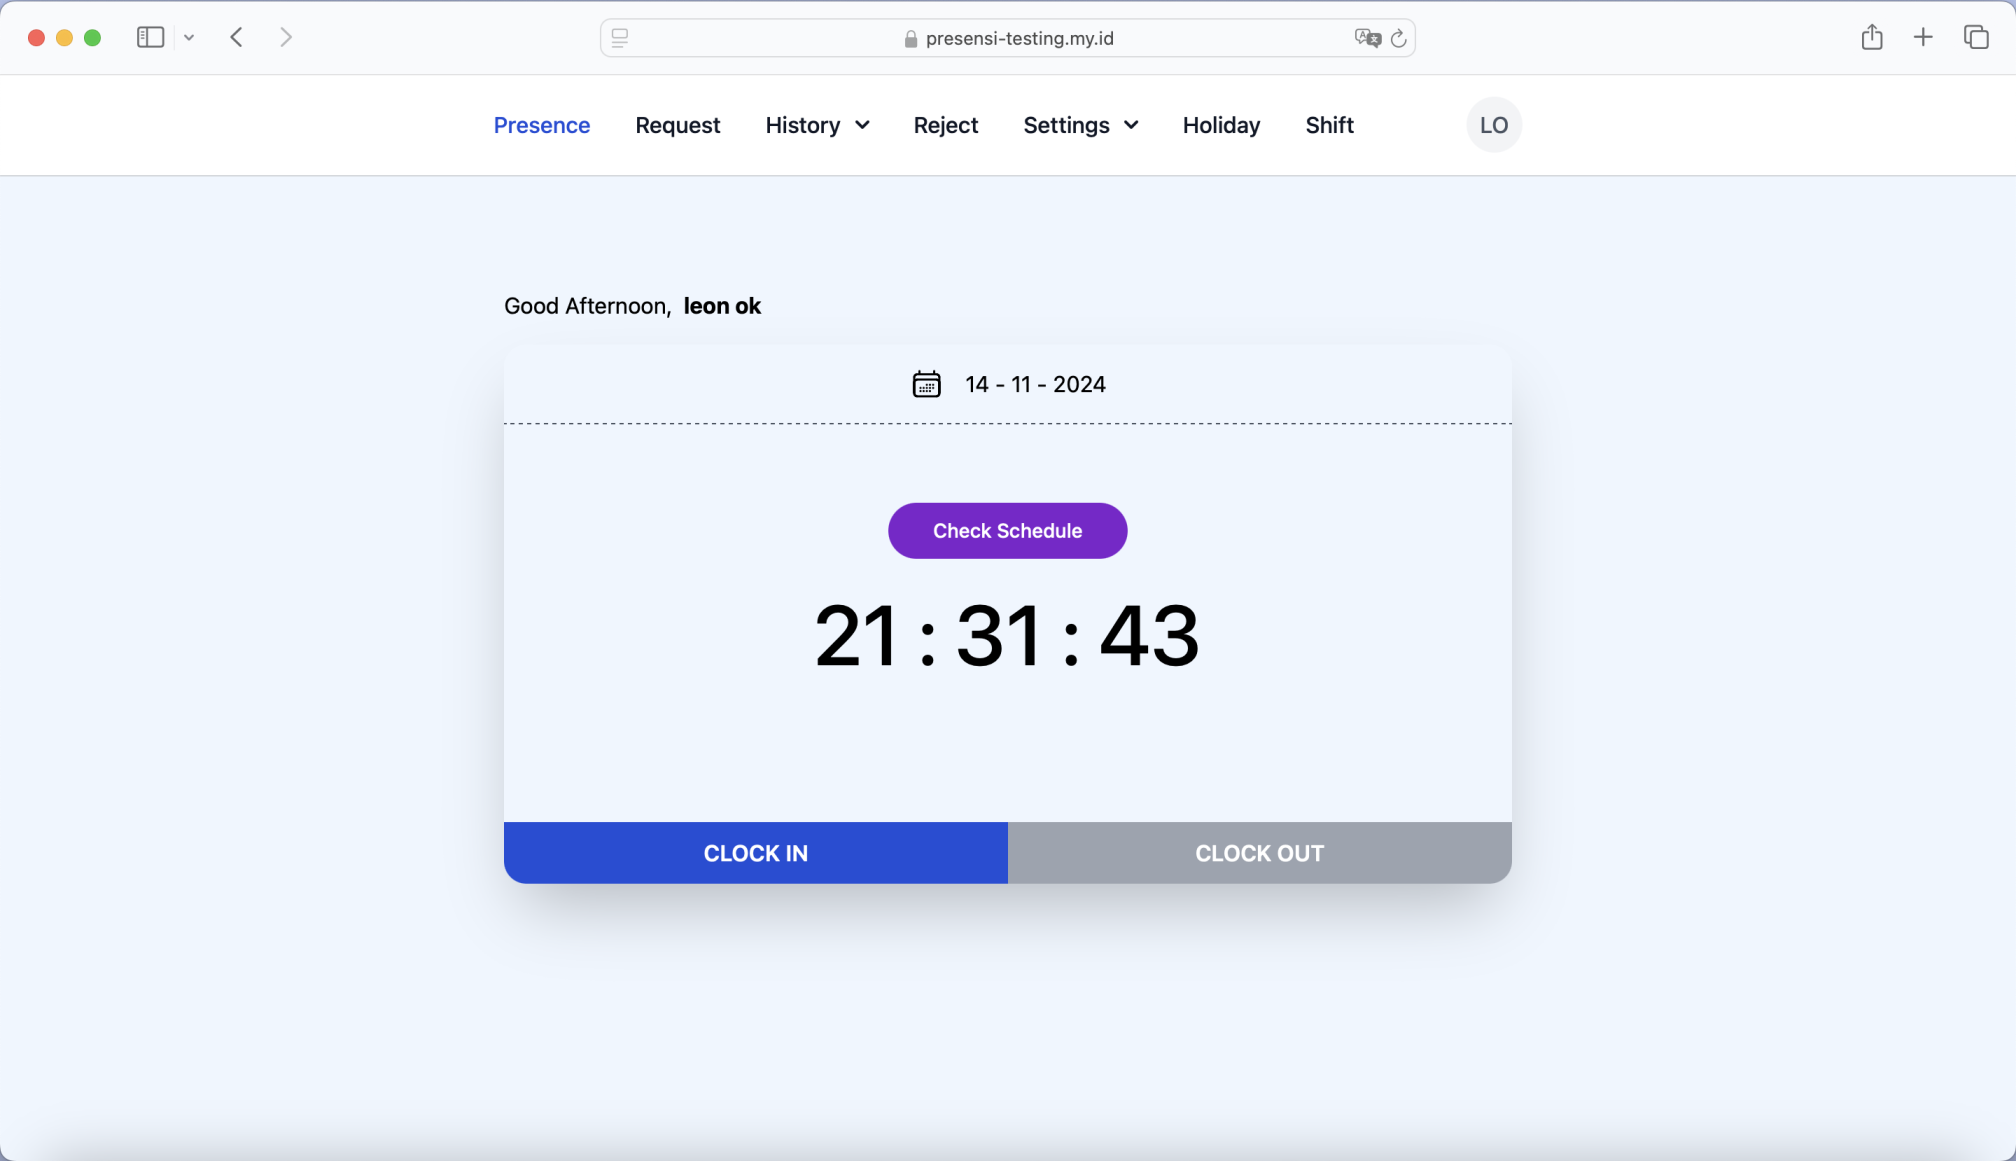
\includegraphics[width=10cm]{Gambar/bab3/user-manual/user-manual-halaman-utama.png}
    	\caption{Halaman Utama}
    	\label{fig:user-manual-halaman-utama}
        \end{figure}
        \FloatBarrier
    \end{enumerate}

    \item Melakukan Registrasi Akun
    \begin{enumerate}
        \item Mengakses aplikasi presensi \textit{online} yang terdapat pada \textbf{Manual \ref{item:mengakses-aplikasi}}.
        \item Menekan tombol \textit{"Sign Up"} pada halaman \textit{login}. \textbf{\ref{fig:user-manual-tombol-sign-up}} terdapat tombol \textit{"Sign Up"} yang terletak di paling bawah halaman.
        \item Mengisi seluruh \textit{input form} yang ada pada halaman registrasi akun dan menekan tombol \textit{"Register"}. \textbf{\ref{fig:user-manual-halaman-sign-up}} menunjukkan halaman registrasi akun.
        \item Sistem akan mengirimkan 6 digit kode OTP ke \textit{email} pengguna, memasukkan kode OTP ke dalam modal verifikasi \textit{email}. \textbf{\ref{fig:user-manual-verifikasi-email}} menunjukkan modal untuk verifikasi \textit{email} pada akun.
        \item Setelah memasukkan kode verifikasi \textit{email} dengan benar maka akan muncul pesan berhasil. \textbf{\ref{fig:user-manual-pesan-berhasil-verifikasi}} menunjukkan \textit{pop up} pesan berhasil verifikasi \textit{email} pada akun.
        \begin{figure}[!htbp]
    	\centering
    	
\includegraphics[width=10cm]{Gambar/bab3/user-manual/user-manual-tombol-sign-up.png}
    	\caption{Tombol \textit{Sign Up} Pada Halaman \textit{Login}}
    	\label{fig:user-manual-tombol-sign-up}
        \end{figure}
        \FloatBarrier

        \begin{figure}[!htbp]
    	\centering
    	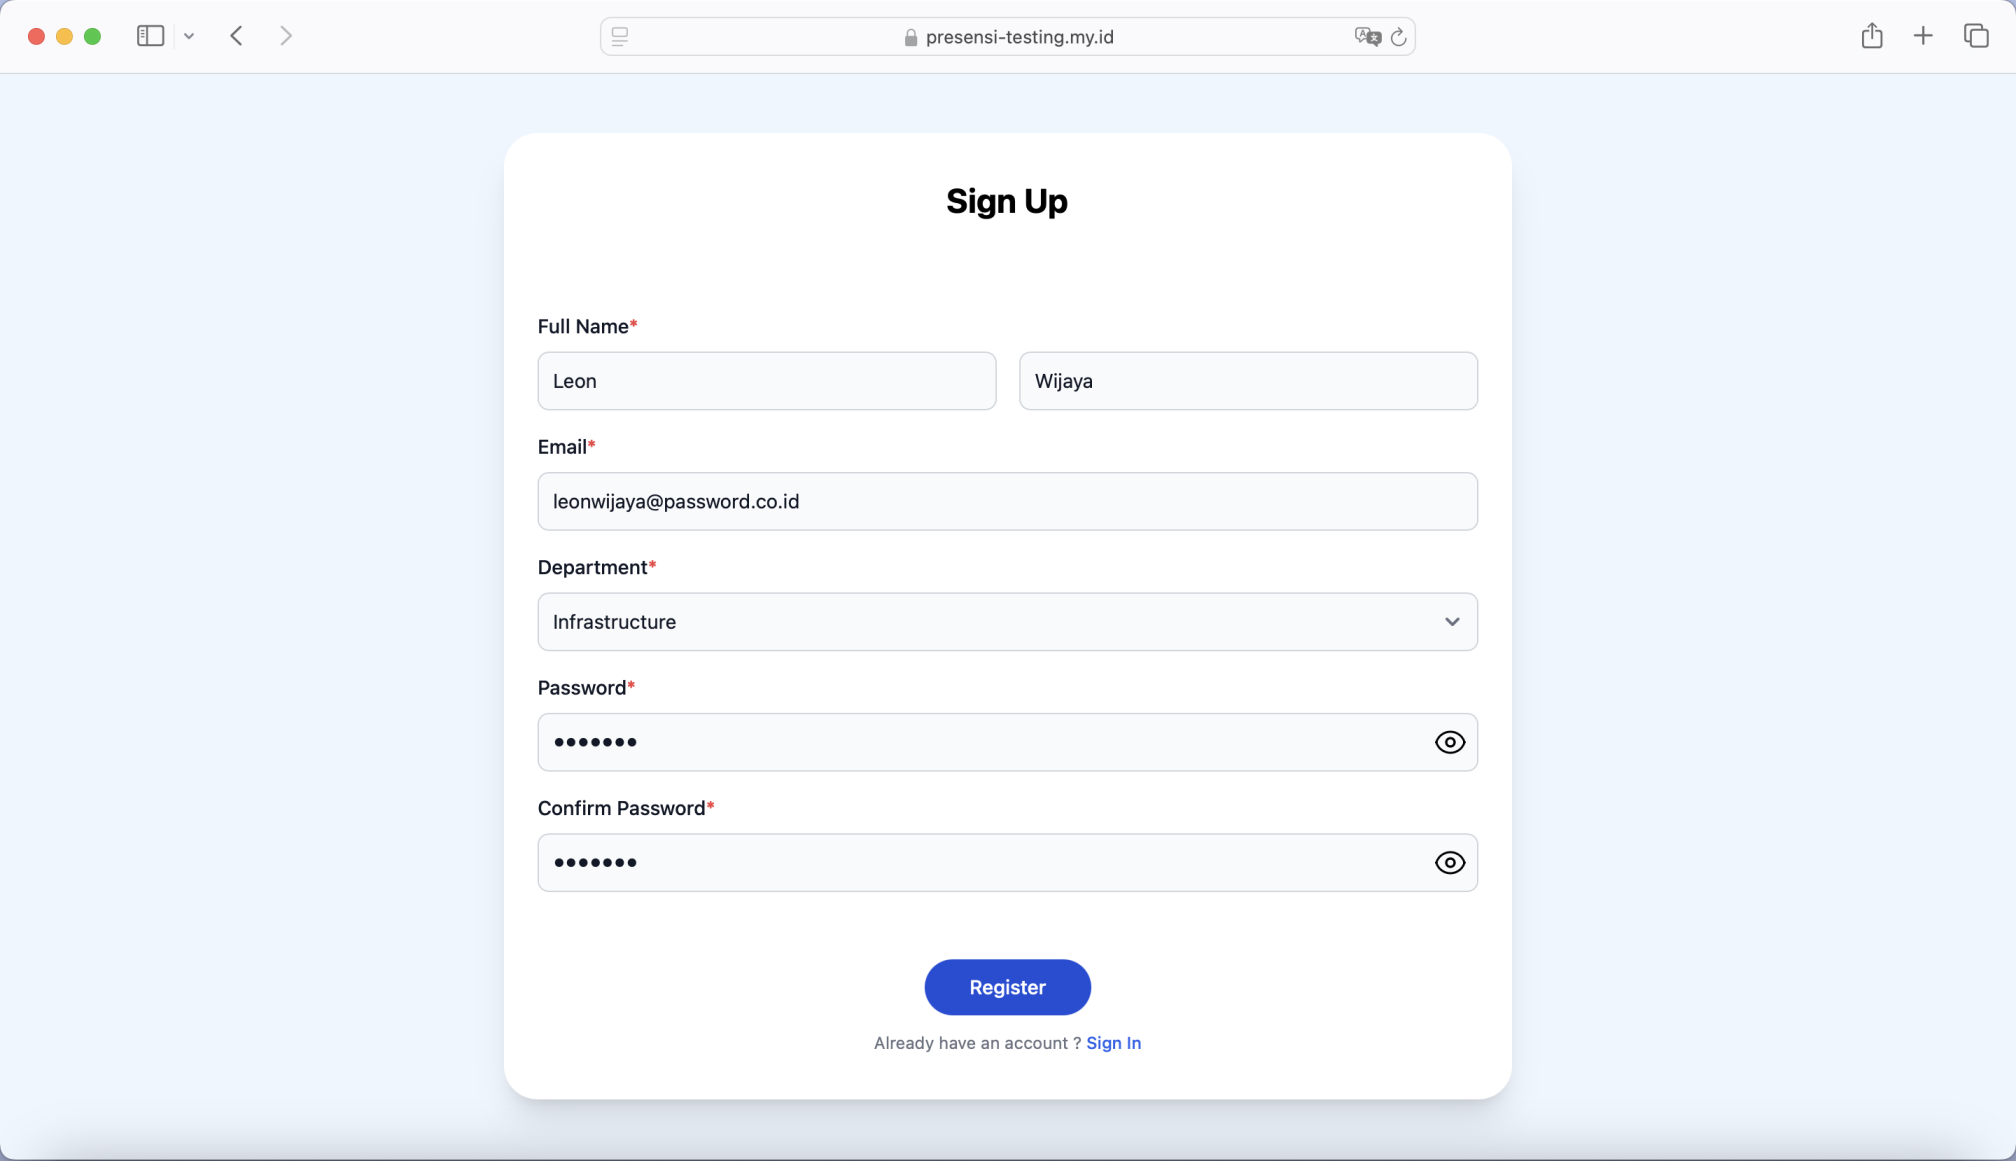
\includegraphics[width=10cm]{Gambar/bab3/user-manual/user-manual-halaman-sign-up.png}
    	\caption{Halaman Registrasi Akun}
    	\label{fig:user-manual-halaman-sign-up}
        \end{figure}
        \FloatBarrier

        \begin{figure}[!htbp]
    	\centering
    	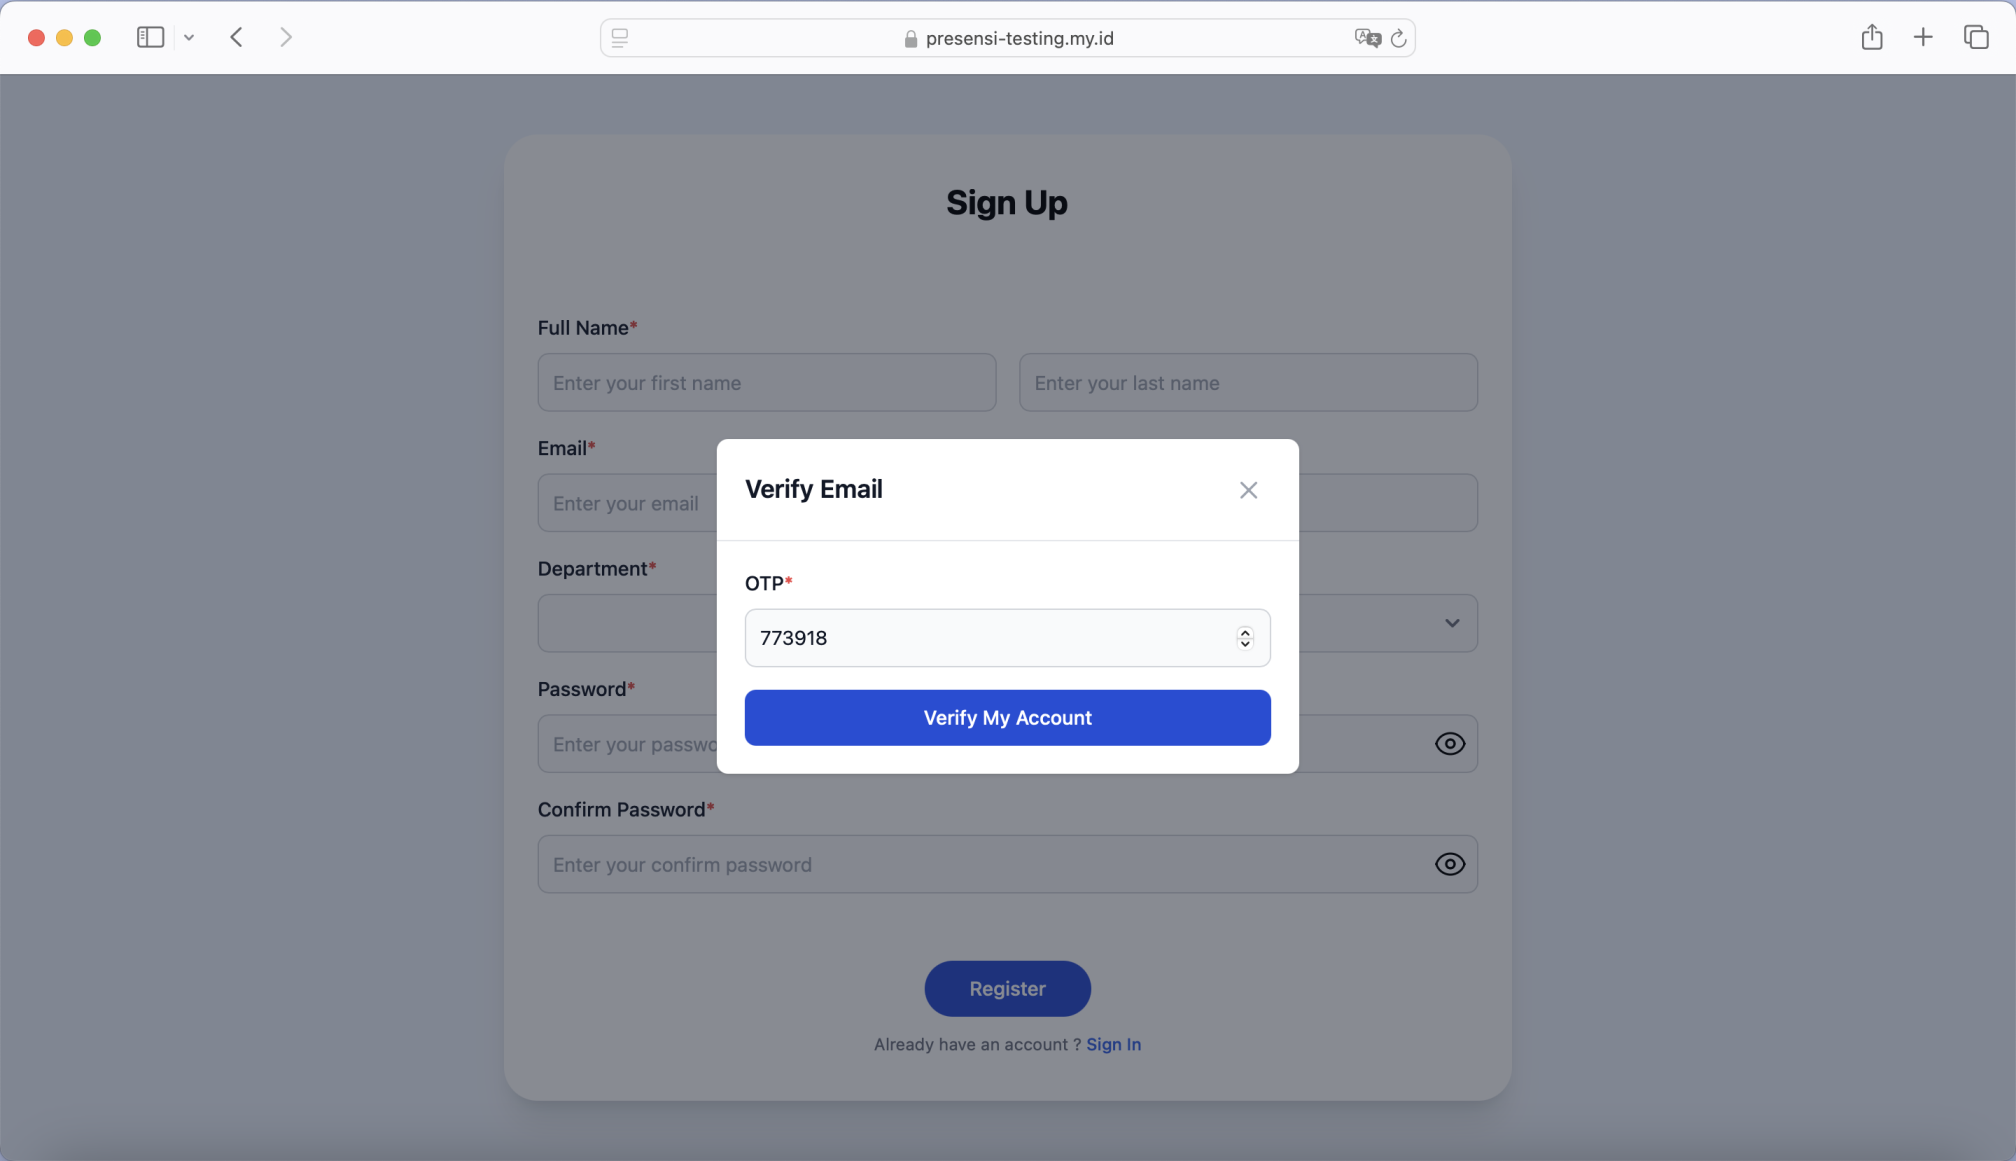
\includegraphics[width=10cm]{Gambar/bab3/user-manual/user-manual-verifikasi-email.png}
    	\caption{Modal Verifikasi \textit{Email}}
    	\label{fig:user-manual-verifikasi-email}
        \end{figure}
        \FloatBarrier

        \begin{figure}[!htbp]
    	\centering
    	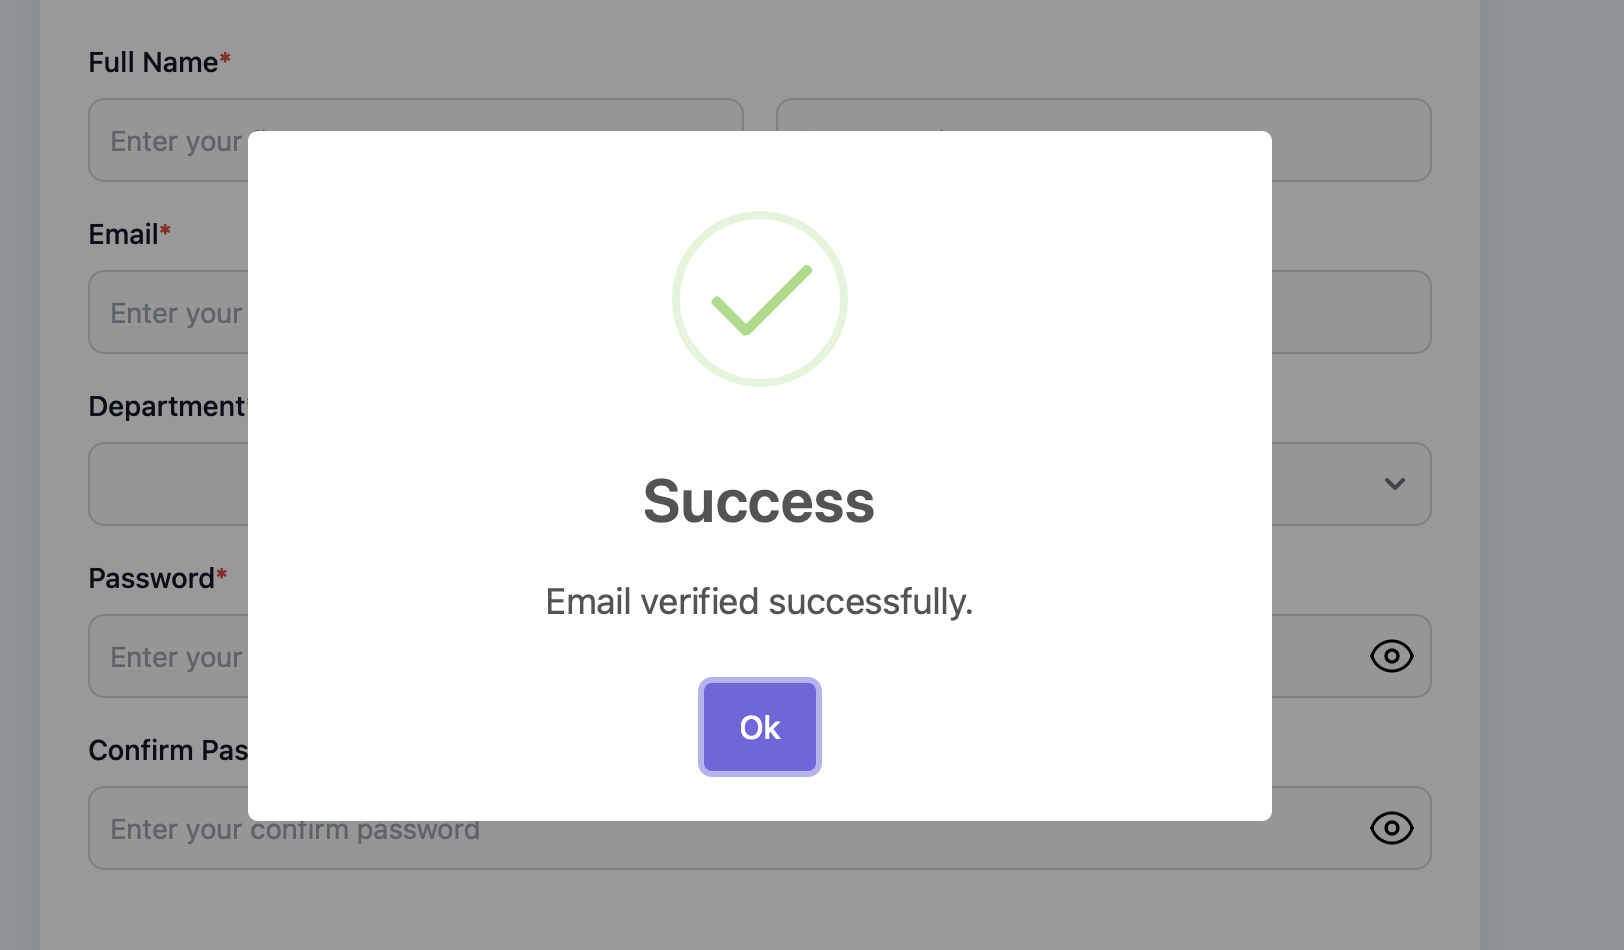
\includegraphics[width=10cm]{Gambar/bab3/user-manual/user-manual-berhasil-verifikasi.png}
    	\caption{Pesan Berhasil Verifikasi \textit{Email}}
    	\label{fig:user-manual-pesan-berhasil-verifikasi}
        \end{figure}
        \FloatBarrier
    \end{enumerate}

    \item Melihat Jadwal Kerja
    \begin{enumerate}
        \item Melakukan \textit{login} pada aplikasi presensi \textit{online} yang terdapat pada \textbf{Manual \ref{item:melakukan-login}}.
        \item Menekan tombol "\textit{Presence}" pada \textit{navigation bar} yang terletak di paling atas. \textbf{\ref{fig:user-manual-tombol-presence-pada-navigation-bar}} menunjukkan tombol \textit{"Presence"} pada \textit{navigation bar}.
        \item Pada halaman \textit{presence}, tekan tombol \textit{"Check Schedule"} yang terletak ditengah halaman. \textbf{\ref{fig:user-manual-tombol-check-schedule}} menunjukkan tombol \textit{"Check Schedule"} yang terletak di tengah halaman \textit{presence}.
        \item Tampilan modal informasi jadwal kerja akan muncul. \textbf{\ref{fig:user-manual-modal-check-schedule}} menunjukkan tampilan modal \textit{check schedule}.
        \begin{figure}[!htbp]
    	\centering
    	
\includegraphics[width=8cm]{Gambar/bab3/user-manual/user-manual-navbar-presence.png}
    	\caption{Tombol \textit{Presence} Pada \textit{Navigation Bar}}
    	\label{fig:user-manual-tombol-presence-pada-navigation-bar}
        \end{figure}
        \FloatBarrier
        \begin{figure}[!htbp]
    	\centering
    	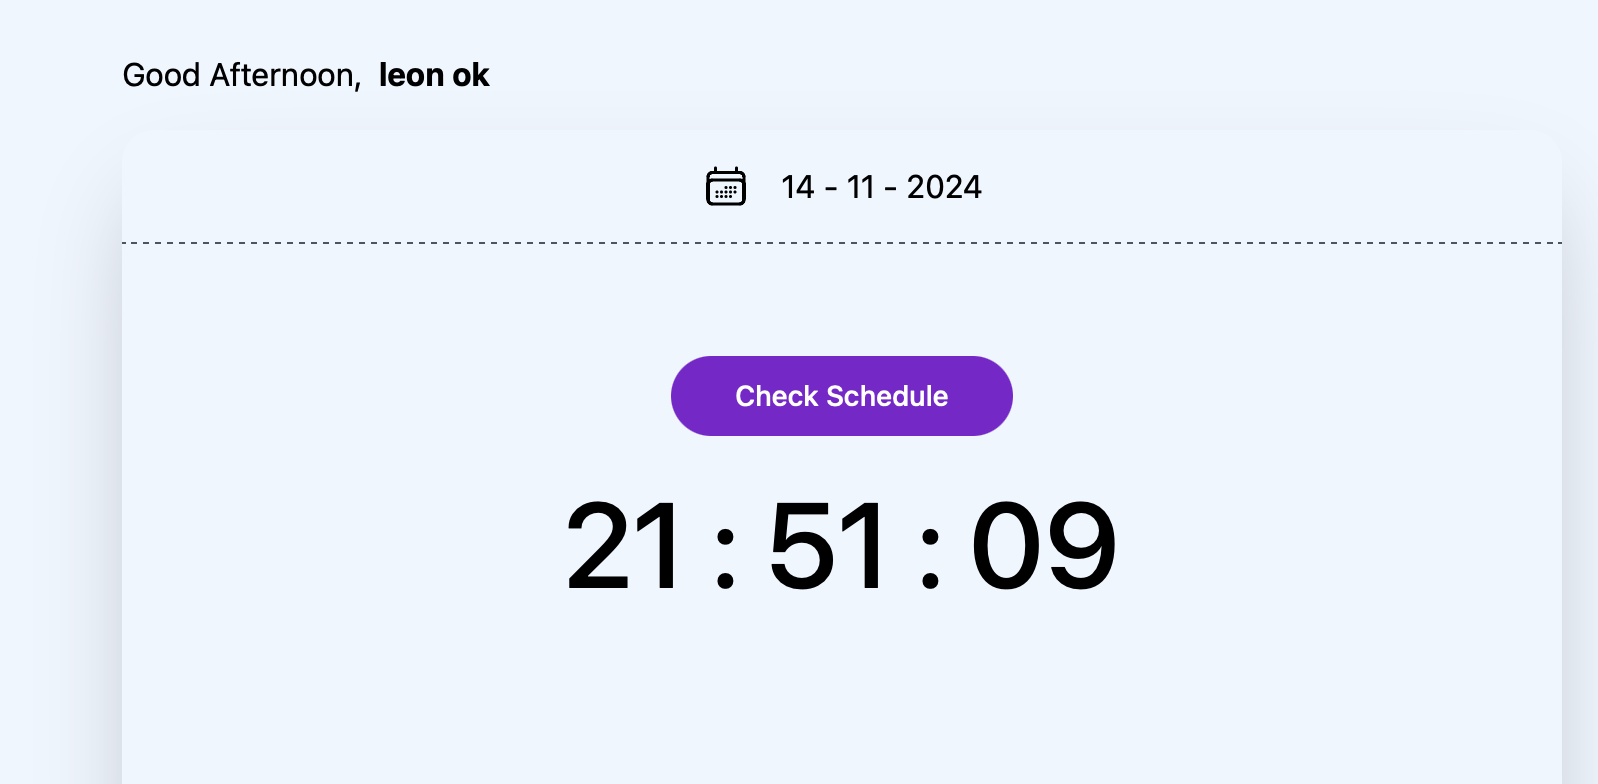
\includegraphics[width=8cm]{Gambar/bab3/user-manual/user-manual-tombol-check-schedule.png}
    	\caption{Tombol \textit{Check Schedule} Pada Halaman \textit{Presence}}
    	\label{fig:user-manual-tombol-check-schedule}
        \end{figure}
        \FloatBarrier
        \begin{figure}[!htbp]
    	\centering
    	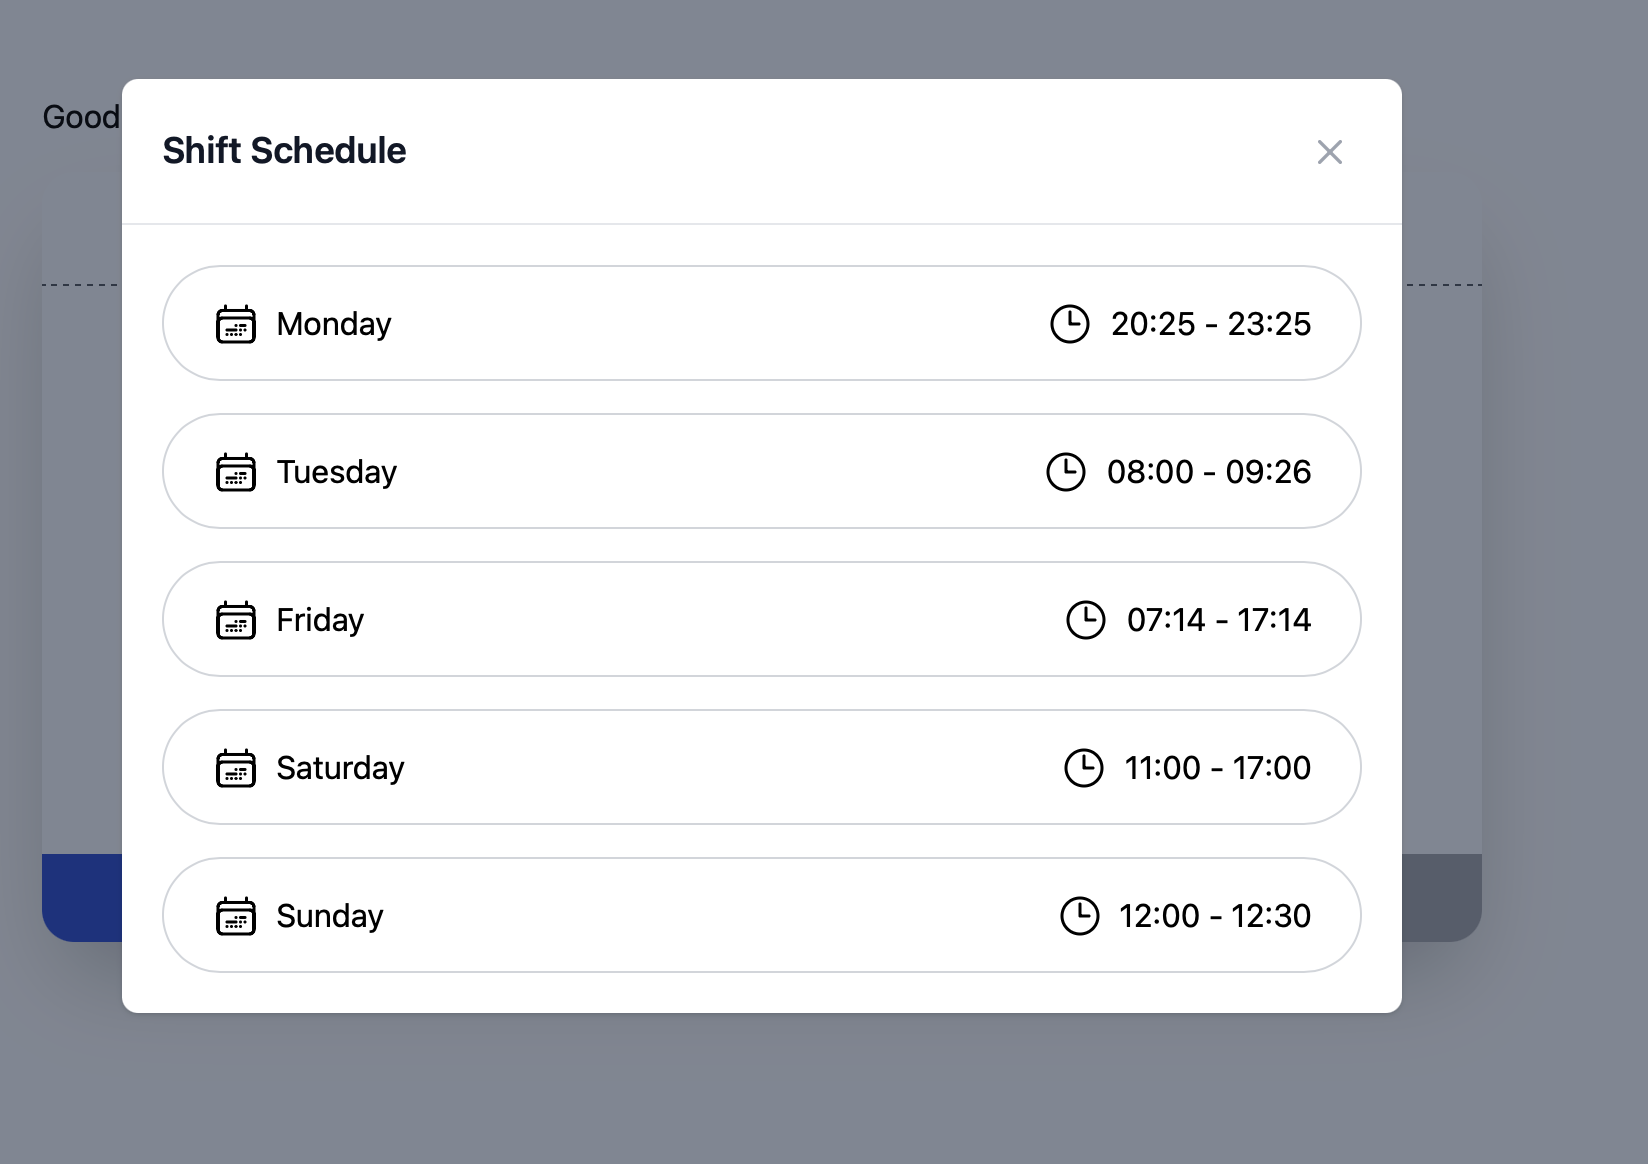
\includegraphics[width=8cm]{Gambar/bab3/user-manual/user-manual-modal-check-schedule.png}
    	\caption{Tampilan Modal \textit{Check Schedule}}
    	\label{fig:user-manual-modal-check-schedule}
        \end{figure}
        \FloatBarrier
    \end{enumerate}

    \item Melakukan \textit{Clock In}
    \begin{enumerate}
        \item Melakukan \textit{login} pada aplikasi presensi \textit{online} yang terdapat pada \textbf{Manual \ref{item:melakukan-login}}.
        \item Menekan tombol "\textit{Presence}" pada \textit{navigation bar} yang terletak di paling atas. \textbf{\ref{fig:user-manual-tombol-presence-pada-navigation-bar}} menunjukkan tombol \textit{"Presence"} pada \textit{navigation bar}.
        \item Pada halaman \textit{presence}, tekan tombol \textit{"Clock In"} yang berada ditengah halaman dan izinkan perangkat untuk mengakses lokasi. \textbf{\ref{fig:user-manual-tombol-clock-in}} menunjukkan tombol "\textit{Clock In}" pada halaman \textit{presence}.
        \begin{figure}[!htbp]
    	\centering
    	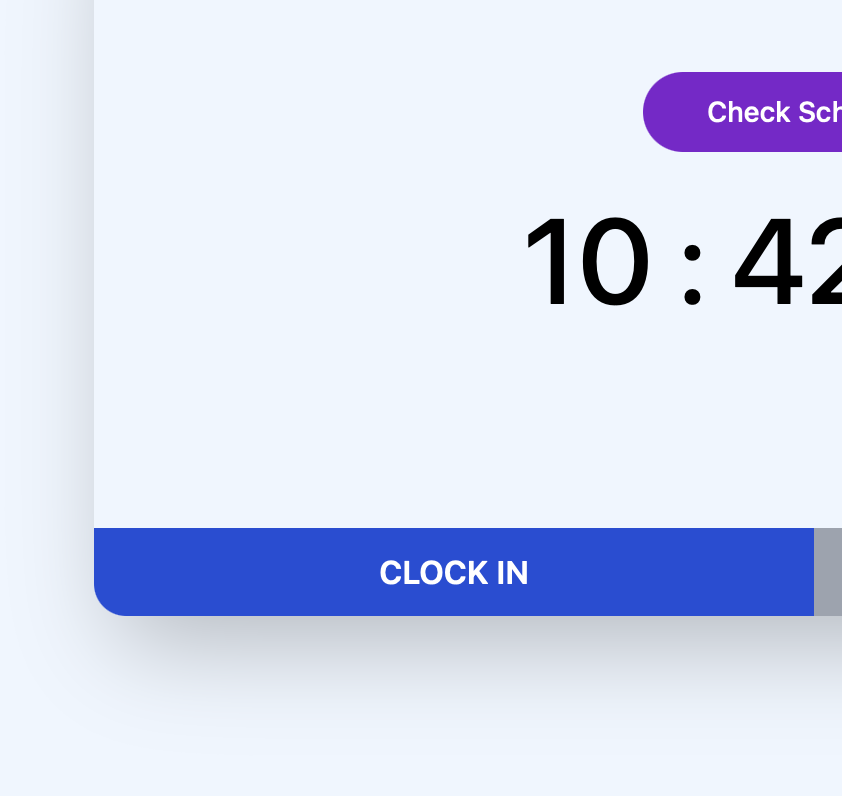
\includegraphics[width=8cm]{Gambar/bab3/user-manual/user-manual-tombol-clock-in.png}
    	\caption{Tombol \textit{Clock In} Pada Halaman \textit{Presence}}
    	\label{fig:user-manual-tombol-clock-in}
        \end{figure}
        \FloatBarrier
        \item Mengisi seluruh \textit{input form} pada modal \textit{clock in}. \textbf{\ref{fig:user-manual-modal-clock-in}} menunjukkan tampilan modal \textit{clock in}.
        \begin{figure}[!htbp]
    	\centering
    	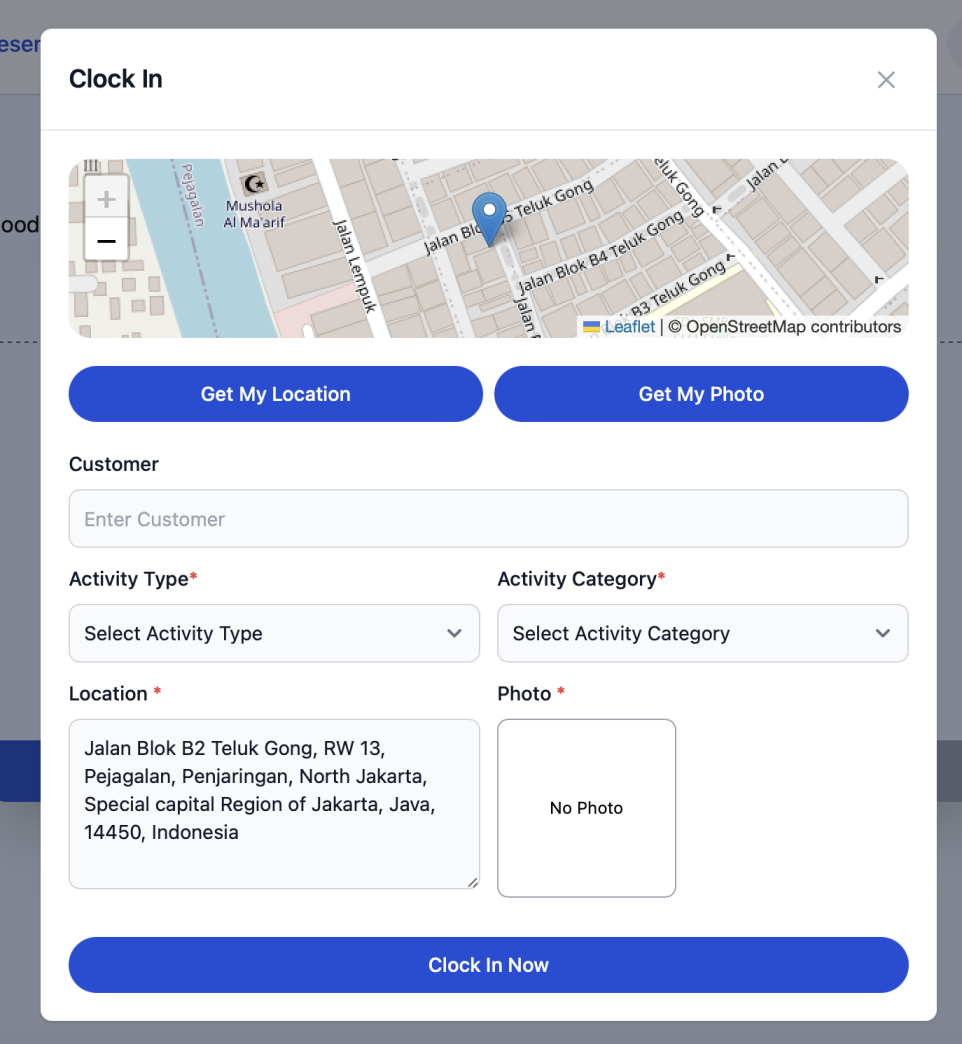
\includegraphics[width=5cm]{Gambar/bab3/user-manual/user-manual-modal-clock-in.png}
    	\caption{Modal \textit{Clock In}}
    	\label{fig:user-manual-modal-clock-in}
        \end{figure}
        \FloatBarrier
        \item Menekan tombol "\textit{Get My Photo}" pada modal \textit{clock in} untuk mengambil foto presensi dan izinkan perangkat untuk mengakses kamera. \textbf{\ref{fig:user-manual-tombol-get-my-photo-pada-modal-clock-in}} menunjukkan tombol "\textit{Get My Photo}" pada modal \textit{clock in}.
        \begin{figure}[!htbp]
    	\centering
    	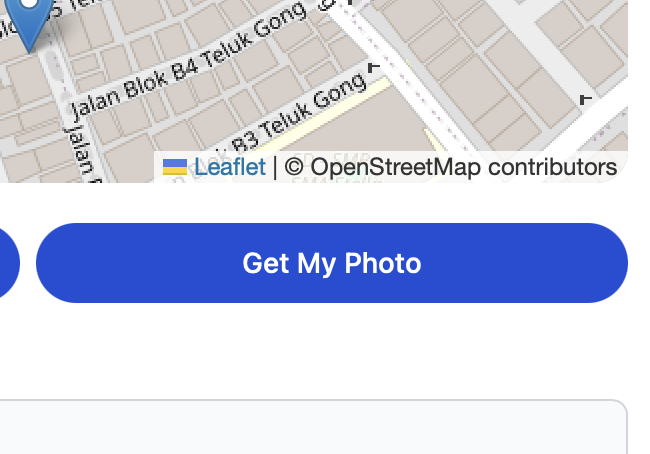
\includegraphics[width=8cm]{Gambar/bab3/user-manual/user-manual-tombol-get-my-photo-clock-in.png}
    	\caption{Tombol \textit{Get My Photo} Pada Modal \textit{Clock In}}
    	\label{fig:user-manual-tombol-get-my-photo-pada-modal-clock-in}
        \end{figure}
        \FloatBarrier

        \item Mengambil foto wajah pada modal kamera, pastikan posisi kepala berada ditengah lingkaran yang telah ditentukan pada kamera dan tekan tombol bulat untuk mengambil foto. \textbf{\ref{fig:user-manual-modal-kamera-clock-in}} menunjukkan tampilan modal kamera saat \textit{clock in}.
        \begin{figure}[!htbp]
    	\centering
    	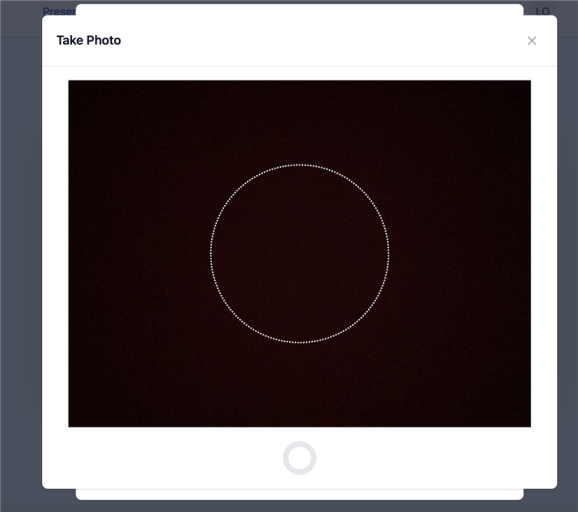
\includegraphics[width=8cm]{Gambar/bab3/user-manual/user-manual-modal-kamera-clock-in.png}
    	\caption{Modal Kamera \textit{Clock In}}
    	\label{fig:user-manual-modal-kamera-clock-in}
        \end{figure}
        \FloatBarrier
        \item Saat berhasil ambil foto, maka modal kamera akan tertutup dan membuka modal \textit{clock in} kembali. Tekan tombol \textit{"Clock In Now"} untuk menyimpan presensi masuk. \textbf{\ref{fig:user-manual-tombol-clock-in-now-pada-modal-clock-in}} menunjukkan tombol "\textit{Clock In Now}" pada modal \textit{clock in}.
        \begin{figure}[!htbp]
    	\centering
    	
\includegraphics[width=8cm]{Gambar/bab3/user-manual/user-manual-tombol-clock-in-now.png}
    	\caption{Tombol \textit{Clock In Now} Pada Modal \textit{Clock In}}
    	\label{fig:user-manual-tombol-clock-in-now-pada-modal-clock-in}
        \end{figure}
        \FloatBarrier
    \end{enumerate}

    \item Melakukan \textit{Clock Out}
    \begin{enumerate}
        \item Melakukan \textit{login} pada aplikasi presensi \textit{online} yang terdapat pada \textbf{Manual \ref{item:melakukan-login}}.
        \item Menekan tombol "\textit{Presence}" pada \textit{navigation bar} yang terletak di paling atas. \textbf{\ref{fig:user-manual-tombol-presence-pada-navigation-bar}} menunjukkan tombol \textit{"Presence"} pada \textit{navigation bar}.
        \item Pastikan sudah melakukan \textit{clock in} sebelumya, pada halaman \textit{presence}, tekan tombol \textit{"Clock Out"} yang berada ditengah halaman dan izinkan perangkat untuk mengakses lokasi. \textbf{\ref{fig:user-manual-tombol-clock-out}} menunjukkan tombol "\textit{Clock Out}" pada halaman \textit{presence}.
        \begin{figure}[!htbp]
    	\centering
    	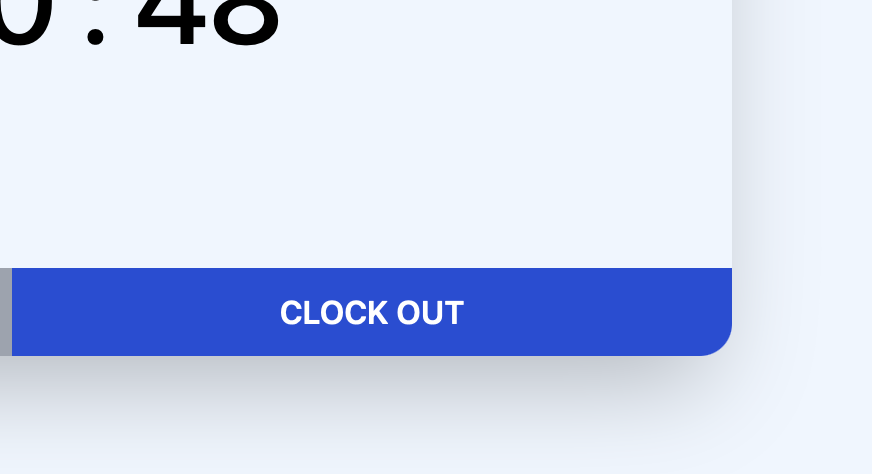
\includegraphics[width=8cm]{Gambar/bab3/user-manual/user-manual-tombol-clock-out.png}
    	\caption{Tombol \textit{Clock Out} Pada Halaman \textit{Presence}}
    	\label{fig:user-manual-tombol-clock-out}
        \end{figure}
        \FloatBarrier
        \item Seluruh \textit{input form} pada modal \textit{clock out} dapat dilakukan perubahan. \textbf{\ref{fig:user-manual-modal-clock-out}} menunjukkan tampilan modal \textit{clock out}.
        \begin{figure}[!htbp]
    	\centering
    	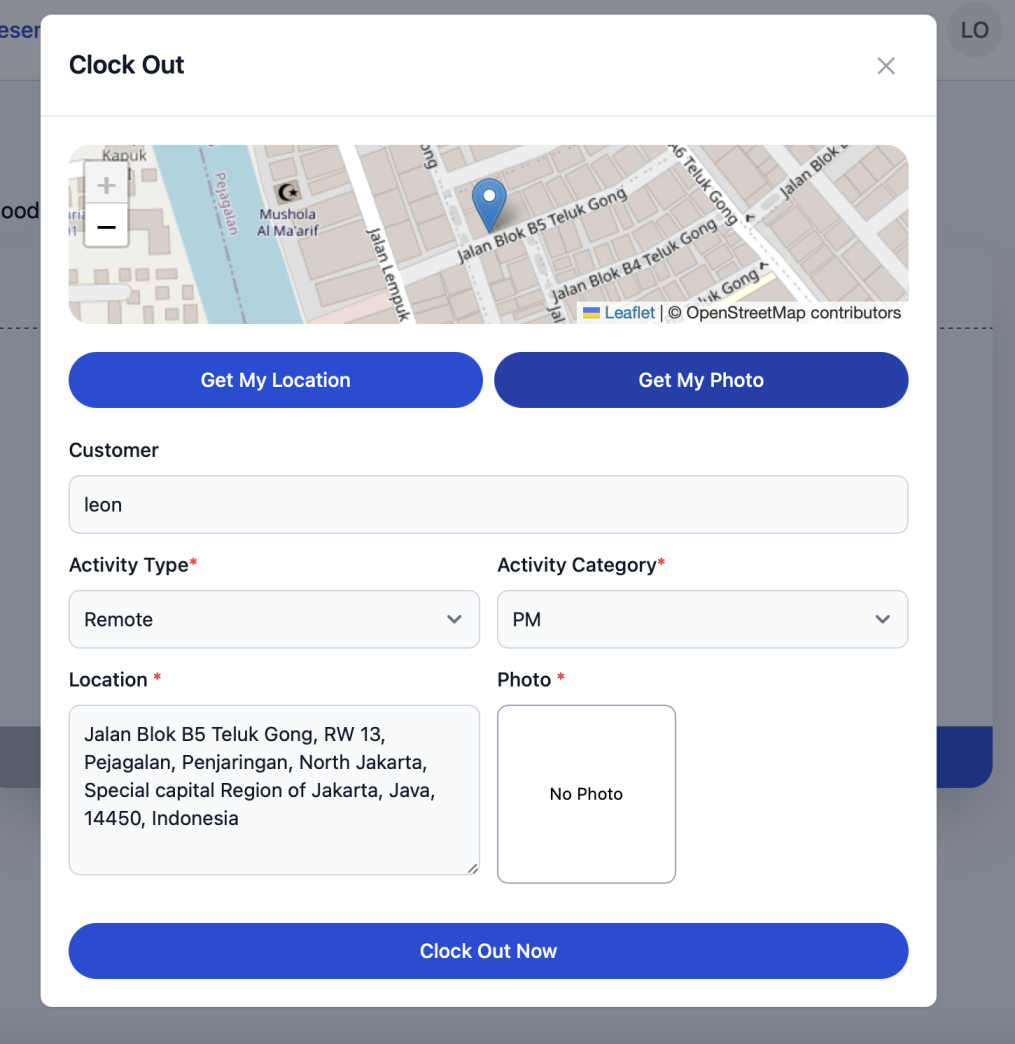
\includegraphics[width=5cm]{Gambar/bab3/user-manual/user-manual-modal-clock-out.png}
    	\caption{Modal \textit{Clock Out}}
    	\label{fig:user-manual-modal-clock-out}
        \end{figure}
        \FloatBarrier
        \item Menekan tombol "\textit{Get My Photo}" pada modal \textit{clock out} untuk mengambil foto presensi dan izinkan perangkat untuk mengakses kamera. \textbf{\ref{fig:user-manual-tombol-get-my-photo-pada-modal-clock-out}} menunjukkan tombol "\textit{Get My Photo}" pada modal \textit{clock out}.
        \begin{figure}[!htbp]
    	\centering
    	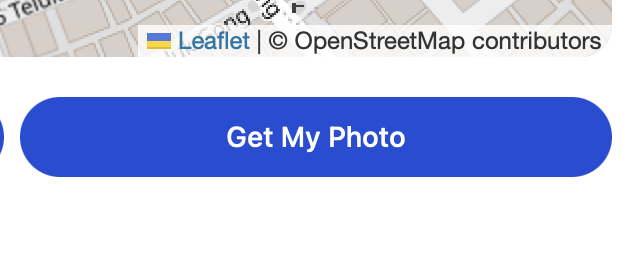
\includegraphics[width=8cm]{Gambar/bab3/user-manual/user-manual-get-my-photo-clock-out.png}
    	\caption{Tombol \textit{Get My Photo} Pada Modal \textit{Clock Out}}
    	\label{fig:user-manual-tombol-get-my-photo-pada-modal-clock-out}
        \end{figure}
        \FloatBarrier

        \item Mengambil foto wajah pada modal kamera, pastikan posisi kepala berada ditengah lingkaran yang telah ditentukan pada kamera dan tekan tombol bulat untuk mengambil foto. \textbf{\ref{fig:user-manual-modal-kamera-clock-out}} menunjukkan tampilan modal kamera saat \textit{clock out}.
        \begin{figure}[!htbp]
    	\centering
    	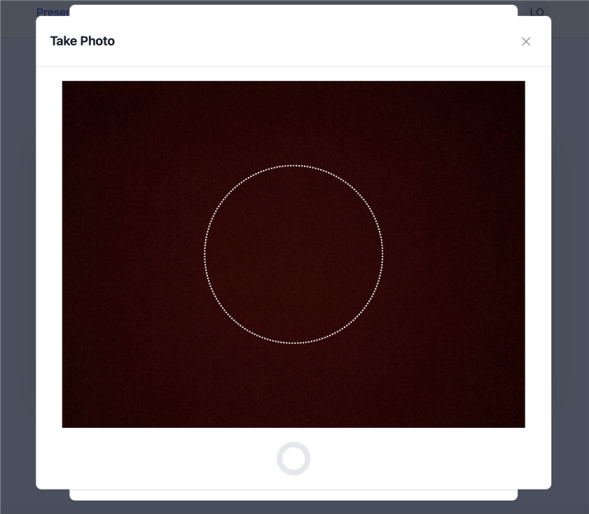
\includegraphics[width=8cm]{Gambar/bab3/user-manual/user-manual-modal-kamera-clock-out.png}
    	\caption{Modal Kamera \textit{Clock Out}}
    	\label{fig:user-manual-modal-kamera-clock-out}
        \end{figure}
        \FloatBarrier
        \item Saat berhasil ambil foto, maka modal kamera akan tertutup dan membuka modal \textit{clock out} kembali. Tekan tombol \textit{"Clock Out Now"} untuk menyimpan presensi keluar. \textbf{\ref{fig:user-manual-tombol-clock-out-now-pada-modal-clock-out}} menunjukkan tombol "\textit{Clock Out Now}" pada modal \textit{clock in}.
        \begin{figure}[!htbp]
    	\centering
    	
\includegraphics[width=8cm]{Gambar/bab3/user-manual/user-manual-tombol-clock-out-now.png}
    	\caption{Tombol \textit{Clock Out Now} Pada Modal \textit{Clock Out}}
    	\label{fig:user-manual-tombol-clock-out-now-pada-modal-clock-out}
        \end{figure}
        \FloatBarrier
    \end{enumerate}

    \item Melakukan Pengajuan Lembur Manual
    \begin{enumerate}
        \item Melakukan \textit{login} pada aplikasi presensi \textit{online} yang terdapat pada \textbf{Manual \ref{item:melakukan-login}}.
        \item Menekan tombol "\textit{Request}" pada \textit{navigation bar} yang terletak di paling atas. \textbf{\ref{fig:user-manual-tombol-request-pada-navigation-bar}} menunjukkan tombol \textit{"Request"} pada \textit{navigation bar}.
        \begin{figure}[!htbp]
    	\centering
    	
\includegraphics[width=8cm]{Gambar/bab3/user-manual/user-manual-navbar-request.png}
    	\caption{Tombol \textit{Request} Pada \textit{Navigation Bar}}
    	\label{fig:user-manual-tombol-request-pada-navigation-bar}
        \end{figure}
        \FloatBarrier
        \item Mengisi seluruh \textit{input form} pada halaman \textit{request} dan tekan tombol \textit{"Submit"} untuk menyimpan data pengajuan lembur. \textbf{\ref{fig:user-manual-halaman-pengajuan-lembur-manual}} menunjukkan halaman pengajuan lembur manual.
        \begin{figure}[!htbp]
    	\centering
    	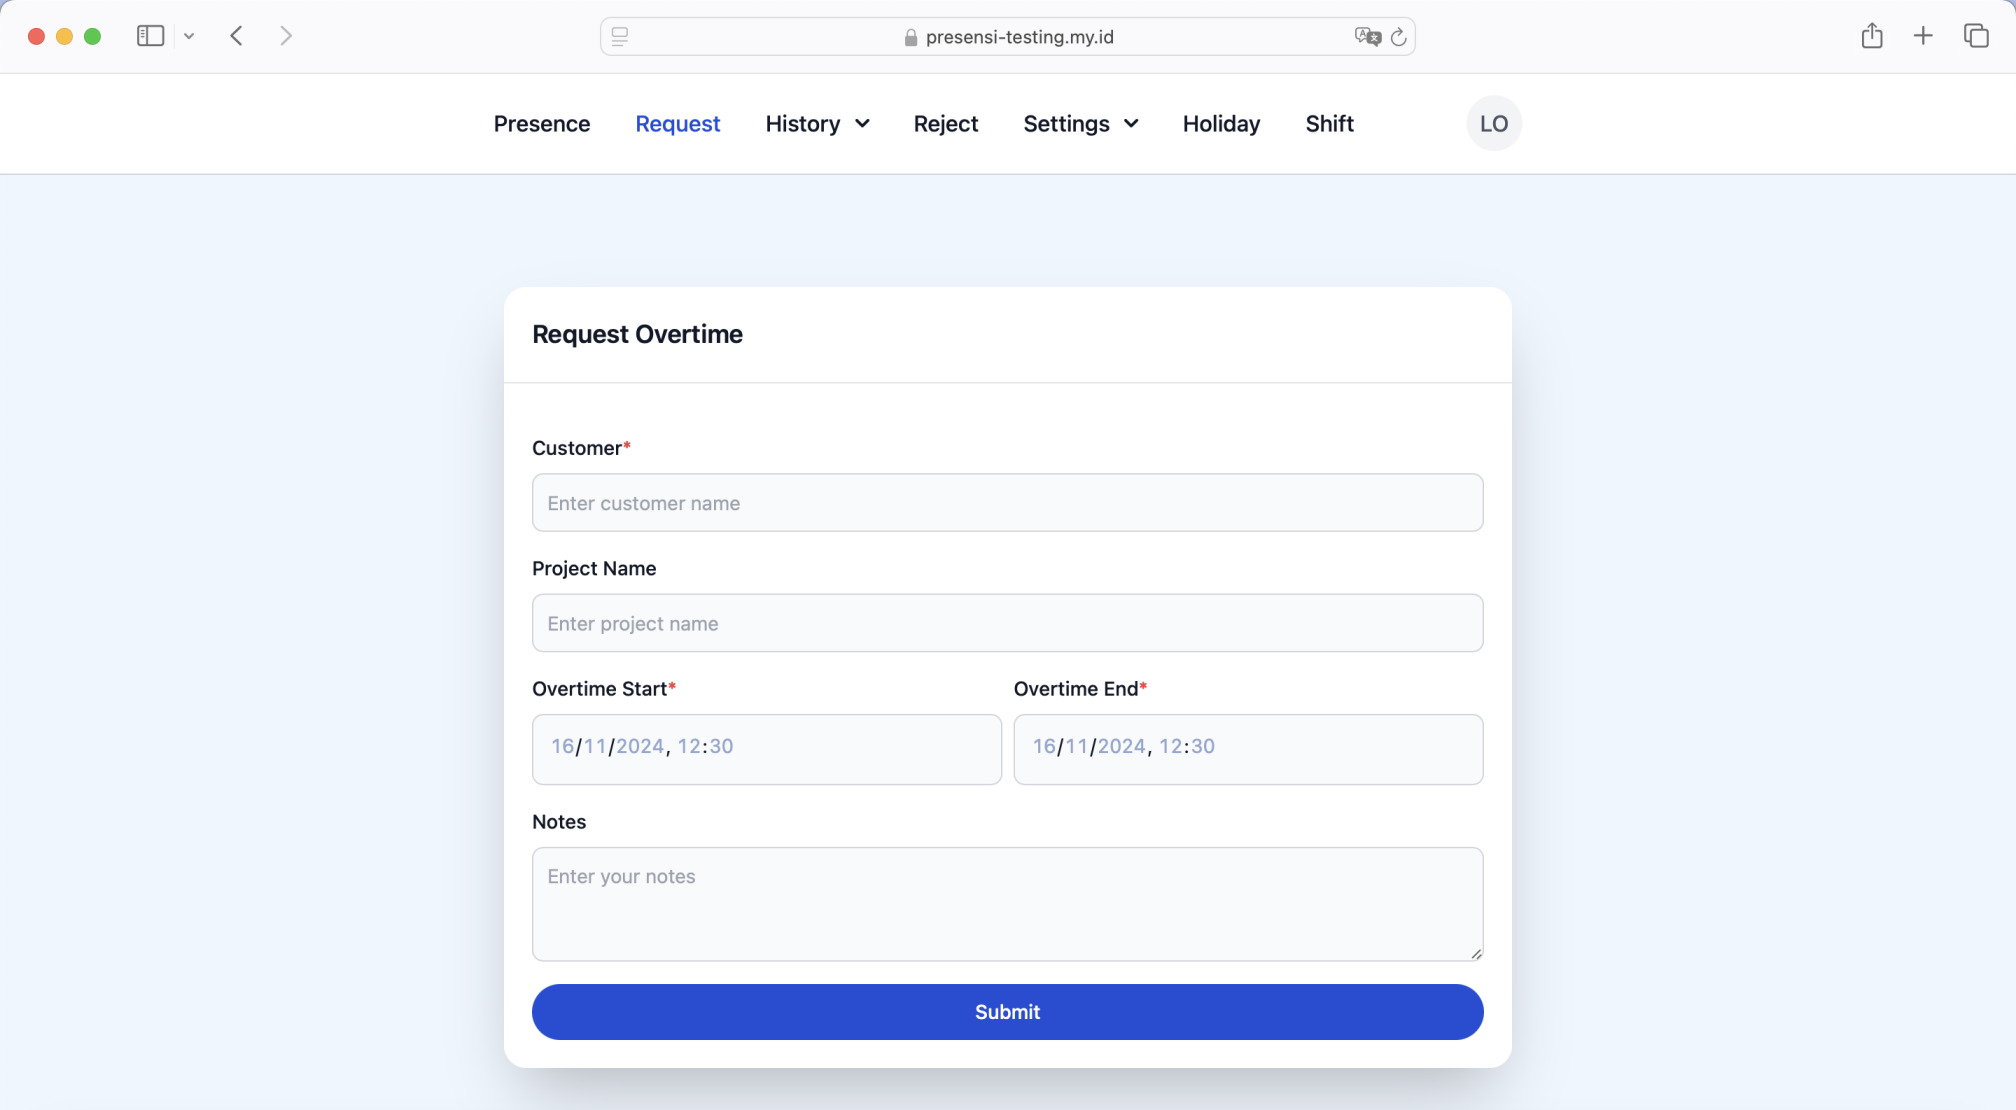
\includegraphics[width=8cm]{Gambar/bab3/user-manual/user-manual-pengajuan-lembur-manual.png}
    	\caption{Tampilan Halaman Pengajuan Lembur Manual}
    	\label{fig:user-manual-halaman-pengajuan-lembur-manual}
        \end{figure}
        \FloatBarrier
    \end{enumerate}

    \item Melihat Riwayat Presensi\label{item:melihat-riwayat-presensi}
    \begin{enumerate}
        \item Melakukan \textit{login} pada aplikasi presensi \textit{online} yang terdapat pada \textbf{Manual \ref{item:melakukan-login}}.
        \item Menekan tombol "\textit{History}" pada \textit{navigation bar} yang terletak di paling atas dan memilih tombol \textit{"Attendance History"}. \textbf{\ref{fig:user-manual-tombol-attendance-history-pada-navigation-bar}} menunjukkan tombol \textit{"Attendance History"} pada \textit{navigation bar}.
        \begin{figure}[!htbp]
    	\centering
    	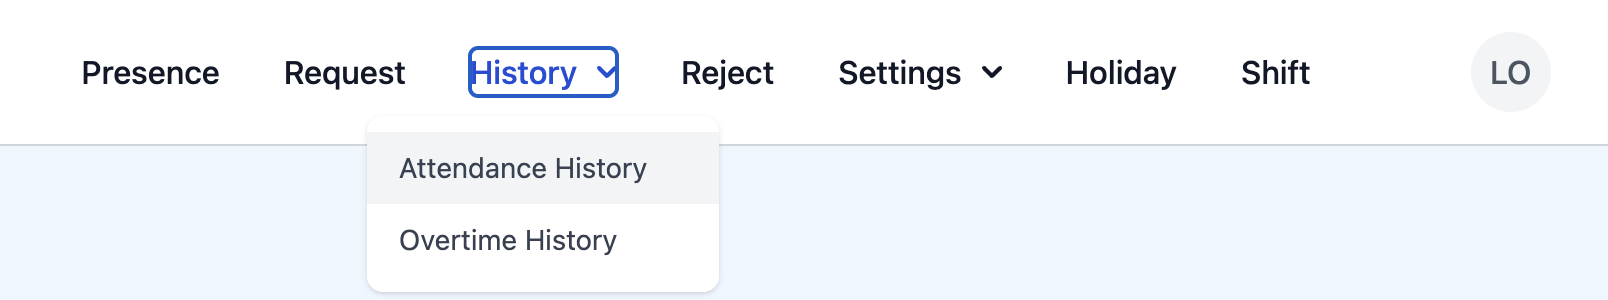
\includegraphics[width=8cm]{Gambar/bab3/user-manual/user-manual-navbar-attendance-history.png}
    	\caption{Tombol \textit{Attendance History} Pada \textit{Navigation Bar}}
    	\label{fig:user-manual-tombol-attendance-history-pada-navigation-bar}
        \end{figure}
        \FloatBarrier
        \item Seluruh daftar data riwayat presensi akan ditampilkan pada halaman \textit{attendance history}. \textbf{\ref{fig:user-manual-halaman-riwayat-presensi}} menunjukkan halaman \textit{attendance history}. 
        \begin{figure}[!htbp]
    	\centering
    	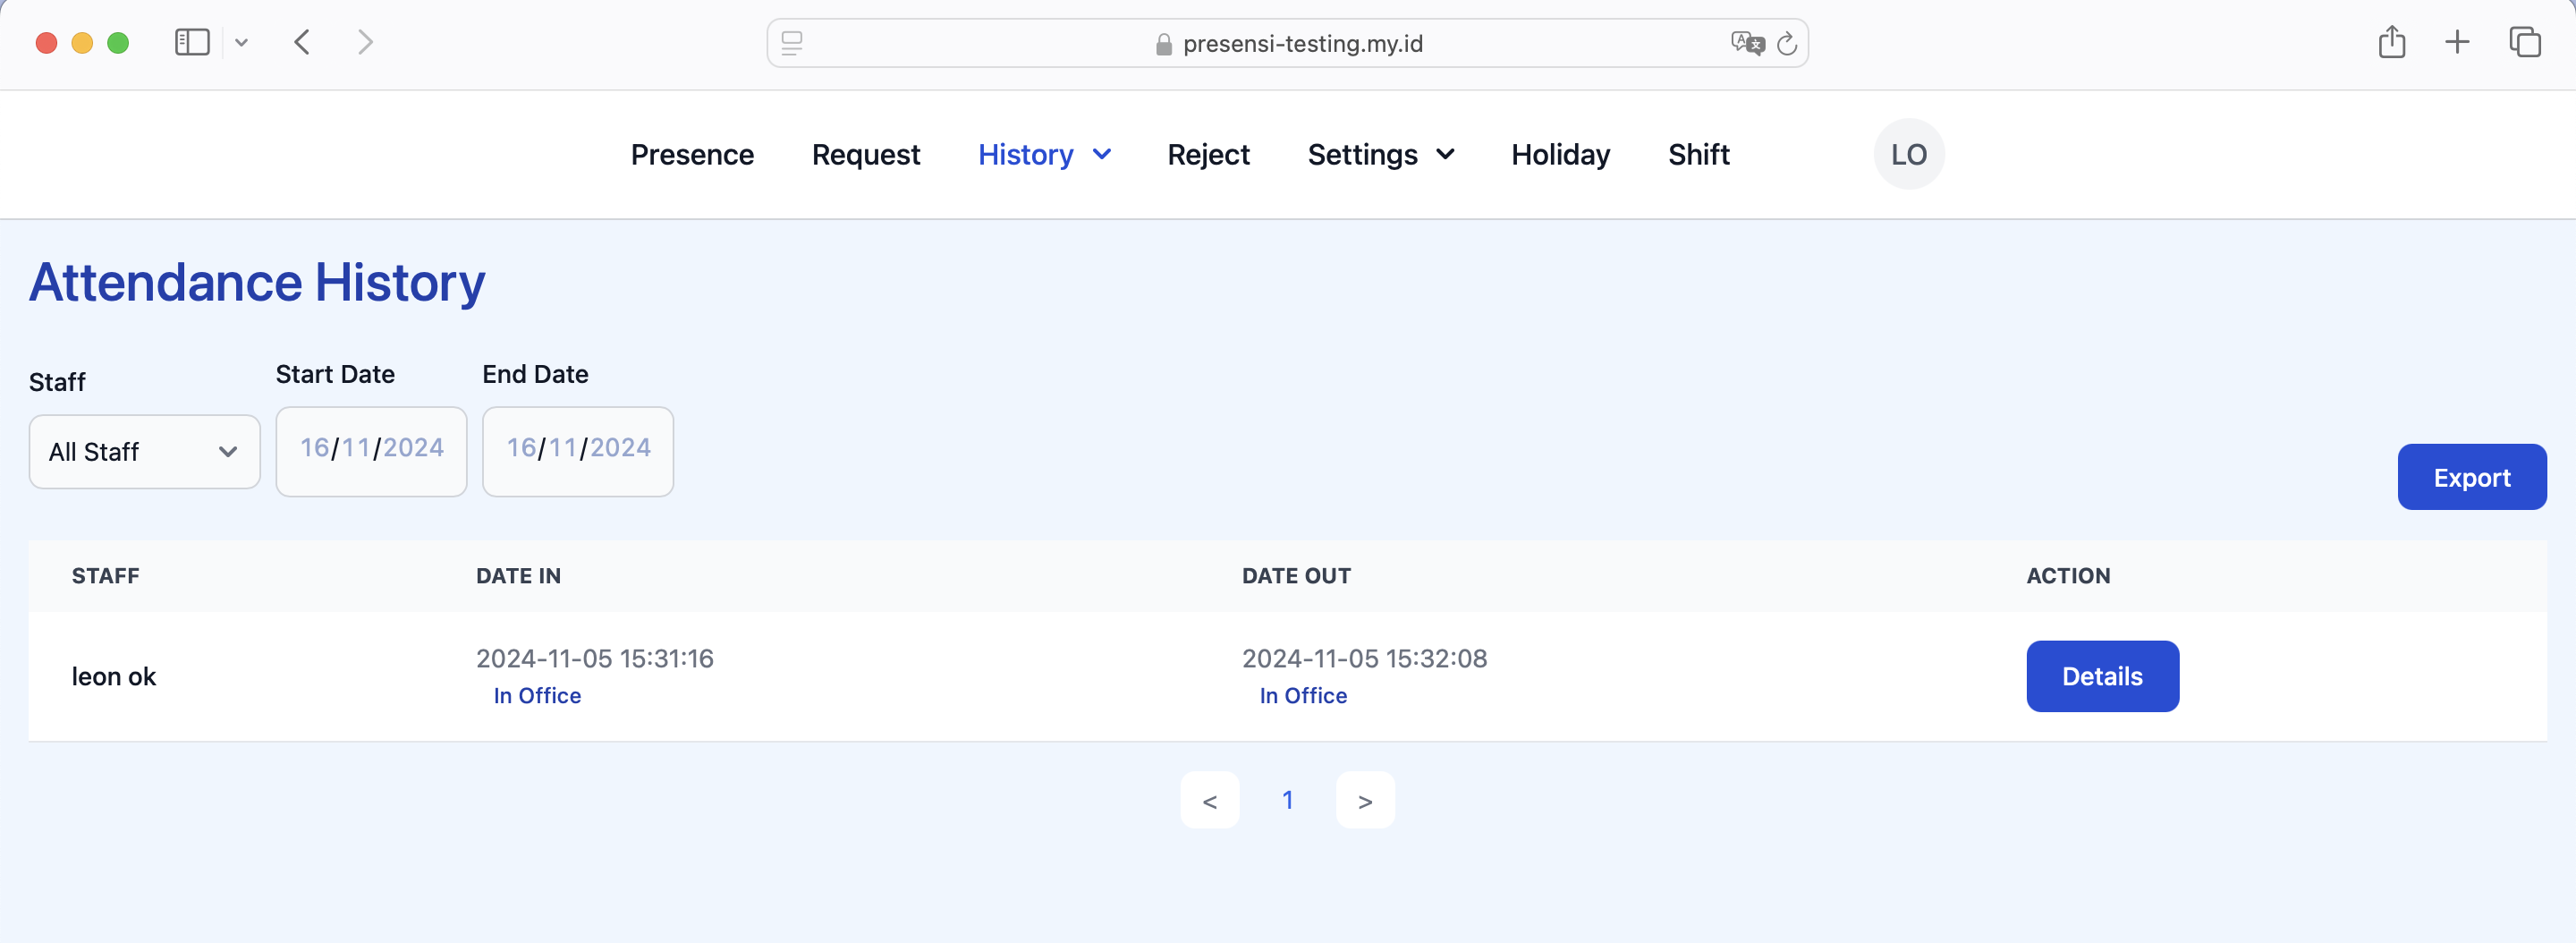
\includegraphics[width=8cm]{Gambar/bab3/user-manual/user-manual-halaman-riwayat-presensi.png}
    	\caption{Halaman \textit{Attendance History}}
    	\label{fig:user-manual-halaman-riwayat-presensi}
        \end{figure}
        \FloatBarrier
    \end{enumerate}

    \item Melihat Detail Riwayat Presensi
    \begin{enumerate}
        \item Membuka halaman riwayat presensi yang terdapat pada \textbf{Manual \ref{item:melihat-riwayat-presensi}}.
        \item Menekan tombol "\textit{Detail}" pada salah satu data presensi. Sistem akan menampilkan modal detail riwayat presensi beserta informasi lengkap riwayat presensi. \textbf{\ref{fig:user-manual-modal-attendance-history-details}} menunjukkan modal \textit{attendance history details}.
        \begin{figure}[!htbp]
    	\centering
    	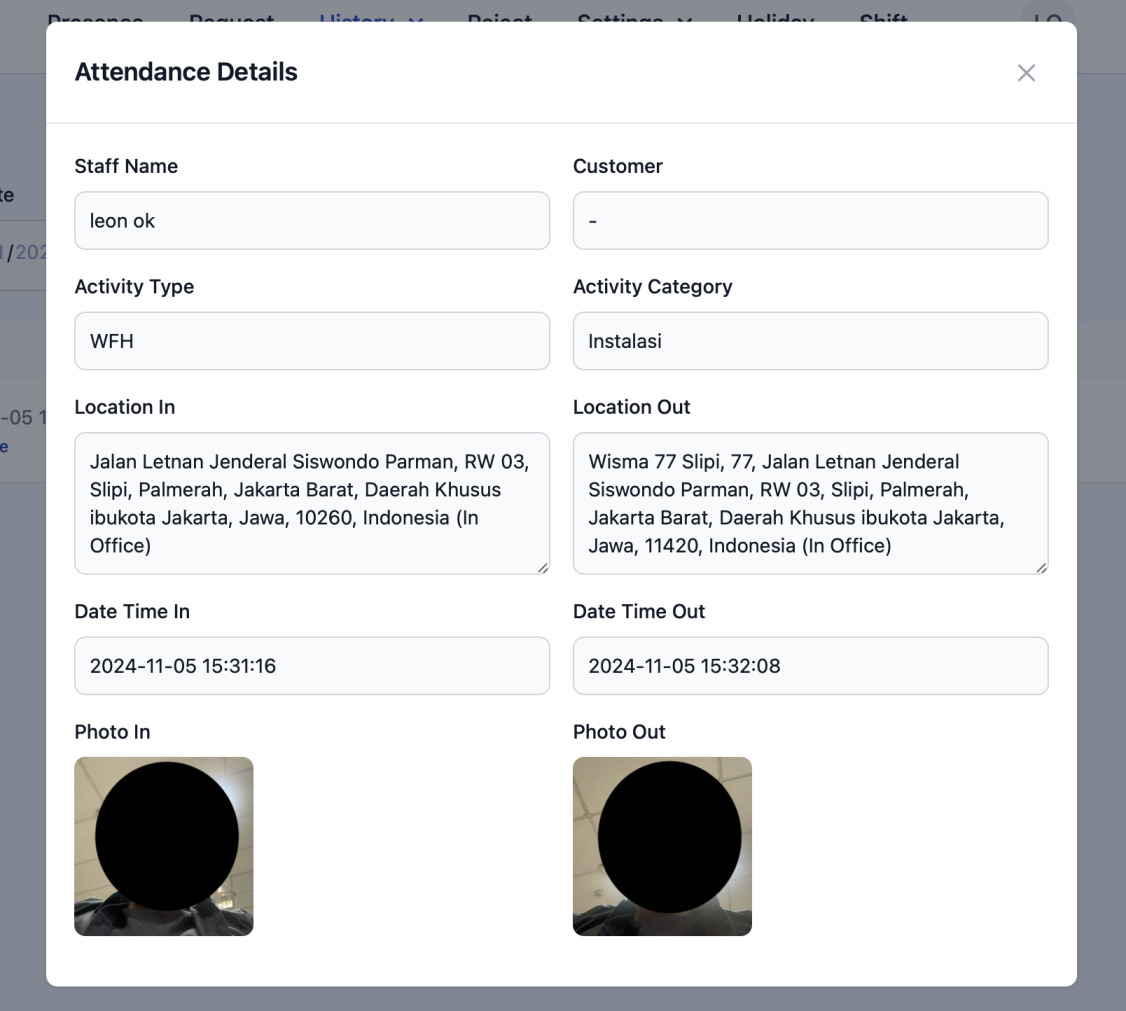
\includegraphics[width=8cm]{Gambar/bab3/user-manual/user-manual-detail-riwayat-presensi.png}
    	\caption{Modal \textit{Attendance History Details}}
    	\label{fig:user-manual-modal-attendance-history-details}
        \end{figure}
        \FloatBarrier
    \end{enumerate}

    \item Melakukan \textit{Export} Data Riwayat Presensi
    \begin{enumerate}
        \item Membuka halaman riwayat presensi yang terdapat pada \textbf{Manual \ref{item:melihat-riwayat-presensi}}.
        \item Menekan tombol \textit{"Export"} yang terdapat pada halaman riwayat presensi. \textbf{\ref{fig:user-manual-tombol-export-riwayat-presensi}} menunjukkan tombol untuk \textit{export} riwayat presensi menjadi format \textit{Excel}.
        \begin{figure}[!htbp]
    	\centering
    	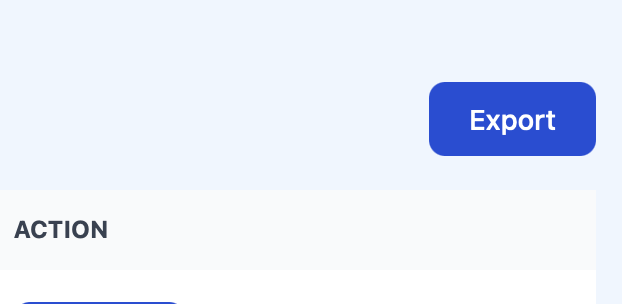
\includegraphics[width=8cm]{Gambar/bab3/user-manual/user-manual-tombol-export-riwayat-presensi.png}
    	\caption{Tombol \textit{Export} Riwayat Presensi}
    	\label{fig:user-manual-tombol-export-riwayat-presensi}
        \end{figure}
        \FloatBarrier
        \item Perangkat akan otomatis men-\textit{download file Excel} yang berisi data presensi. \textbf{\ref{fig:user-manual-file-excel-riwayat-presensi}} menunjukkan \textit{file Excel} riwayat presensi yang telah di-\textit{donwload}.
        \begin{figure}[!htbp]
    	\centering
    	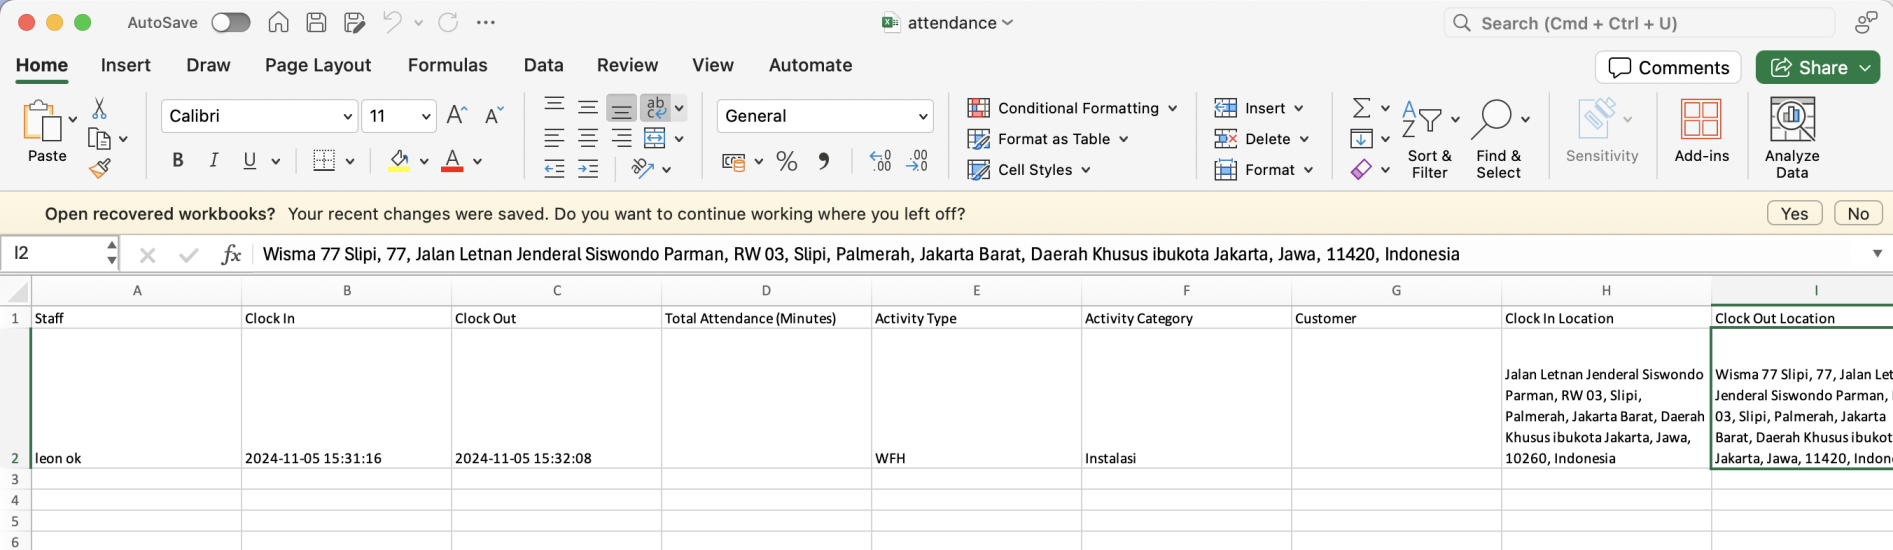
\includegraphics[width=8cm]{Gambar/bab3/user-manual/user-manual-file-excel-riwayat-presensi.png}
    	\caption{\textit{File Excel} Riwayat Presensi}
    	\label{fig:user-manual-file-excel-riwayat-presensi}
        \end{figure}
        \FloatBarrier
    \end{enumerate}

    \item Melihat Riwayat Lembur\label{item:melihat-riwayat-lembur}
    \begin{enumerate}
        \item Melakukan \textit{login} pada aplikasi presensi \textit{online} yang terdapat pada \textbf{Manual \ref{item:melakukan-login}}.
        \item Menekan tombol "\textit{History}" pada \textit{navigation bar} yang terletak di paling atas dan memilih tombol \textit{"Overtime History"}. \textbf{\ref{fig:user-manual-tombol-overtime-history-pada-navigation-bar}} menunjukkan tombol \textit{"Overtime History"} pada \textit{navigation bar}.
        \begin{figure}[!htbp]
    	\centering
    	
\includegraphics[width=8cm]{Gambar/bab3/user-manual/user-manual-navbar-overtime-history.png}
    	\caption{Tombol \textit{Overtime History} Pada \textit{Navigation Bar}}
    	\label{fig:user-manual-tombol-overtime-history-pada-navigation-bar}
        \end{figure}
        \FloatBarrier
        \item Seluruh daftar data riwayat lembur akan ditampilkan pada halaman \textit{overtime history}. \textbf{\ref{fig:user-manual-halaman-riwayat-lembur}} menunjukkan halaman \textit{overtime history}. 
        \begin{figure}[!htbp]
    	\centering
    	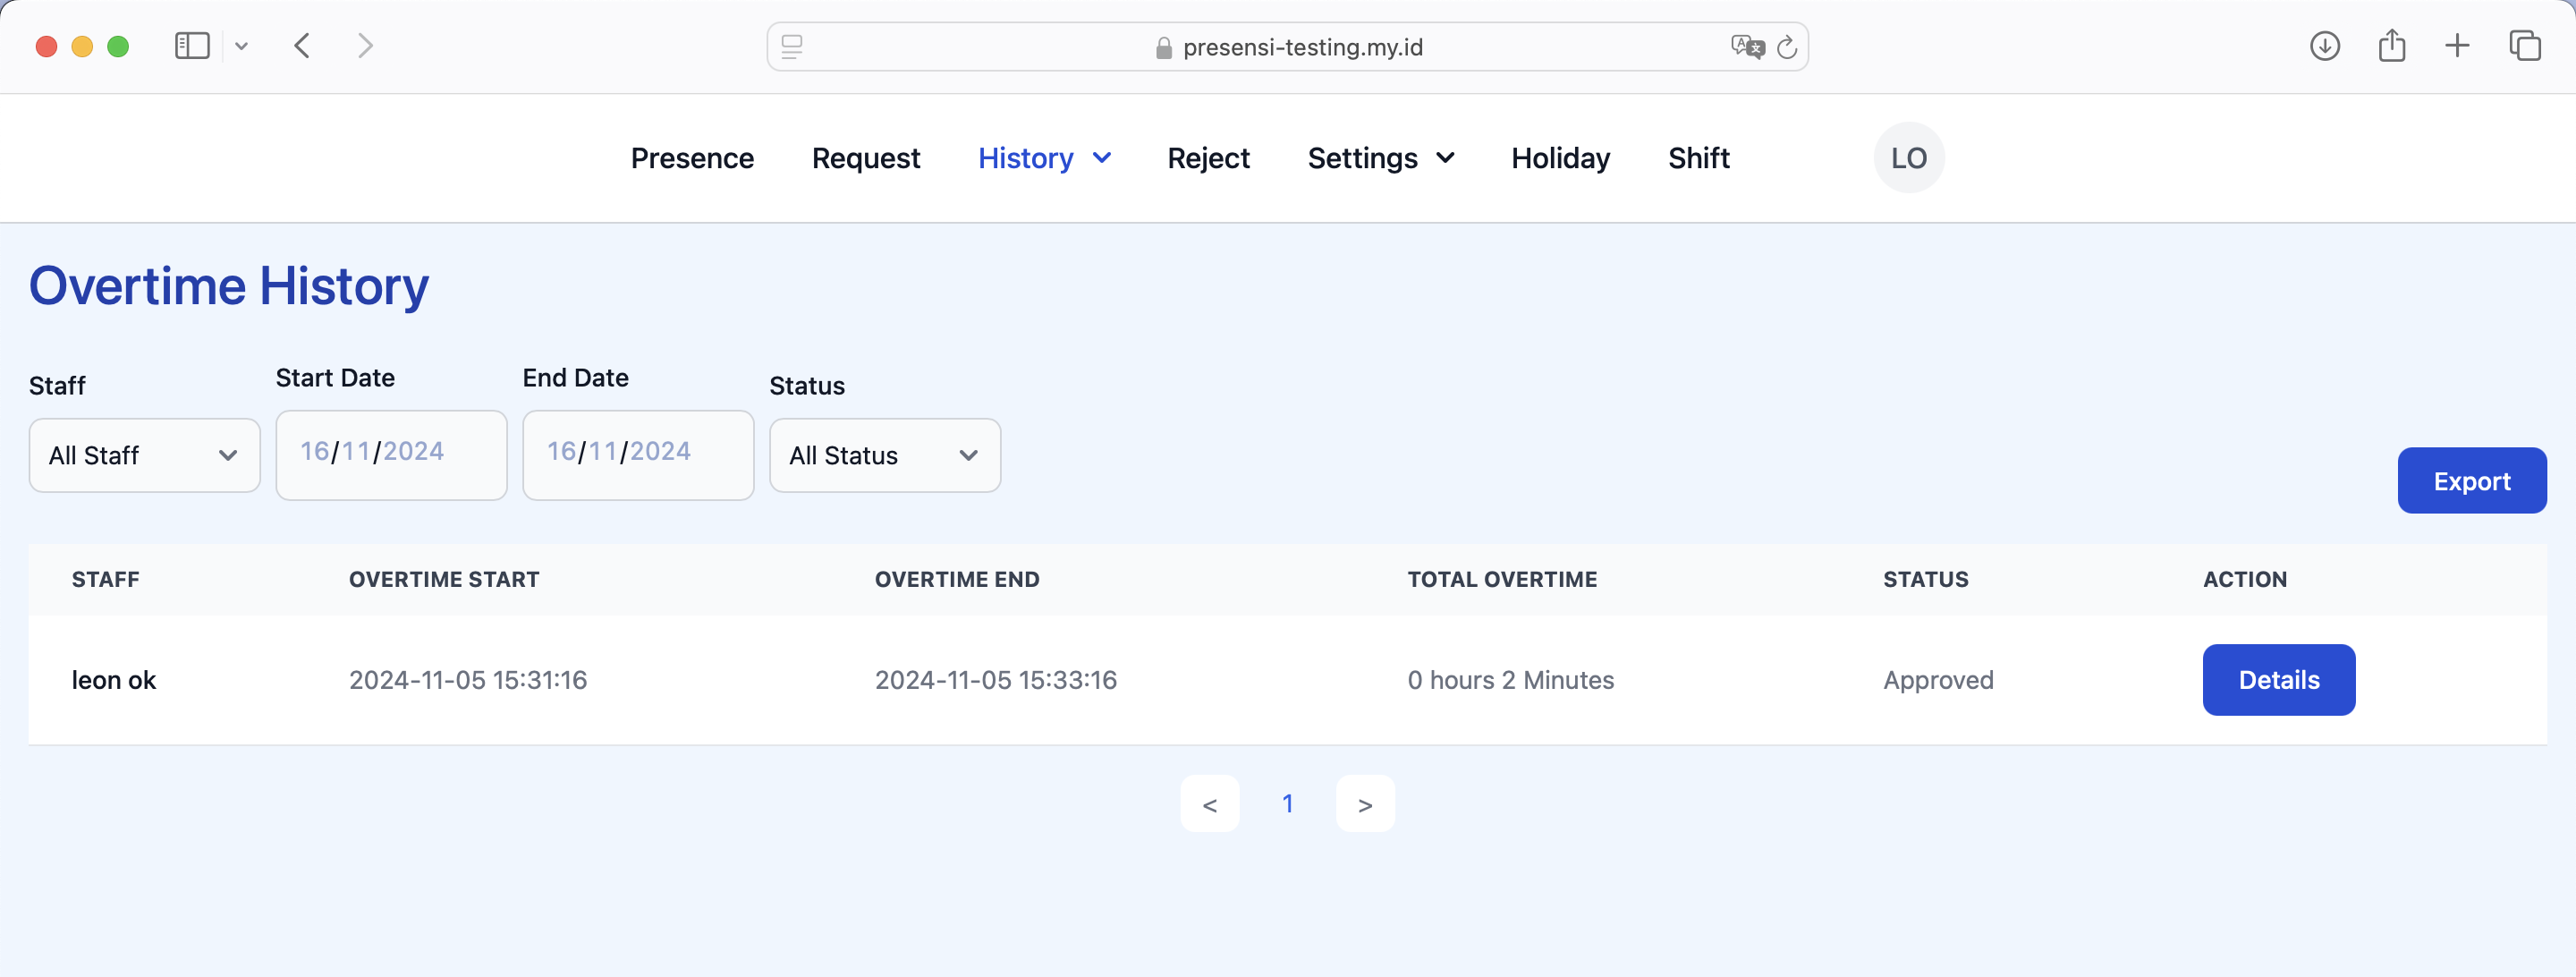
\includegraphics[width=8cm]{Gambar/bab3/user-manual/user-manual-halaman-riwayat-lembur.png}
    	\caption{Halaman \textit{Overtime History}}
    	\label{fig:user-manual-halaman-riwayat-lembur}
        \end{figure}
        \FloatBarrier
    \end{enumerate}

    \item Melihat Detail Riwayat Lembur
    \begin{enumerate}
        \item Membuka halaman riwayat lembur yang terdapat pada \textbf{Manual \ref{item:melihat-riwayat-lembur}}.
        \item Menekan tombol "\textit{Detail}" pada salah satu data lembur. Sistem akan menampilkan modal detail riwayat lembur beserta informasi lengkap riwayat lembur. \textbf{\ref{fig:user-manual-modal-overtime-history-details}} menunjukkan modal \textit{overtime history details}.
        \begin{figure}[!htbp]
    	\centering
    	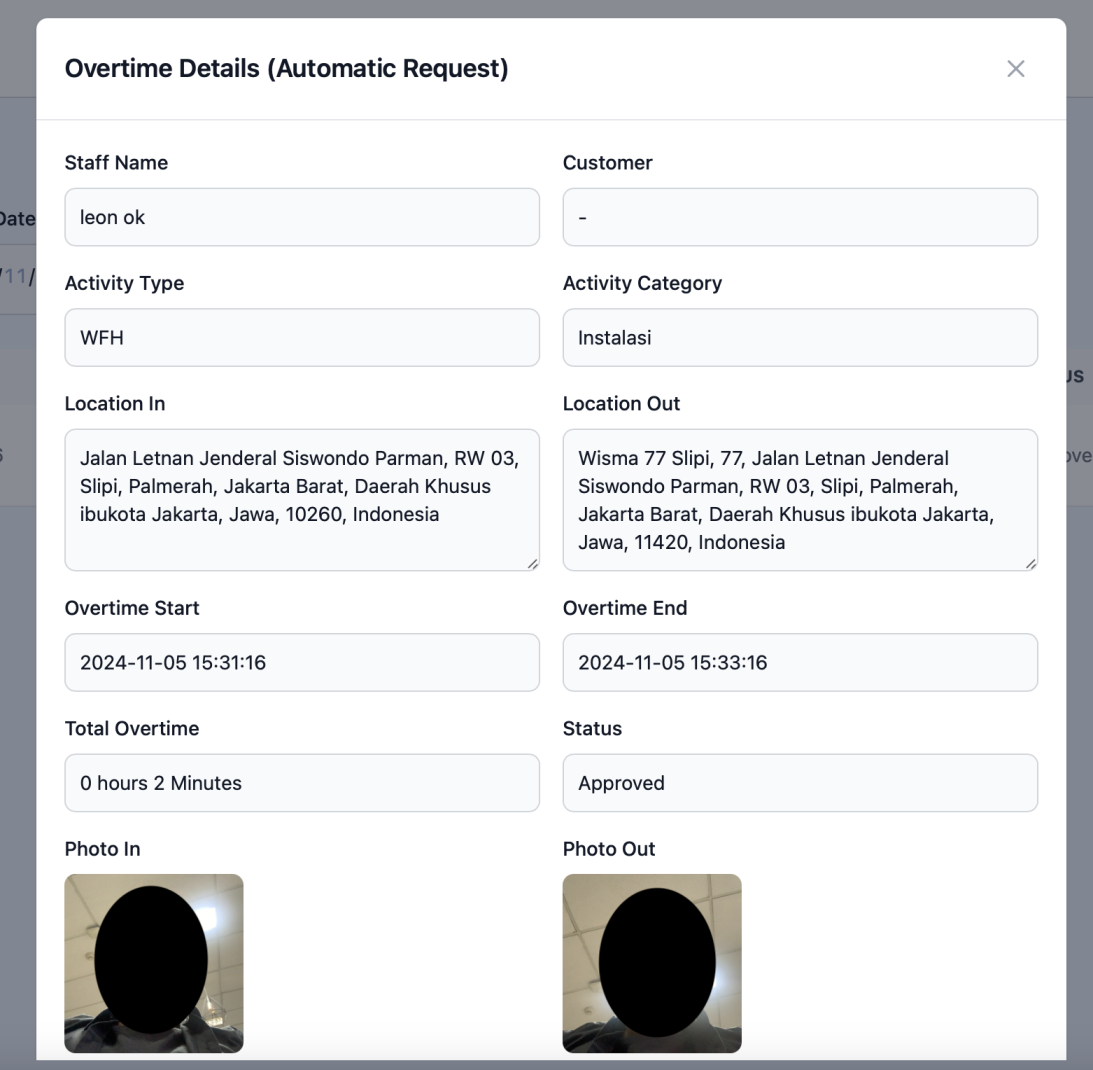
\includegraphics[width=8cm]{Gambar/bab3/user-manual/user-manual-detail-riwayat-lembur.png}
    	\caption{Modal \textit{Overtime History Details}}
    	\label{fig:user-manual-modal-overtime-history-details}
        \end{figure}
        \FloatBarrier
    \end{enumerate}

    \item Melakukan \textit{Export} Data Riwayat Lembur
    \begin{enumerate}
        \item Membuka halaman riwayat lembur yang terdapat pada \textbf{Manual \ref{item:melihat-riwayat-lembur}}.
        \item Menekan tombol \textit{"Export"} yang terdapat pada halaman riwayat lembur. \textbf{\ref{fig:user-manual-tombol-export-riwayat-lembur}} menunjukkan tombol untuk \textit{export} riwayat lembur menjadi format \textit{Excel}.
        \begin{figure}[!htbp]
    	\centering
    	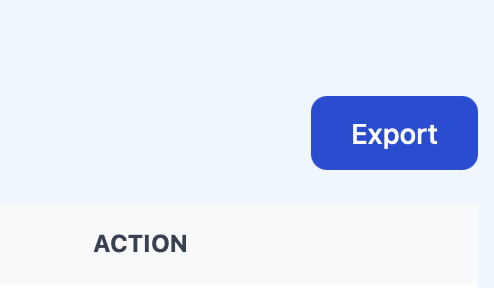
\includegraphics[width=8cm]{Gambar/bab3/user-manual/user-manual-tombol-export-riwayat-lembur.png}
    	\caption{Tombol \textit{Export} Riwayat Lembur}
    	\label{fig:user-manual-tombol-export-riwayat-lembur}
        \end{figure}
        \FloatBarrier
        \item Perangkat akan otomatis men-\textit{download file Excel} yang berisi data lembur. \textbf{\ref{fig:user-manual-file-excel-riwayat-lembur}} menunjukkan \textit{file Excel} riwayat lembur yang telah di-\textit{donwload}.
        \begin{figure}[!htbp]
    	\centering
    	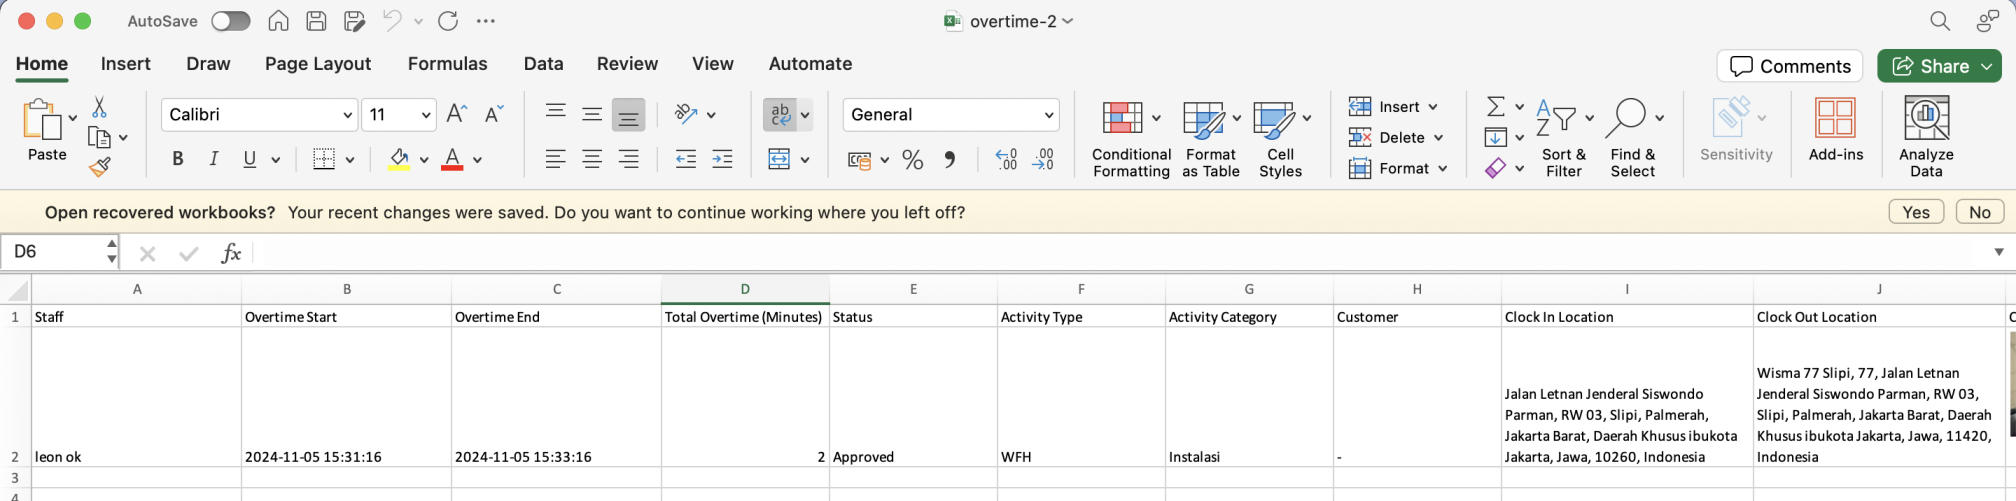
\includegraphics[width=8cm]{Gambar/bab3/user-manual/user-manual-file-excel-riwayat-lembur.png}
    	\caption{\textit{File Excel} Riwayat Lembur}
    	\label{fig:user-manual-file-excel-riwayat-lembur}
        \end{figure}
        \FloatBarrier
    \end{enumerate}
    

    \item Mengakses Halaman \textit{Reject} Lembur\label{item:mengakses-halaman-reject}
    \begin{enumerate}
        \item Melakukan \textit{login} pada aplikasi presensi \textit{online} yang terdapat pada \textbf{Manual \ref{item:melakukan-login}}.
        \item Menekan tombol "\textit{Reject}" pada \textit{navigation bar} yang terletak di paling atas. \textbf{\ref{fig:user-manual-tombol-reject-pada-navigation-bar}} menunjukkan tombol \textit{"Reject"} pada \textit{navigation bar}.
        \begin{figure}[!htbp]
    	\centering
    	
\includegraphics[width=8cm]{Gambar/bab3/user-manual/user-manual-navbar-reject.png}
    	\caption{Tombol \textit{Reject} Pada \textit{Navigation Bar}}
    	\label{fig:user-manual-tombol-reject-pada-navigation-bar}
        \end{figure}
        \FloatBarrier
        \item Sistem akan menampilkan halaman \textit{reject} lembur. \textbf{\ref{fig:user-manual-halaman-reject-lembur}} menunjukkan tampilan halaman \textit{reject lembur}.
        \begin{figure}[!htbp]
    	\centering
    	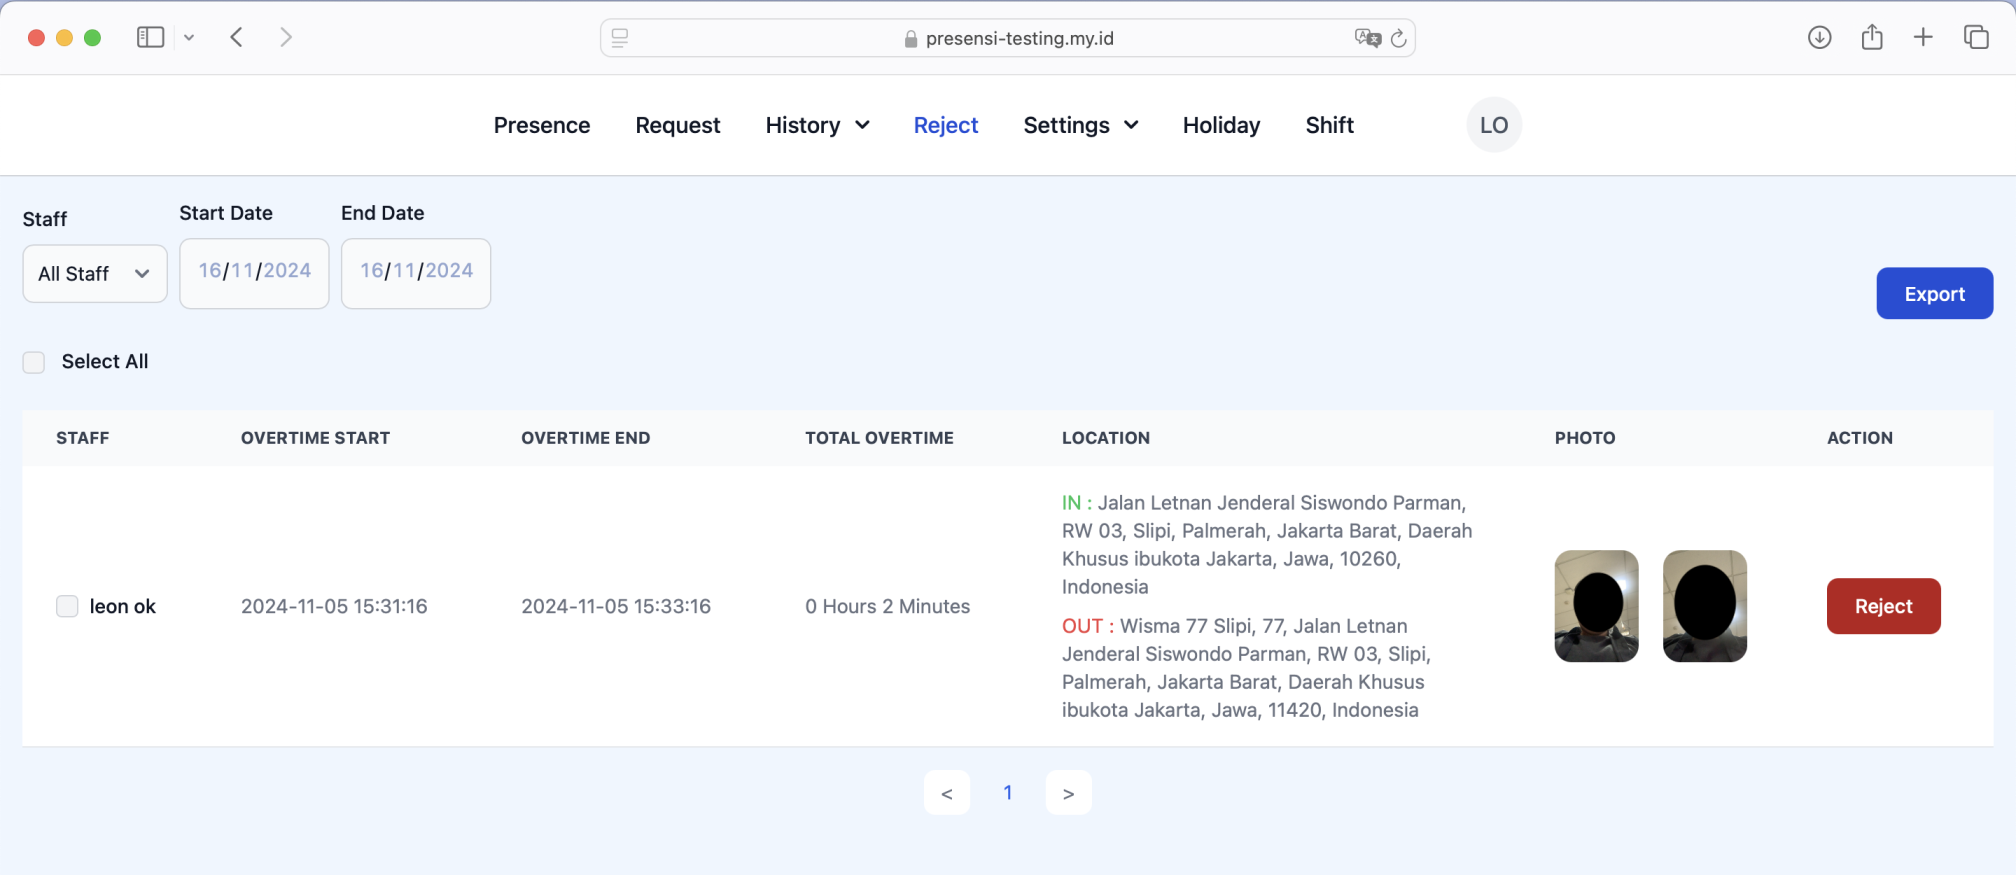
\includegraphics[width=8cm]{Gambar/bab3/user-manual/user-manual-halaman-reject-lembur.png}
    	\caption{Halaman \textit{Reject} Lembur}
    	\label{fig:user-manual-halaman-reject-lembur}
        \end{figure}
        \FloatBarrier
    \end{enumerate}

    \item Melakukan \textit{Reject} Satu Data Lembur
    \begin{enumerate}
        \item Membuka halaman \textit{reject} lembur yang terdapat pada \textbf{Manual \ref{item:mengakses-halaman-reject}}.
        \item Menekan tombol \textit{"Reject"} pada salah satu data lembur dan melakukan konfirmasi. \textbf{\ref{fig:user-manual-tombol-reject-data-lembur}} menunjukkan tombol \textit{"Reject"} pada salah satu data lembur.
        \begin{figure}[!htbp]
    	\centering
    	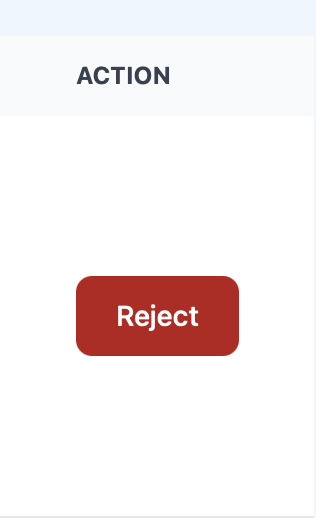
\includegraphics[width=5cm]{Gambar/bab3/user-manual/user-manual-tombol-reject-satu-data-lembur.png}
    	\caption{Tombol \textit{Reject} Pada Data Lembur}
    	\label{fig:user-manual-tombol-reject-data-lembur}
        \end{figure}
        \FloatBarrier
    \end{enumerate}

    \item Melakukan \textit{"Reject"} Lebih Dari Satu Data Lembur
    \begin{enumerate}
        \item Membuka halaman \textit{reject} lembur yang terdapat pada \textbf{Manual \ref{item:mengakses-halaman-reject}}.
        \item Melakukan centang pada \textit{checkbox} data lembur yang akan di-\textit{reject}. \textbf{\ref{fig:user-manual-checkbox-data-lembur}} menunjukkan \textit{checkbox} pada salah satu data lembur.
        \begin{figure}[!htbp]
    	\centering
    	
\includegraphics[width=8cm]{Gambar/bab3/user-manual/user-manual-checkbox-reject-data-lembur.png}
    	\caption{\textit{Checkbox} Data Lembur}
    	\label{fig:user-manual-checkbox-data-lembur}
        \end{figure}
        \FloatBarrier
        \item Setelah memilih \textit{checkbox}, maka akan muncul tombol "\textit{Reject Selected}" untuk me-\textit{reject} seluruh data lembur yang dipilih. \textbf{\ref{fig:user-manual-tombol-reject-selected}} menunjukkan tombol \textit{"Reject Selected"} pada halaman \textit{reject} lembur.
        \begin{figure}[!htbp]
    	\centering
    	
\includegraphics[width=8cm]{Gambar/bab3/user-manual/user-manual-tombol-reject-selected.png}
    	\caption{Tombol \textit{Reject Selected}}
    	\label{fig:user-manual-tombol-reject-selected}
        \end{figure}
        \FloatBarrier
    \end{enumerate}

    \item Melakukan \textit{Export} Data Lembur Pada Halaman \textit{Reject} Lembur
    \begin{enumerate}
        \item Membuka halaman \textit{reject} lembur yang terdapat pada \textbf{Manual \ref{item:mengakses-halaman-reject}}.
        \item Menekan tombol \textit{"Export"} yang terdapat pada halaman \textit{reject} lembur. \textbf{\ref{fig:user-manual-tombol-export-pada-reject-lembur}} menunjukkan tombol "\textit{Export}" pada halaman \textit{reject} lembur.
        \begin{figure}[!htbp]
    	\centering
    	
\includegraphics[width=8cm]{Gambar/bab3/user-manual/user-manual-tombol-export-reject-lembur.png}
    	\caption{Tombol \textit{Export} Pada \textit{Reject} Lembur}
    	\label{fig:user-manual-tombol-export-pada-reject-lembur}
        \end{figure}
        \FloatBarrier
        \item Sistem akan otomatis mengunduh \textit{file Excel} yang berisi data lembur dengan status tidak ter-\textit{reject}. \textbf{\ref{fig:user-manual-file-excel-reject-lembur}} menunjukkan \textit{file Excel} yang berisi data lembur yang tidak ter-\textit{reject}.
        \begin{figure}[!htbp]
    	\centering
    	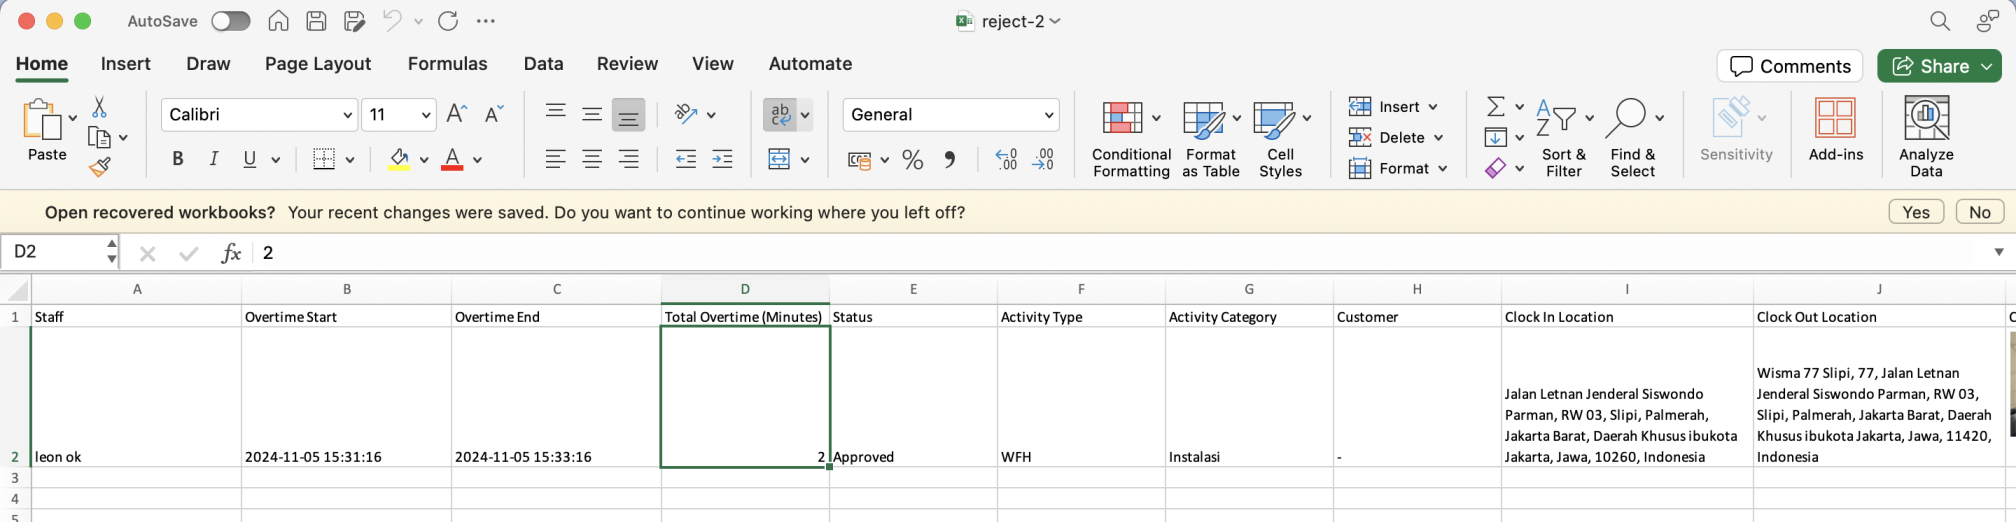
\includegraphics[width=8cm]{Gambar/bab3/user-manual/user-manual-file-excel-reject-lembur.png}
    	\caption{\textit{File Excel Reject} Lembur}
    	\label{fig:user-manual-file-excel-reject-lembur}
        \end{figure}
        \FloatBarrier
    \end{enumerate}

    \item Mengakses Halaman Pengaturan \textit{User}\label{item:mengakses-halaman-pengaturan-user}
    \begin{enumerate}
        \item Melakukan \textit{login} pada aplikasi presensi \textit{online} yang terdapat pada \textbf{Manual \ref{item:melakukan-login}}.
        \item Menekan tombol "\textit{Settings}" pada \textit{navigation bar} yang terletak di paling atas, kemudian tekan tombol "\textit{User}". \textbf{\ref{fig:user-manual-tombol-pengaturan-user-navigation-bar}} menunjukkan tombol \textit{"User"} pada \textit{navigation bar}.
        \begin{figure}[!htbp]
    	\centering
    	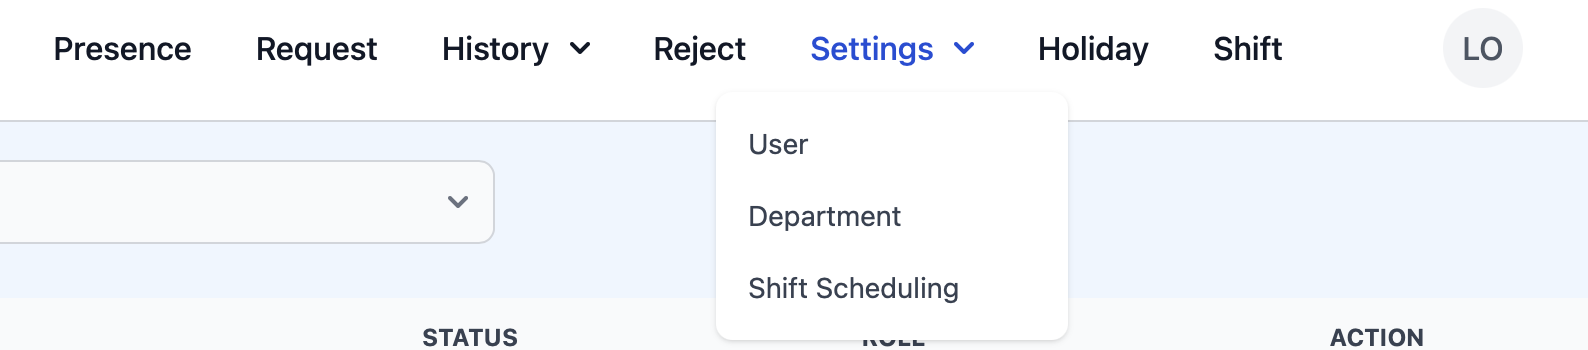
\includegraphics[width=8cm]{Gambar/bab3/user-manual/user-manual-navbar-user.png}
    	\caption{Tombol Pengaturan \textit{User} Pada \textit{Navigation Bar}}
    	\label{fig:user-manual-tombol-pengaturan-user-navigation-bar}
        \end{figure}
        \FloatBarrier
        \item Sistem akan menampilkan data \textit{user} pada halaman pengaturan \textit{user}. \textbf{\ref{fig:user-manual-halaman-pengaturan-user}} menunjukkan halaman pengaturan \textit{user}.
        \begin{figure}[!htbp]
    	\centering
    	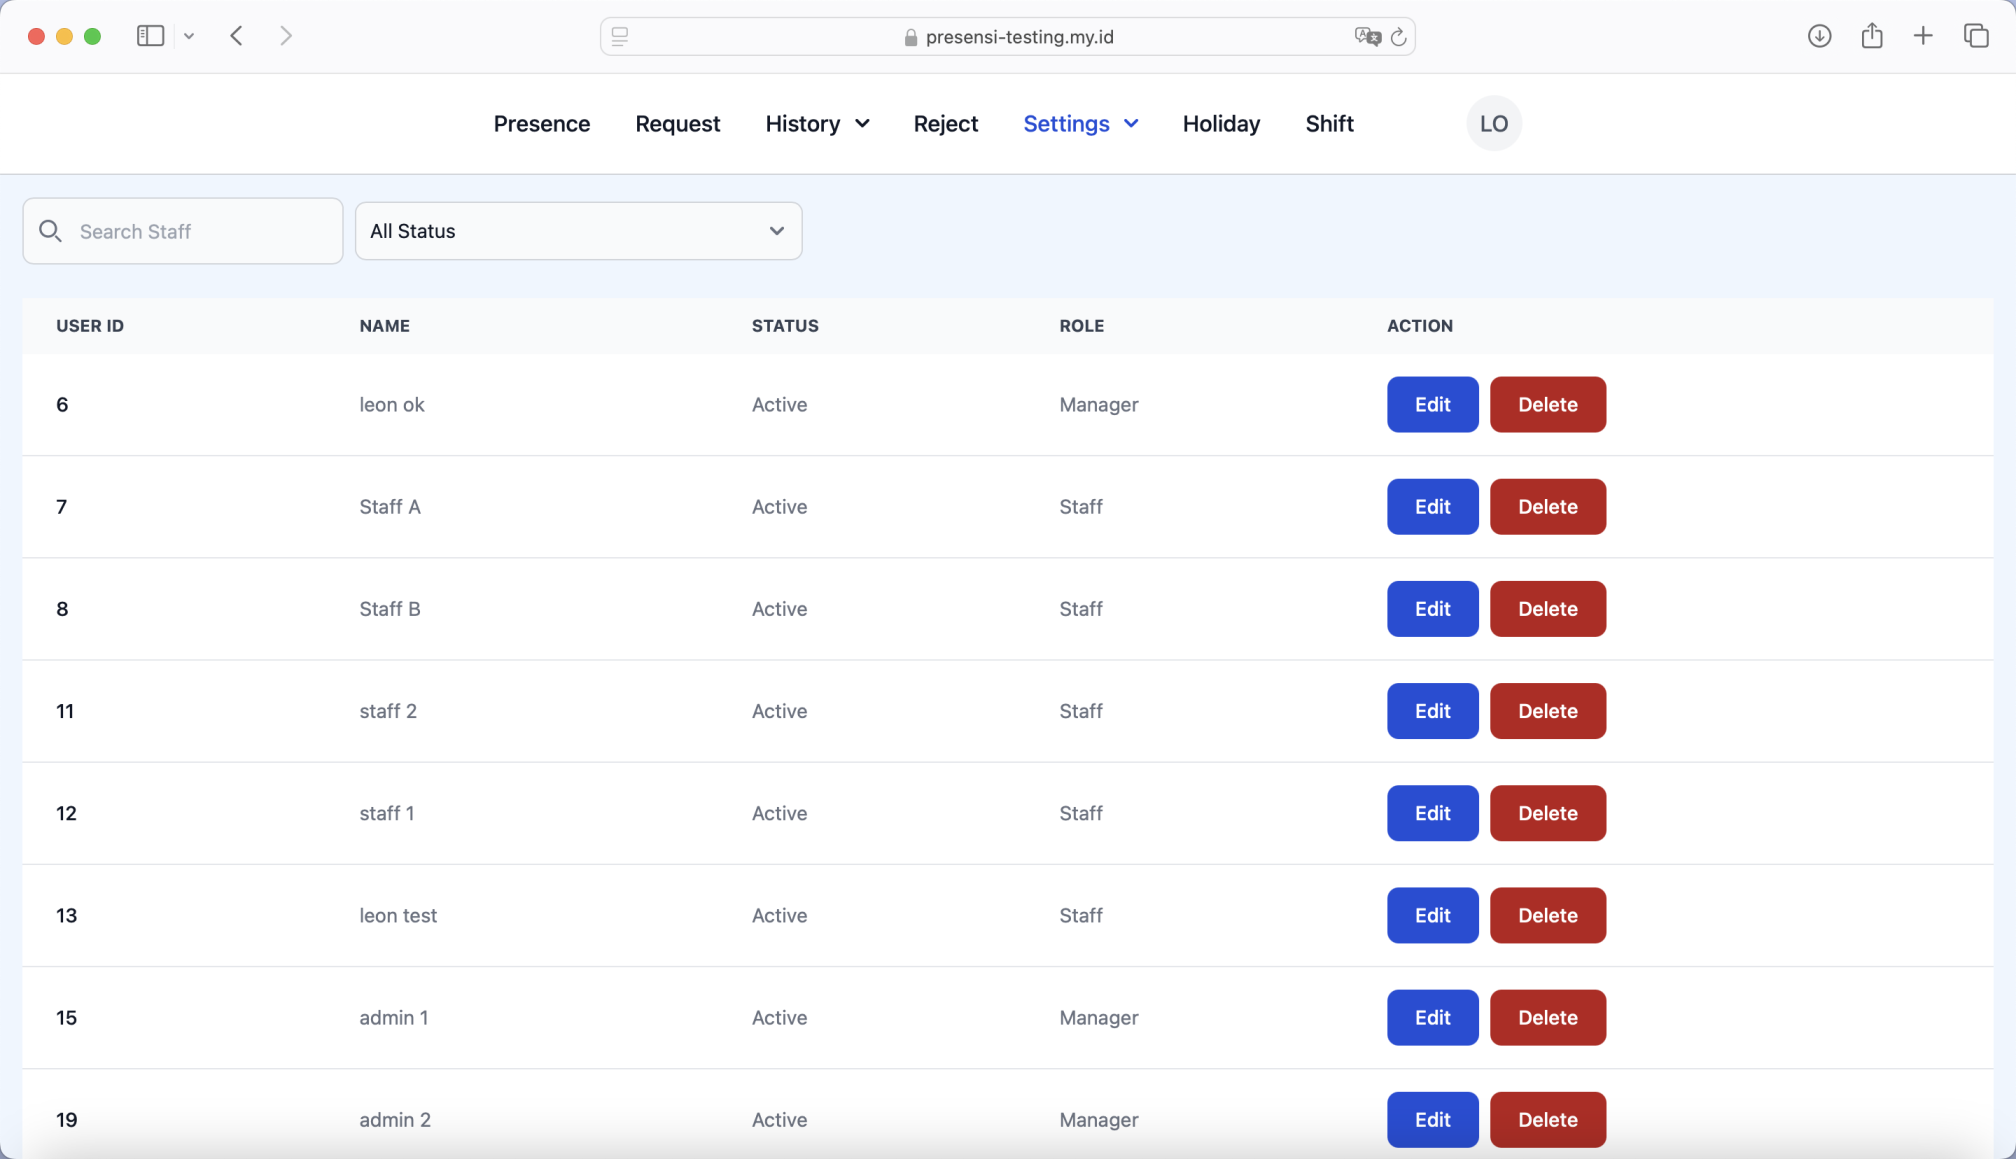
\includegraphics[width=8cm]{Gambar/bab3/user-manual/user-manual-halaman-user.png}
    	\caption{Halaman Pengaturan \textit{User}}
    	\label{fig:user-manual-halaman-pengaturan-user}
        \end{figure}
        \FloatBarrier
    \end{enumerate}

    \item Mengubah Data \textit{User}
    \begin{enumerate}
        \item Membuka halaman pengaturan \textit{user} yang terdapat pada \textbf{Manual \ref{item:mengakses-halaman-pengaturan-user}}. \textbf{\ref{fig:user-manual-tombol-edit-pada-data-user}} menunjukkan tombol "\textit{Edit}" pada data \textit{user}.
        \item Menekan tombol \textit{"Edit"} pada salah satu data \textit{user}.
        \begin{figure}[!htbp]
    	\centering
    	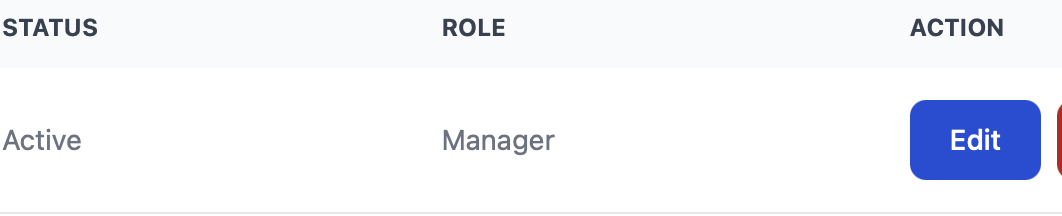
\includegraphics[width=8cm]{Gambar/bab3/user-manual/user-manual-tombol-edit-user.png}
    	\caption{Tombol \textit{Edit} Pada Data \textit{User}}
    	\label{fig:user-manual-tombol-edit-pada-data-user}
        \end{figure}
        \FloatBarrier
        \item Mengubah data \textit{user} melalui \textit{input form} pada modal \textit{edit user}, kemudian tekan tombol "\textit{Save Changes}" untuk menyimpan perubahan data. \textbf{\ref{fig:user-manual-modal-edit-user}} menunjukkan modal \textit{edit user}.
        \begin{figure}[!htbp]
    	\centering
    	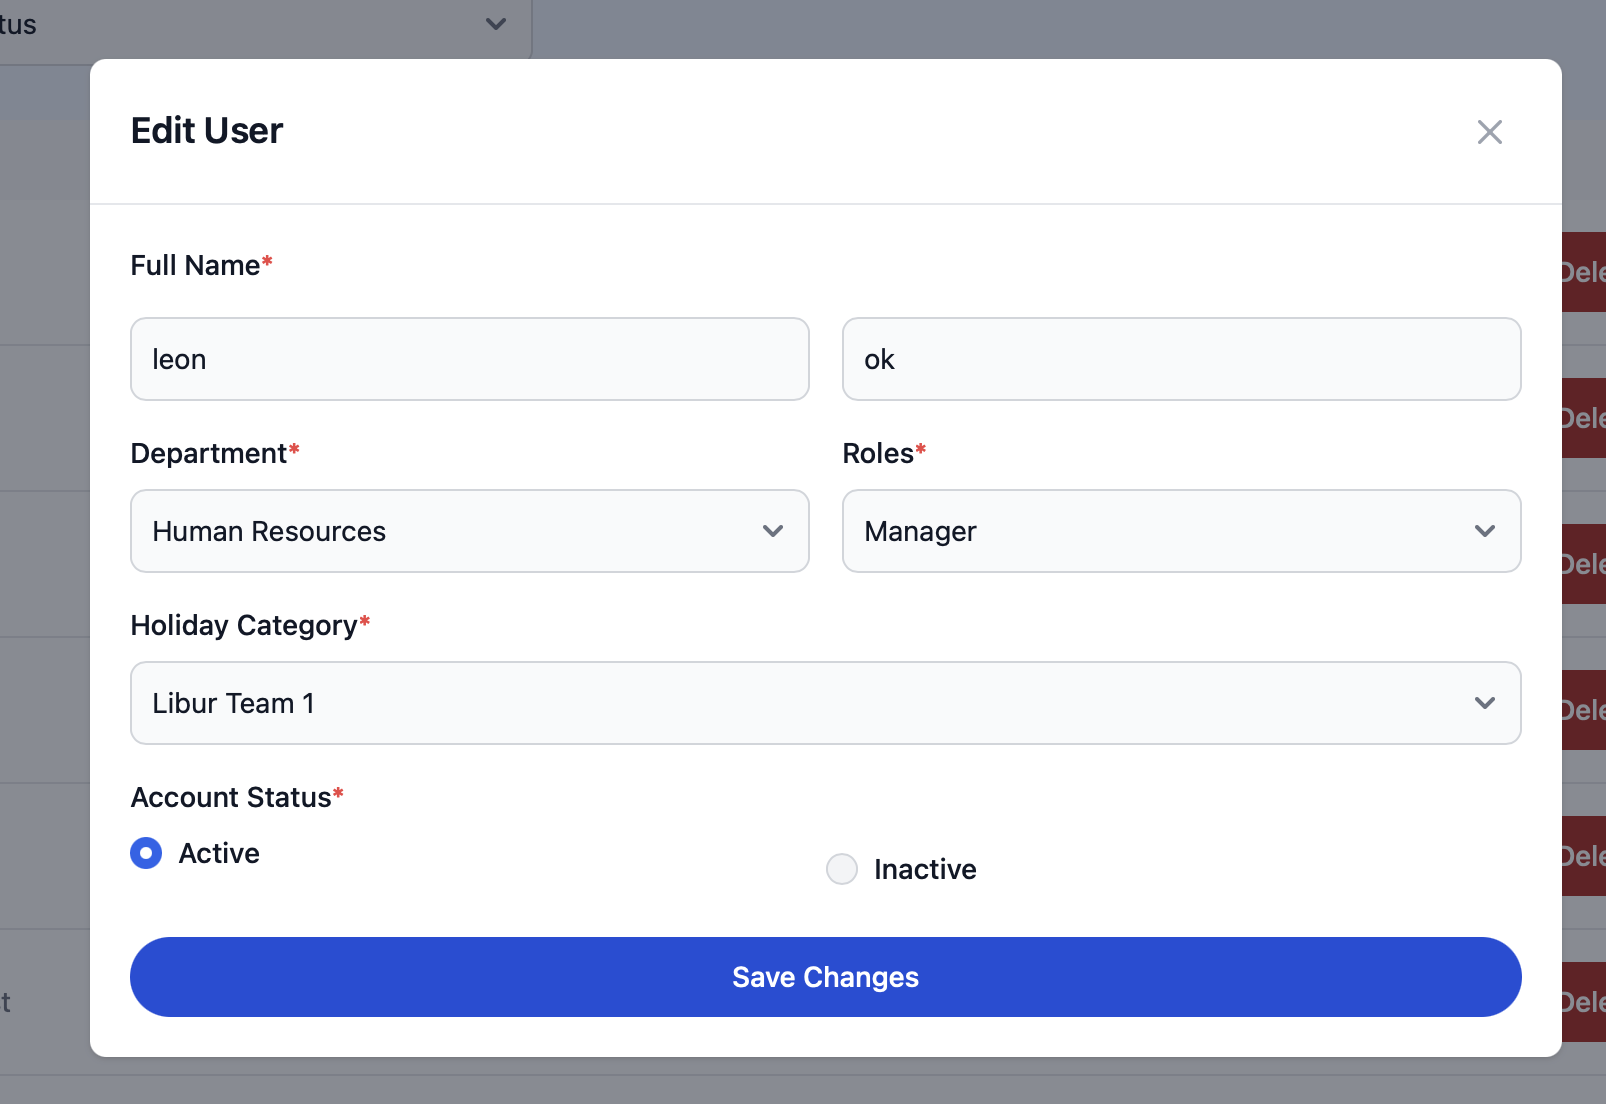
\includegraphics[width=8cm]{Gambar/bab3/user-manual/user-manual-modal-edit-user.png}
    	\caption{Modal \textit{Edit} \textit{User}}
    	\label{fig:user-manual-modal-edit-user}
        \end{figure}
        \FloatBarrier
    \end{enumerate}

    \item Menghapus Data \textit{User}
    \begin{enumerate}
        \item Membuka halaman pengaturan \textit{user} yang terdapat pada \textbf{Manual \ref{item:mengakses-halaman-pengaturan-user}}.
        \item Menekan tombol "\textit{Delete}" pada salah satu data \textit{user} dan lakukan konfirmasi penghapusan. \textbf{\ref{fig:user-manual-tombol-delete-user}} menunjukkan tombol "\textit{Delete}" untuk menghapus data \textit{user}.
        \begin{figure}[!htbp]
    	\centering
    	
\includegraphics[width=8cm]{Gambar/bab3/user-manual/user-manual-tombol-delete-user.png}
    	\caption{Tombol \textit{Delete User}}
    	\label{fig:user-manual-tombol-delete-user}
        \end{figure}
        \FloatBarrier
    \end{enumerate}

    \item Mengakses Halaman \textit{Department}\label{item:mengakses-department}
    \begin{enumerate}
        \item Melakukan \textit{login} pada aplikasi presensi \textit{online} yang terdapat pada \textbf{Manual \ref{item:melakukan-login}}.
        \item Menekan tombol "\textit{Settings}" pada \textit{navigation bar} yang terletak di paling atas, kemudian tekan tombol "\textit{Department}". \textbf{\ref{fig:user-manual-tombol-pengaturan-department-navigation-bar}} menunjukkan tombol \textit{"Department"} pada \textit{navigation bar}.
        \begin{figure}[!htbp]
    	\centering
    	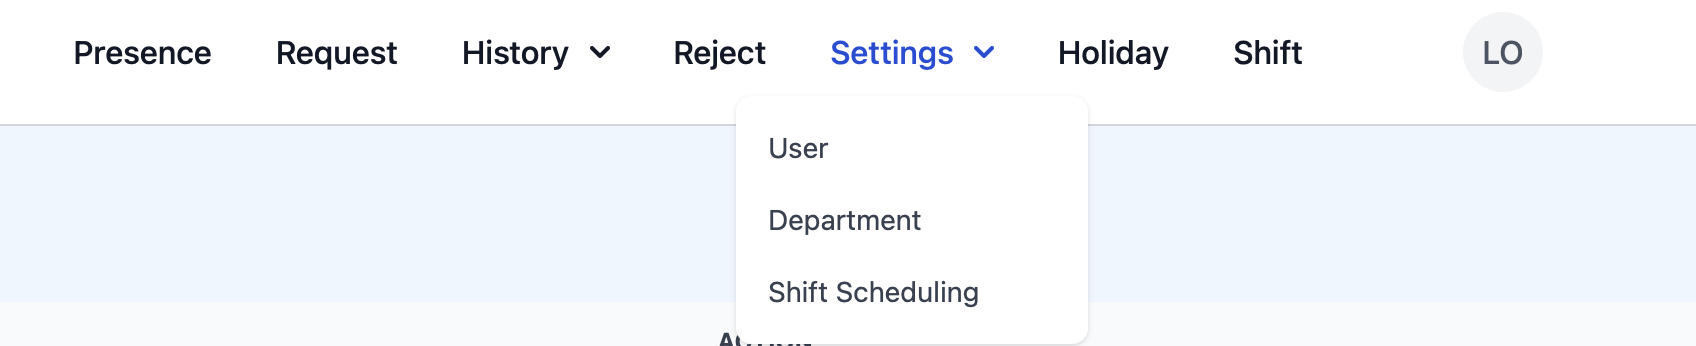
\includegraphics[width=8cm]{Gambar/bab3/user-manual/user-manual-navbar-department.png}
    	\caption{Tombol Pengaturan \textit{Department} Pada \textit{Navigation Bar}}
    	\label{fig:user-manual-tombol-pengaturan-department-navigation-bar}
        \end{figure}
        \FloatBarrier
        \item Sistem akan menampilkan data \textit{department} pada halaman pengaturan \textit{department}. \textbf{\ref{fig:user-manual-halaman-pengaturan-department}} menunjukkan halaman pengaturan \textit{department}.
        \begin{figure}[!htbp]
    	\centering
    	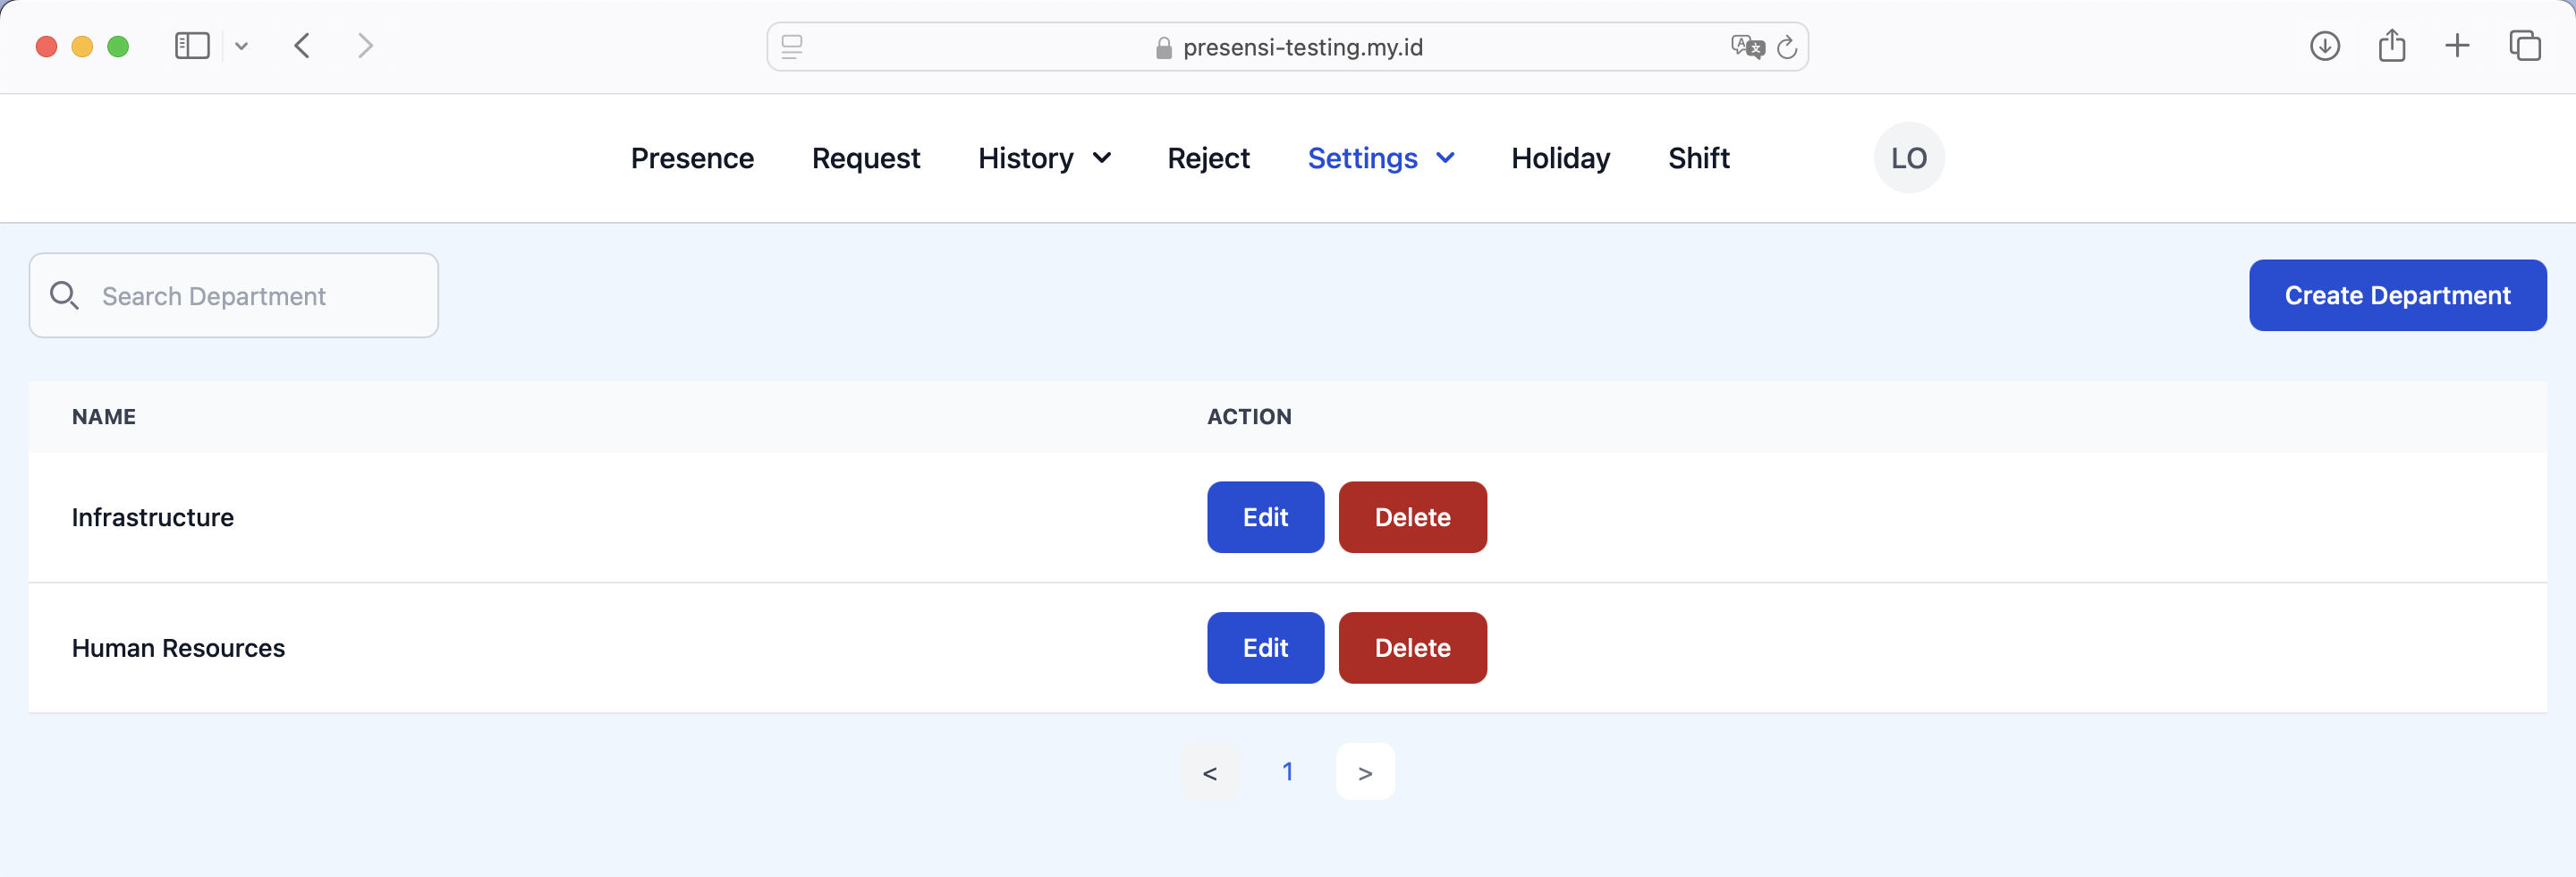
\includegraphics[width=8cm]{Gambar/bab3/user-manual/user-manual-halaman-department.png}
    	\caption{Halaman Pengaturan \textit{Department}}
    	\label{fig:user-manual-halaman-pengaturan-department}
        \end{figure}
        \FloatBarrier
    \end{enumerate}

    \item Menambah \textit{Department}
    \begin{enumerate}
        \item Membuka halaman pengaturan \textit{department} yang terdapat pada \textbf{Manual \ref{item:mengakses-department}}.
        \item Menekan tombol "\textit{Create Department}" pada halaman pengaturan \textit{department}. \textbf{\ref{fig:user-manual-tombol-create-new-department}} menunjukkan tombol "\textit{Create Department}" pada halaman pengaturan \textit{department}.
        \begin{figure}[!htbp]
    	\centering
    	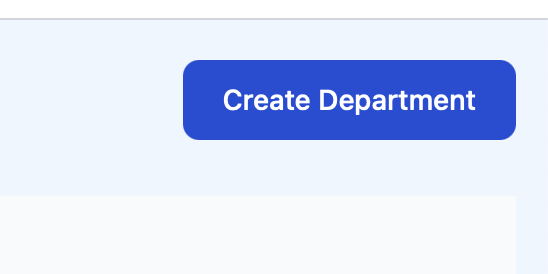
\includegraphics[width=8cm]{Gambar/bab3/user-manual/user-manual-tombol-create-new-department.png}
    	\caption{Tombol \textit{Create Department}}
    	\label{fig:user-manual-tombol-create-new-department}
        \end{figure}
        \FloatBarrier

        \item Mengisi seluruh \textit{input form} pada modal \textit{create new department}, kemudian tekan tombol "\textit{Create New Department}" untuk menyimpan data \textit{department} baru. \textbf{\ref{fig:user-manual-modal-create-new-department}} menunjukkan modal \textit{create new department}.
        \begin{figure}[!htbp]
    	\centering
    	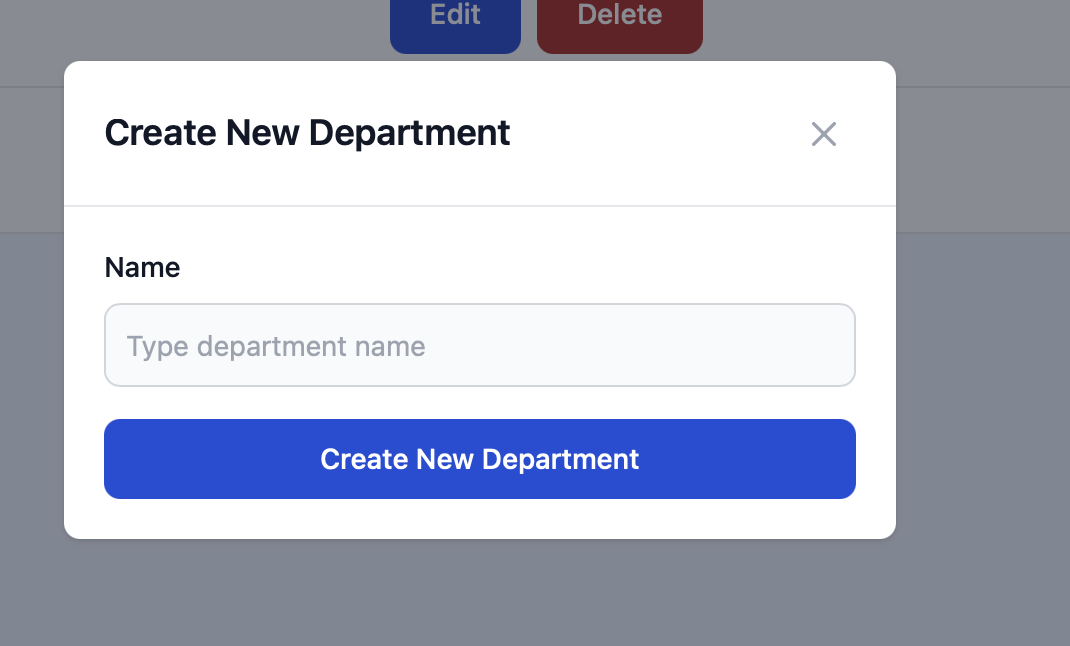
\includegraphics[width=8cm]{Gambar/bab3/user-manual/user-manual-modal-create-new-department.png}
    	\caption{Modal \textit{Create New Department}}
    	\label{fig:user-manual-modal-create-new-department}
        \end{figure}
        \FloatBarrier
    \end{enumerate}

    \item Mengubah \textit{Department}
    \begin{enumerate}
        \item Membuka halaman pengaturan \textit{department} yang terdapat pada \textbf{Manual \ref{item:mengakses-department}}.
        \item Menekan tombol "\textit{Edit}" salah satu data \textit{department} pada halaman pengaturan \textit{department}. \textbf{\ref{fig:user-manual-tombol-edit-department}} menunjukkan tombol "\textit{Edit}" pada halaman pengaturan \textit{department}.
        \begin{figure}[!htbp]
    	\centering
    	
\includegraphics[width=8cm]{Gambar/bab3/user-manual/user-manual-tombol-edit-department.png}
    	\caption{Tombol \textit{Edit} Department}
    	\label{fig:user-manual-tombol-edit-department}
        \end{figure}
        \FloatBarrier

        \item Mengubah seluruh \textit{input form} pada modal \textit{edit department}, kemudian tekan tombol "\textit{Save Changes}" untuk menyimpan data \textit{department}. \textbf{\ref{fig:user-manual-modal-edit-department}} menunjukkan modal \textit{edit department}.
        \begin{figure}[!htbp]
    	\centering
    	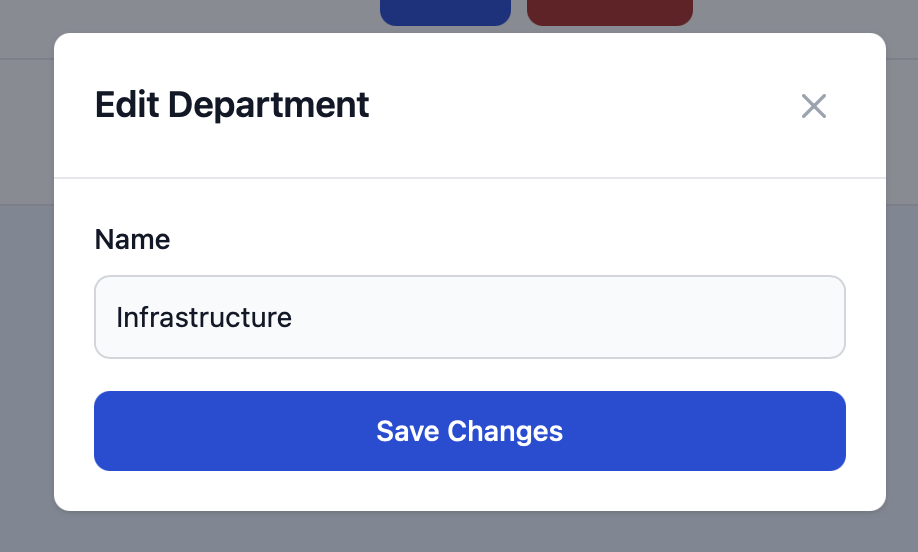
\includegraphics[width=8cm]{Gambar/bab3/user-manual/user-manual-modal-edit-department.png}
    	\caption{Modal \textit{Edit Department}}
    	\label{fig:user-manual-modal-edit-department}
        \end{figure}
        \FloatBarrier
    \end{enumerate}

    \item Menghapus Data \textit{Department}
    \begin{enumerate}
        \item Membuka halaman pengaturan \textit{department} yang terdapat pada \textbf{Manual \ref{item:mengakses-department}}.
        \item Menekan tombol "\textit{Delete}" pada salah satu data \textit{department} dan lakukan konfirmasi penghapusan. \textbf{\ref{fig:user-manual-tombol-delete-department}} menunjukkan tombol "\textit{Delete}" untuk menghapus data \textit{department}.
        \begin{figure}[!htbp]
    	\centering
    	
\includegraphics[width=8cm]{Gambar/bab3/user-manual/user-manual-tombol-delete-department.png}
    	\caption{Tombol \textit{Delete Department}}
    	\label{fig:user-manual-tombol-delete-department}
        \end{figure}
        \FloatBarrier
    \end{enumerate}

    \item Mengakses Halaman Penjadwalan \textit{Shift}\label{item:mengakses-shift-scheduling}
    \begin{enumerate}
        \item Melakukan \textit{login} pada aplikasi presensi \textit{online} yang terdapat pada \textbf{Manual \ref{item:melakukan-login}}.
        \item Menekan tombol "\textit{Settings}" pada \textit{navigation bar} yang terletak di paling atas, kemudian tekan tombol "\textit{Shift Scheduling}". \textbf{\ref{fig:user-manual-tombol-pengaturan-shift-scheduling-navigation-bar}} menunjukkan tombol \textit{"Shift Scheduling"} pada \textit{navigation bar}.
        \begin{figure}[!htbp]
    	\centering
    	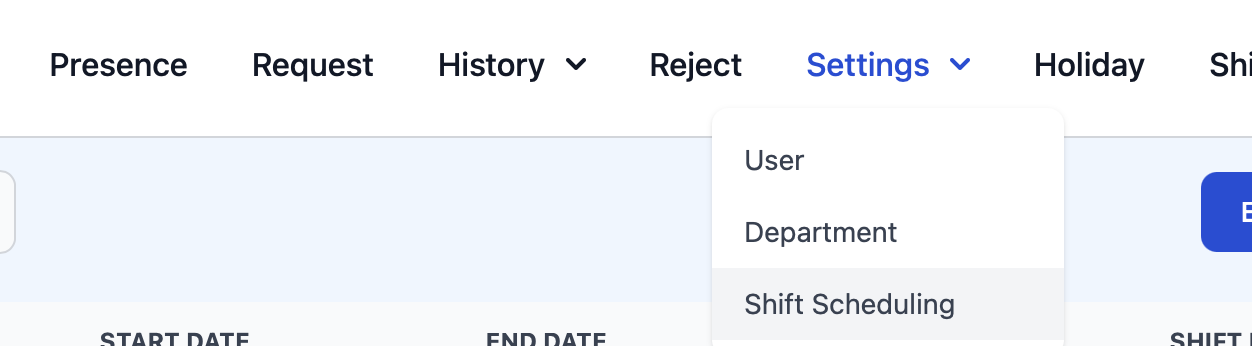
\includegraphics[width=8cm]{Gambar/bab3/user-manual/user-manual-navbar-shift-scheduling.png}
    	\caption{Tombol Pengaturan \textit{Shift Scheduling} Pada \textit{Navigation Bar}}
    	\label{fig:user-manual-tombol-pengaturan-shift-scheduling-navigation-bar}
        \end{figure}
        \FloatBarrier
        \item Sistem akan menampilkan data penjadwalan \textit{shift} pada halaman pengaturan \textit{shift scheduling}. \textbf{\ref{fig:user-manual-halaman-pengaturan-shift-scheduling}} menunjukkan halaman pengaturan \textit{shift scheduling}.
        \begin{figure}[!htbp]
    	\centering
    	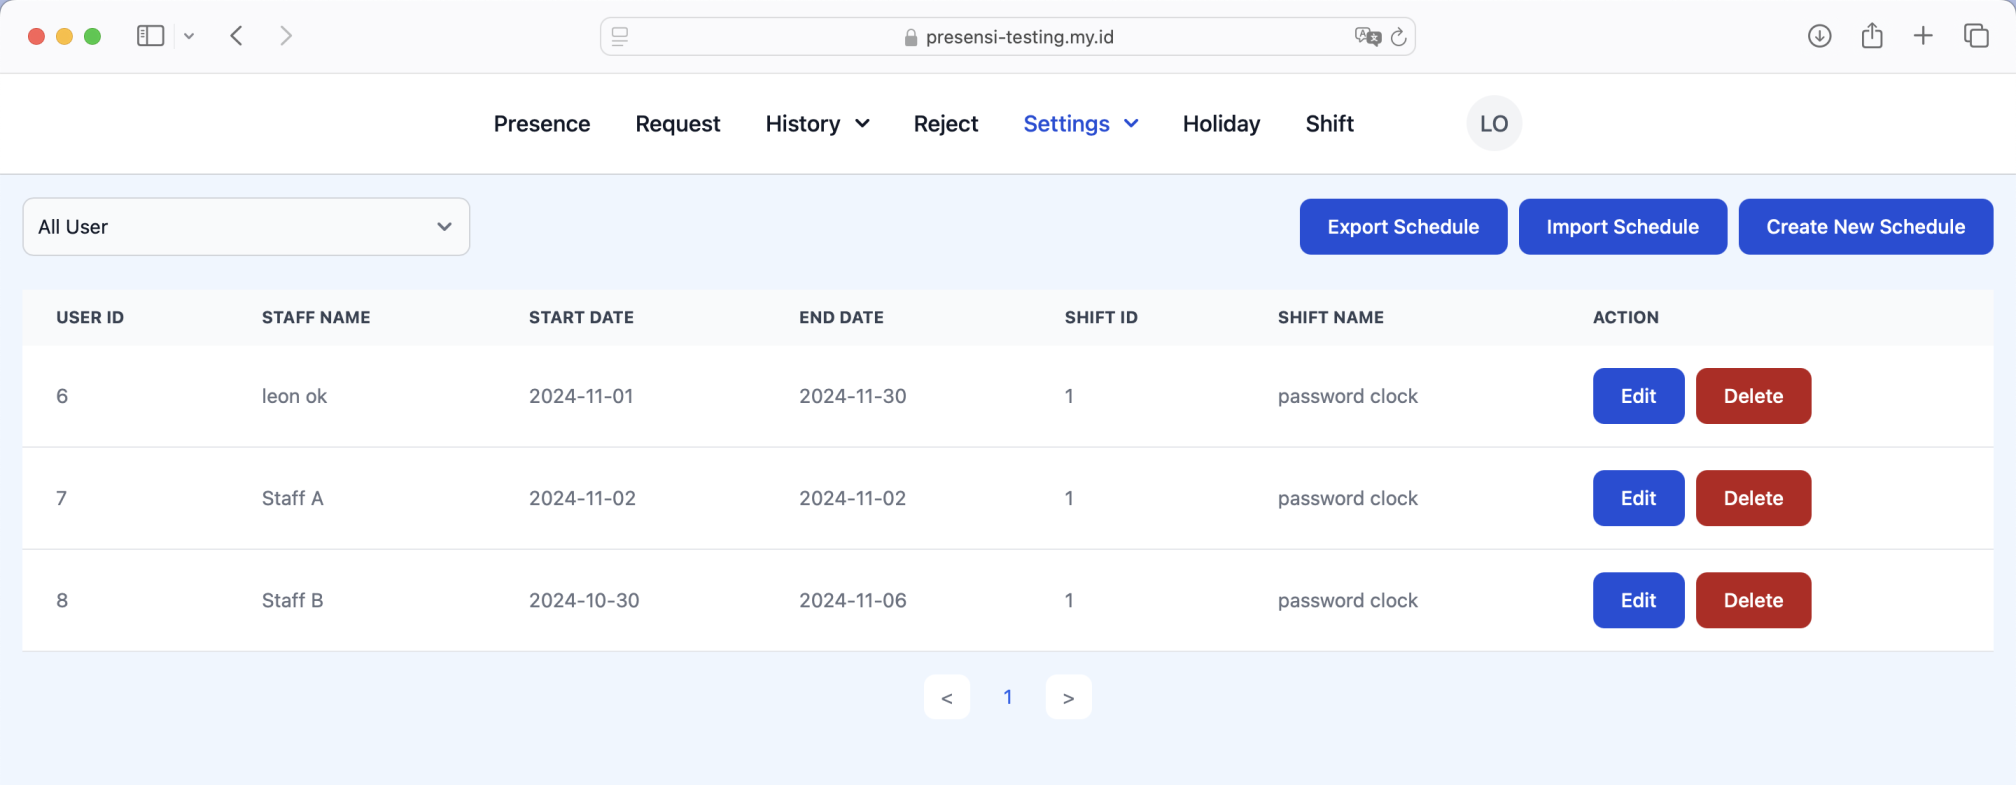
\includegraphics[width=8cm]{Gambar/bab3/user-manual/user-manual-halaman-shift-scheduling.png}
    	\caption{Halaman Pengaturan \textit{Shift Scheduling}}
    	\label{fig:user-manual-halaman-pengaturan-shift-scheduling}
        \end{figure}
        \FloatBarrier
    \end{enumerate}

    \item Menambah Data Penjadwalan \textit{Shift}
    \begin{enumerate}
        \item Membuka halaman \textit{shift scheduling} yang terdapat pada \textbf{Manual \ref{item:mengakses-shift-scheduling}}.
        \item Menekan tombol "\textit{Create New Schedule}" pada halaman pengaturan \textit{shift scheduling}. \textbf{\ref{fig:user-manual-tombol-create-new-schedule}} menunjukkan tombol "\textit{Create New Schedule}" pada halaman pengaturan \textit{shift scheduling}.
        \begin{figure}[!htbp]
    	\centering
    	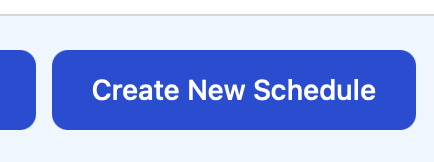
\includegraphics[width=8cm]{Gambar/bab3/user-manual/user-manual-tombol-create-new-schedule.png}
    	\caption{Tombol \textit{Create New Schedule}}
    	\label{fig:user-manual-tombol-create-new-schedule}
        \end{figure}
        \FloatBarrier

        \item Mengisi seluruh \textit{input form} pada modal \textit{create new schedule}, kemudian tekan tombol "\textit{Create New Schedule}" untuk menyimpan data penjadwalan \textit{shift} baru. \textbf{\ref{fig:user-manual-modal-create-new-schedule}} menunjukkan modal \textit{create new schedule}.
        \begin{figure}[!htbp]
    	\centering
    	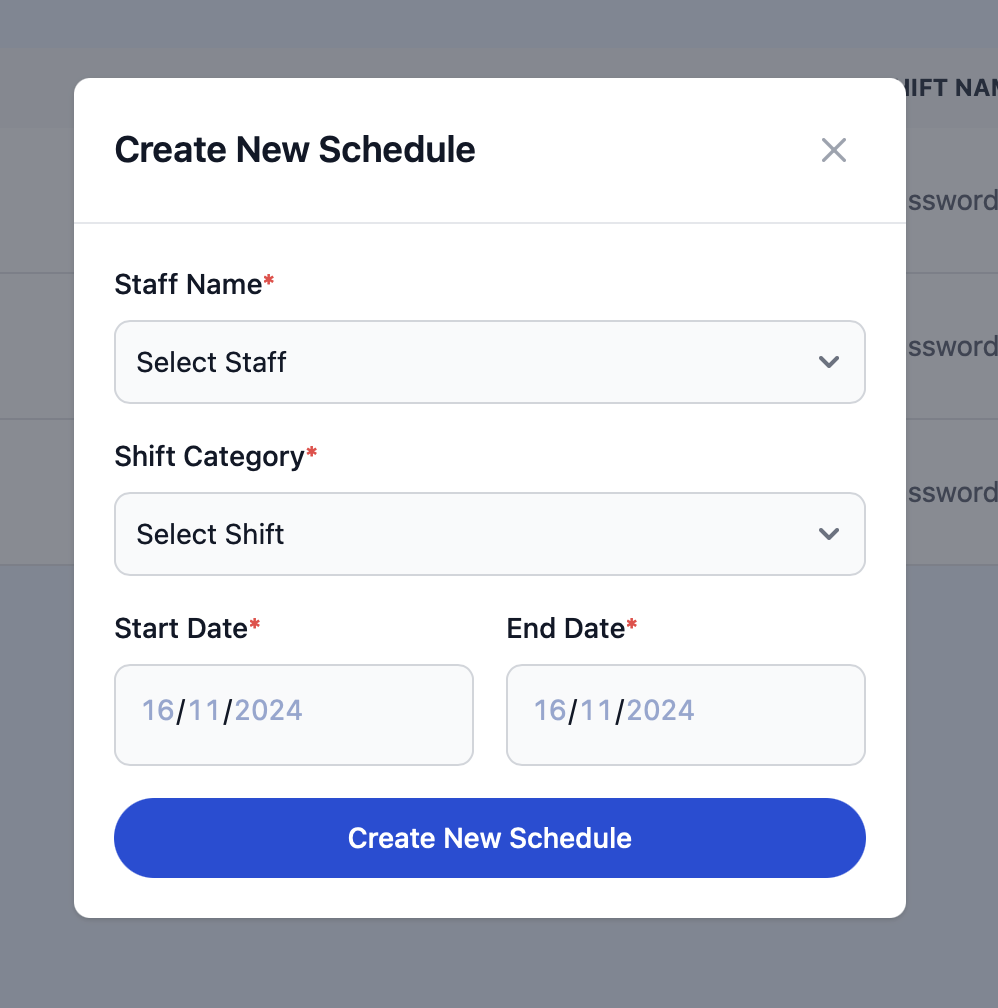
\includegraphics[width=8cm]{Gambar/bab3/user-manual/user-manual-modal-create-new-schedule.png}
    	\caption{Modal \textit{Create New Schedule}}
    	\label{fig:user-manual-modal-create-new-schedule}
        \end{figure}
        \FloatBarrier
    \end{enumerate}

    \item Mengubah Data Penjadwalan \textit{Shift}
    \begin{enumerate}
        \item Membuka halaman \textit{shift scheduling} yang terdapat pada \textbf{Manual \ref{item:mengakses-shift-scheduling}}.
        \item Menekan tombol "\textit{Edit}" salah satu data \textit{shift scheduling} pada halaman pengaturan \textit{shift scheduling}. \textbf{\ref{fig:user-manual-tombol-edit-schedule}} menunjukkan tombol "\textit{Edit}" pada halaman pengaturan \textit{shift scheduling}.
        \begin{figure}[!htbp]
    	\centering
    	
\includegraphics[width=8cm]{Gambar/bab3/user-manual/user-manual-tombol-edit-schedule.png}
    	\caption{Tombol \textit{Edit Schedule}}
    	\label{fig:user-manual-tombol-edit-schedule}
        \end{figure}
        \FloatBarrier

        \item Mengubah seluruh \textit{input form} pada modal \textit{edit schedule}, kemudian tekan tombol "\textit{Edit Schedule}" untuk menyimpan data \textit{shift scheduling}. \textbf{\ref{fig:user-manual-modal-edit-schedule}} menunjukkan modal \textit{edit schedule}.
        \begin{figure}[!htbp]
    	\centering
    	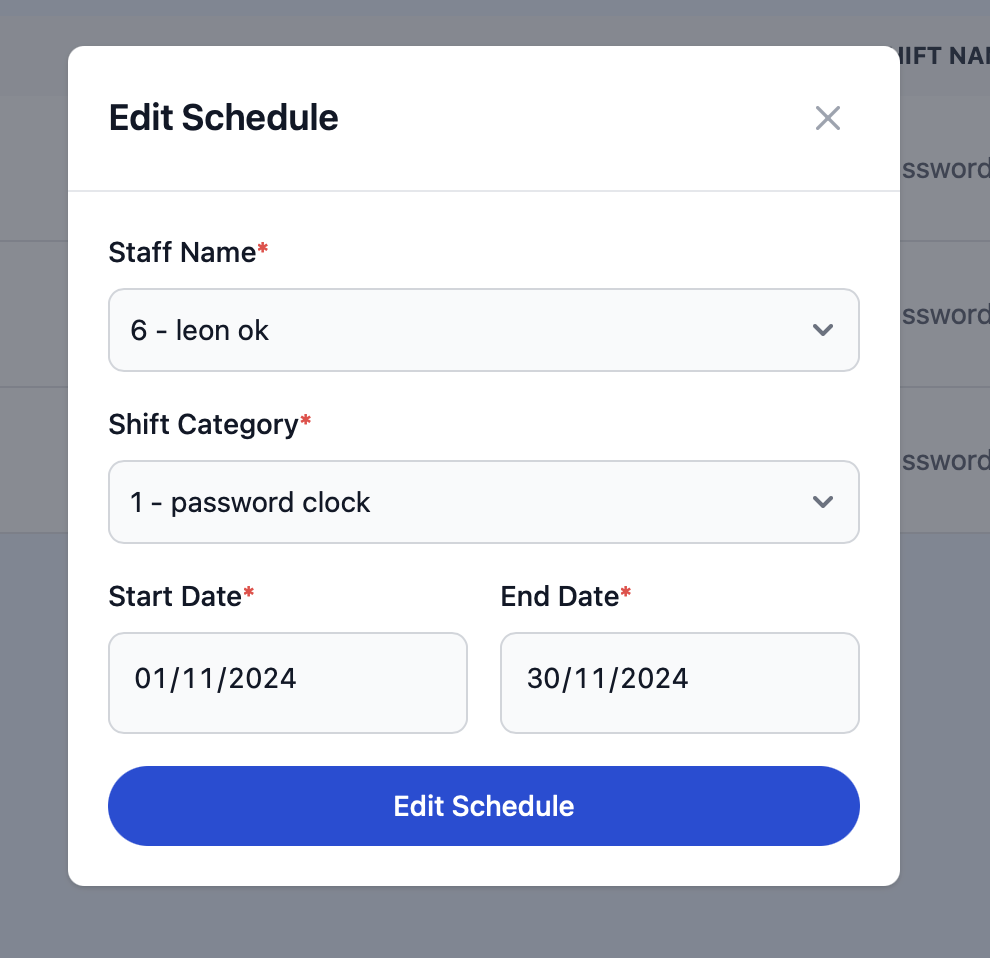
\includegraphics[width=8cm]{Gambar/bab3/user-manual/user-manual-modal-edit-schedule.png}
    	\caption{Modal \textit{Edit Schedule}}
    	\label{fig:user-manual-modal-edit-schedule}
        \end{figure}
        \FloatBarrier
    \end{enumerate}

    \item Menghapus Data Penjadwalan \textit{Shift}
    \begin{enumerate}
        \item Membuka halaman \textit{shift scheduling} yang terdapat pada \textbf{Manual \ref{item:mengakses-shift-scheduling}}.
        \item Menekan tombol "\textit{Delete}" pada salah satu data \textit{shift scheduling} dan lakukan konfirmasi penghapusan. \textbf{\ref{fig:user-manual-tombol-delete-shift-scheduling}} menunjukkan tombol "\textit{Delete}" untuk menghapus data \textit{shift scheduling}.
        \begin{figure}[!htbp]
    	\centering
    	
\includegraphics[width=8cm]{Gambar/bab3/user-manual/user-manual-tombol-delete-schedule.png}
    	\caption{Tombol \textit{Delete Shift Scheduling}}
    	\label{fig:user-manual-tombol-delete-shift-scheduling}
        \end{figure}
        \FloatBarrier
    \end{enumerate}

    \item Melakukan \textit{Export} Data Penjadwalan \textit{Shift}\label{item:export-shift-scheduling}
    \begin{enumerate}
        \item Membuka halaman \textit{shift scheduling} yang terdapat pada \textbf{Manual \ref{item:mengakses-shift-scheduling}}.
        \item Menekan tombol "\textit{Export Schedule}" pada halaman \textit{shift scheduling}. \textbf{\ref{fig:user-manual-tombol-export-shift-scheduling}} menunjukkan tombol \textit{"Export Schedule"} untuk men-\textit{download} data \textit{shift scheduling}.
        \begin{figure}[!htbp]
    	\centering
    	
\includegraphics[width=8cm]{Gambar/bab3/user-manual/user-manual-tombol-export-shift-scheduling.png}
    	\caption{Tombol \textit{Export Shift Scheduling}}
    	\label{fig:user-manual-tombol-export-shift-scheduling}
        \end{figure}
        \FloatBarrier
        \item Sistem akan otomatis mengunduh \textit{file Excel} yang berisi seluruh data \textit{shift scheduling}. \textbf{\ref{fig:user-manual-file-excel-shift-scheduling}} menunjukkan \textit{file Excel} yang berisi seluruh data \textit{shift scheduling}.
        \begin{figure}[!htbp]
    	\centering
    	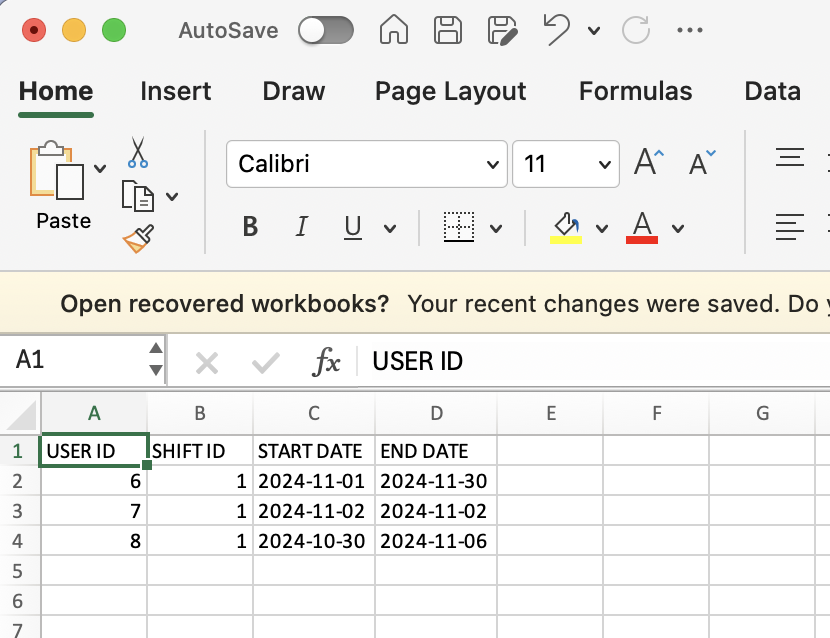
\includegraphics[width=8cm]{Gambar/bab3/user-manual/user-manual-file-excel-shift-scheduling.png}
    	\caption{\textit{File Excel} \textit{Shift Scheduling}}
    	\label{fig:user-manual-file-excel-shift-scheduling}
        \end{figure}
        \FloatBarrier
    \end{enumerate}

    \item Melakukan \textit{Import} Penjadwalan \textit{Shift}
    \begin{enumerate}
        \item Membuka halaman \textit{shift scheduling} yang terdapat pada \textbf{Manual \ref{item:mengakses-shift-scheduling}}.
        \item Menekan tombol "\textit{Import Schedule}" pada halaman \textit{shift scheduling}. \textbf{\ref{fig:user-manual-tombol-import-shift-scheduling}} menunjukkan tombol \textit{"Import Schedule"}.
        \begin{figure}[!htbp]
    	\centering
    	
\includegraphics[width=8cm]{Gambar/bab3/user-manual/user-manual-tombol-import-shift-scheduling.png}
    	\caption{Tombol \textit{Import Shift Scheduling}}
    	\label{fig:user-manual-tombol-import-shift-scheduling}
        \end{figure}
        \FloatBarrier
        \item Meng-\textit{upload} dan mengubah isi \textit{file Excel} yang telah diunduh dari \textbf{Manual \ref{item:export-shift-scheduling}}, kemudian tekan tombol "\textit{Import Now}" untuk me-\textit{replace} seluruh \textit{shift scheduling}. \textbf{\ref{fig:user-manual-modal-import-shift-scheduling}} menunjukkan modal \textit{import shift scheduling}.
        \begin{figure}[!htbp]
    	\centering
    	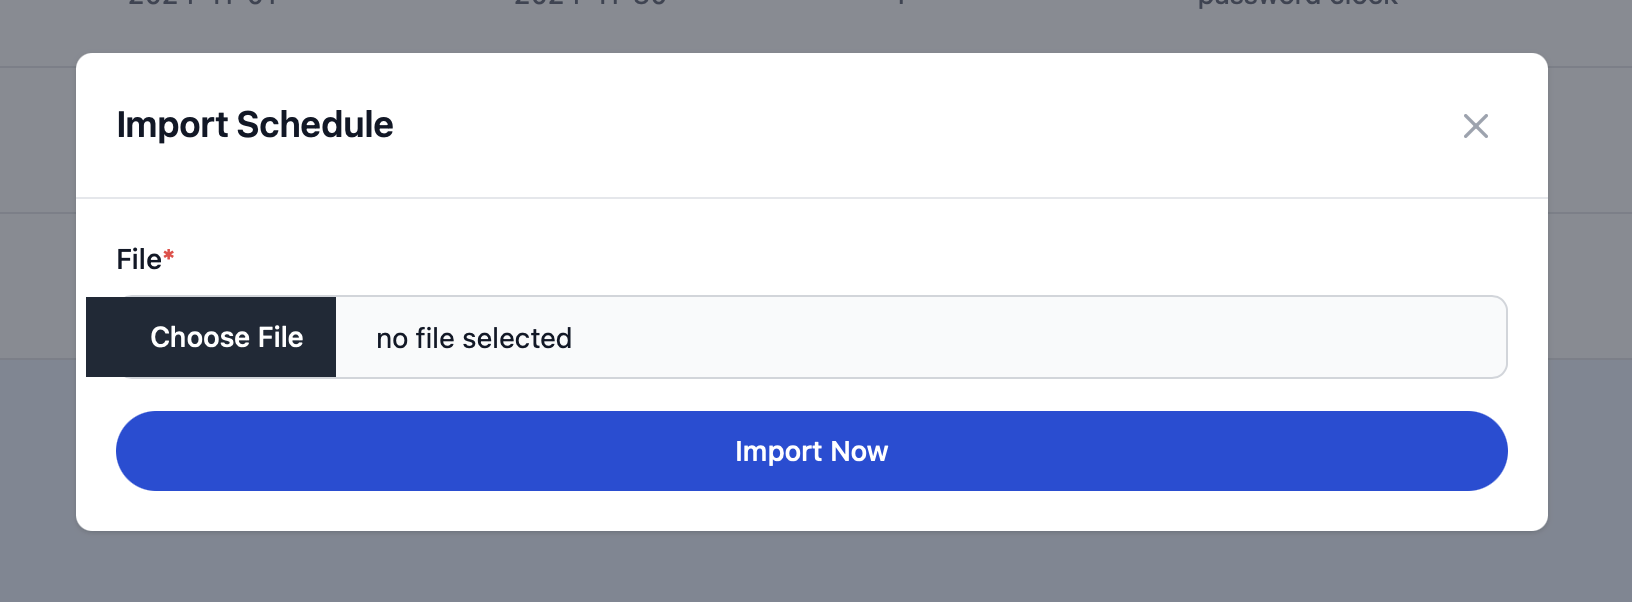
\includegraphics[width=8cm]{Gambar/bab3/user-manual/user-manual-modal-import-shift-scheduling.png}
    	\caption{Modal \textit{Import Shift Scheduling}}
    	\label{fig:user-manual-modal-import-shift-scheduling}
        \end{figure}
        \FloatBarrier
    \end{enumerate}


    \item Mengakses Halaman Jenis Libur Perusahaan\label{item:mengakses-jenis-libur-perusahaan}
    \begin{enumerate}
        \item Melakukan \textit{login} pada aplikasi presensi \textit{online} yang terdapat pada \textbf{Manual \ref{item:melakukan-login}}.
        \item Menekan tombol "\textit{Holiday}" pada \textit{navigation bar} yang terletak di paling atas. \textbf{\ref{fig:user-manual-tombol-holiday-navigation-bar}} menunjukkan tombol \textit{"Holiday"} pada \textit{navigation bar}.
        \begin{figure}[!htbp]
    	\centering
    	
\includegraphics[width=8cm]{Gambar/bab3/user-manual/user-manual-navbar-holiday.png}
    	\caption{Tombol \textit{Holiday} Pada \textit{Navigation Bar}}
    	\label{fig:user-manual-tombol-holiday-navigation-bar}
        \end{figure}
        \FloatBarrier
        \item Sistem akan menampilkan data jenis libur perusahaan pada halaman \textit{holiday}. \textbf{\ref{fig:user-manual-halaman-holiday}} menunjukkan halaman \textit{holiday}.
        \begin{figure}[!htbp]
    	\centering
    	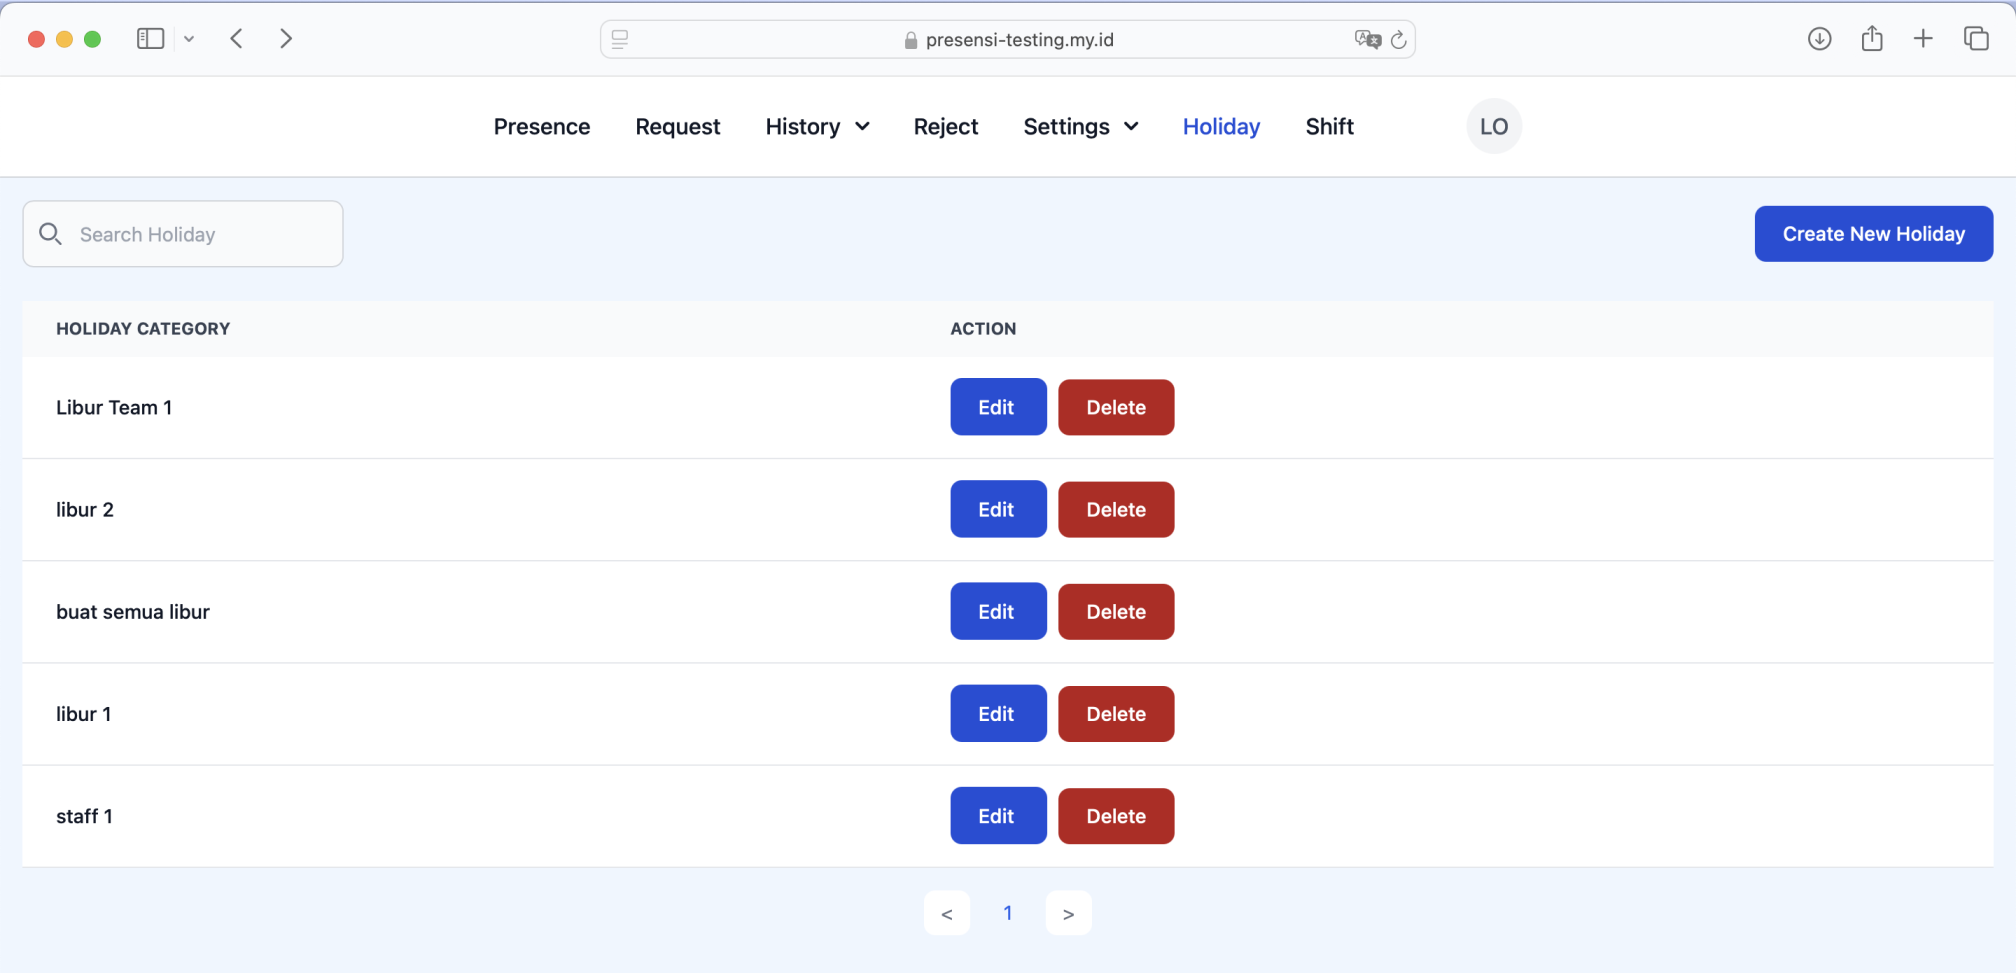
\includegraphics[width=8cm]{Gambar/bab3/user-manual/user-manual-halaman-jenis-libur-perusahaan.png}
    	\caption{Halaman \textit{Holiday}}
    	\label{fig:user-manual-halaman-holiday}
        \end{figure}
        \FloatBarrier
    \end{enumerate}

    \item Menambah Jenis Libur Perusahaan
    \begin{enumerate}
        \item Membuka halaman jenis libur perusahaan yang terdapat pada \textbf{Manual \ref{item:mengakses-jenis-libur-perusahaan}}.
        \item Menekan tombol "\textit{Create New Holiday}" pada halaman \textit{holiday}. \textbf{\ref{fig:user-manual-tombol-create-new-holiday}} menunjukkan tombol "\textit{Create New Holiday}" pada halaman \textit{holiday}.
        \begin{figure}[!htbp]
    	\centering
    	
\includegraphics[width=8cm]{Gambar/bab3/user-manual/user-manual-tombol-create-new-holiday.png}
    	\caption{Tombol "\textit{Create New Holiday}"}
    	\label{fig:user-manual-tombol-create-new-holiday}
        \end{figure}
        \FloatBarrier

        \item Mengisi seluruh \textit{input form} pada modal \textit{create new holiday}, kemudian tekan tombol "\textit{Create New Holiday Category}" untuk menyimpan data jenis libur perusahaan baru. \textbf{\ref{fig:user-manual-modal-create-new-holiday}} menunjukkan modal \textit{create new holiday}.
        \begin{figure}[!htbp]
    	\centering
    	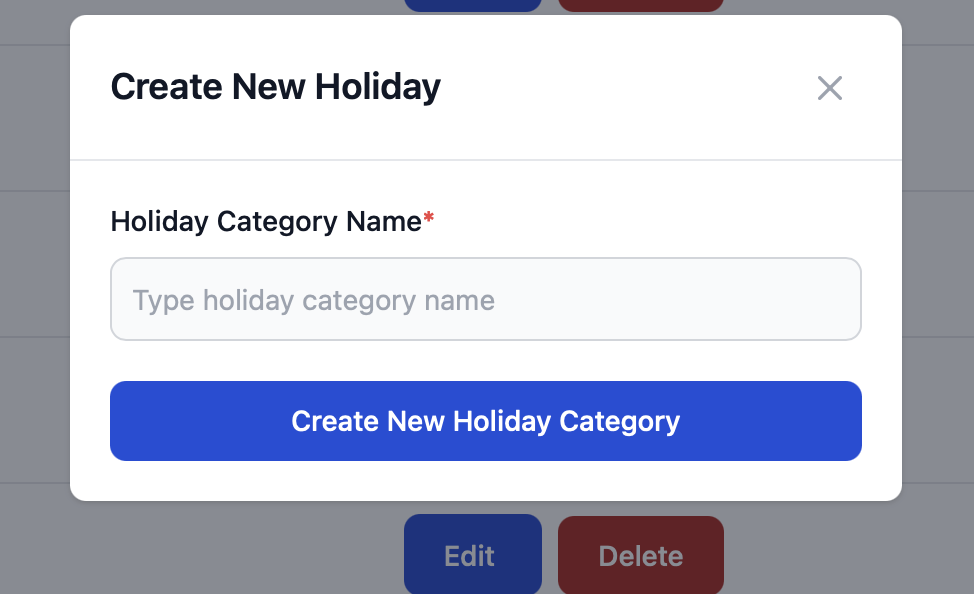
\includegraphics[width=8cm]{Gambar/bab3/user-manual/user-manual-modal-create-new-holiday.png}
    	\caption{Modal \textit{Create New Holiday}}
    	\label{fig:user-manual-modal-create-new-holiday}
        \end{figure}
        \FloatBarrier
    \end{enumerate}

    \item Menghapus Data Jenis Libur Perusahaan
    \begin{enumerate}
        \item Membuka halaman jenis libur perusahaan yang terdapat pada \textbf{Manual \ref{item:mengakses-jenis-libur-perusahaan}}.
        \item Menekan tombol "\textit{Delete}" pada salah satu data \textit{holiday} dan lakukan konfirmasi penghapusan. \textbf{\ref{fig:user-manual-tombol-delete-holiday}} menunjukkan tombol "\textit{Delete}" untuk menghapus data \textit{holiday}.
        \begin{figure}[!htbp]
    	\centering
    	
\includegraphics[width=8cm]{Gambar/bab3/user-manual/user-manual-tombol-delete-holiday.png}
    	\caption{Tombol \textit{Delete Holiday}}
    	\label{fig:user-manual-tombol-delete-holiday}
        \end{figure}
        \FloatBarrier
    \end{enumerate}

    \item Mengakses Halaman Hari Pada Jenis Libur Perusahaan\label{item:mengakses-halaman-hari-jenis-libur-perusahaan}
    \begin{enumerate}
        \item Membuka halaman jenis libur perusahaan yang terdapat pada \textbf{Manual \ref{item:mengakses-jenis-libur-perusahaan}}.
        \item Menekan tombol "\textit{Edit}" salah satu data \textit{holiday} pada halaman \textit{holiday}. \textbf{\ref{fig:user-manual-tombol-edit-holiday}} menunjukkan tombol "\textit{Edit}" pada halaman \textit{holiday}.
        \begin{figure}[!htbp]
    	\centering
    	
\includegraphics[width=8cm]{Gambar/bab3/user-manual/user-manual-tombol-edit-holiday.png}
    	\caption{Tombol \textit{Edit} \textit{Holiday}}
    	\label{fig:user-manual-tombol-edit-holiday}
        \end{figure}
        \FloatBarrier

        \item Sistem akan menampilkan halaman data hari pada jenis perusahaan yang dipilih. \textbf{\ref{fig:user-manual-halaman-hari-jenis-libur-perusahaan}} menunjukkan halaman hari pada jenis libur perusahaan.
        \begin{figure}[!htbp]
    	\centering
    	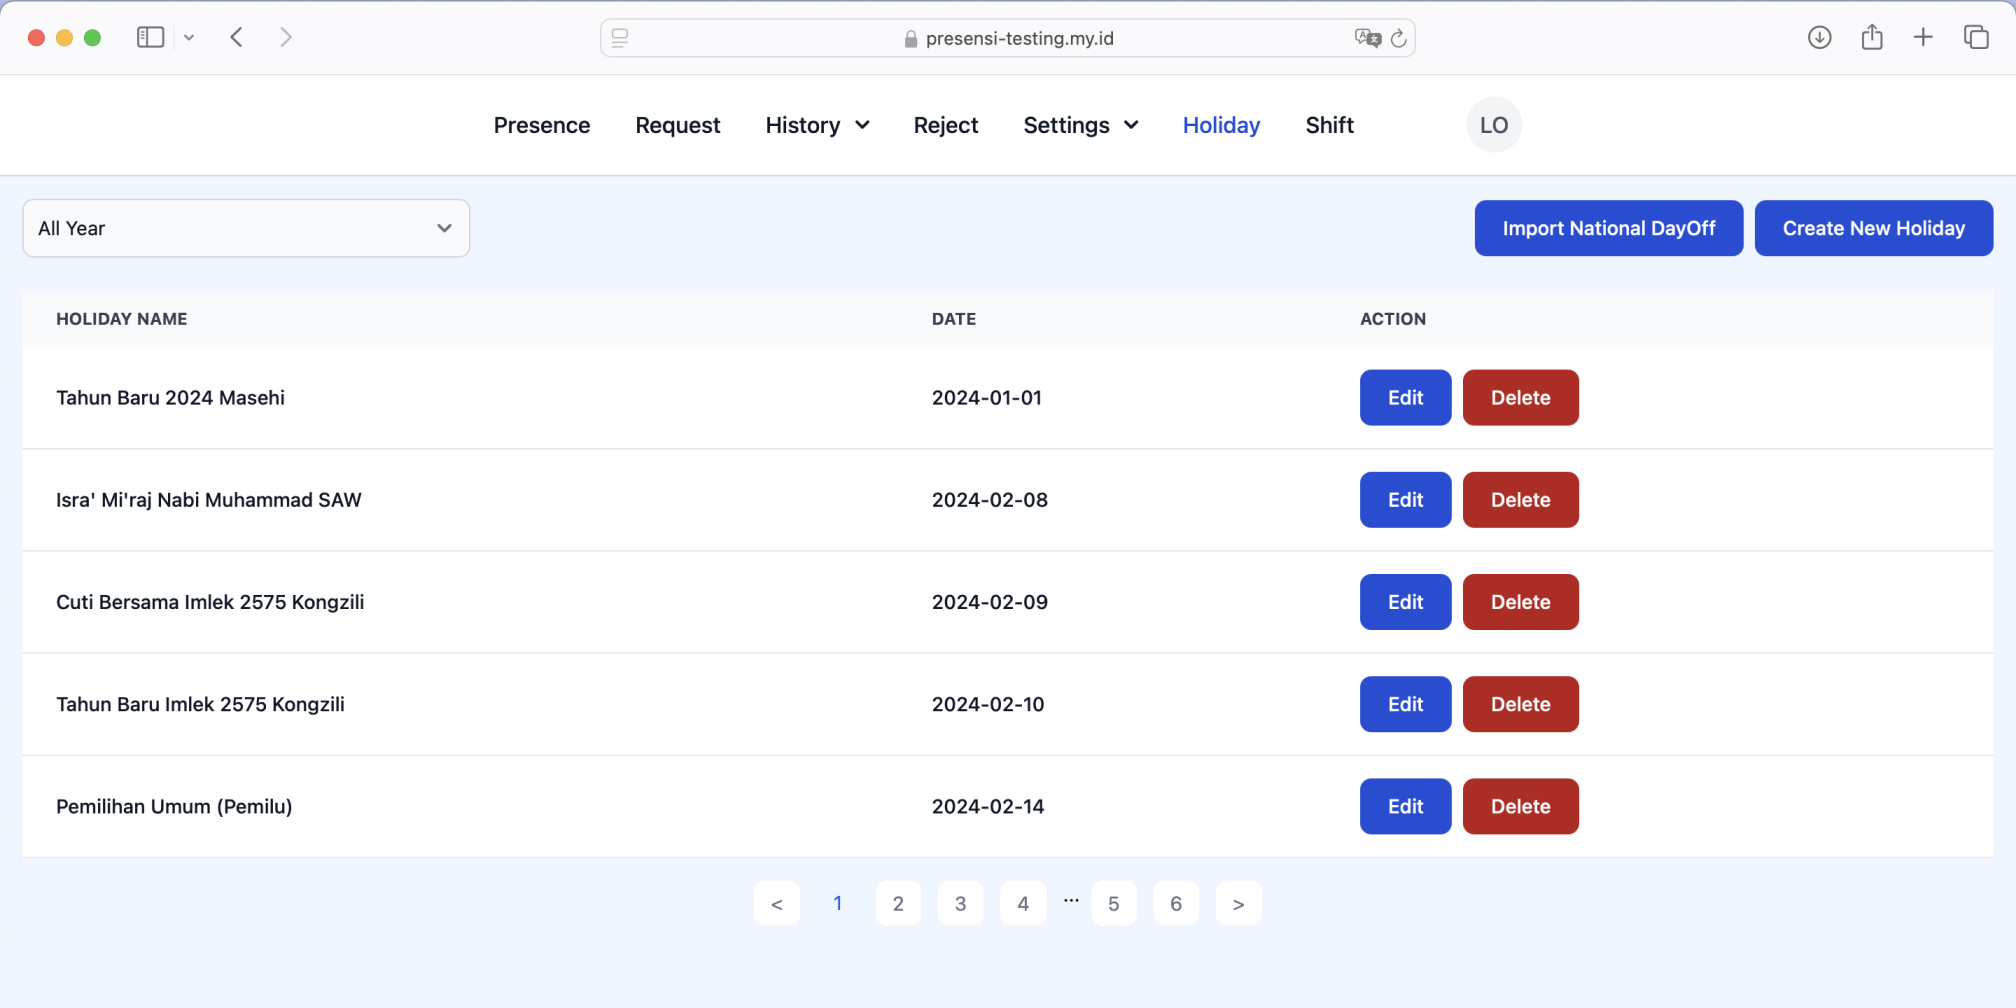
\includegraphics[width=8cm]{Gambar/bab3/user-manual/user-manual-halaman-hari-jenis-libur-perusahaan.png}
    	\caption{Halaman Hari Pada Jenis Libur Perusahaan}
    	\label{fig:user-manual-halaman-hari-jenis-libur-perusahaan}
        \end{figure}
        \FloatBarrier
    \end{enumerate}

    \item Menambah Hari Pada Jenis Libur Perusahaan
    \begin{enumerate}
        \item Membuka halaman pengaturan \textit{department} yang terdapat pada \textbf{Manual \ref{item:mengakses-halaman-hari-jenis-libur-perusahaan}}.
        \item Menekan tombol "\textit{Create New Holiday}" pada halaman hari pada jenis libur perusahaan. \textbf{\ref{fig:user-manual-tombol-tambah-hari-jenis-libur-perusahaan}} menunjukkan tombol "\textit{Create New Holiday}" pada halaman hari pada jenis libur perusahaan.
        \begin{figure}[!htbp]
    	\centering
    	
\includegraphics[width=8cm]{Gambar/bab3/user-manual/user-manual-tombol-tambah-hari-jenis-libur-perusahaan.png}
    	\caption{Tombol "\textit{Create New Holiday}"}
    	\label{fig:user-manual-tombol-tambah-hari-jenis-libur-perusahaan}
        \end{figure}
        \FloatBarrier

        \item Mengisi seluruh \textit{input form} pada modal \textit{create new holiday}, kemudian tekan tombol "\textit{Create New Holiday Category}" untuk menyimpan data hari pada jenis libur perusahaan. \textbf{\ref{fig:user-manual-modal-tambah-hari-pada-jenis-libur-perusahaan}} menunjukkan modal \textit{create new holiday}.
        \begin{figure}[!htbp]
    	\centering
    	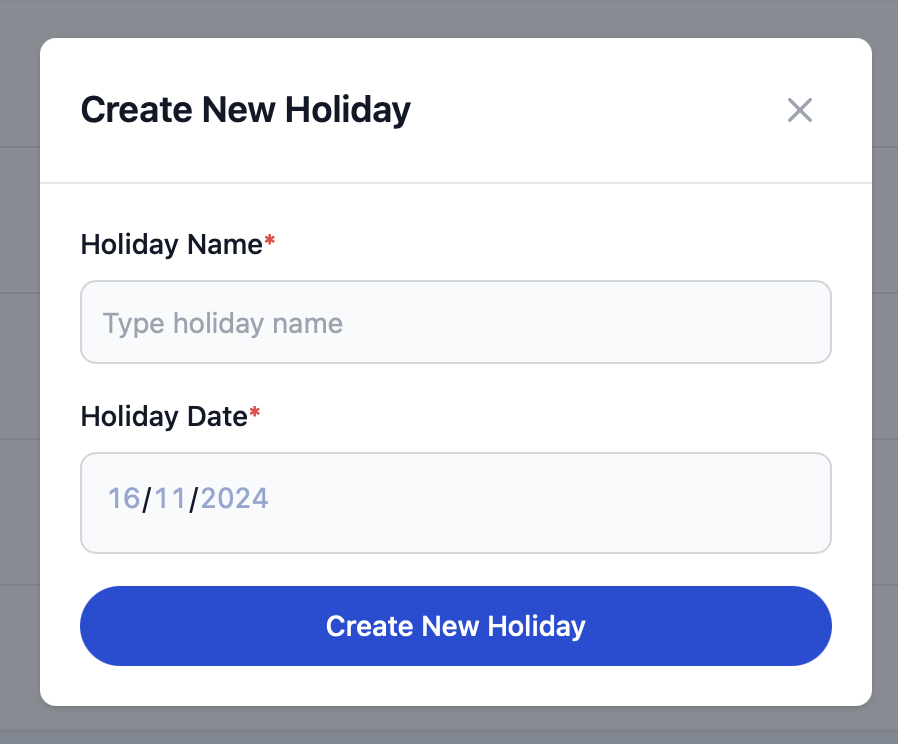
\includegraphics[width=8cm]{Gambar/bab3/user-manual/user-manual-modal-tambah-hari-jenis-libur-perusahaan.png}
    	\caption{Modal \textit{Create New Holiday}}
    	\label{fig:user-manual-modal-tambah-hari-pada-jenis-libur-perusahaan}
        \end{figure}
        \FloatBarrier
    \end{enumerate}


    \item Mengubah Data Hari Pada Jenis Libur Perusahaan
    \begin{enumerate}
        \item Membuka halaman hari pada jenis libur perusahaan yang terdapat pada \textbf{Manual \ref{item:mengakses-halaman-hari-jenis-libur-perusahaan}}.
        \item Menekan tombol "\textit{Edit}" salah satu data hari pada jenis libur perusahaan pada halaman hari jenis libur perusahaan. \textbf{\ref{fig:user-manual-tombol-edit-hari-jenis-libur-perusahaan}} menunjukkan tombol "\textit{Edit}" pada halaman hari jenis libur perusahaan.
        \begin{figure}[!htbp]
    	\centering
    	
\includegraphics[width=8cm]{Gambar/bab3/user-manual/user-manual-tombol-edit-hari-jenis-libur-perusahaan.png}
    	\caption{Tombol \textit{Edit} Pada Jenis Libur Perusahaan}
    	\label{fig:user-manual-tombol-edit-hari-jenis-libur-perusahaan}
        \end{figure}
        \FloatBarrier

        \item Mengubah seluruh \textit{input form} pada modal \textit{edit} hari jenis libur perusahaan, kemudian tekan tombol "\textit{Save Changes}" untuk menyimpan data hari pada jenis libur perusahaan. \textbf{\ref{fig:user-manual-modal-edit-hari-jenis-libur-perusahaan}} menunjukkan modal \textit{edit} hari jenis libur perusahaan.
        \begin{figure}[!htbp]
    	\centering
    	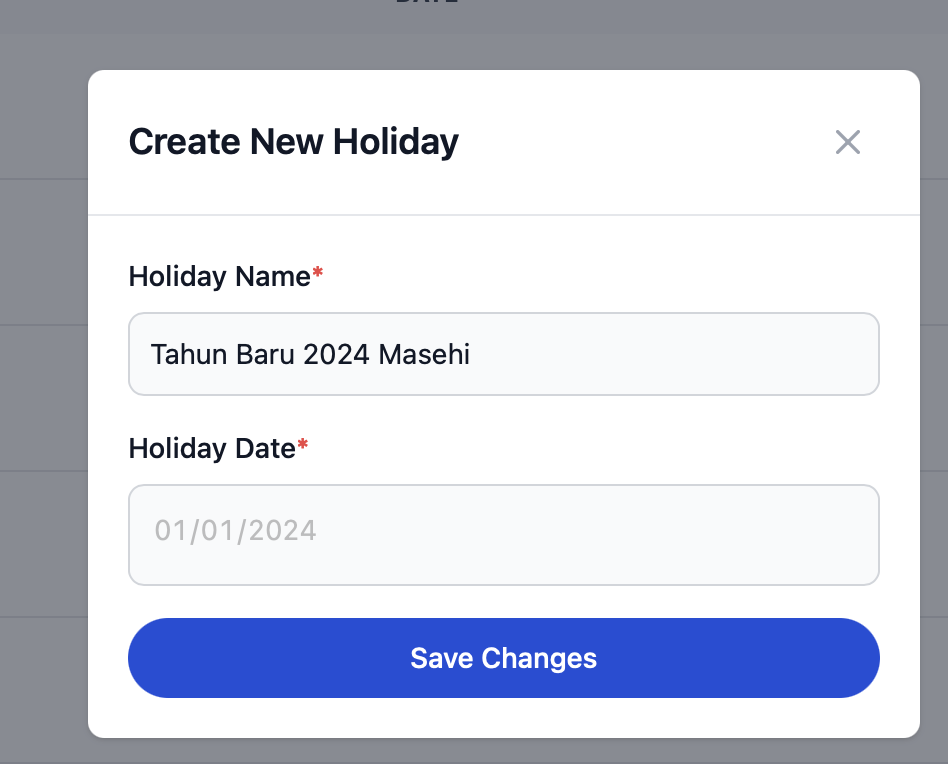
\includegraphics[width=8cm]{Gambar/bab3/user-manual/user-manual-modal-edit-hari-jenis-libur-perusahaan.png}
    	\caption{Modal \textit{Edit} Hari Pada Jenis Libur Perusahaan}
    	\label{fig:user-manual-modal-edit-hari-jenis-libur-perusahaan}
        \end{figure}
        \FloatBarrier
    \end{enumerate}

    \item Menghapus Data Hari Pada Jenis Libur Perusahaan
    \begin{enumerate}
        \item Membuka halaman hari pada jenis libur perusahaan yang terdapat pada \textbf{Manual \ref{item:mengakses-halaman-hari-jenis-libur-perusahaan}}.
        \item Menekan tombol "\textit{Delete}" pada salah satu data hari pada jenis libur perusahaan dan lakukan konfirmasi penghapusan. \textbf{\ref{fig:user-manual-tombol-delete-hari-jenis-libur-perusahaan}} menunjukkan tombol "\textit{Delete}" untuk menghapus data hari pada jenis libur perusahaan.
        \begin{figure}[!htbp]
    	\centering
    	
\includegraphics[width=8cm]{Gambar/bab3/user-manual/user-manual-hapus-hari-jenis-libur-perusahaan.png}
    	\caption{Tombol \textit{Delete} Hari Pada Jenis Libur Perusahaan}
    	\label{fig:user-manual-tombol-delete-hari-jenis-libur-perusahaan}
        \end{figure}
        \FloatBarrier
    \end{enumerate}

    \item Mengimpor Hari Libur Nasional Otomatis Pada Jenis Libur Perusahaan
    \begin{enumerate}
        \item Membuka halaman hari pada jenis libur perusahaan yang terdapat pada \textbf{Manual \ref{item:mengakses-halaman-hari-jenis-libur-perusahaan}}.
        \item Menekan tombol "\textit{Import National DayOff}" pada halaman hari jenis libur perusahaan. \textbf{\ref{fig:user-manual-tombol-import-libur-nasional-hari-jenis-libur-perusahaan}} menunjukkan tombol "\textit{Import National DayOff}" untuk mengambil data libur nasional Indonesia secara otomatis.
        \begin{figure}[!htbp]
    	\centering
    	
\includegraphics[width=8cm]{Gambar/bab3/user-manual/user-manual-tombol-import-hari-libur-nasional.png}
    	\caption{Tombol \textit{Import} Hari Libur Nasional Pada Jenis Libur Perusahaan}
    	\label{fig:user-manual-tombol-import-libur-nasional-hari-jenis-libur-perusahaan}
        \end{figure}
        \FloatBarrier
        \item Memilih tahun yang akan dicari hari liburnya dan menekan tombol "\textit{Add}" untuk melihat \textit{preview} data libur nasional Indonesia, pilih data yang ingin dimasukkan kemudian tekan tombol "\textit{Import Now}" pada modal \textit{import national DayOff}. \textbf{\ref{fig:user-manual-modal-import-libur-nasional-hari-jenis-libur-perusahaan}} menunjukkan modal \textit{import national DayOff}.
        \begin{figure}[!htbp]
    	\centering
    	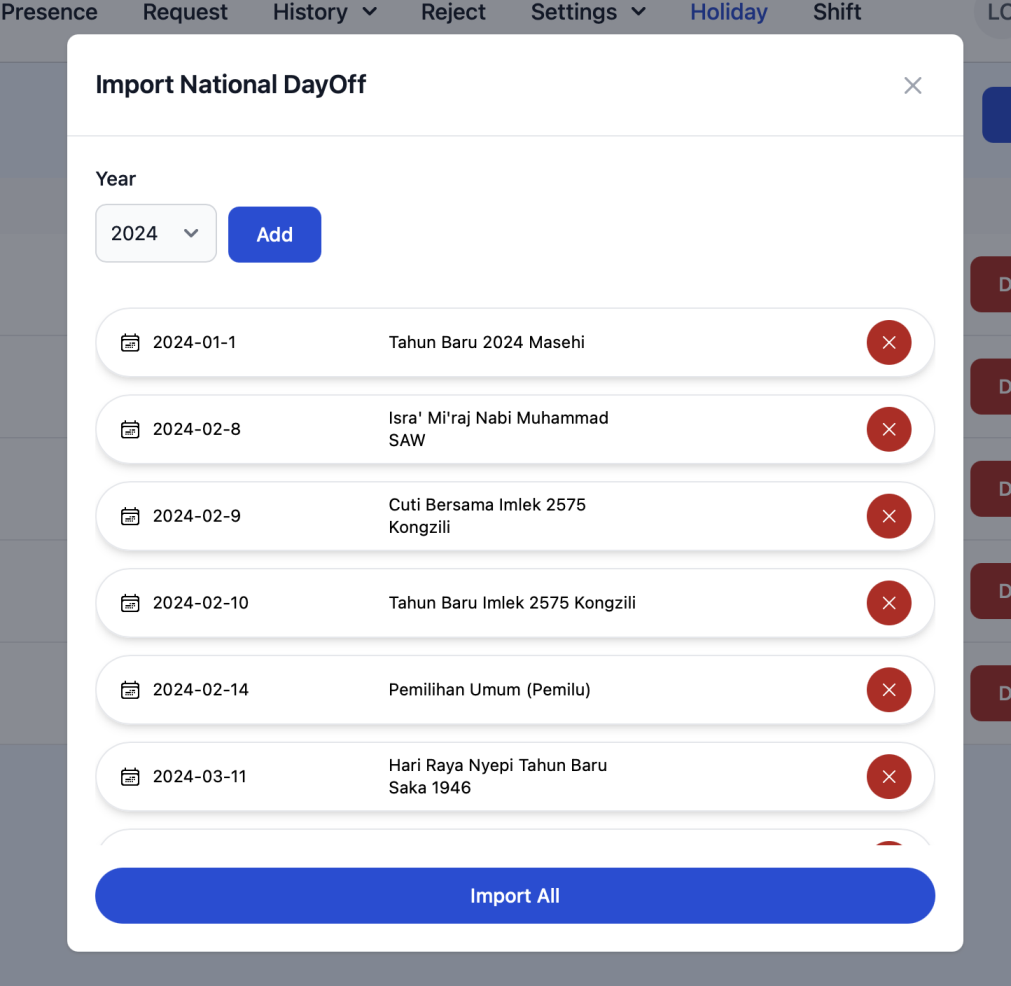
\includegraphics[width=8cm]{Gambar/bab3/user-manual/user-manual-modal-import-hari-libur-nasional.png}
    	\caption{Modal \textit{Import} Hari Libur Nasional Pada Jenis Libur Perusahaan}
    	\label{fig:user-manual-modal-import-libur-nasional-hari-jenis-libur-perusahaan}
        \end{figure}
        \FloatBarrier

         \item Sistem akan menampilkan modal untuk memberikan informasi terkait data yang berhasil di\textit{import} dan gagal. \textbf{\ref{fig:user-manual-modal-hasil-import-libur-nasional-hari-jenis-libur-perusahaan}} menunjukkan hasil \textit{import} data hari libur nasional Indonesia.
    \begin{figure}[!htbp]
    	\centering
    	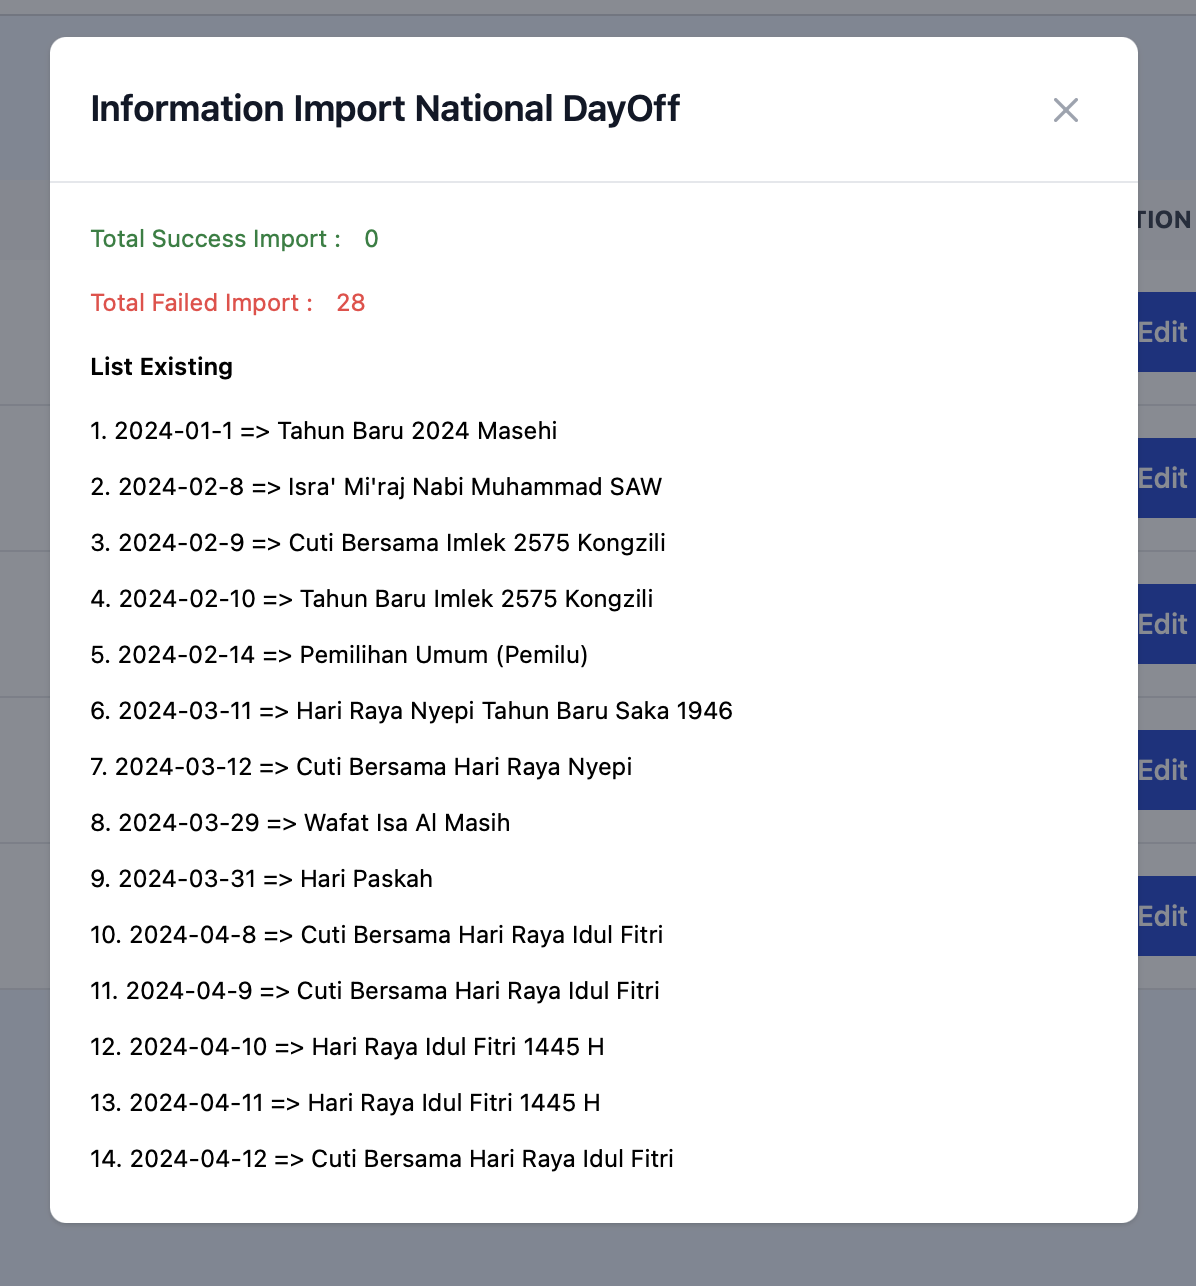
\includegraphics[width=8cm]{Gambar/bab3/user-manual/user-manual-modal-hasil-import-hari-libur-nasional.png}
    	\caption{Modal Hasil \textit{Import} Hari Libur Nasional Pada Jenis Libur Perusahaan}
    	\label{fig:user-manual-modal-hasil-import-libur-nasional-hari-jenis-libur-perusahaan}
        \end{figure}
    \FloatBarrier
    \end{enumerate}

    % BELUM DI INSERT GAMBAR 

    \item Mengakses Halaman Jenis \textit{Shift}\label{item:mengakses-halaman-jenis-shift}
    \begin{enumerate}
        \item Melakukan \textit{login} pada aplikasi presensi \textit{online} yang terdapat pada \textbf{Manual \ref{item:melakukan-login}}.
        \item Menekan tombol "\textit{Shift}" pada \textit{navigation bar} yang terletak di paling atas. \textbf{\ref{fig:user-manual-tombol-shift-pada-navigation-bar}} menunjukkan tombol \textit{"Shift"} pada \textit{navigation bar}.
        \begin{figure}[!htbp]
    	\centering
    	
\includegraphics[width=8cm]{Gambar/bab3/user-manual/user-manual-navbar-shift.png}
    	\caption{Tombol \textit{Shift} Pada \textit{Navigation Bar}}
    	\label{fig:user-manual-tombol-shift-pada-navigation-bar}
        \end{figure}
        \FloatBarrier
        \item Sistem akan menampilkan halaman jenis \textit{shift} beserta data jenis \textit{shift}. \textbf{\ref{fig:user-manual-halaman-jenis-shift}} menunjukkan halaman jenis \textit{shift}.
        \begin{figure}[!htbp]
    	\centering
    	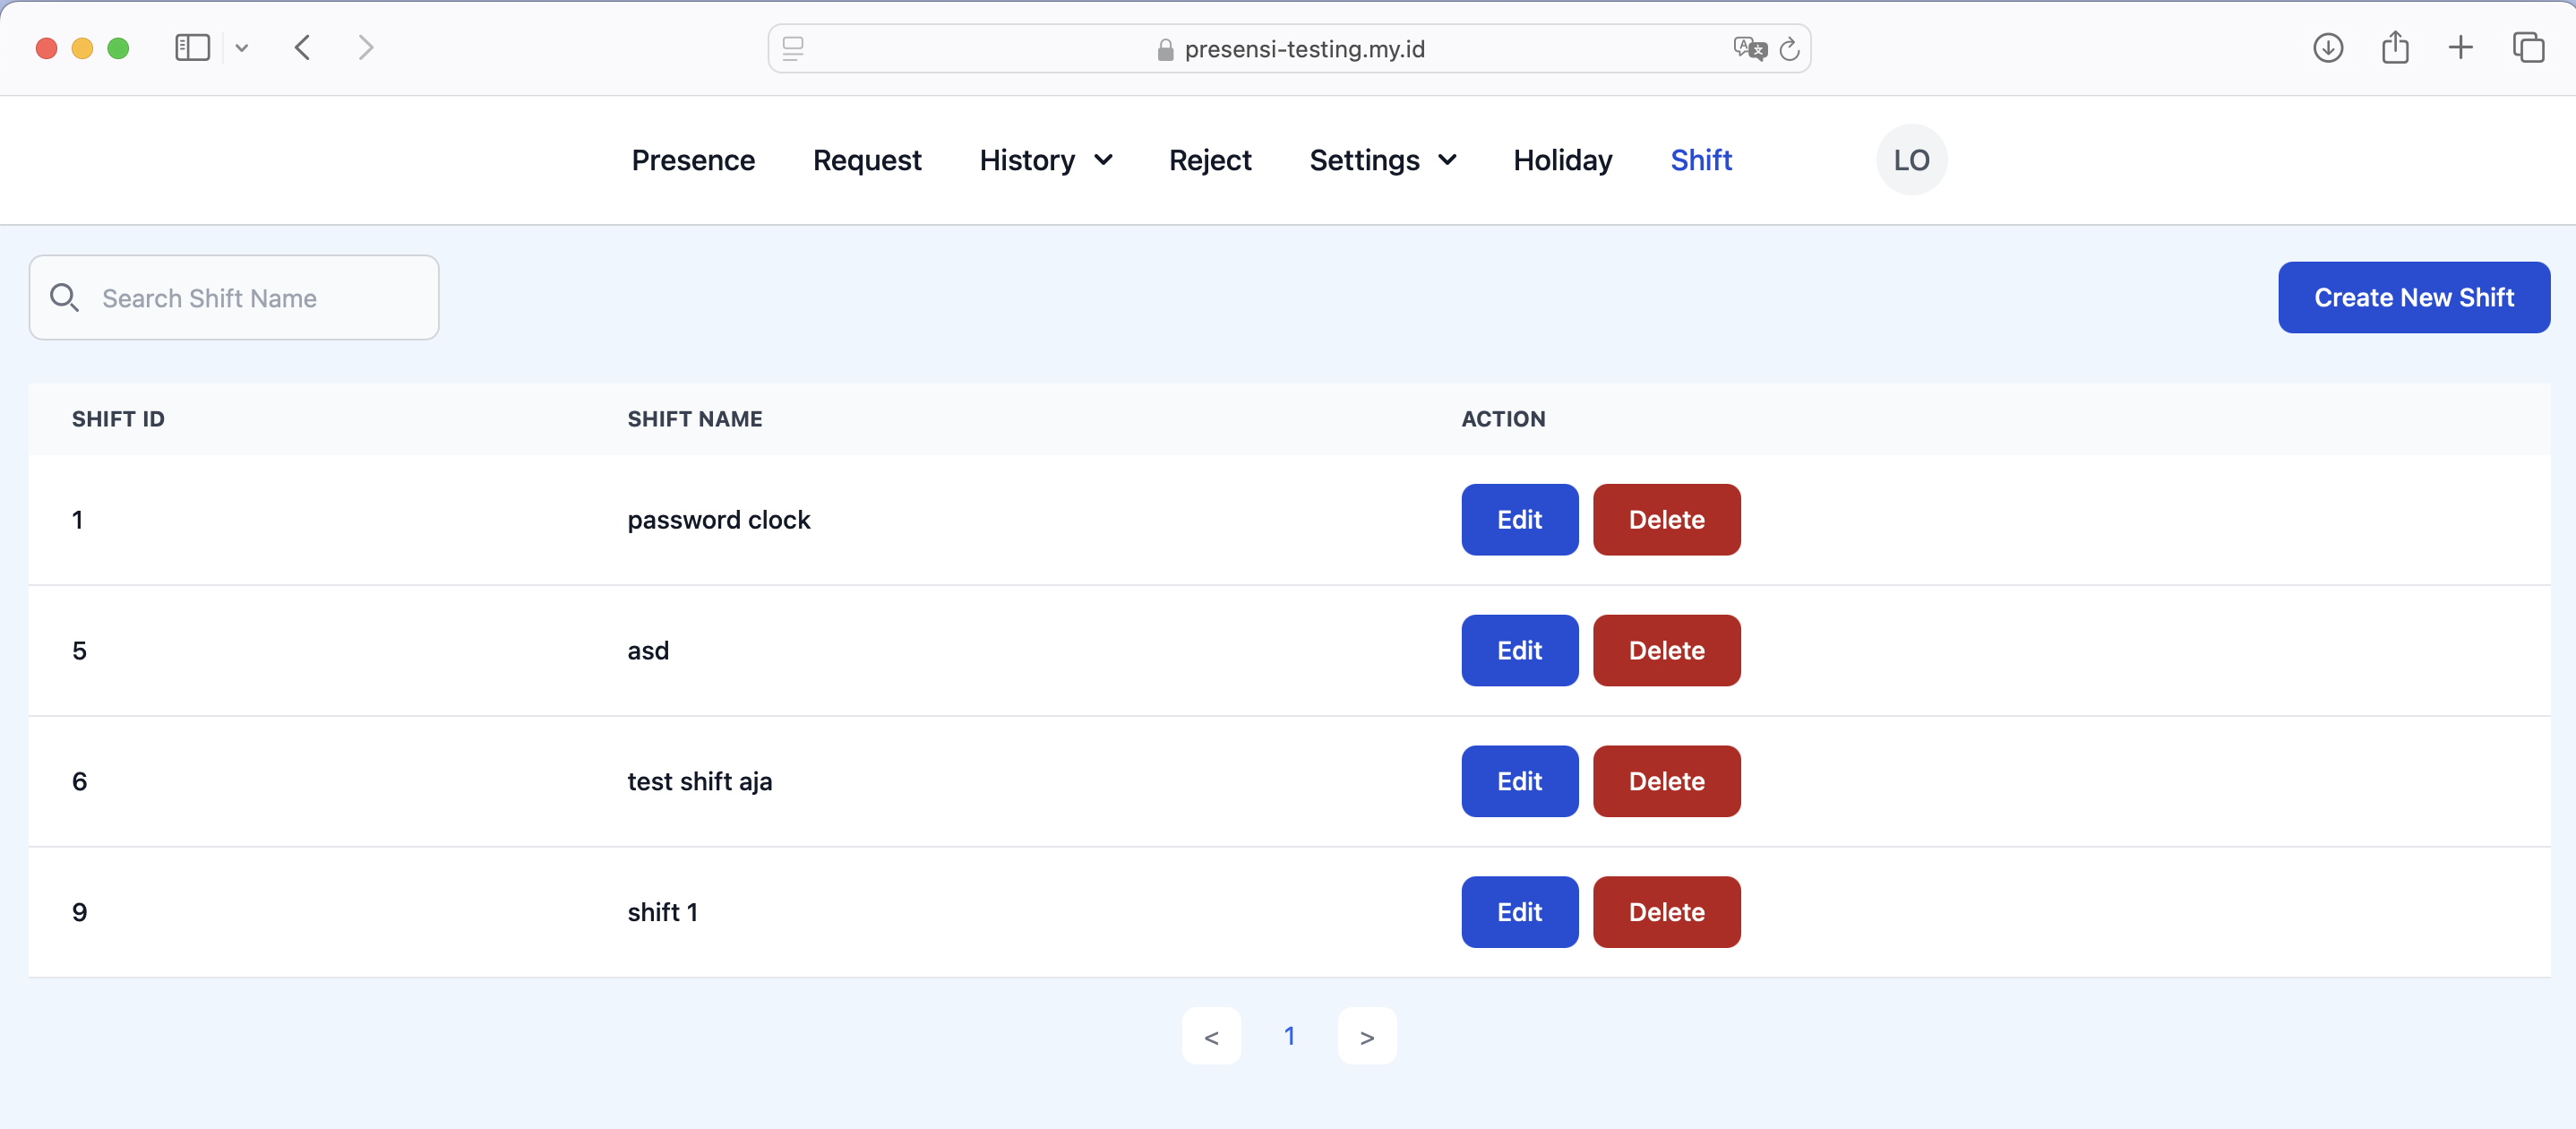
\includegraphics[width=8cm]{Gambar/bab3/user-manual/user-manual-halaman-jenis-shift.png}
    	\caption{Halaman Jenis \textit{Shift}}
    	\label{fig:user-manual-halaman-jenis-shift}
        \end{figure}
        \FloatBarrier
    \end{enumerate}

    \item Menambah Jenis \textit{Shift}
    \begin{enumerate}
        \item Membuka halaman jenis libur \textit{shift} yang terdapat pada \textbf{Manual \ref{item:mengakses-halaman-jenis-shift}}.
        \item Menekan tombol "\textit{Create New Shift}" pada halaman jenis \textit{shift}. \textbf{\ref{fig:user-manual-tombol-create-new-shift}} menunjukkan tombol "\textit{Create New Shift}" pada halaman jenis \textit{shift}.
        \begin{figure}[!htbp]
    	\centering
    	
\includegraphics[width=8cm]{Gambar/bab3/user-manual/user-manual-tombol-create-new-shift.png}
    	\caption{Tombol \textit{Create New Shift} Pada Halaman Jenis \textit{Shift}}
    	\label{fig:user-manual-tombol-create-new-shift}
        \end{figure}
        \FloatBarrier
        \item Mengisi seluruh \textit{input form} pada modal \textit{create new shift} dan tekan tombol \textit{"Create New Shift"} untuk menyimpan data jenis \textit{shift} baru. \textbf{\ref{fig:user-manual-modal-create-new-shift}} menunjukkan modal \textit{create new shift}.
        \begin{figure}[!htbp]
    	\centering
    	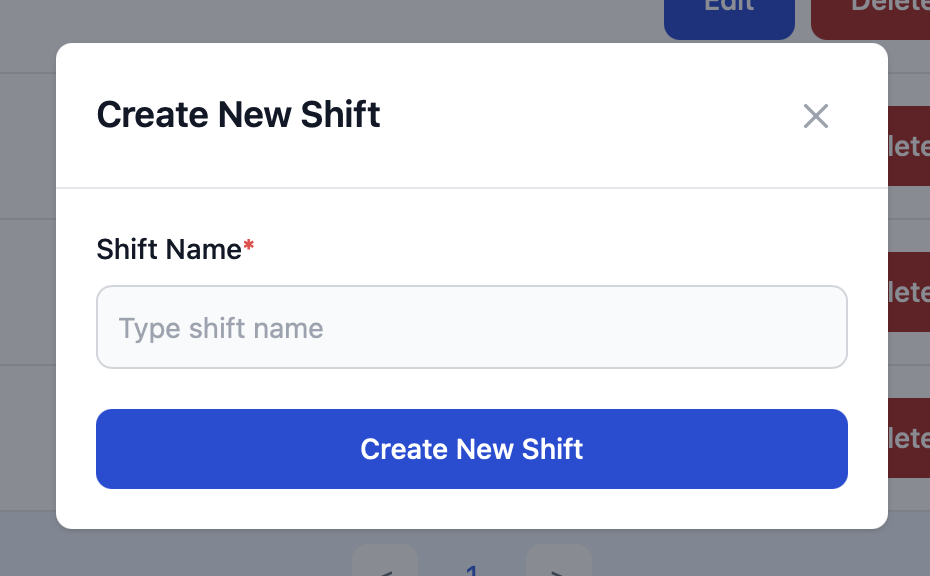
\includegraphics[width=8cm]{Gambar/bab3/user-manual/user-manual-modal-create-new-shift.png}
    	\caption{Modal \textit{Create New Shift} Pada Halaman Jenis \textit{Shift}}
    	\label{fig:user-manual-modal-create-new-shift}
        \end{figure}
        \FloatBarrier
    \end{enumerate}

    \item Menghapus Jenis \textit{Shift}
    \begin{enumerate}
        \item Membuka halaman jenis libur \textit{shift} yang terdapat pada \textbf{Manual \ref{item:mengakses-halaman-jenis-shift}}.
        \item Menekan tombol "\textit{Delete}" pada salah satu data jenis \textit{shift} melalui halaman jenis \textit{shift} dan melakukan konfirmasi. \textbf{\ref{fig:user-manual-tombol-delete-shift}} menunjukkan tombol "\textit{Delete}" pada salah satu data jenis \textit{shift}.
        \begin{figure}[!htbp]
    	\centering
    	
\includegraphics[width=5cm]{Gambar/bab3/user-manual/user-manual-tombol-delete-shift.png}
    	\caption{Tombol \textit{Delete} Pada Jenis \textit{Shift}}
    	\label{fig:user-manual-tombol-delete-shift}
        \end{figure}
        \FloatBarrier
    \end{enumerate}

    \item Melakukan \textit{Edit} Jenis \textit{Shift}\label{item:melakukan-edit-jenis-shift}
    \begin{enumerate}
        \item Membuka halaman jenis libur \textit{shift} yang terdapat pada \textbf{Manual \ref{item:mengakses-halaman-jenis-shift}}.
        \item Menekan tombol "\textit{Edit}" pada salah satu data jenis \textit{shift} melalui halaman jenis \textit{shift}. \textbf{\ref{fig:user-manual-tombol-edit-shift}} menunjukkan tombol "\textit{Edit}" pada salah satu data jenis \textit{shift}.
        \begin{figure}[!htbp]
    	\centering
    	
\includegraphics[width=5cm]{Gambar/bab3/user-manual/user-manual-tombol-edit-shift.png}
    	\caption{Tombol \textit{Edit} Pada Jenis \textit{Shift}}
    	\label{fig:user-manual-tombol-edit-shift}
        \end{figure}
        \FloatBarrier
        
        \item Mengisi \textit{input form} pada modal \textit{edit shift} dan tekan tombol "\textit{Save Changes}" untuk menyimpan perubahan jenis \textit{shift}. \textbf{\ref{fig:user-manual-tombol-edit-jenis-shift}} menunjukkan modal \textit{edit shift}.
        \begin{figure}[!htbp]
    	\centering
    	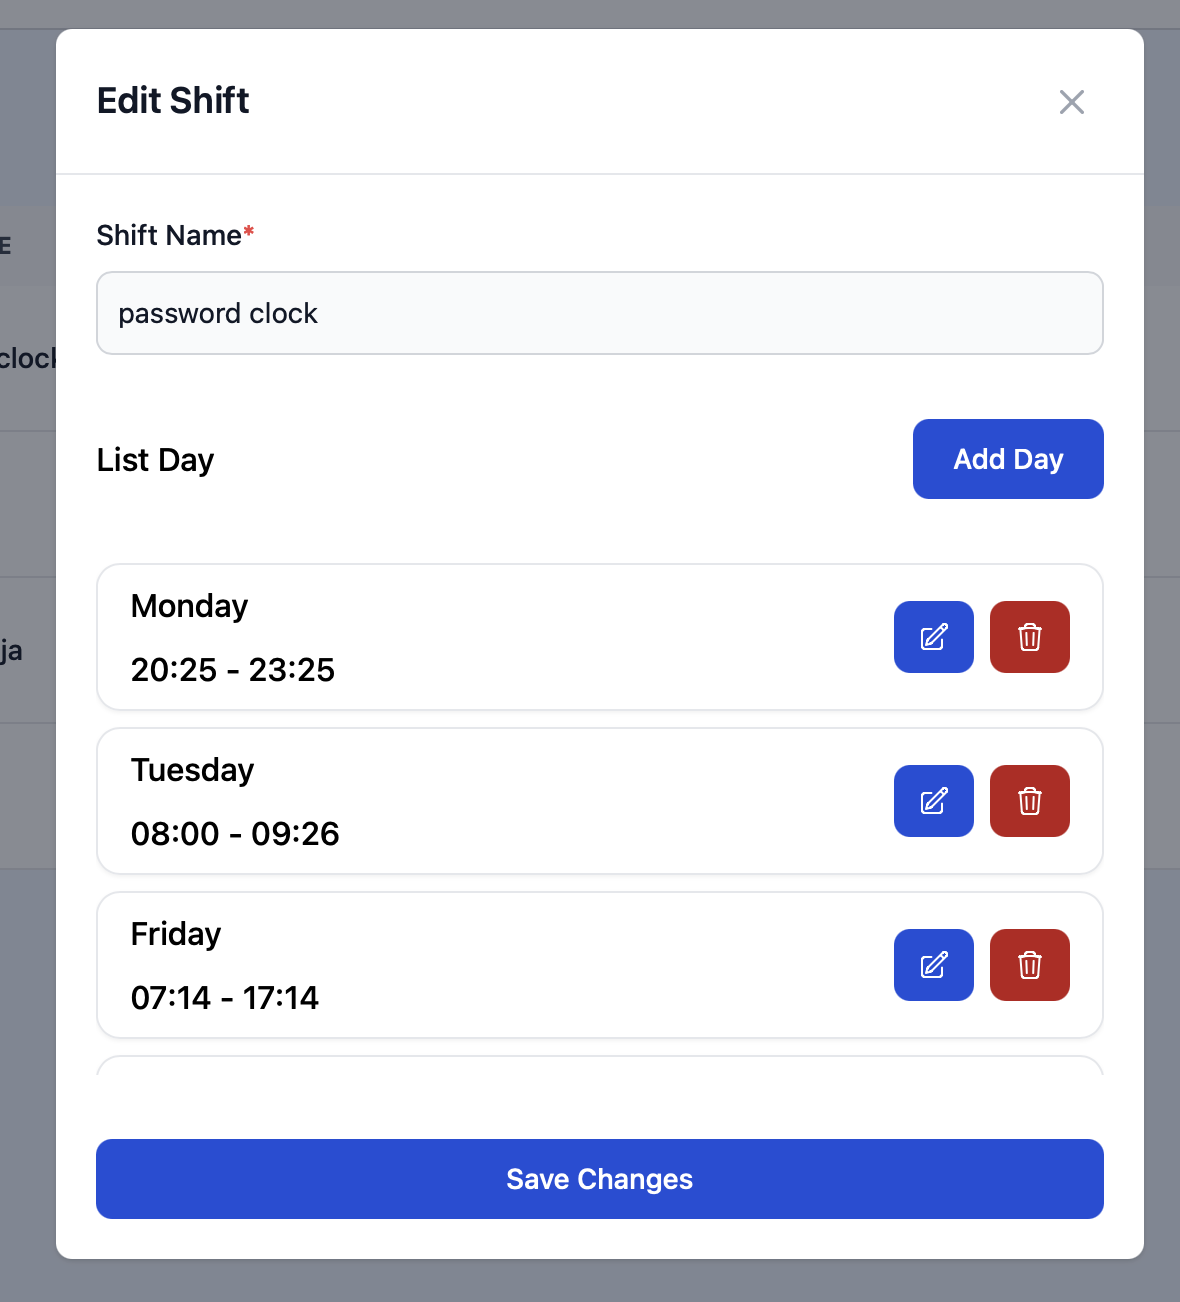
\includegraphics[width=8cm]{Gambar/bab3/user-manual/user-manual-modal-edit-shift.png}
    	\caption{Tombol \textit{Edit} Pada Jenis \textit{Shift}}
    	\label{fig:user-manual-tombol-edit-jenis-shift}
        \end{figure}
        \FloatBarrier
    \end{enumerate}

    \item Menambah Hari Pada Jenis \textit{Shift}
    \begin{enumerate}
        \item Mengakses modal \textit{edit} jenis \textit{shift} pada \textbf{Manual \ref{item:melakukan-edit-jenis-shift}}.
        \item Menekan tombol "\textit{Add Day}" pada modal \textit{edit} jenis \textit{shift}. \textbf{\ref{fig:user-manual-tombol-add-shift-day}} menunjukkan tombol \textit{"Add Day"} untuk membuka modal \textit{add shift day}.
        \begin{figure}[!htbp]
    	\centering
    	
\includegraphics[width=5cm]{Gambar/bab3/user-manual/user-manual-tombol-add-shiftday.png}
    	\caption{Tombol \textit{Add Day} Pada Jenis \textit{Shift}}
    	\label{fig:user-manual-tombol-add-shift-day}
        \end{figure}
        \FloatBarrier
        \item Mengisi seluruh \textit{input form} pada \textit{add shift day} dan menekan tombol "\textit{Add Day}" untuk menyimpan hari baru pada jenis \textit{shift}. \textbf{\ref{fig:user-manual-modal-add-shift-day}} menunjukkan modal \textit{add shift day} untuk menambah hari baru pada jenis \textit{shift}.
        \begin{figure}[!htbp]
    	\centering
    	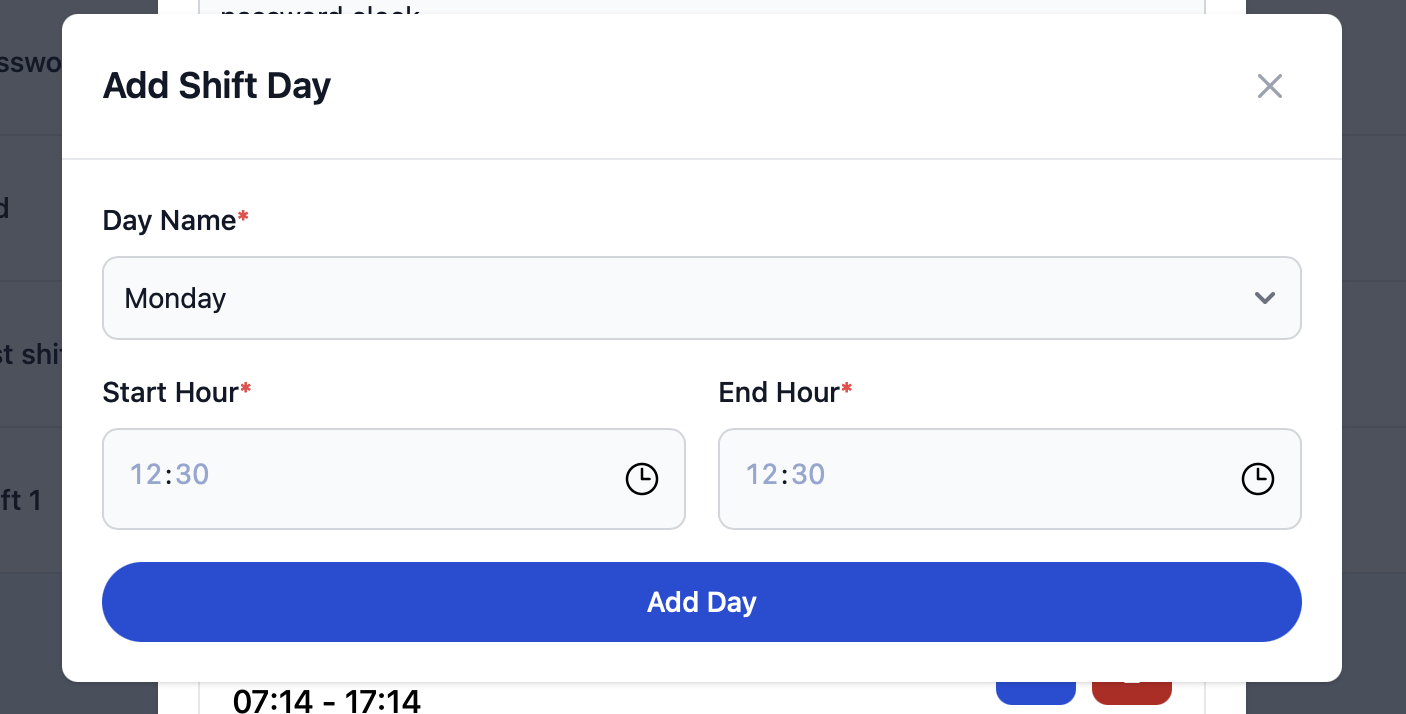
\includegraphics[width=8cm]{Gambar/bab3/user-manual/user-manual-modal-add-shiftday.png}
    	\caption{Modal \textit{Add New Day} Pada Jenis \textit{Shift}}
    	\label{fig:user-manual-modal-add-shift-day}
        \end{figure}
        \FloatBarrier
        
    \end{enumerate}

    \item Melakukan \textit{Edit} Hari Pada Jenis \textit{Shift}
    \begin{enumerate}
        \item Mengakses modal \textit{edit} jenis \textit{shift} pada \textbf{Manual \ref{item:melakukan-edit-jenis-shift}}.
        \item Menekan logo \textit{edit} salah satu hari pada modal \textit{edit} jenis \textit{shift}. \textbf{\ref{fig:user-manual-tombol-edit-shift-day}} menunjukkan tombol logo \textit{edit} untuk mengubah data hari pada jenis \textit{shift}.
        \begin{figure}[!htbp]
    	\centering
    	
\includegraphics[width=5cm]{Gambar/bab3/user-manual/user-manual-tombol-edit-shiftday.png}
    	\caption{Tombol \textit{Edit Day} Pada Jenis \textit{Shift}}
    	\label{fig:user-manual-tombol-edit-shift-day}
        \end{figure}
        \FloatBarrier
        \item Mengubah isi \textit{input form} pada modal \textit{edit shift day} dan menekan tombol \textit{"Edit Day"} untuk menyimpan perubahan data hari pada jenis \textit{shift}. \textbf{\ref{fig:user-manual-modal-edit-shift-day}} menunjukkan modal \textit{edit shift day} untuk mengubah data hari pada jenis \textit{shift}.
        \begin{figure}[!htbp]
    	\centering
    	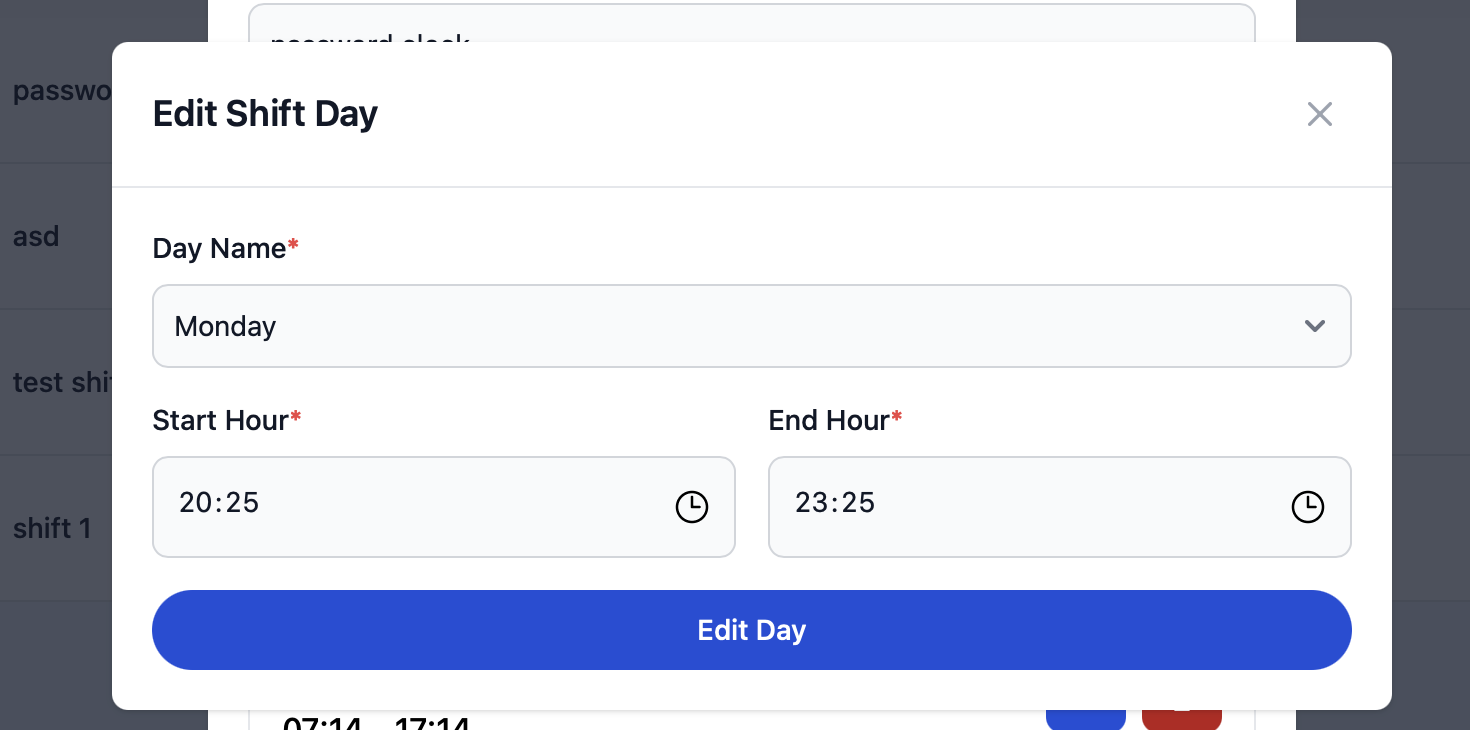
\includegraphics[width=8cm]{Gambar/bab3/user-manual/user-manual-modal-edit-shiftday.png}
    	\caption{Modal \textit{Edit Day} Pada Jenis \textit{Shift}}
    	\label{fig:user-manual-modal-edit-shift-day}
        \end{figure}
        \FloatBarrier
    \end{enumerate}

    \item Menghapus Hari Pada Jenis Shift
    \begin{enumerate}
        \item Mengakses modal \textit{edit} jenis \textit{shift} pada \textbf{Manual \ref{item:melakukan-edit-jenis-shift}}.
        \item Menekan tombol logo hapus salah satu data hari pada modal \textit{edit} jenis \textit{shift} dan melakukan konfirmasi penghapusan. \textbf{\ref{fig:user-manual-tombol-delete-shift-day}} menunjukkan tombol logo hapus salah satu data hari pada jenis \textit{shift}.
        \begin{figure}[!htbp]
    	\centering
    	
\includegraphics[width=5cm]{Gambar/bab3/user-manual/user-manual-tombol-delete-shiftday.png}
    	\caption{Tombol \textit{Delete} Hari Pada Jenis \textit{Shift}}
    	\label{fig:user-manual-tombol-delete-shift-day}
        \end{figure}
        \FloatBarrier
    \end{enumerate}

    \item Melakukan Ganti Kata Sandi Akun
    \begin{enumerate}
        \item Melakukan \textit{login} pada aplikasi presensi \textit{online} yang terdapat pada \textbf{Manual \ref{item:melakukan-login}}.
        \item Menekan ikon profil pada \textit{navigation bar} yang terletak di paling atas, kemudian memilih tombol "\textit{Change Password}". \textbf{\ref{fig:user-manual-tombol-change-password-pada-navigation-bar}} menunjukkan tombol \textit{"Change Password"} pada \textit{navigation bar}.
        \begin{figure}[!htbp]
    	\centering
    	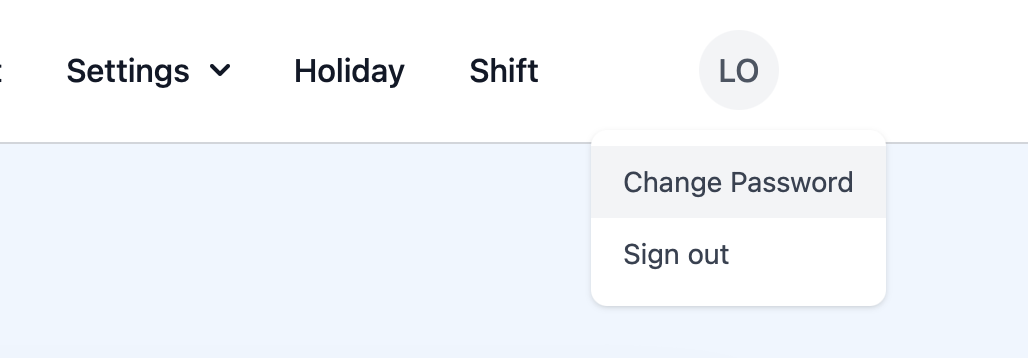
\includegraphics[width=8cm]{Gambar/bab3/user-manual/user-manual-navbar-change-password.png}
    	\caption{Tombol \textit{Change Password} Pada \textit{Navigation Bar}}
    	\label{fig:user-manual-tombol-change-password-pada-navigation-bar}
        \end{figure}
        \FloatBarrier
        \item Mengisi seluruh \textit{input form password} lama dan baru, kemudian tekan tombol "\textit{Submit}" untuk menyimpan perubahan \textit{password} baru pada akun. \textbf{\ref{fig:user-manual-halaman-change-password}} menunjukkan \textit{form} untuk pengubahan \textit{password} akun. 
        \begin{figure}[!htbp]
    	\centering
    	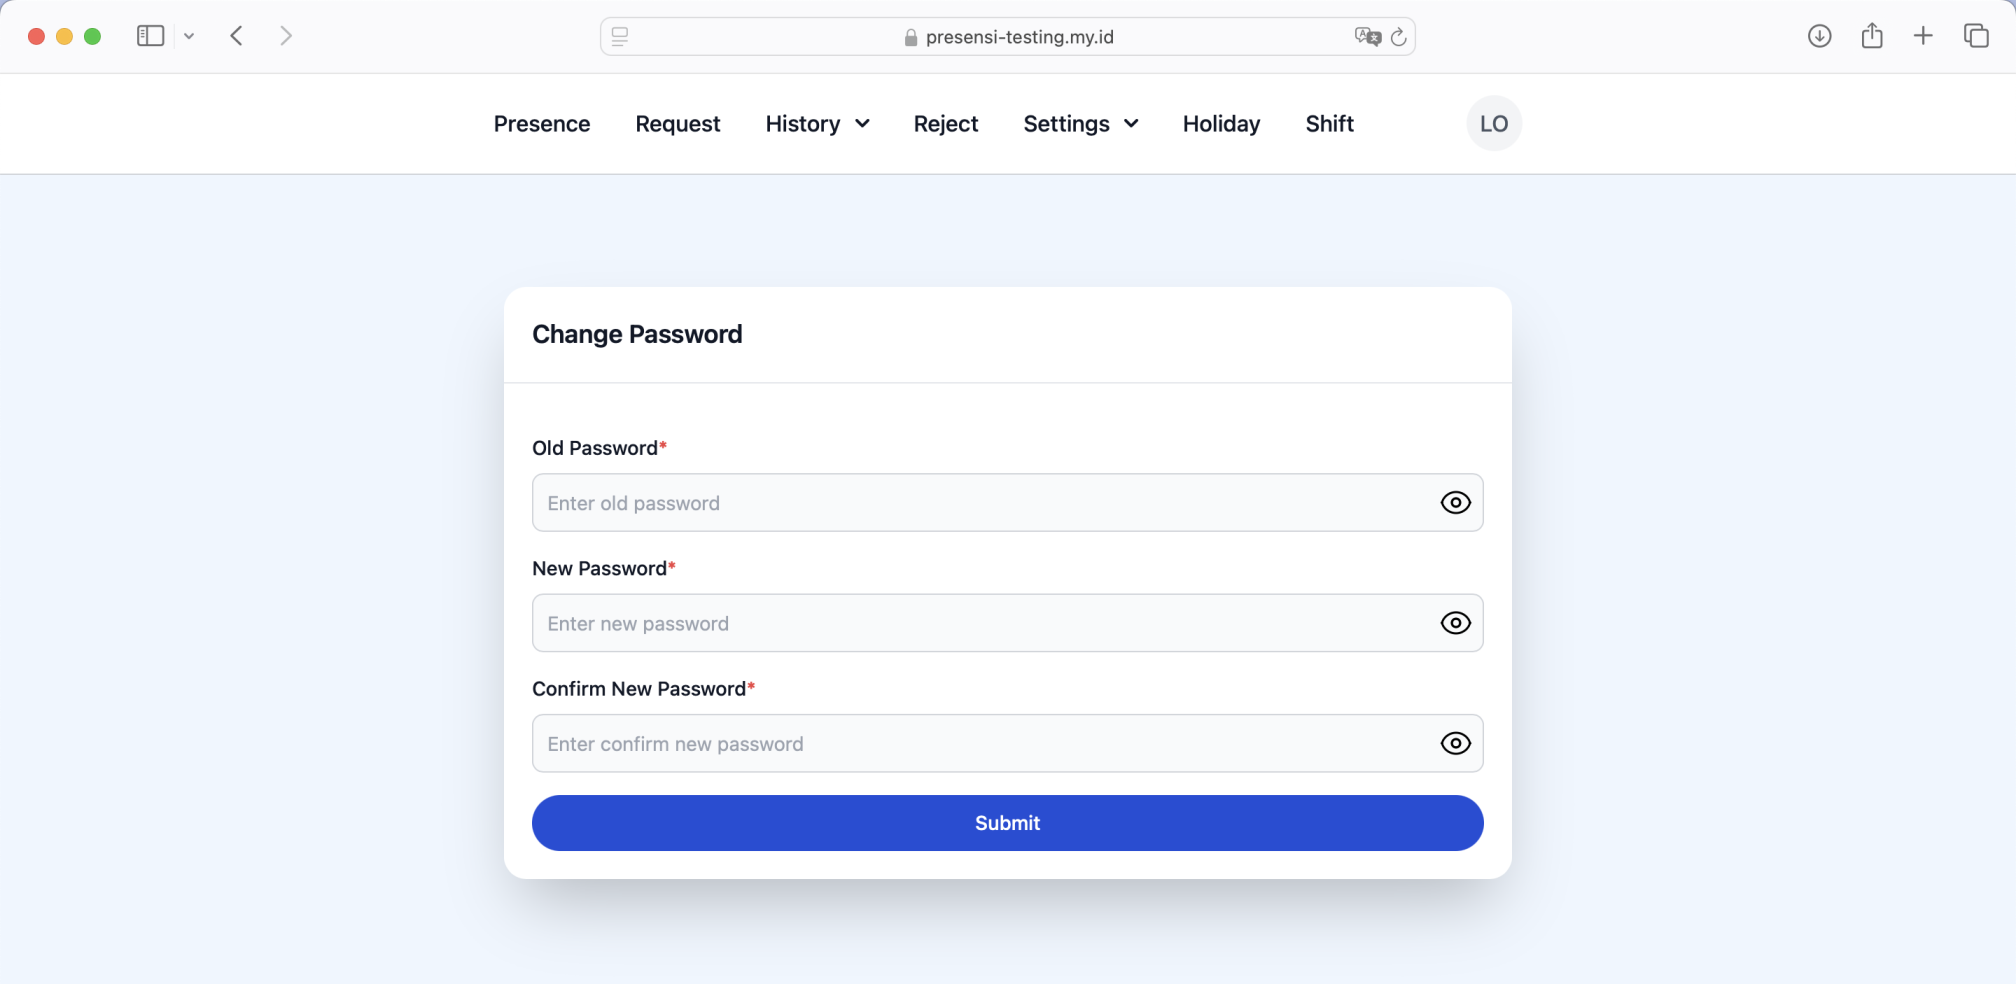
\includegraphics[width=8cm]{Gambar/bab3/user-manual/user-manual-halaman-change-password.png}
    	\caption{Halaman \textit{Change Password}}
    	\label{fig:user-manual-halaman-change-password}
        \end{figure}
        \FloatBarrier
    \end{enumerate}

    \item Melakukan \textit{Logout}
    \begin{enumerate}
        \item Melakukan \textit{login} pada aplikasi presensi \textit{online} yang terdapat pada \textbf{Manual \ref{item:melakukan-login}}.
        \item Menekan ikon profil pada \textit{navigation bar} yang terletak di paling atas, kemudian memilih tombol "\textit{Sign Out}". \textbf{\ref{fig:user-manual-tombol-sign-out-pada-navigation-bar}} menunjukkan tombol \textit{"Sign Out"} pada \textit{navigation bar}.
        \begin{figure}[!htbp]
    	\centering
    	
\includegraphics[width=8cm]{Gambar/bab3/user-manual/user-manual-navbar-sign-out.png}
    	\caption{Tombol \textit{Sign Out} Pada \textit{Navigation Bar}}
    	\label{fig:user-manual-tombol-sign-out-pada-navigation-bar}
        \end{figure}
        \FloatBarrier
        \item Halaman akan dialihkan ke halaman \textit{login}.
    \end{enumerate}
   
\end{enumerate}
\pagebreak

\begin{landscape}
\nextappendix
\section*{Lampiran \theappendixletter: Gantt Chart Implementasi Sistem}
\label{sec:gantt-chart-implementasi-sistem}
\addcontentsline{toc}{section}{Lampiran \theappendixletter: Gantt Chart Implementasi Sistem}
\begin{figure}[H]
	\centering
	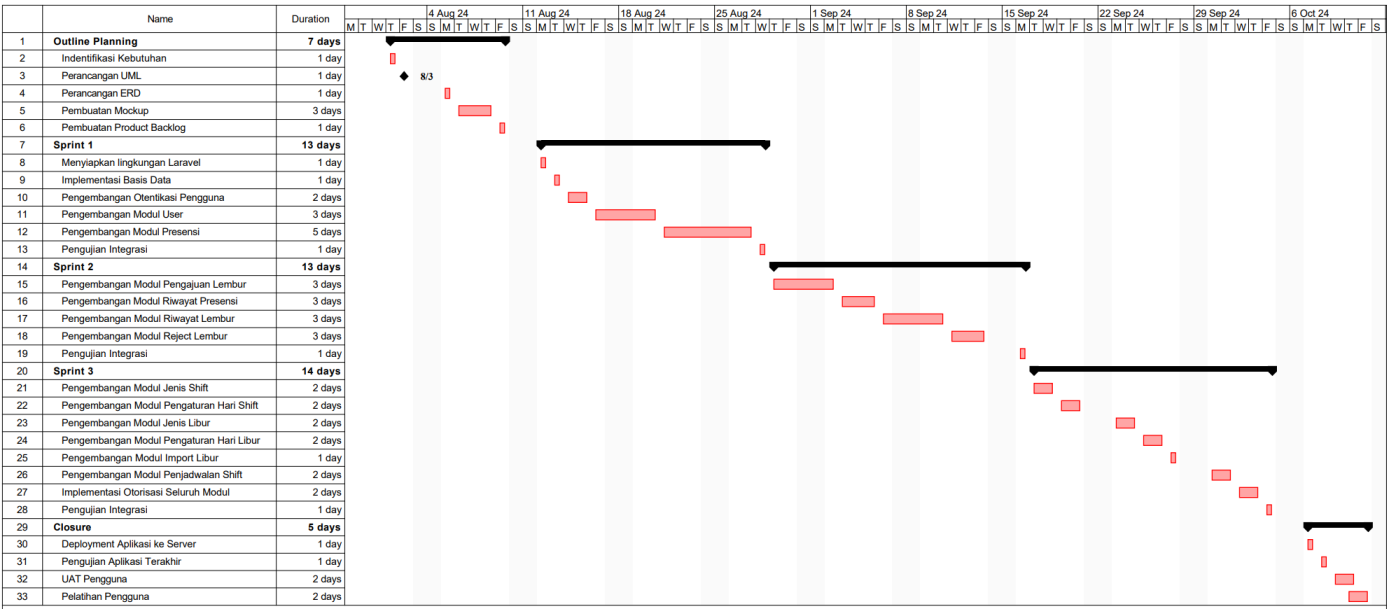
\includegraphics[width=24cm]{Gambar/bab3/gantt-chart.png}
	\caption{Gantt Chart Implementasi Sistem}
	\label{fig:gantt-chart-implementasi-sistem}
\end{figure}
\end{landscape}
\pagebreak

\nextappendix
\section*{Lampiran \theappendixletter: Hasil \textit{Whitebox Testing} Oleh \textit{Programmer}
\label{sec:whitebox-testing-aplikasi-presensi-online-oleh-programmer}}
\addcontentsline{toc}{section}{Lampiran \theappendixletter: Hasil \textit{Whitebox Testing} Oleh \textit{Programmer}}
\begin{longtable}{ |p{3cm}|p{4cm}|p{4cm}|p{2cm}|}
\caption{Hasil \textit{Whitebox Testing} Aplikasi Presensi \textit{Online} Oleh \textit{Programmer}}\label{tab:table-whitebox-testing-aplikasi-presensi-online-oleh-programmer}
\\
\hline
\textbf{Fitur}
&\textbf{Skenario}
&\textbf{Hasil yang diharapkan}
&\textbf{Hasil uji}
\\ 
\hline

\multirow{2}{*}{Registrasi}
&Registrasi dengan email perusahaan
&Menyimpan data user baru dan mengirimkan email verifikasi ke user
&Valid
\\

\cline{2-4}
&Verifikasi email
&Mengecek kesesuaian kode OTP yang dimasukkan dan mengubah data akun pada status email menjadi terverifikasi
&Valid
\\

\hline

\multirow{3}{*}{\textit{Login}}
&Login menggunakan akun yang benar
&Mengecek dan menambah user pada table session dan mengalihkan ke halaman utama
&Valid
\\

\cline{2-4}
&Login menggunakan akun inactive
&Mengalihkan ke halaman yang berisi informasi akun belum diaktifkan
&Valid
\\

\cline{2-4}
&Login menggunakan akun yang salah atau akun yang belum diverifikasi
&Menampilkan pop up pesan error
&Valid
\\

\hline

\multirow{1}{*}{\textit{Change Password}}
&Mengubah password akun
&Password akun akan diperbarui dan menampilkan pop up pesan berhasil
&Valid
\\
\hline

\multirow{3}{*}{Presensi}
&Menampilkan tanggal dan waktu terkini
&Mengambil data tanggal dan waktu terkini kota Jakarta/Indonesia melalui API dan  memperbarui tampilan waktu setiap detik
&Valid
\\

\cline{2-4}
&Menampilkan list jadwal kerja
&Menampilkan semua hari dan waktu jadwal kerja pada pengguna
&Valid
\\

\cline{2-4}
&Menampilkan alamat lokasi terkini
&Meminta perizinan akses GPS pada pengguna dan mengambil titik koordinat pengguna, kemudian dikonversi menjadi gambar peta titik lokasi dan nama alamat lengkap pengguna melalui API
&Valid
\\
\hline

\multirow{2}{*}{}
&Melakukan pengambilan foto wajah
&Meminta perizinan akses kamera pada perangkat dan saat pengambilan wajah akan dilakukan pengecekkan dengan BlazeFace dari TensorFlow
&Valid
\\

\cline{2-4}
&Melakukan presensi masuk
&Mengecek baris data presensi terakhir pada user, mengambil data tanggal waktu serta alamat lokasi pengguna melalui API, menghitung jarak lokasi pengguna dengan kantor menggunakan algoritma Haversine dan membuat data presensi baru
&Valid
\\
\hline

\multirow{1}{*}{}
&Melakukan presensi keluar
&Mengecek baris data presensi terakhir pengguna, mengambil data tanggal waktu serta alamat lokasi pengguna melalui API, menghitung jarak lokasi pengguna dengan kantor menggunakan algoritma Haversine, mengecek jadwal shift pengguna, mengecek hari libur pengguna, memperbarui baris data presensi terakhir pengguna, dan membuat data lembur baru jika shift tidak ditemukan atau hari libur ditemukan
&Valid
\\
\hline


\multirow{1}{*}{\textit{Request Overtime}}
&Melakukan formulir pengajuan lembur manual
&Menghitung total lembur dan menyimpan data lembur baru
&Valid
\\
\hline

\multirow{2}{*}{\textit{Attendance History}}
&Menampilkan riwayat presensi
&Menampilkan semua riwayat presensi
&Valid
\\

\cline{2-4}
&Menampilkan detail presensi
&Menampilkan informasi lengkap presensi
&Valid
\\
\hline

\multirow{1}{*}{}
&Melakukan export data presensi
&Membuka tab baru dan men-download data presensi dalam format Excel
&Valid
\\
\hline

\multirow{3}{*}{\textit{Overtime History}}
&Menampilkan riwayat lembur
&Menampilkan semua riwayat lembur
&Valid
\\

\cline{2-4}
&Menampilkan detail lembur
&Menampilkan informasi lengkap lembur
&Valid
\\

\cline{2-4}
&Melakukan export data lembur
&Membuka tab baru dan men-download data lembur dalam format Excel
&Valid
\\
\hline

\multirow{3}{*}{\textit{Reject} Lembur}
&Menampilkan list data lembur dengan status approved
&Menampikan seluruh data lembur dengan status approved
&Valid
\\

\cline{2-4}
&Melakukan reject pada satu data lembur
&Status pada data lembur akan diperbarui menjadi reject
&Valid
\\

\cline{2-4}
&Melakukan reject lebih dari satu data lembur
&Status seluruh data lembur yang dipilih akan terubah menjadi reject
&Valid
\\
\hline

\multirow{1}{*}{}
&Melakukan export data lembur dengan status approved menjadi format excel
&Membuka tab baru dan men-download data lembur dengan status approved dalam format Excel
&Valid
\\
\hline

\multirow{3}{*}{\textit{Setting User}}
&Menampilkan list data user
&Menampilkan seluruh data user yang sudah verifikasi email
&Valid
\\

\cline{2-4}
&Mengubah user
&Data user yang diperbarui
&Valid
\\

\cline{2-4}
&Menghapus data user
&Data user terhapus
&Valid
\\
\hline

\multirow{3}{*}{\textit{Setting Department}}
&Menampilkan list data department
&Menampilkan seluruh data department
&Valid
\\

\cline{2-4}
&Mengubah department
&Data department diperbarui
&Valid
\\

\cline{2-4}
&Menghapus data department
&Data department terhapus
&Valid
\\
\hline

\multirow{3}{*}{\textit{Setting} Libur}
&Menampilkan list data jenis libur perusahaan
&Menampilkan seluruh data jenis libur perusahaan
&Valid
\\

\cline{2-4}
&Menambah jenis libur perusahaan
&Data jenis libur perusahaan ditambahkan
&Valid
\\

\cline{2-4}
&Menghapus jenis libur perusahaan
&Data jenis libur perusahaan terhapus
&Valid
\\
\hline

\multirow{4}{*}{}
&Menampikan list hari pada jenis libur perusahaan
&Menampilkan seluruh hari pada jenis libur perusahaan
&Valid
\\

\cline{2-4}
&Menambah hari pada jenis libur perusahaan
&Data hari ditambahkan pada jenis libur perusahaan
&Valid
\\

\cline{2-4}
&Melakukan import hari melalui API libur nasional Indonesia
&Mengambil data libur nasional Indonesia berdasarkan reequest tahun melalui API dan menambahkan data hari pada jenis libur perusahaan
&Valid
\\

\cline{2-4}
&Menghapus hari pada jenis libur perusahaan
&Data hari pada jenis libur perusahaan terhapus
&Valid
\\
\hline

\multirow{4}{*}{\textit{Setting Shift}}
&Menampikan list data jenis shift
&Menampikan seluruh data jenis shift
&Valid
\\

\cline{2-4}
&Menambah jenis shift
&Data jenis shift baru ditambahkan
&Valid
\\

\cline{2-4}
&Menghapus jenis shift
&Data jenis shift terhapus
&Valid
\\

\cline{2-4}
&Menampilkan list hari pada jenis shift
&Menampilkan seluruh hari pada jenis shift
&Valid
\\
\hline
\vspace{1cm}
\multirow{2}{*}{}
&Menambah hari pada jenis shift
&Data hari baru ditambahkan pada jenis shift
&Valid
\\

\cline{2-4}
&Menghapus hari pada jenis shift
&Data hari terhapus pada jenis shift
&Valid
\\
\hline

\multirow{6}{*}{\textit{Shift Scheduling}}
&Menampilkan list data penjadwalan shift
&Menampilkan seluruh data penjadwalan shift
&Valid
\\

\cline{2-4}
&Menambah penjadwalan shift
&Data penjadwalan shift baru ditambahkan
&Valid
\\

\cline{2-4}
&Mengubah penjadwalan shift
&Berhasil mengubah penjadwalan shift
&Valid
\\

\cline{2-4}
&Menghapus penjadwalan shift
&Berhasil menghapus penjadwalan shift
&Valid
\\

\cline{2-4}
&Melakukan export data penjadwalan shift
&Membuka tab baru dan men-download data penjadwalan shift dalam format Excel
&Valid
\\

\cline{2-4}
&Melakukan import data penjadwalan shift
&Menambahkan seluruh data penjadwalan shift yang ada pada baris Excel dan menampilkan tabel yang berisi data gagal import
&Valid
\\
\hline

\multirow{1}{*}{\textit{Logout}}
&Melakukan logout
&Menghapus user dari tabel session dan mengalihkan ke halaman login
&Valid
\\
\hline

\end{longtable}

\pagebreak

\nextappendix
\section*{Lampiran \theappendixletter: Hasil \textit{Blackbox Testing} Oleh \textit{Staff Infrastructure}
\label{sec:blackbox-testing-aplikasi-presensi-online-oleh-staff-infrastructure}}
\addcontentsline{toc}{section}{Lampiran \theappendixletter: Hasil \textit{Blackbox Testing} Oleh \textit{Staff Infrastructure}} 
\begin{figure}[!htbp]
	\centering
		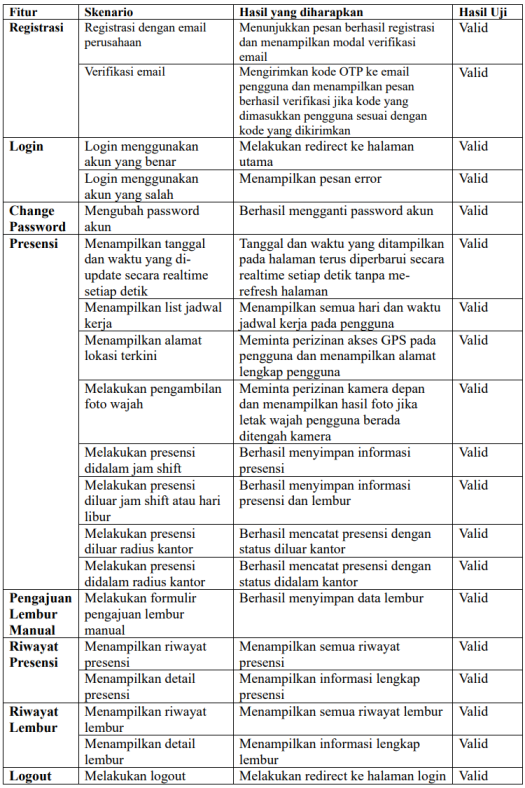
\includegraphics[width=0.8\textwidth]{Gambar/bab4/uat-staff-infrastructure-page-1.png}
\end{figure}
\FloatBarrier

\begin{figure}[!htbp]
	\centering
		
\includegraphics[width=0.8\textwidth]{Gambar/bab4/uat-staff-infrastructure-page-2.png}
\end{figure}
\FloatBarrier
\pagebreak

\nextappendix
\section*{Lampiran \theappendixletter: Hasil \textit{Blackbox Testing} Oleh \textit{Manager Human Resources}
\label{sec:blackbox-testing-aplikasi-presensi-online-oleh-manager-hrd}}
\addcontentsline{toc}{section}{Lampiran \theappendixletter: Hasil \textit{Blackbox Testing} Oleh \textit{Manager Human Resources}} 
\begin{figure}[!htbp]
	\centering
		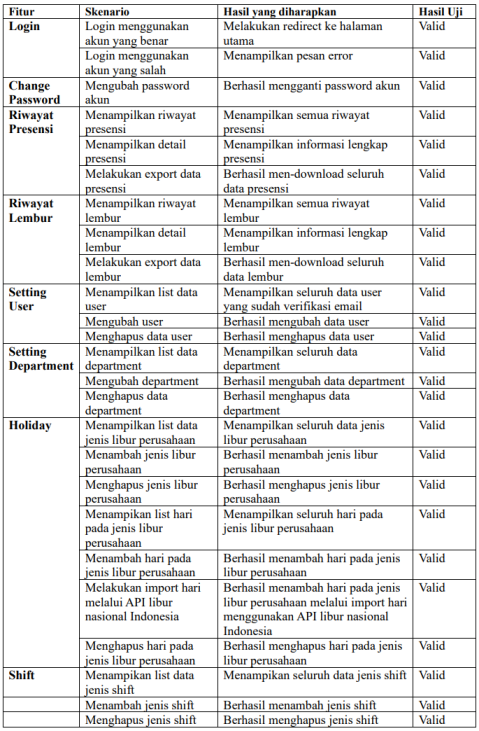
\includegraphics[width=0.8\textwidth]{Gambar/bab4/uat-manager-hrd-page-1.png}
\end{figure}
\FloatBarrier

\begin{figure}[!htbp]
	\centering
		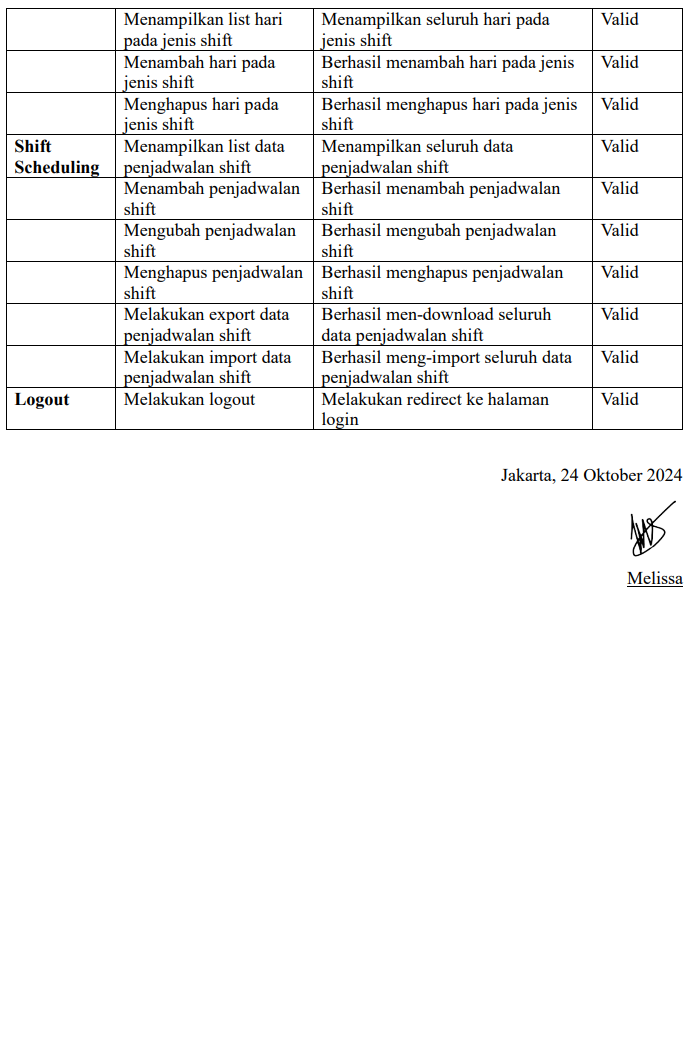
\includegraphics[width=0.8\textwidth]{Gambar/bab4/uat-manager-hrd-page-2.png}
\end{figure}
\FloatBarrier
\pagebreak

\nextappendix
\section*{Lampiran \theappendixletter: Hasil \textit{Blackbox Testing} Oleh \textit{Manager Infrastructure}
\label{sec:blackbox-testing-aplikasi-presensi-online-oleh-manager-infrastructure}}
\addcontentsline{toc}{section}{Lampiran \theappendixletter: Hasil \textit{Blackbox Testing} Oleh \textit{Manager Infrastructure}} 
\begin{figure}[!htbp]
	\centering
		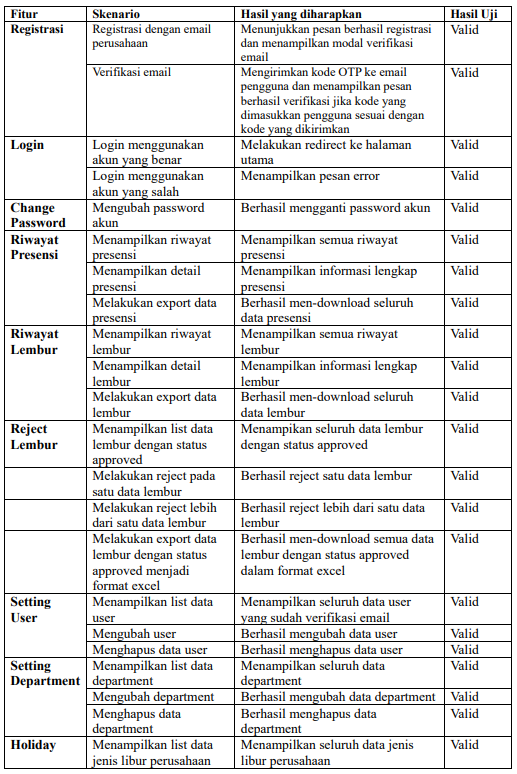
\includegraphics[width=0.8\textwidth]{Gambar/bab4/uat-manager-infrastructure-page-1.png}
\end{figure}
\FloatBarrier

\begin{figure}[!htbp]
	\centering
		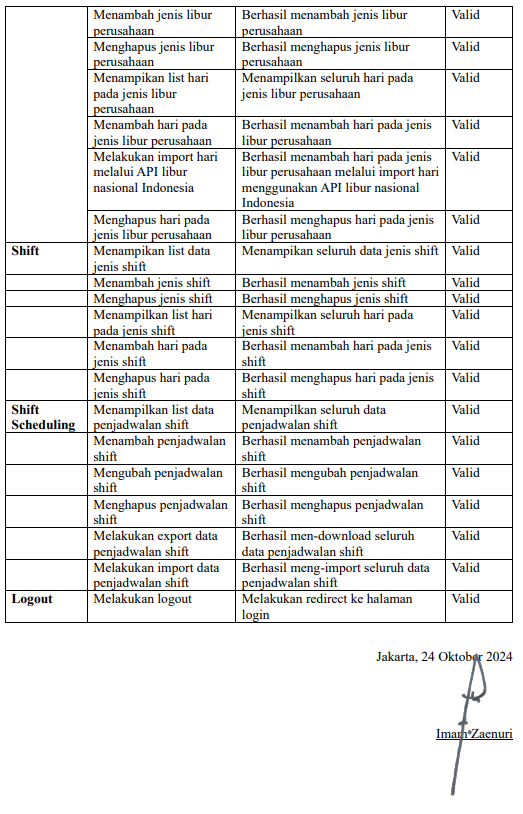
\includegraphics[width=0.8\textwidth]{Gambar/bab4/uat-manager-infrastructure-page-2.png}
\end{figure}
\FloatBarrier
\pagebreak

\nextappendix
\section*{Lampiran \theappendixletter: Dokumentasi \textit{Blackbox Testing} Bersama \textit{User}
\label{sec:dokumentasi-blackbox-testing}}
\addcontentsline{toc}{section}{Lampiran \theappendixletter: Dokumentasi \textit{Blackbox Testing} Bersama \textit{User}} 
\begin{figure}[!htbp]
	\centering
		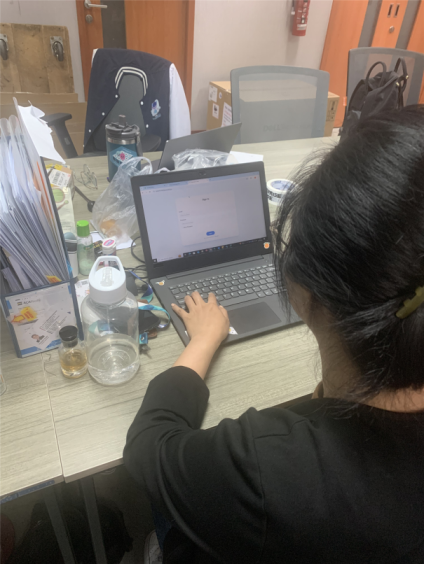
\includegraphics[width=0.8\textwidth]{Gambar/bab4/dokumentasi-staff-infra.png}
  \caption{Dokumentasi \textit{Blackbox Testing} Oleh \textit{Staff Infrastructure}}
	\label{fig:dokumentasi-blackbox-testing-oleh-staff-infrastructure}
\end{figure}
\FloatBarrier

\begin{figure}[!htbp]
	\centering
		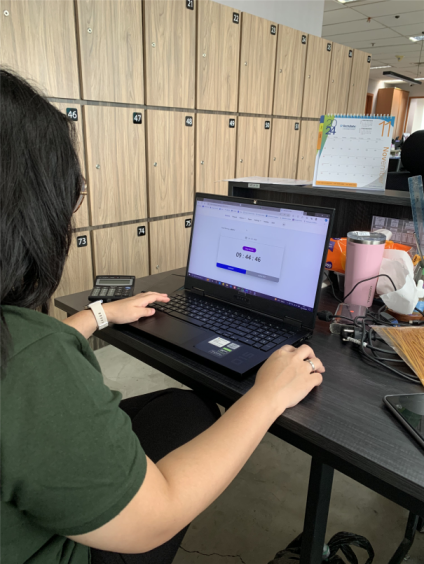
\includegraphics[width=0.8\textwidth]{Gambar/bab4/dokumentasi-manager-hrd.png}
    \caption{Dokumentasi \textit{Blackbox Testing} Oleh \textit{Manager Human Resources}}
	\label{fig:dokumentasi-blackbox-testing-oleh-manager-human-resources}
\end{figure}
\FloatBarrier

\begin{figure}[!htbp]
	\centering
		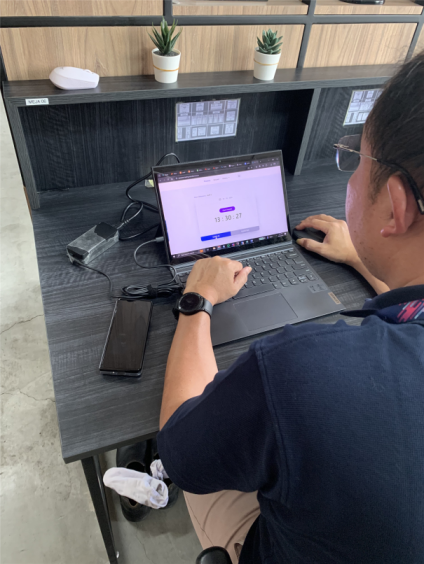
\includegraphics[width=0.8\textwidth]{Gambar/bab4/dokumentasi-manager-infra.png}
    \caption{Dokumentasi \textit{Blackbox Testing} Oleh \textit{Manager Infrastructure}}
	\label{fig:dokumentasi-blackbox-testing-oleh-manager-infrastructure}
\end{figure}
\FloatBarrier
\pagebreak

\nextappendix
\section*{Lampiran \theappendixletter: Hasil \textit{Blackbox Testing} Oleh Pengguna \textit{Non}-IT
\label{sec:blackbox-testing-aplikasi-presensi-online-oleh-pengguna-non-it}}
\addcontentsline{toc}{section}{Lampiran \theappendixletter: Hasil \textit{Blackbox Testing} Oleh Pengguna \textit{Non-}IT} 
\begin{figure}[!htbp]
	\centering
		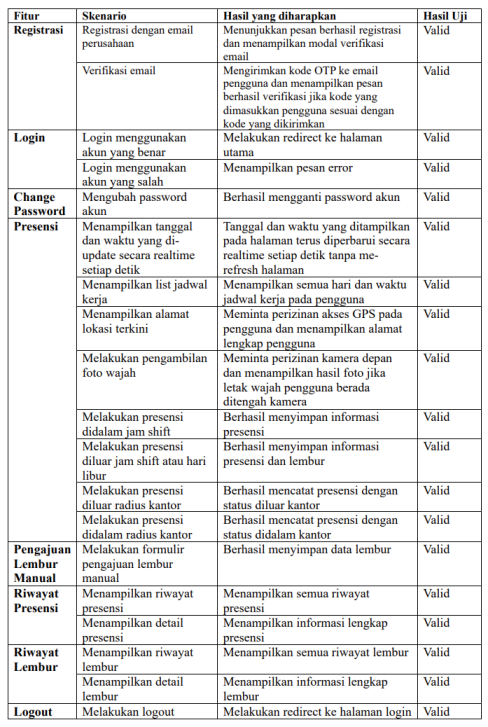
\includegraphics[width=0.8\textwidth]{Gambar/bab4/uat-non-it-1-page-1.png}
\end{figure}
\FloatBarrier

\begin{figure}[!htbp]
	\centering
		
\includegraphics[width=0.8\textwidth]{Gambar/bab4/uat-non-it-1-page-2.png}
\end{figure}
\FloatBarrier

\begin{figure}[!htbp]
	\centering
		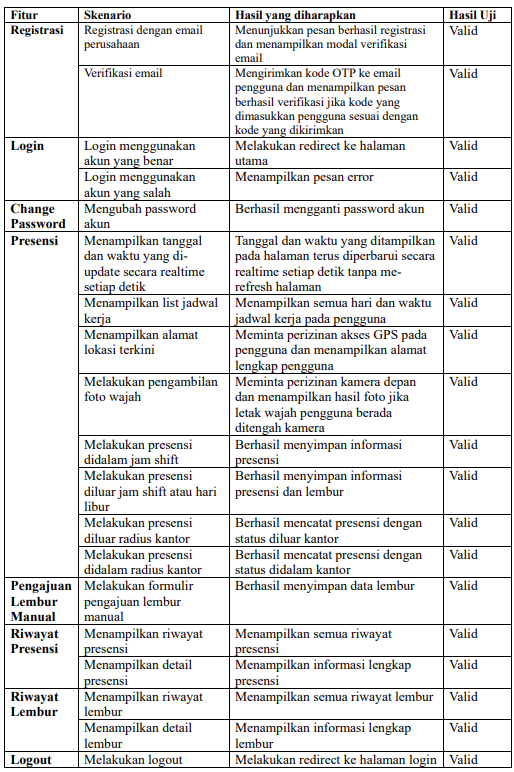
\includegraphics[width=0.8\textwidth]{Gambar/bab4/uat-non-it-2-page-1.png}
\end{figure}
\FloatBarrier

\begin{figure}[!htbp]
	\centering
		
\includegraphics[width=0.8\textwidth]{Gambar/bab4/uat-non-it-2-page-2.png}
\end{figure}
\FloatBarrier

\begin{figure}[!htbp]
	\centering
		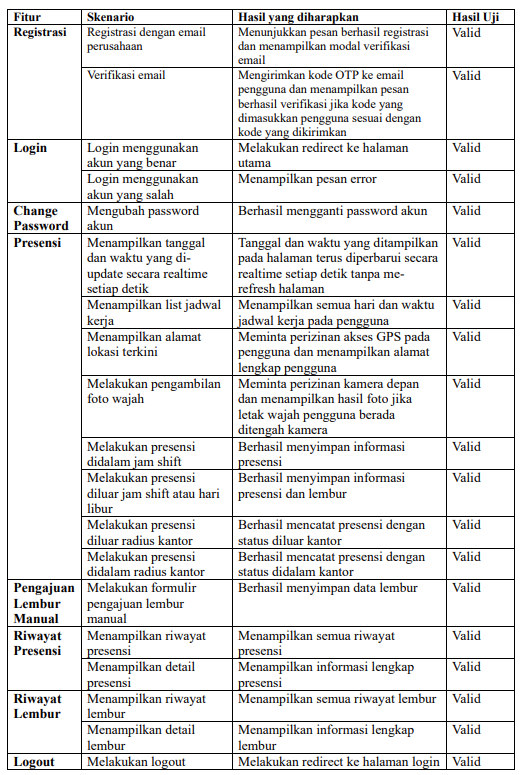
\includegraphics[width=0.8\textwidth]{Gambar/bab4/uat-non-it-3-page-1.png}
\end{figure}
\FloatBarrier

\begin{figure}[!htbp]
	\centering
		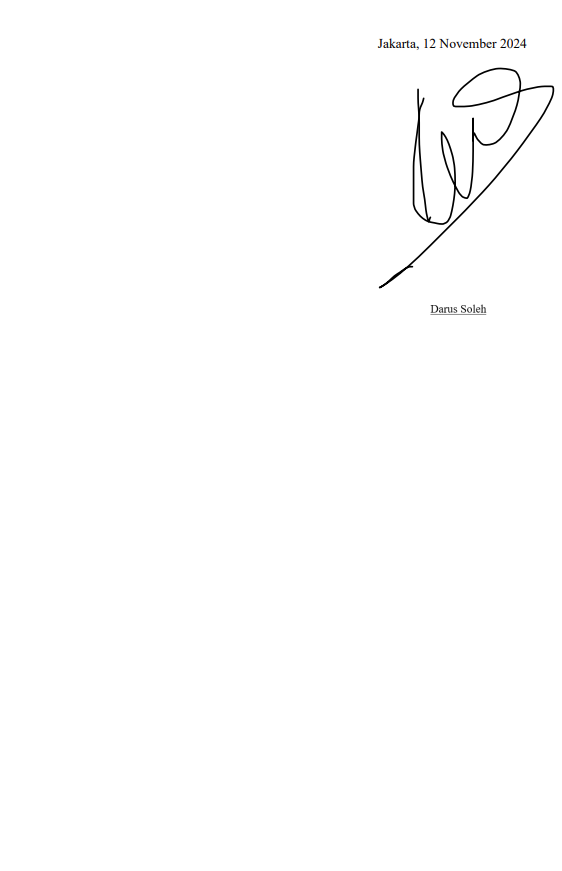
\includegraphics[width=0.8\textwidth]{Gambar/bab4/uat-non-it-3-page-2.png}
\end{figure}
\FloatBarrier

\begin{figure}[!htbp]
	\centering
		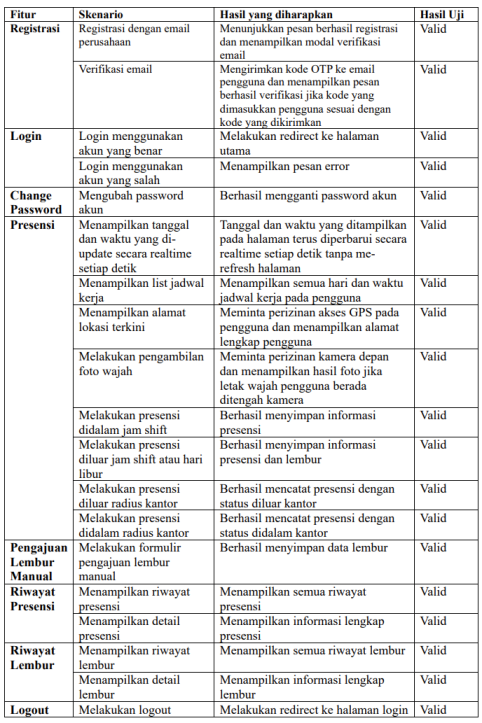
\includegraphics[width=0.8\textwidth]{Gambar/bab4/uat-non-it-4-page-1.png}
\end{figure}
\FloatBarrier

\begin{figure}[!htbp]
	\centering
		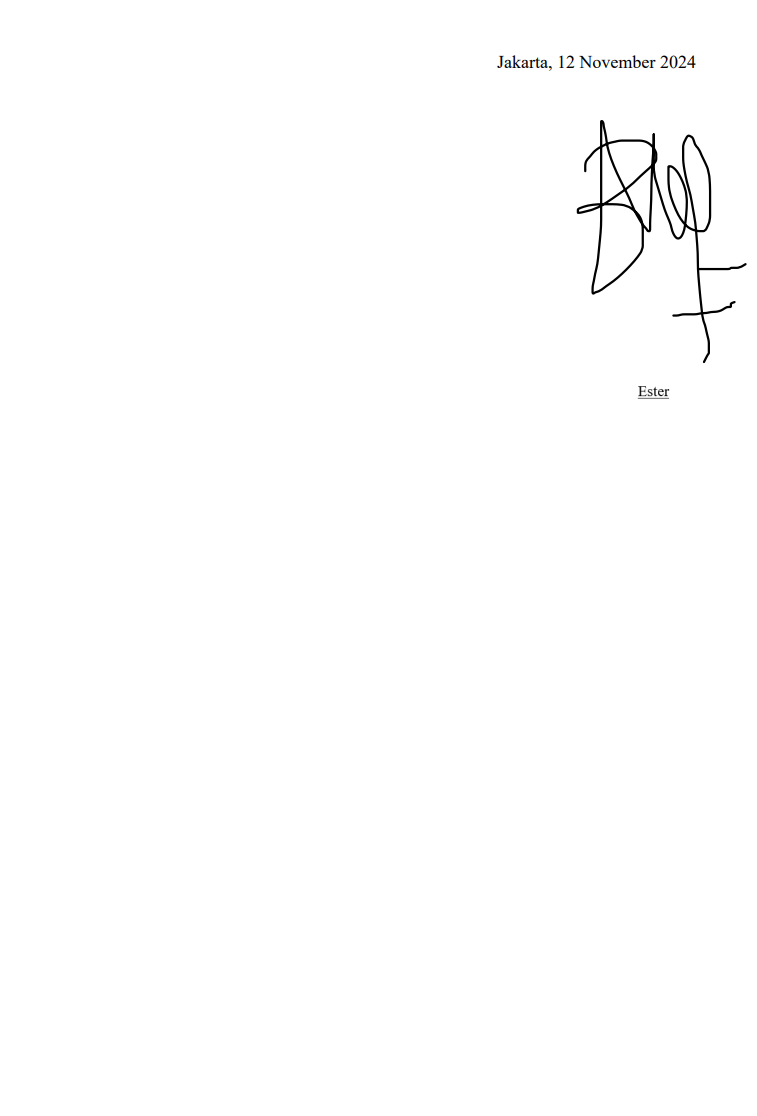
\includegraphics[width=0.8\textwidth]{Gambar/bab4/uat-non-it-4-page-2.png}
\end{figure}
\FloatBarrier

\begin{figure}[!htbp]
	\centering
		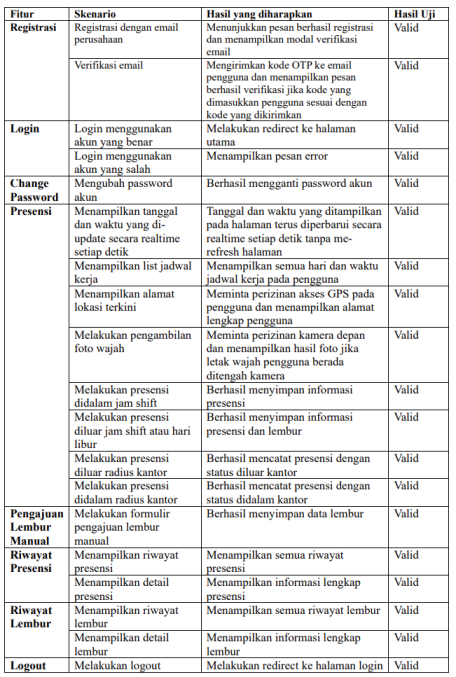
\includegraphics[width=0.8\textwidth]{Gambar/bab4/uat-non-it-5-page-1.png}
\end{figure}
\FloatBarrier

\begin{figure}[!htbp]
	\centering
		
\includegraphics[width=0.8\textwidth]{Gambar/bab4/uat-non-it-5-page-2.png}
\end{figure}
\FloatBarrier

\begin{figure}[!htbp]
	\centering
		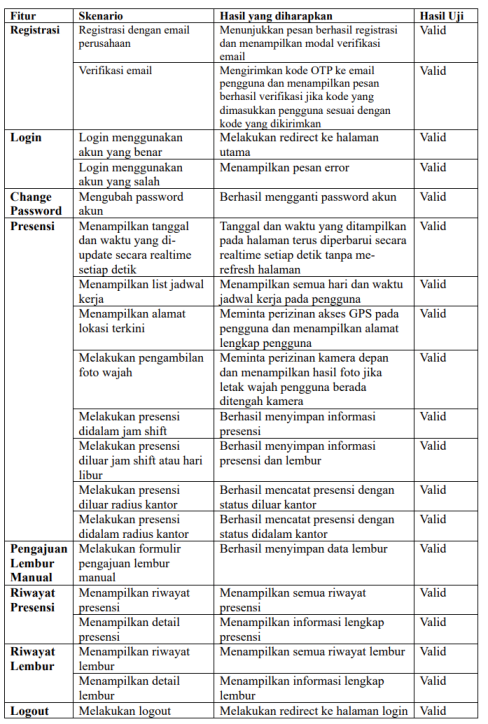
\includegraphics[width=0.8\textwidth]{Gambar/bab4/uat-non-it-6-page-1.png}
\end{figure}
\FloatBarrier

\begin{figure}[!htbp]
	\centering
		
\includegraphics[width=0.8\textwidth]{Gambar/bab4/uat-non-it-6-page-2.png}
\end{figure}
\FloatBarrier

\begin{figure}[!htbp]
	\centering
		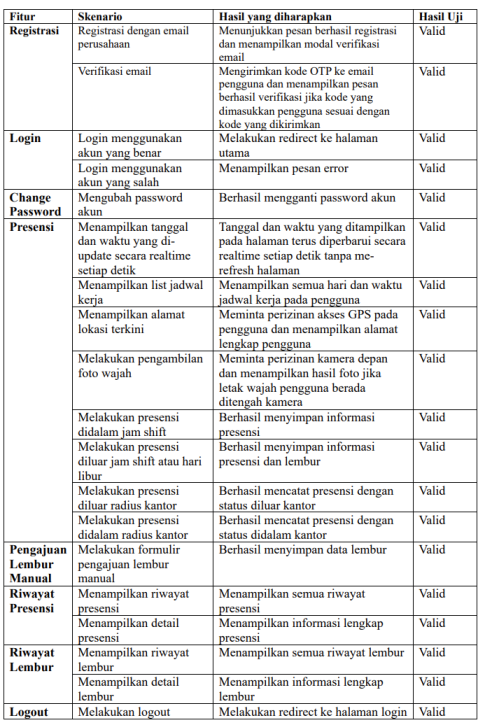
\includegraphics[width=0.8\textwidth]{Gambar/bab4/uat-non-it-7-page-1.png}
\end{figure}
\FloatBarrier

\begin{figure}[!htbp]
	\centering
		
\includegraphics[width=0.8\textwidth]{Gambar/bab4/uat-non-it-7-page-2.png}
\end{figure}
\FloatBarrier

\begin{figure}[!htbp]
	\centering
		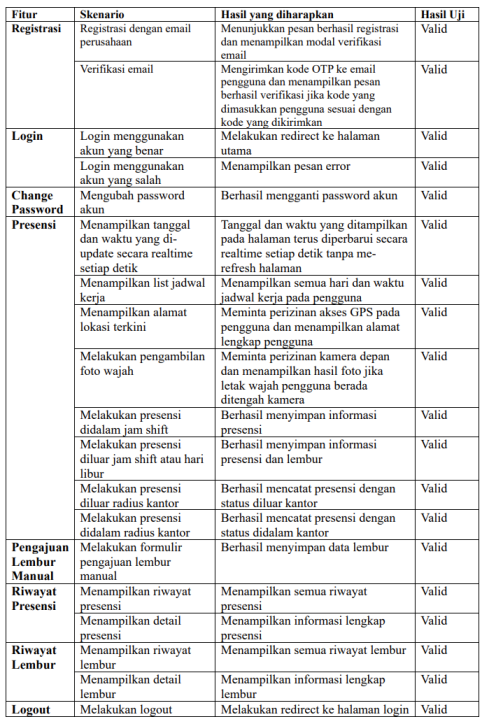
\includegraphics[width=0.8\textwidth]{Gambar/bab4/uat-non-it-8-page-1.png}
\end{figure}
\FloatBarrier

\begin{figure}[!htbp]
	\centering
		
\includegraphics[width=0.8\textwidth]{Gambar/bab4/uat-non-it-8-page-2.png}
\end{figure}
\FloatBarrier

\begin{figure}[!htbp]
	\centering
		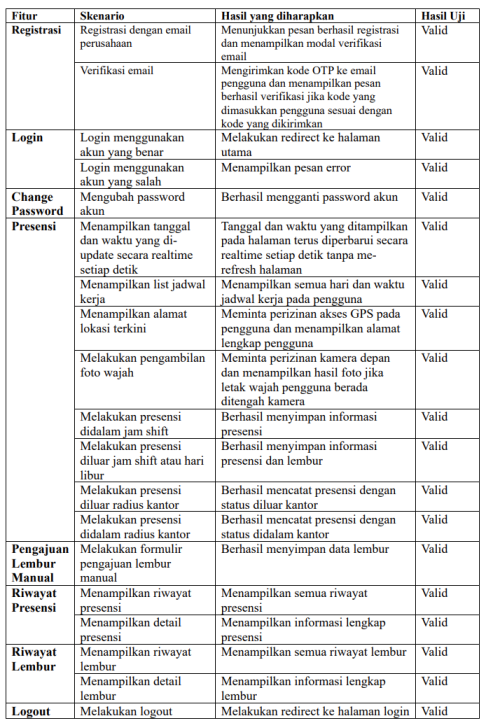
\includegraphics[width=0.8\textwidth]{Gambar/bab4/uat-non-it-9-page-1.png}
\end{figure}
\FloatBarrier

\begin{figure}[!htbp]
	\centering
		
\includegraphics[width=0.8\textwidth]{Gambar/bab4/uat-non-it-9-page-2.png}
\end{figure}
\FloatBarrier

\begin{figure}[!htbp]
	\centering
		\includegraphics[width=0.8\textwidth]{Gambar/bab4/uat-non-it-10-page-1.png}
\end{figure}
\FloatBarrier

\begin{figure}[!htbp]
	\centering
		\includegraphics[width=0.8\textwidth]{Gambar/bab4/uat-non-it-10-page-2.png}
\end{figure}
\FloatBarrier
\pagebreak

\nextappendix
\section*{Lampiran \theappendixletter: Dokumentasi \textit{Blackbox Testing} dan SUS Bersama \textit{Staff Non-}IT
\label{sec:dokumentasi-blackbox-testing-dan-sus-bersama-staff-non-it}}
\addcontentsline{toc}{section}{Lampiran \theappendixletter: Dokumentasi \textit{Blackbox Testing} dan SUS Bersama \textit{Staff Non-}IT}
\begin{figure}[!htbp]
	\centering
	\includegraphics[width=0.8\textwidth]{Gambar/bab4/uat-bilal.png}
  \caption{Dokumentasi \textit{Blacbox Testing} dan SUS Bersama Bapak Bilal}
	\label{fig:dokumentasi-uat-sus-bersama-bapak-bilal}
\end{figure}
\FloatBarrier

\begin{figure}[!htbp]
	\centering
	\includegraphics[width=0.8\textwidth]{Gambar/bab4/uat-chairul.png}
  \caption{Dokumentasi \textit{Blacbox Testing} dan SUS Bersama Bapak Chairul}
	\label{fig:dokumentasi-uat-sus-bersama-bapak-chairul}
\end{figure}
\FloatBarrier

\begin{figure}[!htbp]
	\centering
	\includegraphics[width=0.8\textwidth]{Gambar/bab4/uat-darus.png}
  \caption{Dokumentasi \textit{Blacbox Testing} dan SUS Bersama Bapak Darus}
	\label{fig:dokumentasi-uat-sus-bersama-bapak-darus}
\end{figure}
\FloatBarrier

\begin{figure}[!htbp]
	\centering
	\includegraphics[width=0.8\textwidth]{Gambar/bab4/uat-ester.png}
  \caption{Dokumentasi \textit{Blacbox Testing} dan SUS Bersama Ibu Ester}
	\label{fig:dokumentasi-uat-sus-bersama-ibu-ester}
\end{figure}
\FloatBarrier

\begin{figure}[!htbp]
	\centering
	\includegraphics[width=0.8\textwidth]{Gambar/bab4/uat-hany.png}
  \caption{Dokumentasi \textit{Blacbox Testing} dan SUS Bersama Ibu Hany}
	\label{fig:dokumentasi-uat-sus-bersama-ibu-hany}
\end{figure}
\FloatBarrier

\begin{figure}[!htbp]
	\centering
	\includegraphics[width=0.8\textwidth]{Gambar/bab4/uat-heri.png}
  \caption{Dokumentasi \textit{Blacbox Testing} dan SUS Bersama Bapak Heri}
	\label{fig:dokumentasi-uat-sus-bersama-bapak-heri}
\end{figure}
\FloatBarrier

\begin{figure}[!htbp]
	\centering
	\includegraphics[width=0.8\textwidth]{Gambar/bab4/uat-nada.png}
  \caption{Dokumentasi \textit{Blacbox Testing} dan SUS Bersama Ibu Nada}
	\label{fig:dokumentasi-uat-sus-bersama-ibu-nada}
\end{figure}
\FloatBarrier

\begin{figure}[!htbp]
	\centering
	\includegraphics[width=0.8\textwidth]{Gambar/bab4/uat-rudi.png}
  \caption{Dokumentasi \textit{Blacbox Testing} dan SUS Bersama Bapak Rudi}
	\label{fig:dokumentasi-uat-sus-bersama-bapak-rudi}
\end{figure}
\FloatBarrier

\begin{figure}[!htbp]
	\centering
	\includegraphics[width=0.8\textwidth]{Gambar/bab4/uat-salwa.png}
  \caption{Dokumentasi \textit{Blacbox Testing} dan SUS Bersama Ibu Salwa}
	\label{fig:dokumentasi-uat-sus-bersama-ibu-salwa}
\end{figure}
\FloatBarrier

\begin{figure}[!htbp]
	\centering
	\includegraphics[width=0.8\textwidth]{Gambar/bab4/uat-yuli.png}
  \caption{Dokumentasi \textit{Blacbox Testing} dan SUS Bersama Ibu Yuliana}
	\label{fig:dokumentasi-uat-sus-bersama-ibu-yuliana}
\end{figure}
\FloatBarrier

\pagebreak




